\documentclass[10pt,twocolumn,letterpaper,UTF8]{article}
\hyphenpenalty=2000
\textwidth=6.5in
\textheight=9.0in
\evensidemargin=0.0in
\oddsidemargin=0.0in
\topmargin=-0.5in
\clubpenalty=4000
\widowpenalty=4000
\displaywidowpenalty=500

\newlength\minalignvsep

\usepackage{cvpr}
\usepackage{times}
\usepackage{epsfig}
\usepackage{graphicx}
\usepackage{amsmath,amssymb,amsthm}
\usepackage{pbox}
\usepackage{epstopdf}
\usepackage{subfigure}
\usepackage{xspace}
\usepackage{comment}
\usepackage{lipsum}
%\usepackage{jeffe}
\usepackage{enumitem}

% 中文支持
\usepackage{ctex}
\usepackage[T1]{fontenc}
\usepackage{mathpazo}
\usepackage{fontspec}
\setmainfont[Scale = 1]{TeX Gyre Pagella}
\setCJKmainfont[ItalicFont=Noto Serif CJK SC Bold, BoldFont=Noto Serif CJK SC Black, Scale = 1]{Noto Serif CJK SC}

\newcommand{\cmt}[2]{[#1: #2]}
\newcommand{\todo}[1]{\cmt{{\bf TODO}}{{\bf \color{red} #1}}}
\newcommand{\hao}[1]{\cmt{{\bf Hao}}{{\bf \color{red} #1}}}
\newcommand{\rqi}[1]{\cmt{{\bf Charles}}{{\bf \color{blue} #1}}}
\newcommand{\km}[1]{\cmt{{\bf Kaichun}}{{\bf \color{green} #1}}}
\newcommand{\leo}[1]{\cmt{{\bf Leo}}{{\bf \color{cyan} #1}}}

\newcommand{\shape}{S}
\newcommand{\image}{I}
\newcommand{\network}{\mathbb{G}}
\newcommand{\prob}{\mathcal{P}}

\newcommand{\para}[1]{\noindent{\bf #1}}

\newcommand{\softpara}{\paragraph}
\newcommand{\mypara}{\vspace*{-15pt}\paragraph}

\newcommand{\bmemo}[1]{\noindent{\color{blue}{\sf [[#1]]}}}

\newcommand{\denselist}{\itemsep 0pt\parsep=0pt\partopsep 0pt\vspace{-2pt}}
\newcommand{\bitem}{\begin{itemize}\denselist}
\newcommand{\eitem}{\end{itemize}}
\newcommand{\benum}{\begin{enumerate}\denselist}
\newcommand{\eenum}{\end{enumerate}}
\newcommand{\bdescr}{\begin{description}\denselist}
\newcommand{\edescr}{\end{description}}

\newcommand{\Remark}[1]     {{\sf [#1]}}

\setlength{\abovedisplayskip}{0pt}
\setlength{\belowdisplayskip}{0pt}

\newtheorem{theorem}{Theorem}

\newcommand{\myvec}[1]{\mathbf #1}
\newcommand\blfootnote[1]{%
  \begingroup
  \renewcommand\thefootnote{}\footnote{#1}%
  \addtocounter{footnote}{-1}%
  \endgroup
}
\newtheorem{innercustomthm}{Theorem}
\newenvironment{customthm}[1]
  {\renewcommand\theinnercustomthm{#1}\innercustomthm}
  {\endinnercustomthm}
  
% Include other packages here, before hyperref.

% If you comment hyperref and then uncomment it, you should delete
% egpaper.aux before re-running latex.  (Or just hit 'q' on the first latex
% run, let it finish, and you should be clear).
\usepackage[pagebackref=true,breaklinks=true,letterpaper=true,colorlinks,bookmarks=false]{hyperref}

\cvprfinalcopy % *** Uncomment this line for the final submission

\def\cvprPaperID{201} % *** Enter the CVPR Paper ID here
\def\httilde{\mbox{\tt\raisebox{-.5ex}{\symbol{126}}}}

% Pages are numbered in submission mode, and unnumbered in camera-ready
\ifcvprfinal\pagestyle{empty}\fi
\begin{document}

%%%%%%%%% TITLE
\title{PointNet: 针对三维分类点云分类与分割的深度学习模型
% PointNet: Deep Learning on Point Sets for 3D Classification and Segmentation
}

% \author{First Author\\
% Institution1\\
% Institution1 address\\
% {\tt\small firstauthor@i1.org}
% % For a paper whose authors are all at the same institution,
% % omit the following lines up until the closing ``}''.
% % Additional authors and addresses can be added with ``\and'',
% % just like the second author.
% % To save space, use either the email address or home page, not both
% \and
% Second Author\\
% Institution2\\
% First line of institution2 address\\
% {\tt\small secondauthor@i2.org}
% }

\author{Charles R. Qi*\qquad Hao Su* \qquad Kaichun Mo \qquad Leonidas J. Guibas\\Stanford University\\翻译: 浙江大学软件学院 2021 年夏令营 CAD 第三小组}

\maketitle
%\thispagestyle{empty}

%%%%%%%%% ABSTRACT
\begin{abstract}
{\normalfont
  % - input is very special, other people do qualization, have problem
% - we directly consume point set by unified architecture, for object classication, part seg, and scene seg
% - our network is simple. it respects the permutuation inv by max pooling. 
% - the method is very effective, supported by theoretical analysis and experimental evidences.

点云是一种重要的几何数据结构。由于其无序性,大多数研究者将这些数据转换为有序的三维体素网格或图像集合。然而,这会导致不必要的数据冗余并引起一些问题。在本文中,我们设计了一种直接处理点云的新型神经网络,这种网络很好的考虑了输入中的点的置换不变性。我们构建了名叫PointNet的神经网络,它为物体分类、零件分割和场景语义分析等应用程序提供了统一的结构。PointNet结构虽然简单,但却十分高效且有效。从经验上,它表现出了与现有技术水平相当甚至更好的性能。从理论上,我们为解释这种网络学习到了什么和为什么这种网络能够对输入数据的扰动和损坏保持高度健壮性进行了分析。



   
% \begin{figure}[h!]
%     \centering
%     
\includegraphics[width=\linewidth,height=5cm]{fig/placeholder}
% \end{figure}

}
\end{abstract}

%%%%%%%%% BODY TEXT
\section{引入}
\blfootnote{* 表示同等贡献。}
\label{sec:intro}


本文探索了能够处理3D几何数据比如点云和网格的深度学习模型。为了实现权重分享和其他核函数优化,典型的卷积结构要求输入数据的格式高度规则,比如图形网格和3D体素。由于点云或网格并不是有序格式,大多数研究人员通常会将这些数据转换为常规的3D体素或图像集合(例如视图),然后再将它们输入到深层网络中。然而,这种数据表示转换会使结果数据变不必要的大量增加,同时也会引入能模糊数据自然不变性的量化伪影。

因此我们重点介绍一种不同于以往只使用简单点云的3D几何神经网络,并将其命名为PointNets。点云是简单且统一的结构,能够避免网格的组合不规则性和复杂性,因此更容易学习。然而,PointNet依旧受限于点云只是点的一个集合这样一个事实,因此其内部元素的排列是不变的,需要在网络计算中做一些对称性处理。而更进一步的刚性运动的不变性也需要考虑。

我们构建的PointNet是一个统一的架构,这体现在将点云作为输入,输出整体输入或相对于输入的部分点块的类标签。该模型的基础构架非常的简单,因为在初始阶段,每个点的处理方法完全相同且独立。在基础设置中,每个点仅用它的三个坐标(x,y,z)来表示。额外维度可以通过计算法线和其他局部或者全局特征来添加得到。

我们这个方法的关键在于使用对称的max pooling函数。网络有效地学习一组优化函数/准则,从点云中选择感兴趣的点或者含有信息的点,并编码选择的原因。网络最终的全连接层把这些学习到的最优值聚合到如上所述的整个形状的全局描述符(形状分类)上或者用于预测每个点标签(形状分割)。

我们的输入格式很容易应用刚性或者仿射变换,因为每个点都是独立变换的。因此我们可以在应用PointNet处理点云之前添加一个与数据无关的空间转换网络来规范化点云数据,以此来进一步提高结果的表现。

我们提供了方法的理论分析和实验评估,展示了我们的网路可以近似任何连续的集合函数。更有趣的是,事实证明我们的网络通过学习一组稀疏的关键点来概括一个输入点云,这些关键点根据可视化结果在视觉上大致对应对象的骨架。理论分析解释了为什么我们的PointNet对于输入点云的微小扰动,以及由极端点插入或删除点带来的数据损坏有着良好的健壮性。

我们对大量参照数据集(包括形状分类、零件分割、场景分割)进行实验,比较了PointNet和目前基于多视角与体积表示的最先进的方法。在统一的构架下,PointNet不仅在速度上更快,同时也表现出了和现有技术相当甚至更好的性能。
我们工作的主要贡献如下:
\begin{itemize}
    \item 我们设计了一个适用于处理3D无序点集的新型深度网络模型
    \item 我们展示了如何训练这样的网络模型来处理3D形状分类、零件分割和场景语义分析等任务
    \item 我们从实验和理论的角度分析了方法的稳定性和效率
    \item 我们演示了网络中所选择神经元计算出的3D特征,并对其性能进行了直观的解释
    
\end{itemize}
使用神经网络处理无序集合的问题是一个非常普遍和根本的问题,我们希望我们的想法也可以应用到其他领域。


\begin{figure}
    \centering
    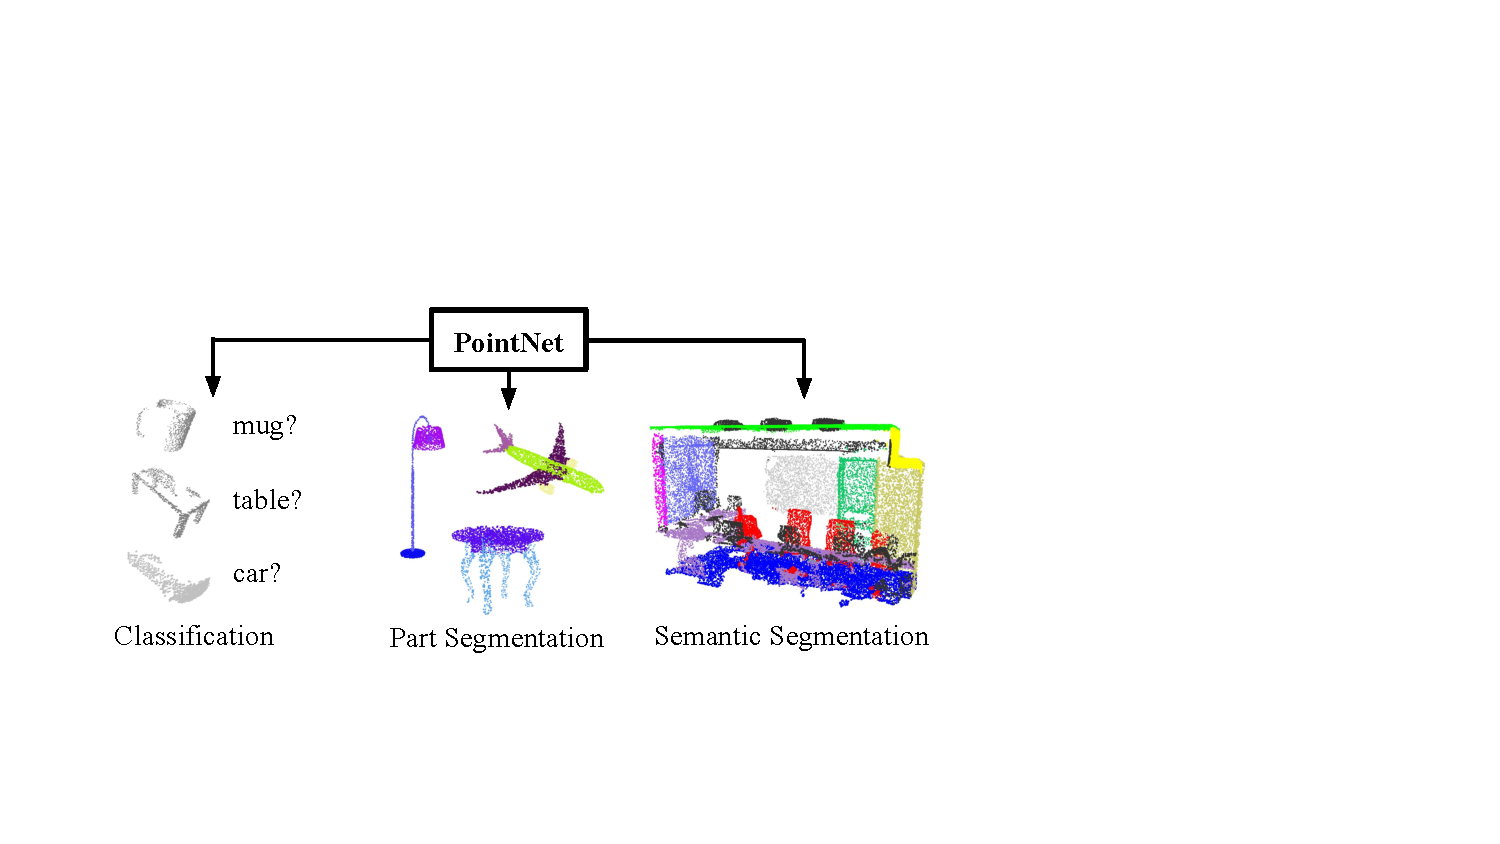
\includegraphics[width=\linewidth]{fig/teaser.pdf}
    \caption{\textbf{PointNet 的应用} 
    我们提出了一个新的神经网络结构,其输入为一个原始的点云(点的集合),没有经过体素化或预渲染。该网络具有一个统一的架构,能够学习全局和局部的点特征,从而为各种三维识别任务提供了一个简单、高速而有效的方法。 
    %We propose a novel deep net architecture that consumes raw point cloud (set of points) without voxelization or rendering. It is a unified architecture that learns both global and local point features, providing a simple, efficient and effective approach for a number of 3D recognition tasks.% 
    }
    \label{fig:teaser}
\end{figure}


\begin{figure*}[th!]
    \centering
    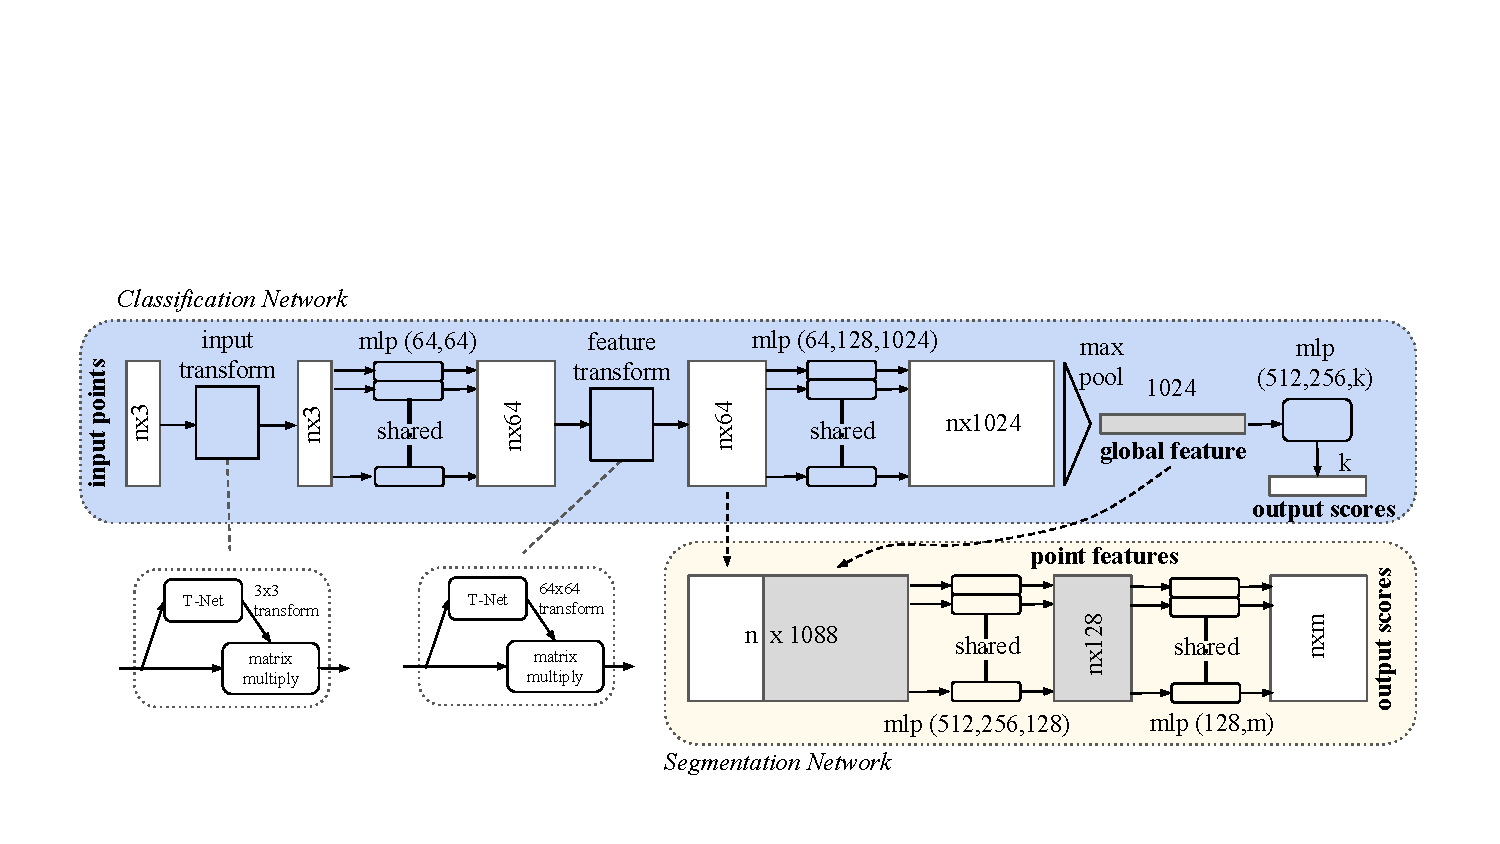
\includegraphics[width=0.9\linewidth]{fig/pointnet_fixed.pdf}
    \caption{\textbf{PointNet 架构}      分类网络将$n$个点作为输入,作用输入和特征变换,然后通过max pooling聚合点的特征,输出的是$k$种分类的分类分数。分割网络是分类网络的拓展,它连接局部和全局特征以及每个点输出的分数。``mlp''代表多层感知机,括号中的数字是层的大小。Batchnorm用于所有应用了ReLU的层。Dropout用于分类网络中的最后一个多层感知机。}
    \label{fig:pointnet_arch}
\end{figure*}

\section{相关工作}
\label{sec:related}
\begin{comment}
\todo{\\
  \paragraph{3d point cloud processing:}
  \begin{itemize}
    \item classification
    \item segmentation
    % \item correspondence
  \end{itemize} 
  traditionally, each 3d data processing task depends on some specific pipeline. our framework unifies them together.
  
  \paragraph{point cloud features:}
  \begin{itemize}
    \item global features
    \item local features
  \end{itemize}
  most works use hand-crafted features. 

  \paragraph{deep learning on 3d data:}
  \begin{itemize}
    \item multi-view CNN
    \item volumetric CNN
    \item spectral CNN on meshes 
    \item non end-to-end approach
  \end{itemize}
  in previous work of deep learning on point clouds, a point cloud is first converted to one of the above forms. however, there lacks work that directly operates on a raw point set.

  \paragraph{deep learning on unordered sets}
  \begin{itemize}
    \item discuss ``OrderMatters'', by Vinyals et al.
    \item say that this is a rather fundamental problem, related to many other tasks
  \end{itemize} 
}
\end{comment}

\paragraph{点云特征}
点云大部分的现有特征都是针对特定任务手工制作的。点特征通常编码某些统计特性,并且被设计成对于某些变换是不变的,这些变换通常被划分为内在的
\cite{aubry2011wave, sun2009concise, bronstein2010scale} 或外在的 ~\cite{rusu2008aligning, rusu2009fast, ling2007shape, johnson1999using, chen2003visual}。  它们还可以归类为局部特征和全局特征。对于特定任务,找到最优的特征组合并非易事。

%While one can extract all kinds of features and let a machine learning model decide which ones to use, the success of CNNs~\cite{lecun2015deep} for 2D images convinces us that an end-to-end feature learning paradigm is more promising. In this work we present a unified point feature learning network that can easily adapts to different tasks.

% \paragraph{Point Cloud Features}
% Most existing features for point cloud are handcrafted towards specific tasks. According to the spatial scopes, they can be categorized as local features and global features. Point features often encode certain statistical properties of points and are designed to be invariant to certain transformations, which are typically classified as being intrinsic [WKS, HKS] or extrinsic [PFH, FPFH, D2, spin image, LFD].

% Often one feature that works on task A may not perform well on task B. In addition, different features often make different assumptions of where the point cloud comes from. For example, HKS and WKS features work very well on organic objects such as human bodies, but they are not suitable for describing CAD models with combinatorial structures. For a specific task, it is not trivial to find the optimal feature combination for the task. 

% While one can extract all kinds of features and let a machine learning model to decide which ones to use, the success of CNNs [CITE] for 2D images convinces us that an end-to-end feature learning paradigm is more promising. In this work we present a unified point feature learning network that can easily adapts to different tasks, such as classification, segmentation, retrieval and correspondence. Our network directly works on point sets, due to its flexibility and broad usage in real applications.


\paragraph{3D数据的深度学习}
% \todo{we need to argue why point cloud (most close to raw sensor data), instead of meshes (not canonical), volume (sparsity), projected images (not in 3D, non-trivial to choose viewpoints) somewhere in the paper.}

3D数据具有多种流行的表示形式,从而有各种学习方法。
\emph{Volumetric CNNs:}~\cite{wu20153d, maturana2015voxnet, qi2016volumetric} 这是在体素形状上应用3D卷积神经网络的先驱。然而,由于数据的稀疏性和3D卷积的计算成本,体积表示受到其分辨率的限制。FPNN~\cite{li2016fpnn} 和 Vote3D~\cite{wang2015voting} 提出了处理稀疏性问题的特殊方法;然而,他们的操作仍然是在稀疏的体积上,处理非常大的点云对他们来说是一种挑战。
\emph{Multiview CNNs:}~\cite{su15mvcnn, qi2016volumetric} 试图将3D点云或形状渲染成2D图像,然后应用2D卷积神经网络对它们进行分类。通过精心设计的图像CNN,这一系列方法在形状分类和检索任务方面取得了突出的性能表现。~\cite{savvashrec}. 然而,将它们扩展到场景理解或其他3D任务例如点分类、形状完成上时表现很普通。
\emph{Spectral CNNs:} 最近的一些工作~\cite{bruna2013spectral, masci2015geodesic}在网格上使用了光谱CNN。但是这些方法目前受限于流形网格(例如有机物体),而且如何将它们扩展到非等距形状(例如家具)上并不明显。
\emph{Feature-based DNNs:}~\cite{fang20153d,guo20153d} 首先通过提取传统的形状特征将3D数据转换成向量,然后使用全连接网络对形状进行分类。我们认为它们受限于所提取特征的表示能力。

% In our work, we do deep learning directly on the raw 3D representation -- point clouds, without the pre-processing stage of converting them to volumes, images, graphs, or feature vectors. Therefore, our method has the potential to greatly simply the pipeline in practical usage.

% We argue that point cloud is a good representation in many aspects: 1) it's raw -- point clouds are the data acquired directly from depth sensors or laser scans, not like volumes or images that suffer from information loss. 2) it's in 3D, not like projected images that lack 3D geometry, which may require additional cross-view consistency mechanisms. 3) it's compact, not like volumetric grids that stores a 2D manifold surface in full 3D space. We design special networks to consume 3D point clouds and show that our network can be easily adapted for various 3D tasks with very good performance.


% Volumetric CNNs: [3DShapeNets, voxnet, our cvpr work] are the pioneers applying 3D convolutional neural networks on voxelized shapes. However, since sensors can only reach the surfaces of objects, most 3D data are just 2D manifold/surface living in a 3D space, thus volumetric grids are often sparse. Besides, the storage and computation cost both grow cubically with the input resolution. To address this challenge, [FPNN and vote3D] propose special methods to deal with the sparsity of volumetric representation; however, their operations are still performed on a very sparse volume and it is still challenging for them to process very large point clouds.

% Multiview CNNs: [MVCNN, our cvpr work, and some other image based methods] have tried to render 3D point cloud or shapes into 2D images and then apply 2D convolutional neural networks (using existing architectures such as AlexNet and VGG fine-tuned from ImageNet) to classify the shapes. With the well engineered image CNNs, this line of methods have achieved dominating performance on shape classification and retrieval tasks [cite SHREC]. However, it's nontrivial to extend them to scene understanding (not clear which camera positions to take), or other 3D tasks such as point classification and shape completion. Besides, when projecting 3D into images, we always have to convert predictions and data back and forth between 2D and 3D.

% Spectral CNNs: There has also been latest work that use spectral CNNs on meshes. However, these methods are currently constrained on manifold meshes such as organic objects and it's not obvious how to extend them to non-isometric shapes with sophisticated topological and geometric variations, such as furniture. Besides, acquiring meshes or point graphs require significant efforts in post processing from raw sensor data.

% Feature-based DNNs: [deep3dshape and Beihang's paper] firstly convert the 3D data into a vector, by extracting traditional shape features (HKS and WKS) and then use a fully connected neural network to classify the shape. We think they are constrained by the representation power of the features extracted.

% In our work, we do deep learning directly on the raw 3D representation -- point clouds, without the pre-processing stage of converting them to volumes, images, graphs, or feature vectors. Therefore, our method has the potential to greatly simply the pipeline in practical usage. We argue that point cloud is a good representation in many aspects: 1) it's raw -- point clouds are the data acquired directly from depth sensors or laser scans, not like volumes or images that suffer from information loss. 2) it's in 3D, not like projected images that lack 3D geometry, which may require additional cross-view consistency mechanisms. 3) it's compact, not like volumetric grids that stores a 2D manifold surface in full 3D space. We design special networks to consume 3D point clouds and show that our network can be easily adapted for various 3D tasks with very good performance.


\paragraph{无序集的深度学习}

从数据结构的角度来说,点云是无序的向量集合。当大部分深度学习工作集中在规则输入表示,如序列(语音和语言处理)、图像和体积(视频或3D数据)上时,很少有在点集上做深度学习工作的。

Oriol Vinyals等人最近的一项工作~\cite{vinyals2015order}研究了这个问题。他们使用具有注意机制的读取-处理-写入网络来处理无序输入集,同时展示他们的网络具有对数字进行排序的能力。然而,由于他们的工作重点是泛型集合和NLP应用,因此缺少了几何体在集合中的作用。

% Our work exploits the geometry properties in 3D point sets, provides theoretical analysis to what has been learned, gives rich visualizations to help understand the model. Our work also targets towards real applications of object classification and segmentation.

\section{问题陈述}
\label{sec:problem}
\begin{comment}
\todo{
  \begin{enumerate}
    \item we are interested in deep learning methods for object classification and segmentation on 3d point sets.
    \item we solve the two problems in a unified framework. in this framework, we use neural network to learn a function $f$ that takes a subset of points in $\R^3$ as input, and predicts the object recognition or per-point segmentation.  
  \end{enumerate}
}
\end{comment}

我们设计了一个能够将无序的点集作为输入的深度学习网络框架。一个点云可以由若干个三维点的集合表示 $\{P_i| \ i=1,...,n\}$,其中每个点 $P_i$ 都是其空间坐标 $(x,y,z)$ 和其他额外的特征频道(例如颜色、范数等)。出于简洁性和清晰性,除非特别指出,我们只使用三维空间坐标,即 $(x,y,z)$ 作为输入点的频道。

% We design a deep learning framework that directly consumes unordered point sets as inputs. %, while most recent state-of-the-art methods convert them to volumetric grids \cite{wu20153d,wang2015voting,qi2016volumetric} or projecting them to images \cite{su15mvcnn,qi2016volumetric}. % Furthermore, our proposed network is a unified framework for a various of applications including object classification, object-level part segmentation and scene semantic parsing. A point cloud is represented as a set of 3D points $\{P_i| \ i=1,...,n\}$, where each point $P_i$ is a vector of its $(x,y,z)$ coordinate plus extra feature channels such as color, normal etc. For simplicity and clarity, unless otherwise noted, we only use the $(x,y,z)$ coordinate as our point's channels. % Our network directly consumes the point cloud 

对于物品分类的任务,输入点可以直接采样自某一个形状,或是某个场景的点云预先分割好的结果。我们提出的深度网络为 $k$ 个候选分类输出 $k$ 个得分。对于语义分割任务,输入可以使一个用于零件部分分割的单个物体,也可以是一个 3D 场景下用于区域零件分隔的子空间。我们的模型将会为 $n$ 个点与 $m$ 个语义子分类输出  $n \times m$ 个得分。

% For the object classification task, the input point cloud is either directly sampled from a shape or pre-segmented from a scene point cloud. Our proposed deep network %first generate global descriptors for the whole input point cloud and then 
% outputs $k$ scores for all the $k$ candidate classes.
% For semantic segmentation, the input can be a single object for part region segmentation, or a sub-volume from a 3D scene for object region segmentation. Our model will output $n \times m$ scores for each of the $n$ points and each of the $m$ semantic sub-categories.



\section{点集上的深度学习}
我们提出的PointNet网络结构(\ref{sec:pointnet_arch}节)的灵感主要来源于\ref{sec:point_set_property}节所述的$\mathbb{R}^n$内点集的属性。 % We first describe the three properties in Sec~\ref{sec:point_set_property}; accordingly, we discuss our architecture designs in Sec~\ref{sec:pointnet_arch}, where we also summarize our whole network for classification and segmentation tasks. Furthermore, Sec~\ref{sec:theory} provides some theoretical analysis on how and why our network works well on point sets, though the architecture is not complicated.

\subsection{$\mathbb{R}^n$内点集的属性}
\label{sec:point_set_property}
网络的输入是来自欧几里得空间的点的子集,主要有一下三种主要的性质:

% \begin{itemize}
\bitem
\item 无序性。
不同于图片的像素或者立方体的体素,点云是一些无特定顺序的点的集合。换句话说,一个要处理$N$个3D点集的网络需要对按序输入的点集的$N!$种排序保持不变。 
\item 点之间有相互作用。这些点来自具有距离度量的空间。这意味着这些点不是孤立的,而且相邻的点形成一个具有意义的子集。因此,模型需要能够从邻近点中捕获局部结构,以及局部结构之间的组合相互作用。 
\item 转换的不变性。
作为一个几何体,已习得的点集表示需要对一些变换保持不变。例如,对一些点一起做旋转和平移变换既不会改变全局的点云类别、也不会改变点的分割。
\eitem
% \end{itemize}

% The above three properties of our input lead to the three key ideas of our network design, which are discussed respectively in the following section.


\subsection{PointNet的结构}
\label{sec:pointnet_arch}

我们的完整网络架构图如图\ref{fig:pointnet_arch}所示,其中用于分类的网络和用于分割的网络占据了网络结构中的很大一部分。请阅读图\ref{fig:pointnet_arch}的题注以了解流程。

我们的网络有三个关键模块:用作对称函数、聚类所有点的信息的最大池化层;一个局部和全局信息结合的结构;和两个对齐了输入点和点的特征的联合对齐网络。

我们将在以下的单独段落中讨论这些设计选择背后的原因。%, after a brief overview of the network.

% \paragraph{Overview} In basic PointNet: Given a point cloud input, for example, $n$ points of $(x,y,z)$ coordinates, the network firstly applies a function (multi-layer perceptron network) on each point independently. Function outputs across points are then aggregated with a max pooling layer. The aggregated vector is a global feature for the point cloud.
% 
% For classification task, the global feature is further passed through a few fully connected layers (with ReLU) to predict class scores for the entire point cloud.
% 
% For segmentation, we need to combine both local and global context for point class prediction. To this end, the global feature is appended to each point's local feature vector to provide a global context for individual point. We then apply a multi-layer perceptron net on the concatenated feature of each point to predict its class scores.
% 
% Additional input and feature space alignment network can be inserted, as shown in Fig~\ref{fig:pointnet_arch}. The alignment network is a regressor to transformation matrix and resembles the basic classification net in architecture.
% 

\paragraph{用于处理无序输入的对称函数}
为了使模型对输入排序不变,存在三种策略:1)将输入排列为规范顺序;2)将输入看作训练RNN的序列,但通过各种排列增加了训练数据;3)用一个简单的对称函数来聚类每个点的信息。这里,对称函数将$n$个向量作为输入,然后输出一个不受输入顺序变化影响的新向量。例如,$+$和$*$操作符是对称二元函数。 

尽管排序听起来像是一个简单的解决方法,但实际上谈及到一般意义上的点的扰动时,在高维空间中并不存在稳定的排序。这可以很容易地通过矛盾来显示。如果这样一种排序策略存在,那么它定义了高维空间和一维实线之间的双向映射。不难看出,谈及点扰动时要求排序的稳定等同在维度降低时保持映射在空间上的接近度,一般情况下这项任务是无法实现的。因此,排序并不能完全解决排序问题,而且因为排序问题的存在,网络很难学习到从输入到输出的一致映射。如实验(图\ref{fig:order_invariant})中所示,我们发现直接在排序点集上应用多层感知机的性能不好,尽管略优于直接处理无序输入。

使用RNN的方法是将点集作为顺序信号,并希望用随机排序的序列训练RNN,这样RNN将会变得和输入顺序无关。然而,在``OrderMatters''~\cite{vinyals2015order}中,作者已经证明顺序确实很重要而且无法完全被忽略。尽管RNN对于较短(几十个)的序列的输入排序已经具有相对良好的鲁棒性,但是很难扩展到像点集这样有成千上万的输入元素上。根据实验,我们也证明了基于RNN的模型在性能上不如我们所提出来的方法(图\ref{fig:order_invariant})。

我们的想法是通过对集合中转换元素应用对称函数来近似在点集上定义的一般函数:
\begin{align}
    f(\{x_1, \dots, x_n\})\approx g(h(x_1), \dots, h(x_n)),
    \label{eq:approx}
\end{align}
其中 $f:2^{\mathbb{R}^N} \rightarrow \mathbb{R}$, $h: \mathbb{R}^N\rightarrow \mathbb{R}^K$ 和 $g:\underbrace{\mathbb{R}^K\times \dots \times \mathbb{R}^K}_n \rightarrow \mathbb{R}$ 是对称函数。

根据实验,我们的基础模块十分简单:我们通过多层感知机来近似$h$,并通过单个变量函数和最大池化函数的组合来近似$g$。通过实验发现这样的模块结构表现的很好。通过$h$的集合,我们可以学到一些$f$来捕获点集的不同属性。 % This idea shares similar flavor with [cite leo's paper: probablistic shape fingerprint], where they define random functions on the input data and train a model based on the outputs of those optimization functions.  %Signature points are supposed to result in more extreme values for those random functions, thus the latter model can use weights to select them to make prediciton decisions for specific tasks. 
% In our architecture, instead of using random functions, we let the network itself learn a set of optimal functions to select signature points. 

尽管我们的关键模块看起来很简单,但它也具有很精彩的地方(参见\ref{sec:visualizing_pointnet}节),在一些不同的应用中能够表现出很强的性能(参见\ref{sec:application}节)。由于我们模块的简单性,我们也提供了\ref{sec:theory}节中的理论分析。


\paragraph{局部和全局信息聚类}
上一节的输出组成了一个向量$[f_1, \dots, f_K]$,这是输入集的全局标签。我们可以在形同全局特征上很容易训练SVM或多层感知机分类器以进行分类。然而,点的分割需要结合局部信息和全局信息。我们能够通过简单而高效的方式来实现这一目标。 % Even for global point classification, it could be beneficial to exploit more local geometries.

我们的解决方法可以在图\ref{fig:pointnet_arch}(\textit{Segmentation Network})中看到。在计算完全局点云特征向量后,我们将全局特征和每一个点的特征连接起来反馈给每一个点特征。然后我们基于组合的点特征提取新的每个点的特征,这样每个点特征都考虑了局部和全局信息。 % This structure can be repeated multiple times.

通过这样的修改,我们的网络能够预测依赖于局部几何和全局语义的每个点数量。例如我们可以准确地预测出每个点的法线(图中的补充),验证网络能够汇总来自该点的局部领域的信息。在实验环节中,我们也表明我们的模型可以在形状部分分割和场景分割方面实现最先进的性能。
    
\paragraph{联合对齐网络}
如果点云在经历了某些几何变换(比如刚性变换),那么点云的语义标签必须是不变的。因此我们希望已习得的点集表示不受这些变换影响。

一个自然的解决方法是在特征提取前将所有的输入集对齐到规范空间。Jaderberg等人~\cite{jaderberg2015spatial}介绍了一种通过采样和插值来对齐二维图像的空间变换的方法,通过在GPU上特别定制的层来实现。

与~\cite{jaderberg2015spatial}相比,我们的点云输入形式使我们能够以更简单的方式来实现这一目标。我们不需要发明任何新的层,也不需要像图像任务那样引入任何别名。我们通过一个小型网络(图~\ref{fig:pointnet_arch}中的T-net)预测仿射变换矩阵,并直接将该变换作用于输入点的坐标。这一小型网络本身类似于大型网络,由独立的点特征提取、最大池化和全连接层组成。更多关于T-net的细节将在附录中介绍。

这个想法可以进一步扩展到特征空间的对齐。我们可以在点的特征上插入另一个对齐网络,并预测特征变换矩阵以对齐来自不同输入点云的特征。然而,特征空间中的变换矩阵比空间变换矩阵的维度高很多,这极大地增加了优化的难度。因此,我们在softmax的训练损失中增加了一个正则化项。我们约束特征变换矩阵接近于正交矩阵:
\begin{equation}
    L_{reg} = \|I - AA^T\|_F^2,
\end{equation}
其中$A$是小型网络预测得到的特征对齐矩阵。正如我们所期待的,一个正交变换将不会损失任何输入的信息。我们发现通过增加正则化项,优化变得更加稳定,而且我们的模型实现了更好的性能。


\subsection{理论分析}
\label{sec:theory}
 
% \todo{
%   goal: show that this network is theoretically robust to perturbation and corruption (additional points and incompleteness) of input data.
%   \begin{itemize}
%     \item analyze the max pooling layer: it selects a finite set of key points. the cardinality of the key point set is constrained by the dimension of max pooling. 
%     \item add some understanding of the symmetry function, if we can
%   \end{itemize}
% }

\paragraph{通用近似性} 

我们首先展示我们的神经网络具备通用近似到连续的集合函数上的能力。由于集函数的连续性,直观上我们认为,一个输入点集上的微小扰动不应当引起函数值的剧烈变化,例如其分类任务或分割任务的表现分数。

%We first show the universal approximation ability of our neural network to continuous set functions. By the continuity of set functions, intuitively, a small perturbation to the input point set should not greatly change the function values, such as classification or segmentation scores.

形式化地, 令 $\mathcal{X}=\{S: S\subseteq [0,1]^m \text{ and } |S|=n\}$,   $f:\mathcal{X}\rightarrow \mathbb{R}$ 在 $\mathcal{X}$ 上关于赫斯多夫距离 $d_H(\cdot, \cdot)$ (即: $\forall \epsilon > 0, \exists \delta >0$, for any $S, S'\in\mathcal{X}$, if $d_H(S, S') < \delta$, 则有 $|f(S)-f(S')|< \epsilon$)的连续的集函数。 我们的理论认为在池化层给定足够多的神经元, $f$ 能被无限近似,即, 在 \eqref{eq:approx} 中的 $K$ 
已经足够大。

% Formally, let $\mathcal{X}=\{S: S\subseteq [0,1]^m \text{ and } |S|=n\}$,   $f:\mathcal{X}\rightarrow \mathbb{R}$ is a continuous set function on $\mathcal{X}$ w.r.t to Hausdorff distance $d_H(\cdot, \cdot)$, i.e., $\forall \epsilon > 0, \exists \delta >0$, for any $S, S'\in\mathcal{X}$, if $d_H(S, S') < \delta$, then $|f(S)-f(S')|< \epsilon$. Our theorem says that $f$ can be arbitrarily approximated by our network given enough neurons at the max pooling layer, i.e., $K$ in \eqref{eq:approx} is sufficiently large. 

\begin{theorem}

令 $f:\mathcal{X}\rightarrow \mathbb{R}$ 是一个关于赫斯多夫距离 $d_H(\cdot, \cdot)$ 的集函数。$\forall \epsilon > 0$, $\exists$ 一个连续函数 $h$ 和一个对称函数 $g(x_1, \dots, x_n)=\gamma \circ \mbox{MAX}$, 使得任意 $S\in\mathcal{X}$,

% Suppose $f:\mathcal{X}\rightarrow \mathbb{R}$ is a continuous set function w.r.t Hausdorff distance $d_H(\cdot, \cdot)$. $\forall \epsilon > 0$, $\exists$ a continuous function $h$ and a symmetric function $g(x_1, \dots, x_n)=\gamma \circ \mbox{MAX}$, such that for any $S\in\mathcal{X}$,


\begin{align*}
	\left|f(S) - \gamma\left(\underset{x_i\in S}{\mbox{MAX}}\left\{h(x_i)\right\}\right)\right| < \epsilon
\end{align*}

其中 $x_1, \ldots, x_n$ 是一系列在 $S$ 中任意顺序排列的元素,$\gamma$ 是一个连续函数, 且 $\mbox{MAX}$ 是一个取 $n$ 个向量最为输入,然后返回一个元素层面上的最大值的最大化向量运算符。

\end{theorem}

该定理的理论证明参见本文的附加材料。其主要思想是,在最差情况下,通过将空间划分成等体积的体素,网络的学习结果是到将点云转换为体积表示。而在实际情况下,网络会学习一个聪明得多的策略来探测空间,正如我们将在点函数的可视化中呈现的那样。

% The proof to this theorem can be found in our supplementary material. The key idea is that in the worst case the network can learn to convert a point cloud into a volumetric representation, by partitioning the space into equal-sized voxels. In practice, however, the network learns a much smarter strategy to probe the space, as we shall see in point function visualizations.

\begin{figure}[t!]
    \centering
    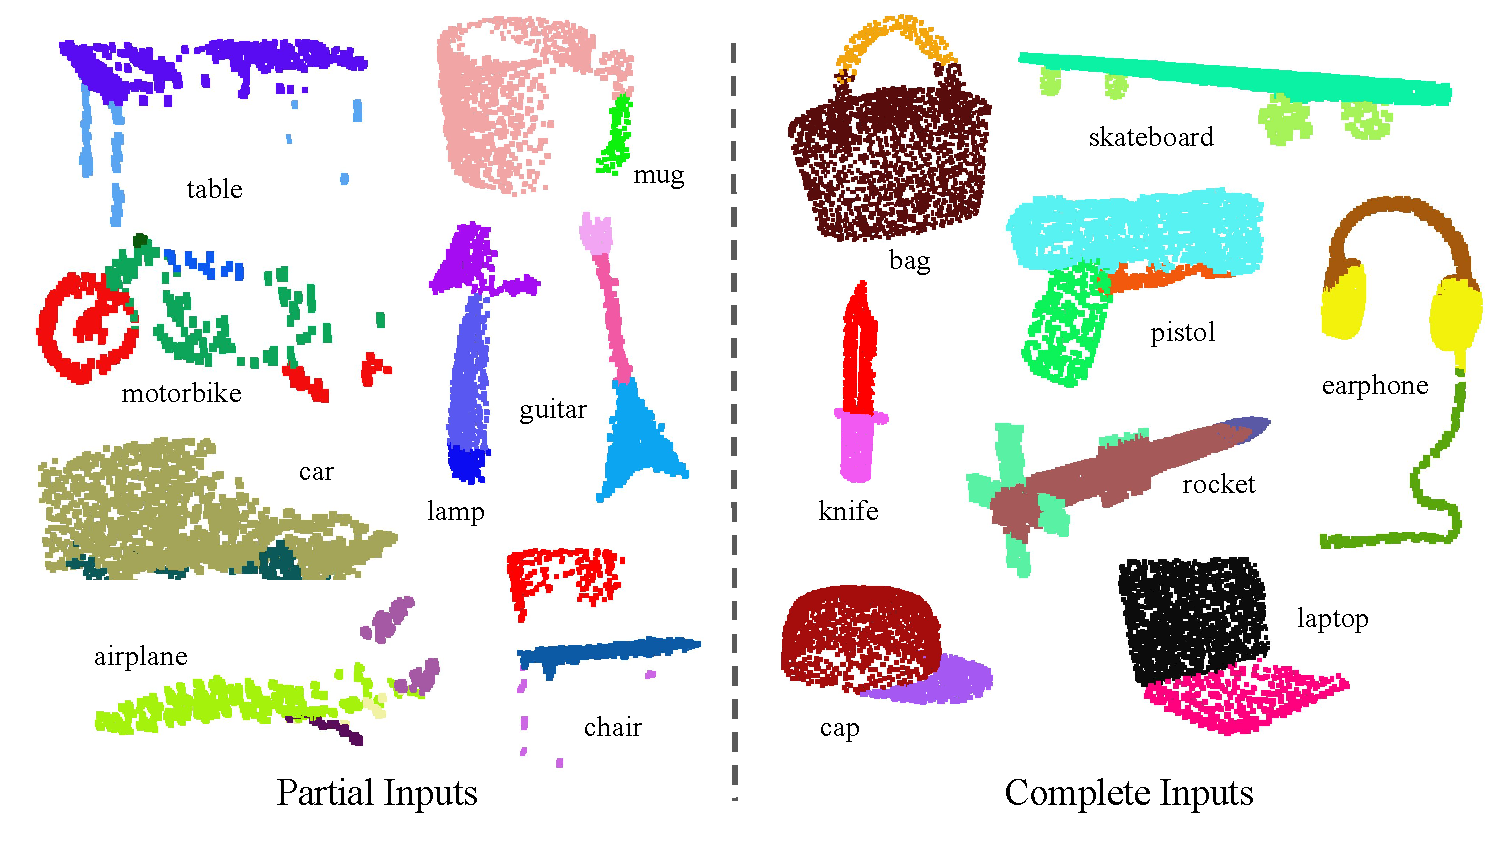
\includegraphics[width=0.8\linewidth]{fig/segres.pdf}
    \caption{
        \textbf{零件分割的量化结果} 我们可视化了横跨 16 个分类的 CAD 零件的分割结构。我们分别展示了部分模拟的 Kinect 扫描结果(左)和完全的 ShapeNet CAD 模型的结果(右)。
  %  \textbf{Qualitative results for part segmentation.} We visualize the CAD part segmentation results across all 16 object categories. We show both results for partial simulated Kinect scans (left block) and complete ShapeNet CAD models (right block).
    }
    \label{fig:qualitative_part_segmentation}
\end{figure}

\paragraph{瓶颈维度与稳定性} 从理论上和实践上,我们发现我们网络的表达性收到池化层维度的强烈影响。即,\eqref{eq:approx} 中的 $K$。在此我们提供了一个分析,同时也揭示了与我们模型的稳定性相关的一些属性。  

% \paragraph{Bottlenet dimension and stability} Theoretically and experimentally we find that the expressiveness of our network is strongly affected by the dimension of the max pooling layer, i.e., $K$ in \eqref{eq:approx}. Here we provide an analysis, which also reveals properties related to the stability of our model. 

我们定义 $\myvec u=\underset{x_i\in S}{\mbox{MAX}}\{h(x_i)\}$ 为网络 $f$ 的子网络。其中 $f$ 将分布在  $[0,1]^m$ 中的点集映射到了 $K$ 维空间的向量。接下来的理论分析指出,输入中的微小扰动或额外的噪音点不会严重影响我们网络的输出结果。

%We define $\myvec u=\underset{x_i\in S}{\mbox{MAX}}\{h(x_i)\}$ to be the sub-network of $f$ which maps a point set in $[0,1]^m$ to a $K$-dimensional vector. The following theorem tells us that small corruptions or extra noise points in the input set are not likely to change the output of our network:

\begin{theorem}

令 $\myvec u:\mathcal{X}\rightarrow \mathbb{R}^K$ 使得 $\myvec u=\underset{x_i\in S}{\mbox{MAX}}\{h(x_i)\}$ 且 $f=\gamma \circ \myvec u$. 则, 

% Suppose $\myvec u:\mathcal{X}\rightarrow \mathbb{R}^K$ such that $\myvec u=\underset{x_i\in S}{\mbox{MAX}}\{h(x_i)\}$ and $f=\gamma \circ \myvec u$. Then, 

\begin{enumerate}[label=(\alph*)]   

    \item $\forall S, \exists~\mathcal{C}_S, \mathcal{N}_S\subseteq \mathcal{X}$,  $f(T)=f(S)$ if  $\mathcal{C}_S\subseteq T\subseteq \mathcal{N}_S$;
    %\item Define the equivalence relation $\sim$ as $S\sim S'$ if $\myvec u(S)=\myvec u(S')$, then $\mathcal{C}_S=\underset{S'\sim S}{\cap} S'$ and $\mathcal{N}_S=\underset{S'\sim S}{\cup} S'$.
    % \item Let $S\sim S'$ if $\myvec u(S)=\myvec u(S')$. $\mathcal{C}_S=\underset{S'\sim S}{\cap} S'$, $\mathcal{N}_S=\underset{S'\sim S}{\cup} S'$.
    \item $|\mathcal{C}_S| \le K$
\end{enumerate}
\label{thm:thm2}
%     \begin{itemize}            
%     \item Critical points.
%     \\$\mathbb{C}=\{x_i: \myvec u_j(S)=h_j(x_i) \mbox{ for some } 1\le j\le K\}\cap S$
%     \item Free-space points.
%     \\$\mathbb{F}=\{x_i: \myvec u_j(S)<h_j(x_i) \mbox{ for some } 1\le j\le K\}\cap S$
%     \item Non-critical points. 
%     \\$\mathbb{N}=\{x_i: \myvec u_j(S)>h_j(x_i) \mbox{ for some } 1\le j\le K\}\cap S$
% For any $S'$ such that  $\mathbb{C} \subseteq S' \subseteq \mathbb{C}\cup\mathbb{N}$, $\myvec u(S')\equiv \myvec u(S)$; for any $S'$ such that $S'\cap \mathbb{F}\neq \emptyset$, $\myvec u(S')\neq \myvec u(S)$.
%\end{itemize}
\end{theorem}

关于上述定理,我们进一步阐释其推论。(a) 说明 $f(S)$ 在针对输入干扰时保持不变,只要  $\mathcal{C}_S$ 中的点被保留。同时也不会受到在 $\mathcal{N}_S$ 以内的额外噪声点的影响。(b) 说明 $\mathcal{C}_S$ 只包含一些有限数量的点,取决于 \eqref{eq:approx} 中的 $K$。换句话说,$f(S)$ 事实上是完全由一个元素数量小于或等于 $K$ 的有限子集 $\mathcal{C}_S\subseteq S$决定的。因此,我们将 $\mathcal{C}_S$ 称为 $S$ 的 \emph{关键点集},将 $K$ 成为 $f$ 的 \emph{瓶颈维度}。

% We explain the implications of the theorem. (a) says that $f(S)$ is unchanged up to the input corruption if all points in $\mathcal{C}_S$ are preserved; it is also unchanged with extra noise points up to $\mathcal{N}_S$. (b) says that $\mathcal{C}_S$ only contains a bounded number of points, determined by $K$ in \eqref{eq:approx}. In other words, $f(S)$ is in fact totally determined by a finite subset $\mathcal{C}_S\subseteq S$ of less or equal to $K$ elements. We therefore call $\mathcal{C}_S$ the \emph{critical point set} of $S$ and $K$ the \emph{bottleneck dimension} of $f$. 

结合 $h$ 的连续性,我们的模型关于点的扰动、缺失或额外的噪声点的健壮性得以解释。其健壮性的提升类似于机器学习模型中的稀疏原则。\textbf{直观上看,我们的模型能够通过一个稀疏的关键点来概括出形状。}在实验部分,我们可以看到从一个物体骨架的关键点。

% Combined with the continuity of $h$, this explains the robustness of our model w.r.t point perturbation, corruption and extra noise points. The robustness is gained in analogy to the sparsity principle in machine learning models. {\bf  Intuitively, our network learns to summarize a shape by a sparse set of key points.} In experiment section we see that the key points form the skeleton of an object.




\begin{comment}
\subsection{The properties of point sets in $\R^n$}
\todo{
  our input is a subset of points from a Euclidean space. It has three main properties:
  \begin{itemize}
    \item as a set, points in it has no order; 
    \item the points are from a metric space. therefore, local structures from near points have to be characterized;
    \item as a geometric object, the learned representation of the point set should be invariant to certain transformations.
  \end{itemize}
  the above three properties of our input leads to the three key ideas of our network design. we explain one by one.
}
\subsection{Unordered point set as input}
\todo{
  \begin{itemize}
    \item three strategies exist: 1) sorting input into a canonical order; 2)  use RNN but train order-invariantly; 3) use a symmetric function to aggregate the information from each point. 
    \item theoretically and empirically argue that the first two choices are not good. 
    \item our idea is to approximate a general function defined on a point set by applying a symmetric function on transformed elements in the set: $$f(\{x_1, \dots, x_n\})\approx g(h(x_1), \dots, h(x_n)),$$ where $f:2^{\R^N} \rightarrow \R$, $h: \R^N\rightarrow \R$ and $g:\R\times \dots \times \R\rightarrow \R$ is a symmetric function.
    \item we think this is provable for some good $f$.
    \item empirically, we approximate $h$ by a multi-layer perceptron network and $g$ by a composition of a single variable function and a max pooling function. this is found to work well by experiments.
    \item we can learn a number of $f$'s to capture different properties of the set.
  \end{itemize}
}

\subsection{Local and global information aggregation}
\todo{
  \begin{itemize}
    \item the output from the above section forms a vector $[f_1, \dots, f_M]$, which is a global signature of the input set.
    \item however, for tasks such as segmentation, we also need combine local information and global information. 
    \item xxx
  \end{itemize}
}

\subsection{Input and feature space alignment}
\todo{
  \begin{itemize}
    \item as we explained earlier, the learned representation of the point set should be invariant to certain transformations.
    \item we propose to apply an input dependent transformation for each instance to align all input set to a canonical space
    \item the input of our data are very friendly to geometric transformations, such as affine. we can therefore predict the transformation matrix by a neural network, named Joint Alignment Network.
    \item this idea can be extended to the alignment of feature space, as well
  \end{itemize} 
}

\subsection{PointNet architecture}
\todo{
  \begin{itemize}
    \item we implement the above ideas into a network for point set learning, named PointNet
    \item show the network for classification and explain 
    \item show the network for segmentation and explain
  \end{itemize}
}

\subsection{Theoretical Analysis}
\todo{
  goal: show that this network is theoretically robust to perturbation and corruption (additional points and incompleteness) of input data.
  \begin{itemize}
    \item analyze the max pooling layer: it selects a finite set of key points. the cardinality of the key point set is constrained by the dimension of max pooling. 
    \item add some understanding of the symmetry function, if we can
  \end{itemize}
}



\end{comment}

\section{实验}
\begin{table}[t!]
    \small
    \centering
    \begin{tabular}[width=\linewidth]{l|c|c|c|c}
    \hline
    ~               & input        & \#views    & accuracy & accuracy \\ 
    ~ & & & avg. class & overall \\ \hline
    SPH~\cite{kazhdan2003rotation}             & mesh        & - & 68.2         & -  \\ \hline
    3DShapeNets~\cite{wu20153d}     & volume       & 1        & 77.3  & 84.7 \\
    VoxNet~\cite{maturana2015voxnet}          & volume       & 12        & 83.0 & 85.9 \\
    Subvolume~\cite{qi2016volumetric}    & volume       & 20      & 86.0  & \textbf{89.2} \\ \hline
    LFD~\cite{wu20153d}             & image        & 10        & 75.5 & -\\
    MVCNN~\cite{su15mvcnn}           & image        & 80        & \textbf{90.1} & -\\ \hline
    Ours baseline  & point    & -     & 72.6  & 77.4\\
    Ours PointNet   & point   & 1        & 86.2 & \textbf{89.2} \\ \hline
    \end{tabular}
    \caption{\textbf{ModelNet40上的分类结果} 我们的网络在一系列3D输入的深度网络中达到最先进的效果。}
    \label{tab:classification}
\end{table}
\label{sec:exp}
实验被分成了四部分。首先,我们展示了PointNets可以应用于多个3D识别任务 (Sec~\ref{sec:application})。 其次,我们提供了详细的实验来验证我们的网络设计 (Sec~\ref{sec:arch_analysis})。最后,我们可视化了网络学到的内容 (Sec~\ref{sec:visualizing_pointnet}) 并且分析了时间和空间复杂度 (Sec~\ref{sec:complexity})。



\begin{table*}[th!]
    \small
    \centering
    \begin{tabular}[width=\linewidth]{l|c|p{0.5cm}p{0.4cm}p{0.4cm}p{0.4cm}p{0.5cm}p{0.6cm}p{0.5cm}p{0.5cm}p{0.5cm}p{0.6cm}p{0.6cm}p{0.3cm}p{0.5cm}p{0.6cm}p{0.6cm}p{0.6cm}}
    \hline
    ~        & mean & aero & bag & cap & car & chair & ear & guitar & knife & lamp & laptop & motor & mug & pistol & rocket & skate & table \\ 
    &   & &  &  &  &  & phone &  &   &  &  & &    &    &    & board &  \\ \hline
    \# shapes & & 2690 & 76 & 55 & 898 & 3758 & 69 & 787 & 392 & 1547 & 451 & 202 & 184 & 283 & 66 & 152 & 5271 \\ \hline
    Wu~\cite{Wu2014248} &  -  & 63.2  & - &      -    & -   & 73.5 & - &    - &    - &     74.4  & -    & - &   -   &   -   &   - & -  &  74.8 \\
    Yi~\cite{Yi16} & 81.4 & 81.0 & 78.4 & 77.7 & \textbf{75.7} & 87.6 & 61.9 & \textbf{92.0} & 85.4 & \textbf{82.5} & \textbf{95.7} & \textbf{70.6} & 91.9 & \textbf{85.9} & 53.1 & 69.8 & 75.3 \\ \hline
    3DCNN & 79.4 & 75.1 & 72.8 & 73.3 & 70.0 & 87.2 & 63.5 & 88.4 & 79.6 & 74.4 & 93.9 & 58.7 & 91.8 & 76.4 & 51.2 & 65.3 & 77.1 \\ 
    Ours & \textbf{83.7} & \textbf{83.4} & \textbf{78.7} & \textbf{82.5} & 74.9 & \textbf{89.6} & \textbf{73.0} & 91.5 & \textbf{85.9} & 80.8 & 95.3 & 65.2 & \textbf{93.0} & 81.2 & \textbf{57.9} & \textbf{72.8} & \textbf{80.6} \\ \hline
    \end{tabular}
    \caption{\textbf{ShapeNet数据集上的分割结果} 评价指标是点集的mIoU(\%)。 我们与两种传统方法 \cite{Wu2014248} \cite{Wu2014248} 以及我们提出的三维卷积网络对比。PointNet方法在mIoU上达到最佳表现。}
    %Notice that while all the other three methods are tested on the official ShapeNet train/validation/test split~\cite{shapenet2015}, the statistics for Wu's method~\cite{Wu2014248} are tested on a much larger set of shapes.
    \label{tab:segmentation}
\end{table*}



\subsection{应用}
\label{sec:application}
在本节中,我们将展示我们的网络是如何经过训练,来完成3D目标分类、目标零件分割和场景语义分割任务\footnote{更多应用样例,例如形状对应和基于点云的CAD模型检索包含在补充资料中。} 即使我们基于全新的数据表示(点集)进行研究,我们也能够在多个任务的基准测试中获得相当的甚至更好的性能。

\paragraph{3D目标分类} 我们的网络学习了可用于目标分类的全局点云特征。我们在ModelNet40~\cite{wu20153d} 形状分类基准上评估了我们的模型。总共有来自40个人造目标类别的12311个CAD模型,分为用于训练的9843个和用于测试的1468个。以前的方法主要集中于体积和多视图图像表示,我们提出了第一个直接处理原始点云的方法。

我们根据表面区域在网格面上均匀地采样了1024个点并将它们归一化为一个单位球体。在训练过程中,我们还通过沿上轴随机旋转对象并使用均值为0和标准差为0.02的高斯噪声抖动每个点的位置来动态地增强点云。


在表~\ref{tab:classification}中,我们将我们的模型与以前的相关工作,以及我们基于从点云中提取的传统特征(点密度、D2、形状轮廓等)MLP的基准线进行比较。我们的模型在基于3D输入(体积和点云)的所有方法中实现了最优的性能。仅仅使用全连接层和最大池化,我们的网络在推理速度上获得了强大的领先优势,并且也可以很容易地在CPU中并行化。但我们的方法与基于多视图的方法 (MVCNN~\cite{su15mvcnn}),之间仍然存在一点小差距,我们认为这是精细几何细节的丢失导致的,而这些细节可以被渲染图像所捕获。

\paragraph{3D目标零件分割} 零件分割是一项具有挑战性的细粒度3D识别任务。给定3D扫描或网格模型,任务是为每个点或面分配所属部分类别标签(例如椅子腿、杯柄)。
%The segmentation results are strong cues for part detection systems, which are key to many robotics applications such as grasping and affordance reasoning.

%Part segmentation requires knowledge of both local geometric and global semantics knowledge. By aggregating global feature vector to our point feature, our network is able to learn a \emph{deep point descriptor} that considers both local and global context, which suits well for this task.

我们对来自~\cite{Yi16}的ShapeNet部分数据集进行评估,其中包含来自16个类别的16881个形状,总共标注了50个部分。大多数目标类别都标有两到五个部分。对应的真实标签注释标记在形状上的采样点上。

我们将零件分割制定转换为每点分类问题。评估指标是点上的mIoU。对于类别C的每个形状S,计算形状的mIoU:对于类别C中的每个部分类型,计算真实和预测之间的IoU。如果真实点和预测点的并集为空,则将一部分IoU计为1。然后我们对类别C中所有部分类型的IoU进行平均以获得该形状的mIoU。为了计算类别的mIoU,我们取该类别中所有形状的mIoU的平均值。

在本节中,我们将我们的分割版PointNet (图~\ref{fig:pointnet_arch}的修改版, \textit{分割网络}) 和两种均利用了逐点几何特征和形状之间的对应关系的传统方法 \cite{Wu2014248} 和 \cite{Yi16} ,以及我们自有的3DCNN基准线进行了比较。有关3DCNN的详细修改和网络架构,请参阅补充说明。
%We design the segmentation 3D CNN architecture as a fully convolutional one that keeps volume size through all layers. In the end each voxel has a receptive field of 19 voxels with spatial resolution of 32.

在表~\ref{tab:segmentation}, 我们报告了每个类别和平均IoU(\%) 分数。我们观察到平均IoU有2.3\% 的提高,并且我们的网络在大多数类别中都优于基准方法。


\begin{table}[b!]
    \centering
    \small
    \begin{tabular}[width=\linewidth]{l|c|c}
    \hline
    ~             & mean IoU  & overall accuracy \\ \hline
    Ours baseline          &  20.12 & 53.19    \\ \hline
    Ours PointNet          & \textbf{47.71} & \textbf{78.62}  \\ \hline
    \end{tabular}
    \caption{\textbf{场景语义分割结果} 评价指标是13个类(结构和家具加上其他)的平均IoU和根据点集计算的分类准确率。 }
    \label{tab:semantic_segmentation}
\end{table}

\begin{table}[b!]
    \centering
    \small
    \begin{tabular}[width=\linewidth]{l|cccc|c}
    \hline
    ~                              & table & chair & sofa & board & mean  \\ \hline
    \# instance & 455 & 1363 & 55 & 137 & ~ \\ \hline
    Armeni et al.~\cite{armeni_cvpr16}          & 46.02 & 16.15 & \textbf{6.78} & 3.91  & 18.22 \\ \hline
    Ours & \textbf{46.67}     & \textbf{33.80 }    & 4.76    & \textbf{11.72}     & \textbf{24.24}     \\ \hline
    \end{tabular}
    \caption{\textbf{场景中3D物体检测结果} 评价指标是3D体积块中IoU阈值为0.5的平均准确率。}
    \label{tab:3d_detection}
\end{table}


% Move to supp
% While \cite{Wu2014248} and \cite{Yi16} deal with each object category independently, due to the lack of training data for some categories (the total number of shapes for all the categories in the data set are shown in the first line), we train our PointNet and the 3D volumetric CNN baseline across categories. To allow fair comparison, when testing these two models, we only predict part labels for the given specific object category. 

我们还对模拟Kinect扫描的任务进行了实验,来测试这些方法的稳健性。 对于ShapeNet部分数据集中的每个CAD模型,我们使用BlensorKinectSimulator~\cite{Gschwandtner11b} 从六个随机视点生成不完整的点云。我们根据这些完整形状和部分扫描数据,使用相同的网络架构和训练设置训练我们的PointNet。 结果表明,我们仅损失了5.3\%的平均IoU。 在图~\ref{fig:qualitative_part_segmentation}中,我们展示了针对完整数据和部分数据的定性结果。可以看到,虽然仅提供部分数据的任务相当具有挑战性,但我们的对其的预测是合理的。
%Since most real world scans are very partial due to occlusions, a model's robustness to partial input is key to evaluate its value in practice.


%From complete to partial input, we observed a $5.3\%$ mIoU drop. It is reasonable since lots of points are missed in virtual scans -- more structures need to be inferred. Still our model can segment well in some surprisingly partial cases, as shown in Fig~\ref{fig:qualitative_part_segmentation}, where both results on complete and partial data are displayed.

\begin{comment}
\begin{table}[h!]
    \small
    \centering
    \begin{tabular}[width=\linewidth]{l|cccc}
    \hline
    ~ & complete input & partial input \\ \hline
    3D CNN & 75.3 & 69.7 \\ \hline
    Ours PointNet & \textbf{80.6} & \textbf{75.3}  \\ \hline
    \end{tabular}
    \caption{\textbf{Segmentation results on partial scans.} Metric is mean IoU across all shapes.}
    %We perform rotation augmentation when training our PointNet on complete data to fairly compare with the simulated Kinect scans, that are generated from multiple perspective. In Table~\ref{tab:segmentation}, however, to compare with the traditional methods that rely on global orientation of shapes, no rotation augmentation is performed there.
    \label{tab:segmentation_partial}
\end{table}
\end{comment}

\paragraph{场景语义分割} 我们的零件分割网络可以很容易地扩展到语义场景分割,其中点标签成为语义目标类别,而不是目标的部分标签。
%Similar to image segmentation, we propose a 3D semantic segmentation task that organizes 3D points into semantic categories.

%Since our network operates on raw points, we can directly classify each point. On other hand, volumetric CNN and image based methods have to convert results back and forth in different representations.

% \begin{comment}
% Based on our net's ability to learn to classify 3D objects and segment point cloud, we can further achieve 3D object detection in scenes.
% \end{comment}

我们在斯坦福3D语义解析数据~\cite{armeni_cvpr16}上进行了实验。该数据集包含来自Matterport扫描仪的3D扫描结果,有6个大型室内区域组成,总共包括271个房间。扫描中的每个点都用来自13个类别(椅子、桌子、地板、墙壁等以及杂物)的语义标签中的一个进行注释。

为了准备训练数据,我们首先按房间分割点,然后将房间采样为面积为1mx1m的块。我们训练PointNet的分割版来预测每个块中的每个点类。每个点由XYZ、RGB和基于房间的归一化位置(从0到1)的9维向量表示。在训练时,我们实时的从每个块中随机采样4096个点。在测试时,我们对所有点进行测试。我们遵循与~\cite{armeni_cvpr16} 相同的协议,使用k-fold策略进行训练和测试。
%The sampled blocks have a overlap of half a meter. 


我们将我们的方法与使用人工设计点特征的基准线进行比较。基准线提取相同的9维局部特征和三个额外特征:局部点密度、局部曲率和法线。 我们使用标准MLP作为分类器。结果如表~\ref{tab:semantic_segmentation}所示,其中我们的PointNet方法明显优于基准线方法。 在图~\ref{fig:qualitative_segmentation}中,我们展示了定性分割结果。我们的网络能够输出平滑的预测,并且对缺失点和遮挡具有鲁棒性。




基于我们网络的语义分割输出,我们进一步构建了一个使用连接的组件进行目标采样的3D目标检测系统(有关详细信息,请参阅补充说明)。我们在表~\ref{tab:3d_detection}中与之前最先进的方法进行了比较。之前的方法基于滑动形状方法(带有CRF后处理),这种方法使用的支持向量机针对体素网格中的局部几何特征和全局房间上下文特征进行训练。我们的方法在所报告的家具类别上的效果大大优于它。

%we build a simple 3D object detection system. We use connected component with segmentation scores to get object proposals in scenes. For each proposed object, it's detection score is computed as the average point score for that category. Proposals with too less points or too small areas/volumes are pruned before evaluation. We observe that in some rooms such as auditoriums lots of objects (e.g. chairs) are close to each other, where connected component would fail to correctly segment out individual ones. Therefore we leverage our classification network and uses sliding shape method to alleviate the problem. The proposed boxes from connected component and sliding shapes are combined for final evaluation~\footnote{See supplementary for more details on implementation.}.



\begin{figure}[t!]
    \centering
    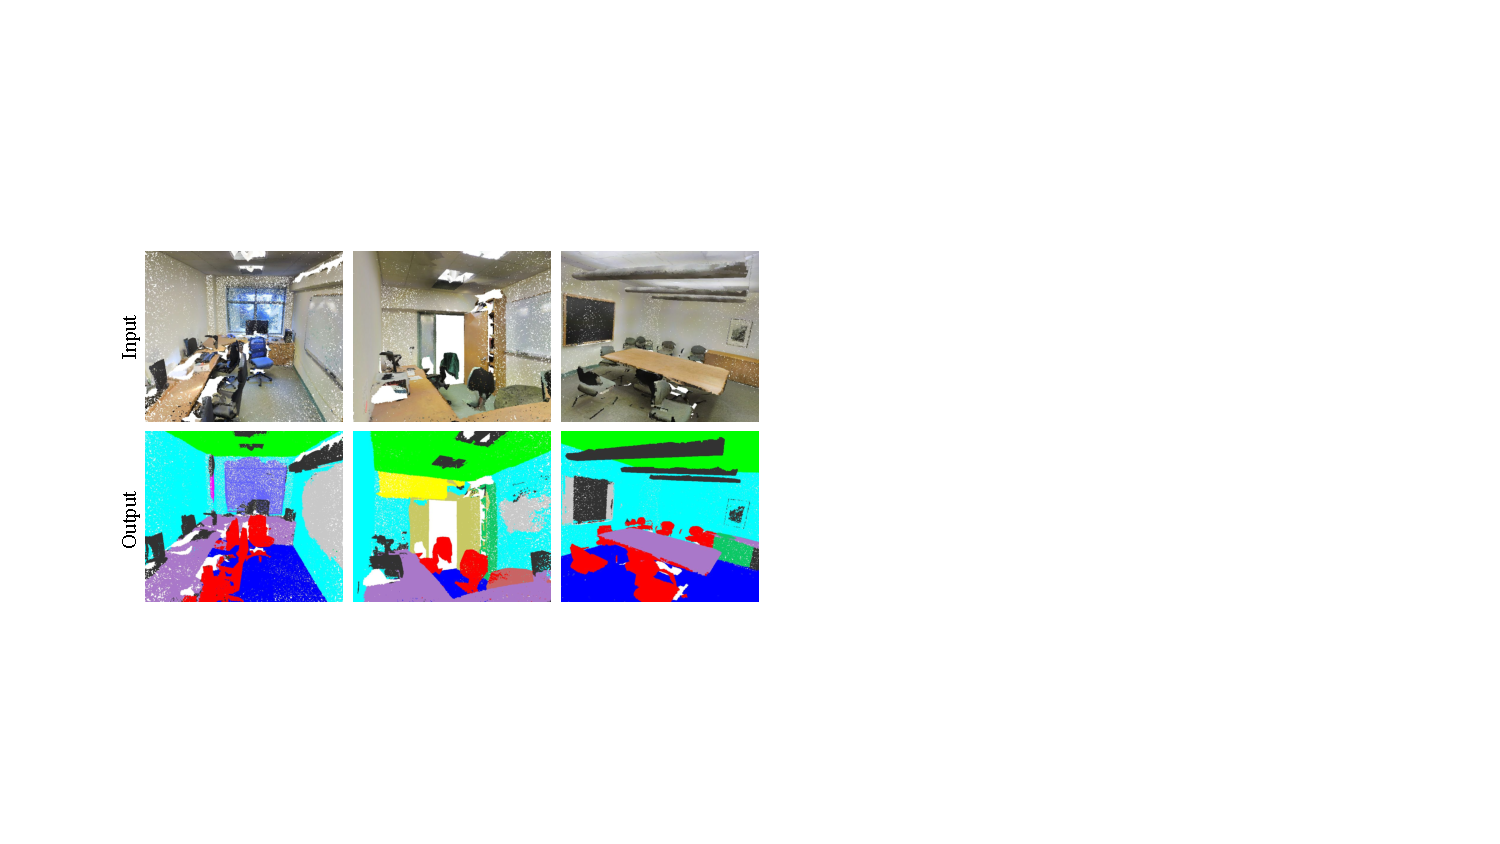
\includegraphics[width=0.8\linewidth,height=4cm]{fig/semantic}
    \caption{\textbf{语义分割的定性结果} 上一行是带颜色纹理的点云。底下是输出的语义分割结果(以点云展示),输出结果展示同输入的相机角度一致。}
    \label{fig:qualitative_segmentation}
\end{figure}

\subsection{架构设计分析}
\label{sec:arch_analysis}

在本节中,我们通过控制验证我们的设计选择实验。我们还展示了我们网络超参数的影响。
%~\footnote{Due to the limit of space, we refer the analysis on bottleneck dimension and number of input points to supplementary.}


\paragraph{与替代顺序不变方法的比较} 如第~\ref{sec:pointnet_arch}节所述,至少有三种选择可用于使用无序集合输入。我们使用ModelNet40形状分类问题作为测试平台来比较这些选项,以下两个控制实验也将使用此任务。

我们比较的基准线 (如图~\ref{fig:order_invariant}所示)包括:未排序和已排序的 $n \times 3$ 数组的多层感知机,将输入点视为序列的RNN模型,以及基于对称函数的模型。我们实验的对称操作包括最大池化、平均池化和基于注意力的加权和。注意方法类似于~\cite{vinyals2015order}中的方法,即从每个点特征预测一个标量分数,然后通过计算softmax跨点对分数进行归一化。然后根据归一化分数和点特征计算加权和。如图~\ref{fig:order_invariant}所示,最大池化操作以较大的优势幅度实现了最佳性能,这验证了我们的选择。


% \begin{table}
%     \small
%     \centering
%     \begin{tabular}[width=\linewidth]{l|c}
%     \hline
%     ~                    & accuracy \\ \hline
%     MLP (unsorted input) & 24.2       \\
%     MLP (sorted input)   & 45.0       \\
%     LSTM                 & 78.5       \\ \hline
%     Attention sum        & 83.0       \\
%     Average pooling      & 83.8       \\
%     Max pooling          & \textbf{87.1}       \\ \hline
%     \end{tabular}
%     \caption{\textbf{Comparing different order invariant methods.} Metric is classification overall accuracy on ModelNet40 test set. Max pooling is performing surprisingly well.}
%     \label{tab:order_invariant}
% \end{table}

\begin{figure}[t!]
    \centering
    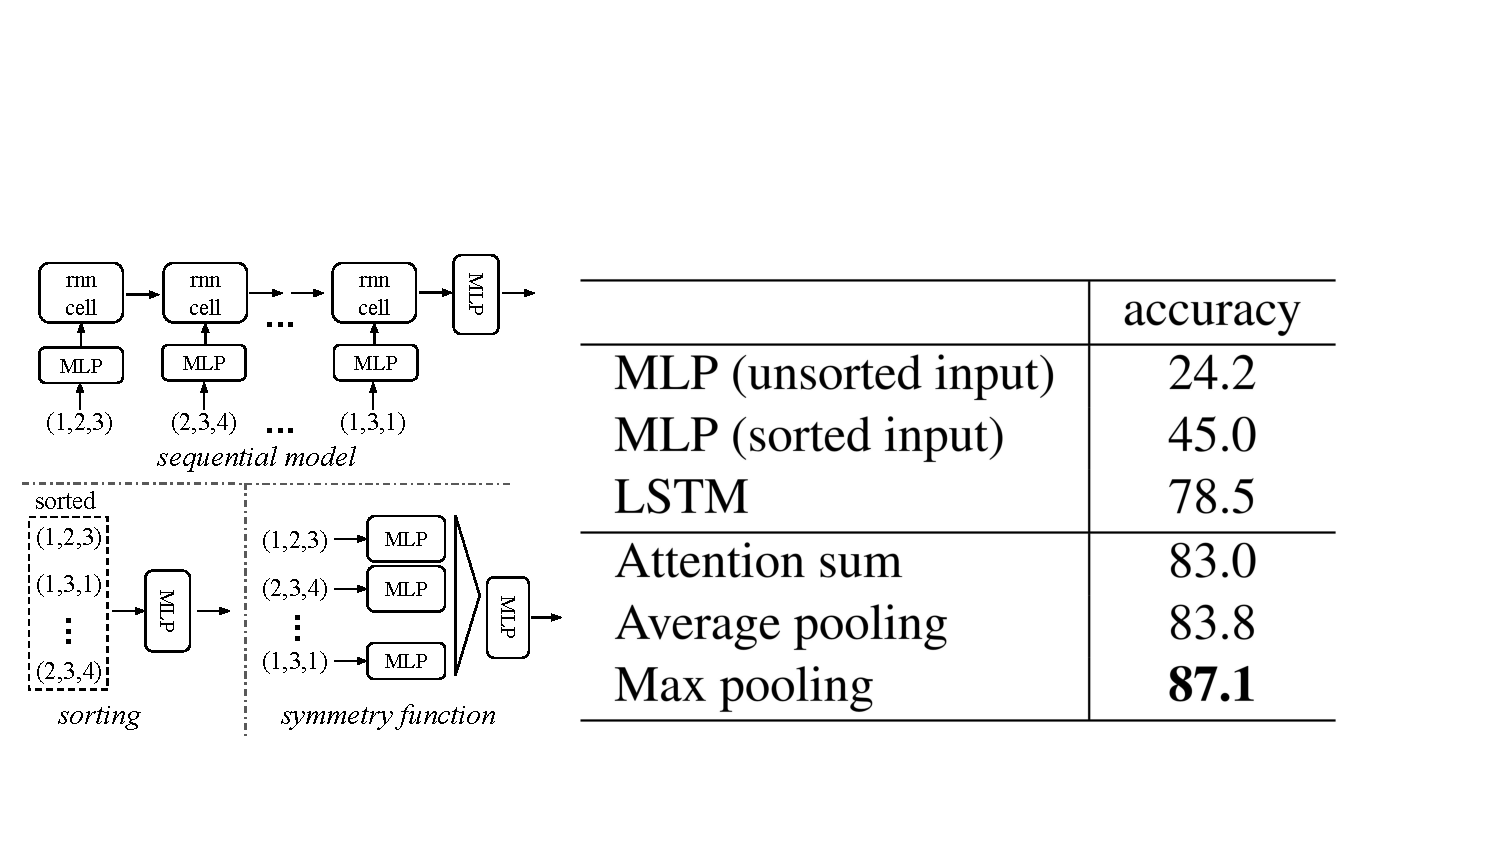
\includegraphics[width=\linewidth]{fig/order_invariant2.pdf}
    \caption{\textbf{三种实现顺序不变性的方法}神经元尺寸为64,64,64,128,1024,的5层隐藏层的多层感知机(MLP)应用在点集上,所有点共享一个简单的MLP副本。靠近输出的MLP共有两层,尺寸为512,256。}
    \label{fig:order_invariant}
\end{figure}

\paragraph{输入和特征转换的有效性} 在表~\ref{tab:transform}中,我们展示了我们的输入和特征转换(用于对齐)的积极影响。有趣的是,最基本的架构已经取得了相当合理的结果。使用输入转换可提高 $0.8\%$ 的性能。正则化损失是高维变换起作用所必需的。通过结合转换和正则化项,我们实现了最佳性能。

\begin{table}[b!]
    \small
    \centering
    \begin{tabular}[width=\linewidth]{l|c}
    \hline
    Transform              & accuracy \\ \hline
    none                   & 87.1     \\ \hline
    input (3x3)            & 87.9     \\
    feature (64x64)        & 86.9     \\
    feature (64x64) + reg. & 87.4     \\ \hline
    both                   & \textbf{89.2}     \\ \hline
    \end{tabular}
    \caption{\textbf{输入特征转换的效果} 评价指标是ModelNet40测试集上的总体分类准确率}
    \label{tab:transform}
\end{table}


% \paragraph{Effects of Max Layer Size and Number of Points} Here we show our model's performance change with regard to the size of the first max layer output as well as the number of input points. In Fig~\ref{fig:net_param} we see that performance grows as we increase the number of points however it saturates at around 1K points. The max layer size plays an important role, increasing the layer size from 64 to 1024 results in a $2-4\%$ performance gain. It indicates that we need enough point feature functions to cover the 3D space in order to discriminate different shapes.

% \begin{figure}
%     \centering
%     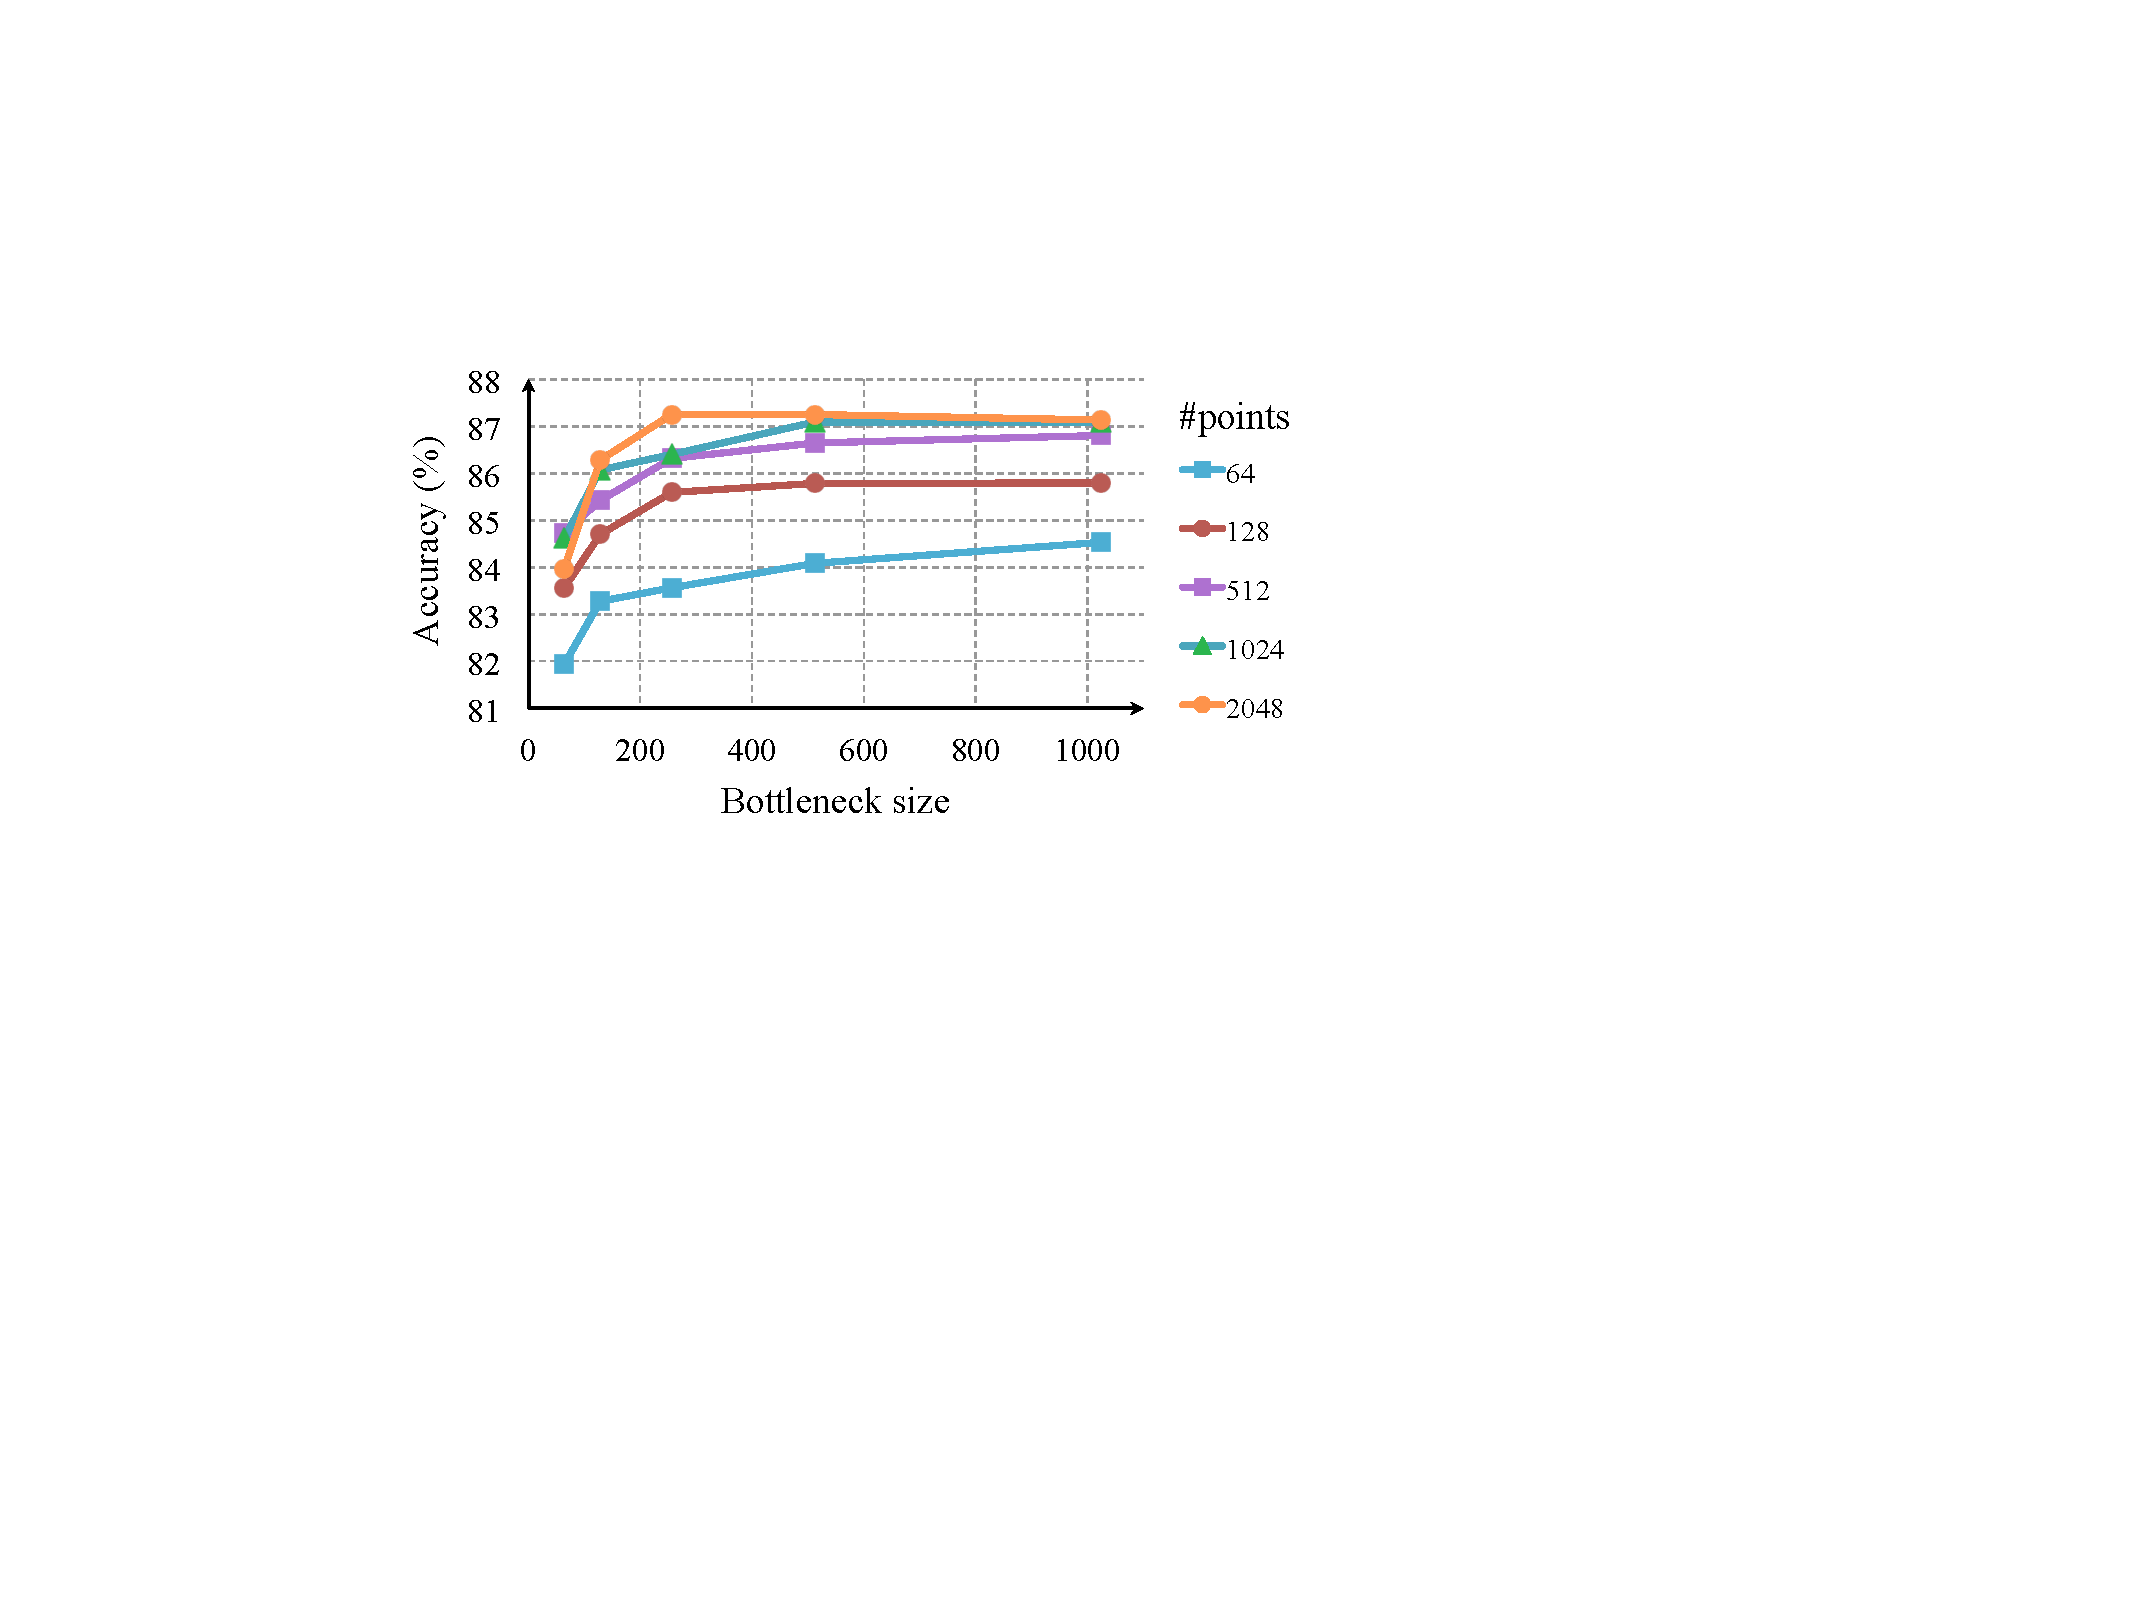
\includegraphics[width=0.8\linewidth]{fig/bottleneck.pdf}
%     \caption{\textbf{Effects of bottleneck size and number of input points.} The metric is overall classification accuracy on ModelNet40 test set.}
%     \label{fig:net_param}
% \end{figure}

\paragraph{鲁棒性测试} 我们展示了我们的PointNet不仅简单有效,还对各种输入损坏具有鲁棒性。我们使用与图~\ref{fig:order_invariant}的最大池化网络相同的架构。输入点被归一化为一个单位球体。结果如图~\ref{fig:robustness}。

A对于缺失点,当有 $50\%$ 的点缺失时,准确率仅下降 $2.4\%$ ,并且对于最远和随机输入采样则是 $3.8\%$ 。我们的网络在训练期间看到了异常点你,那么它对异常点也具有鲁棒性,。我们评估了两种模型:一种在具有 $(x,y,z)$ 坐标的点上进行训练;另一个在 $(x,y,z)$ 上加上点密度。即使当 $20\%$ 的点是异常值,网络也有超过 $80\%$ 的准确率。图~\ref{fig:robustness}右侧显示了网络对点扰动的鲁棒性。

\begin{figure}
    \centering
    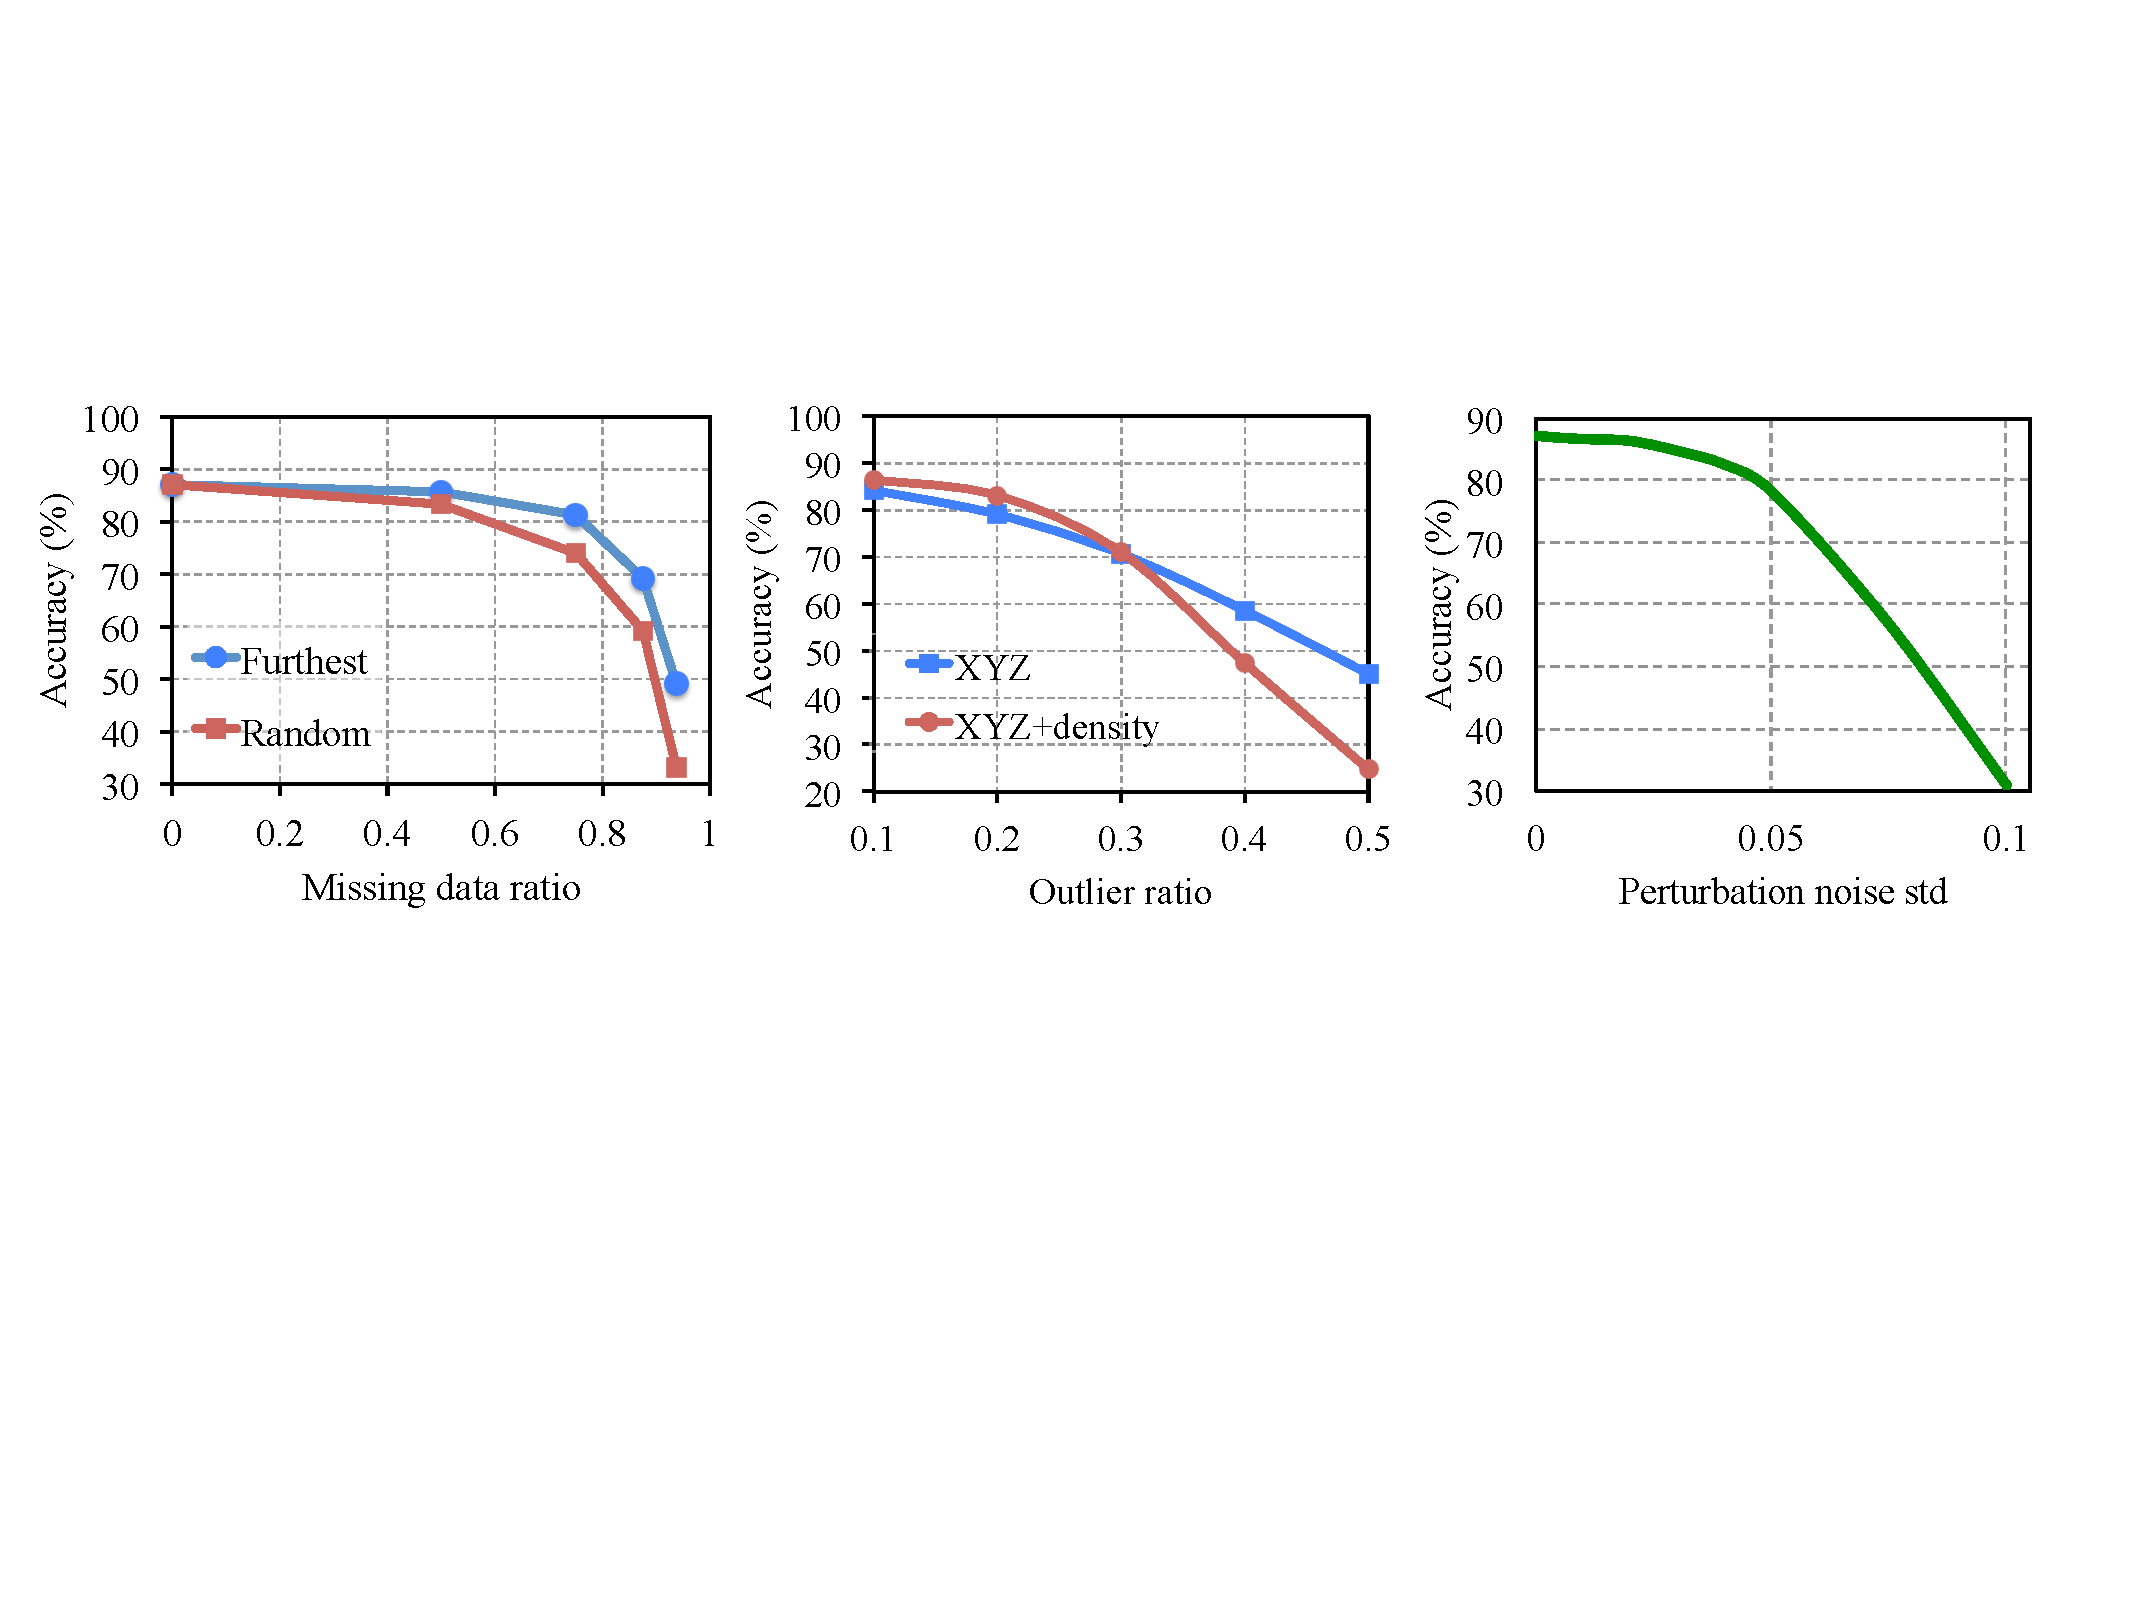
\includegraphics[width=\linewidth]{fig/robustness.pdf}
    \caption{\textbf{PointNet鲁棒性测试} 评价指标是ModelNet40测试集上的总体分类准确率。 左侧: 删除点的情况 Furthest意思是对1024个原始点采用最远点采样。 中间: 离群点插入的情况。离群点均匀的分布在单位球体中。 右侧: 点扰动的情况。单独对每个点进行高斯噪声扰动}
    \label{fig:robustness}
\end{figure}

\begin{comment}
\paragraph{MNIST Digit Classification} While we focus on 3D point cloud learning, a sanity check experiment is to apply our network on a 2D point clouds - pixel sets.

To convert an MNIST image into a 2D point set we threshold pixel values and add the pixel (represented as a point with XY coordinate in the image) with values larger than 128 to the set. We use a set size of 256. If there are more than 256 pixels int he set, we randomly subsample it; if there are less, we pad the set with the one of the pixels in the set (due to our max operation, which point used for the padding will not affect outcome). 
3
As seen in Table~\ref{tab:mnist}, we compare with a few baselines including multi-layer perceptron that considers input image as an ordered vector, a RNN that consider input as sequence from pixel (0,0) to pixel (27,27), and a vanila CNN. It's interesting to see that our model can achieve quite good performance by considering the image as a 2D point set.

% vanila CNN: https://www.microsoft.com/en-us/research/publication/best-practices-for-convolutional-neural-networks-applied-to-visual-document-analysis/
\begin{table}[h!]
    \centering
    \begin{tabular}[width=\linewidth]{l|c|c}
    \hline
    ~                      & input & error (\%) \\ \hline
    Multi-layer perceptron~\cite{simard2003best} & vector & 1.60  \\
    LeNet5~\cite{lecun1998gradient}                 & image & 0.80 \\ \hline
    Ours PointNet          & point set & 0.78 \\ \hline
    \end{tabular}
    \caption{\textbf{MNIST classification results.} We compare with vanila versions of other deep architectures to show that our network based on point sets input is achieving reasonable performance on this traditional task.}
    \label{tab:mnist}
\end{table}
\end{comment}


% \begin{figure}[b!]
%     \centering
%     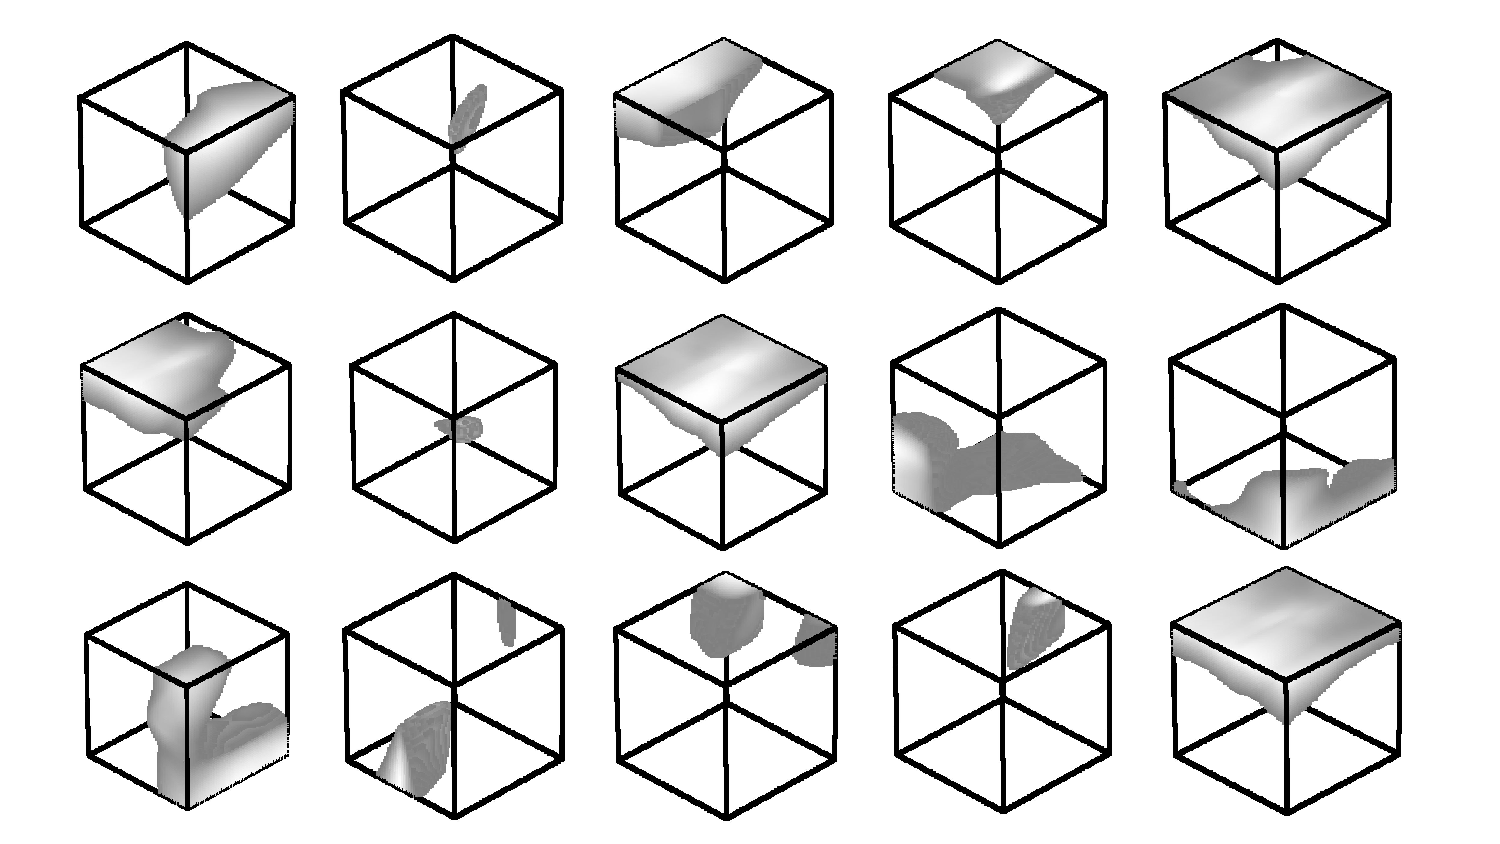
\includegraphics[width=0.7\linewidth]{fig/kernels.pdf}
%     \caption{\textbf{Point function visualization.} For each per-point function $h$, we calculate the values $h(p)$ for all the points $p$ in a cube of diameter two located at the origin, which spatially covers the unit sphere to which our input shapes are normalized when training our PointNet. In this figure, we visualize all the points $p$ that give $h(p)>0.5$ with function values color-coded by the brightness of the voxel. We randomly pick 15 point functions and visualize the activation regions for them.}
%     \label{fig:functions}
% \end{figure}


\subsection{可视化PointNet}
\label{sec:visualizing_pointnet}
% We design two experiments to visualize what has been learnt by the PointNet. The results are consistent with the theoretical analysis in Sec~\ref{sec:theory}. In the first experiment, we visualize the learnt point function $h(x)$ in Eq~\ref{eq:approx}, which demonstrates that our network learns a family of optimization criteria that selects informative points from the cloud. Our second experiment illustrates the robustness of our network, as explained in Thm~\ref{thm:thm2}.

% \paragraph{Point Function Visualization} As discussed in Sec~\ref{sec:pointnet_arch}, our network computes $K$ (we take $K=1024$ in this experiment) dimension point features for each point and aggregates all the per-point local features via a max pooling layer into a single $K$-dim vector, which forms the global shape descriptor. 

% To gain more insights on what the learnt per-point functions $h$'s detect, we visualize the points $p_i$'s that give high per-point function value $f(p_i)$ in Fig~\ref{fig:functions}. This visualization clearly shows that different point functions learn to detect for points in different regions with various shapes scattered in the whole space. 

\begin{comment}
This visualization is similar to the kernel visualization in convolutional neural networks in the sense that we'd like to know what input patterns would activate a specific neuron. However, our point function is behaving in a very differnt way from conv kernels.
\end{comment}

在图~\ref{fig:recon},我们可视化了一些样本形状 $S$ 的 \textit{关键点集} $\mathcal{C}_S$ 和 \textit{上边界形状} $\mathcal{N}_S$ (如Thm~\ref{thm:thm2}所述)。两个形状之间的点集将给出完全相同的全局形状特征 $f(S)$。

从图~\ref{fig:recon} 可以清楚地看出, \textit{关键点集} $\mathcal{C}_S$中对最大池化特征有贡献的点,总结了形状的主干。
%, or sample a sparse collection of points to describe the geometry of the whole shape.
\textit{上界形状} $\mathcal{N}_S$ 说明了与输入点云 $S$ 具有相同全局形状特征 $f(S)$ 的最大可能点云。$\mathcal{C}_S$ 和 $\mathcal{N}_S$反映了PointNet的鲁棒性,这意味着丢失一些非关键点不会改变全局形状特征 $f(S)$。



% We visualize the shape family, as discussed in Thm~\ref{thm:thm2}, including all the shapes between the \textit{critical point set} $\mathcal{C}_S$ and the \textit{upper-bound shape} $\mathcal{N}_S$ that gives the same global feature $f(S)$ with respect to a given shape $S$.

\begin{figure}[b]
    \centering
    % \includegraphics[width=0.8\linewidth]{fig/recon.pdf}
    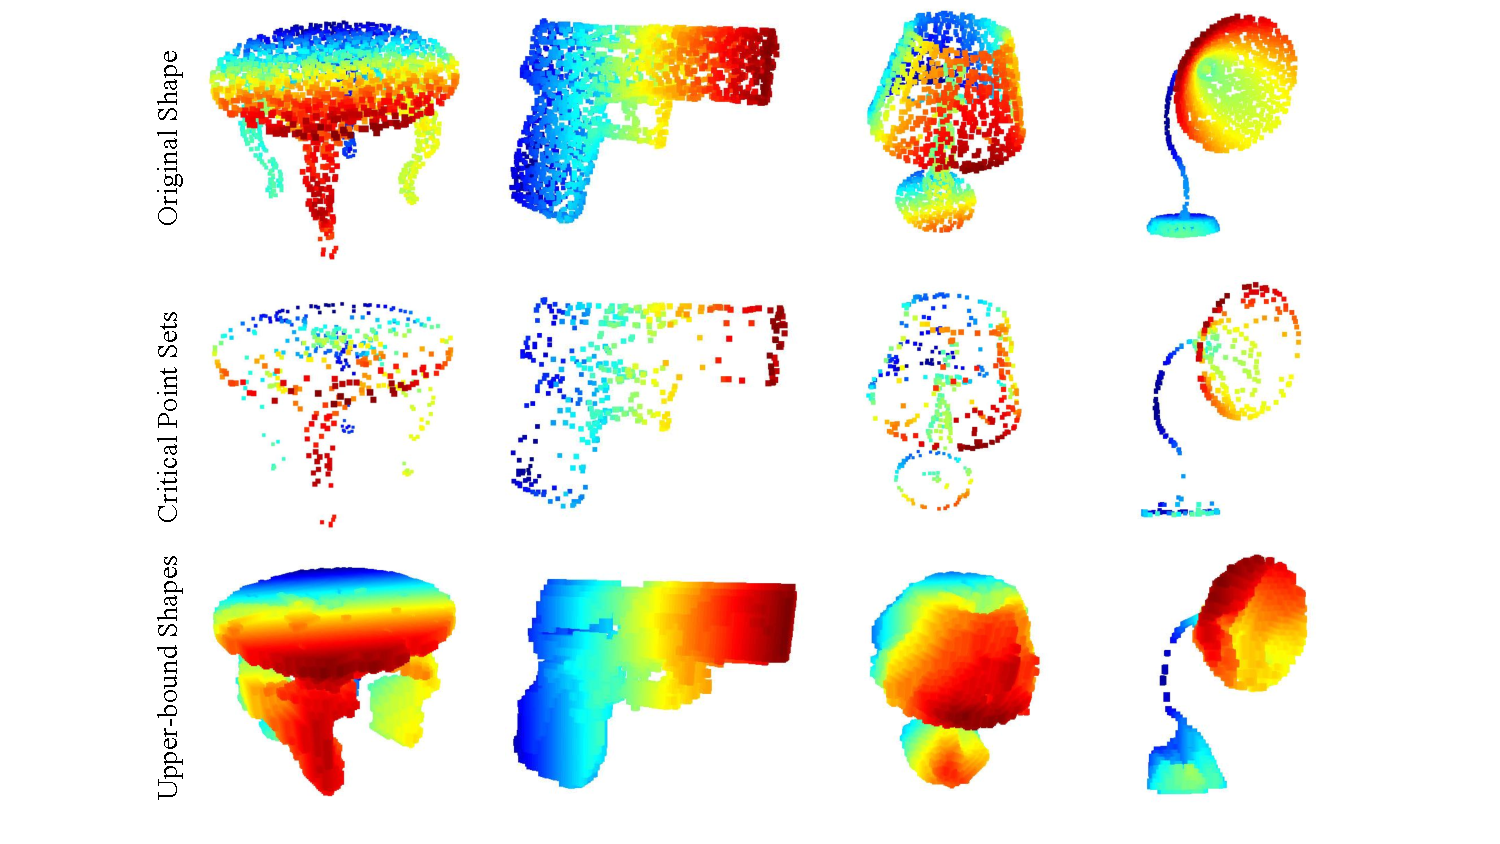
\includegraphics[width=0.8\linewidth]{fig/kp_ss_visu1.pdf}
    \caption{\textbf{关键点集和上界形状} 关键点集和上界形状共同决定了给定形状的全局形状特征,任何处于关键点集和上界形状间的点云都有同样一致的特征。 我们通过色彩编码来体现物体的深度信息。}
    \label{fig:recon}
\end{figure}

% Fig~\ref{fig:recon} shows the \textit{critical point sets} $\mathcal{C}_S$ and \textit{upper-bound shapes} $\mathcal{N}_S$ for four selected shapes. 
%The original input point clouds are rendered in the first row while the $\mathcal{C}_S$ and $\mathcal{N}_S$ for them are shown in the second and their rows respectively.
%The $\mathcal{C}_S$ for a given shape $S$ includes the points from the original point cloud that activates some point function $h_i$'s the most. 
$\mathcal{N}_S$ 是通过将边长为2的立方体中的所有点经过网络前向传播后,选择点函数值$(h_1(p), h_2(p), \cdots, h_K(p))$ 不大于全局形状描述符的点 $p$ 来构建的。
% It is not hard to see that all the shapes $S'$ that cover $\mathcal{C}_S$ and are contained by $\mathcal{N}_S$ give the exactly same global feature $f(S')=f(S)$. The transition shape family entails the robustness of the our PointNet, meaning that adding noisy jitterings or losing some non-critical points do not change the learnt shape signature and thus do not affect our classification or segmentation results.

\begin{comment}
We start from a max pooled vector of a specific input point cloud $X$, and find a set of point cloud $S$ (it's a set of point sets) where each point cloud in the set $S$ will result in the same max pooled vector as to $X$. In another word, we will reconstruct the input with only the knowledge of $X$ and the network parameters.

Assuming when feeding input point cloud $X$ to the network the first max-pooling layer's output is $g(X) = MAX\{f(x_1), f(x_2), ..., f(x_N)\} \in \R^{1024}$, where $X = \{x_1, x_2, ..., x_N\}$. We achieve the reconstruction by firstly construct a dense volumetric grids. Each voxel represents a point in 3D space. Then we will sweep through each point $p$ in the volume and judge whether this point's feature $f(p) \in \R^{1024}$ has any value larger than that in the corresponding dimension of $g(X)$. If there is , it means the point $p$ cannot be the input that results in $g(X)$, so we will exclude this point. After sweeping the volume, all the points left are possible to be part of the input set $X$. This set of points forms a upper bound of any possible input set that gets max pooling outcome of $g(X)$. Some reconstructed results of this upper bound is visualized in the second row of Fig~\ref{fig:recon}.

On the other hand, if we know the input set (set $X$) and the network, we can know which input points (subset $Y$ of $X$) are actually contributing to the final value of the max pooled vector. Excluding all the points in $X \\ Y$ will not affect the result. We call this contributing set of points the lower bound of the input, as visualized in the third row of Fig~\ref{fig:recon}. Any point sets that fall between the lower bound and upper bound will result in exactly the same result.
\end{comment}





\subsection{时间和空间复杂度分析}
\label{sec:complexity}
表~\ref{pointnet_complexity} 总结了我们PointNet分类网络的空间(网络中的参数个数)和时间(浮点运算/样本)复杂性。我们还将PointNet与之前工作中的一组具有代表性的基于体积和多视图的架构进行了比较。

尽管MVCNN~\cite{su15mvcnn} 和Subvolume (3D CNN) ~\cite{qi2016volumetric} 实现了高性能,PointNet的计算成本更低,效率更高(以FLOPs/样本衡量:效率分别提高\emph{141倍} 和 \emph{8倍})。此外,就网络中的\#param(参数少\emph{17倍})而言,PointNet的空间效率比MVCNN高得多。此外,PointNet更具可扩展性——它的空间和时间复杂度为 $O(N)$ —— 与输入点的数量呈\emph{线性} 关系。然而,由于卷积占用计算时间,多视图方法的时间复杂度随图像分辨率\emph{平方级}增长,基于体积卷积的方法随着体积大小成\emph{立方级}增长。

根据经验,PointNet能够处理超过每秒100万个点用于点云分类(约1K对象/秒)或语义分割(约2个房间/秒),在TensorFlow上使用1080XGPU,显示出实时应用的巨大潜力。

\begin{table}[h!]
    \centering
    \begin{tabular}{|l|l|l|l|}
    \hline
    ~                & \#params & FLOPs/sample\\ \hline
    PointNet (vanilla)  & 0.8M                        & 148M \\
    PointNet         & 3.5M                         & 440M \\ \hline
    %VoxNet~\cite{maturana2015voxnet}           & 0.07M                        & 204M \\
    Subvolume~\cite{qi2016volumetric} & 16.6M                        & 3633M \\ \hline
    MVCNN~\cite{su15mvcnn}   & 60.0M                          & 62057M \\ \hline
    \end{tabular}
    \caption{\textbf{处理3D数据分类的深度学习架构的时间和空间复杂度} PointNet (vanilla) 是分类版的PointNet除去输入和特征转化部分的版本。 FLOP代表浮点运算操作。
    ``M'' 代表百万。 Subvolume和MVCNN都使用了多次旋转和多个视角池化后的数据,没有这些操作他们的表现会大大下降}
    \label{pointnet_complexity}
    \vspace{-3mm}
\end{table}

\section{结论}
\label{sec:conclusion}
在这项工作中,我们提出了一种新颖的、可以直接使用点云输入的深度神经网络 \emph{PointNet} 。我们的网络为许多3D识别任务提供了统一的方法,这些3D识别任务包括目标分类、零件分割和语义分割,同时在标准基准上获得与现有技术相当或更好的结果。我们还提供理论分析和可视化来理解我们的网络。



\mypara{致谢} 作者非常感谢三星GRO授予的资助、ONR MURI N00014-13-1-0341的资助、NSF授予资助IIS-1528025、Google重点研究奖、来自Adobe公司的礼物和NVIDIA的硬件捐赠的支持。

{\small

\begin{thebibliography}{}
\documentclass[10pt,twocolumn,letterpaper,UTF8]{article}
\hyphenpenalty=2000
\textwidth=6.5in
\textheight=9.0in
\evensidemargin=0.0in
\oddsidemargin=0.0in
\topmargin=-0.5in
\clubpenalty=4000
\widowpenalty=4000
\displaywidowpenalty=500

\newlength\minalignvsep

\usepackage{cvpr}
\usepackage{times}
\usepackage{epsfig}
\usepackage{graphicx}
\usepackage{amsmath,amssymb,amsthm}
\usepackage{pbox}
\usepackage{epstopdf}
\usepackage{subfigure}
\usepackage{xspace}
\usepackage{comment}
\usepackage{lipsum}
%\usepackage{jeffe}
\usepackage{enumitem}

% 中文支持
\usepackage{ctex}
\usepackage[T1]{fontenc}
\usepackage{mathpazo}
\usepackage{fontspec}
\setmainfont[Scale = 1]{TeX Gyre Pagella}
\setCJKmainfont[ItalicFont=Noto Serif CJK SC Bold, BoldFont=Noto Serif CJK SC Black, Scale = 1]{Noto Serif CJK SC}

\newcommand{\cmt}[2]{[#1: #2]}
\newcommand{\todo}[1]{\cmt{{\bf TODO}}{{\bf \color{red} #1}}}
\newcommand{\hao}[1]{\cmt{{\bf Hao}}{{\bf \color{red} #1}}}
\newcommand{\rqi}[1]{\cmt{{\bf Charles}}{{\bf \color{blue} #1}}}
\newcommand{\km}[1]{\cmt{{\bf Kaichun}}{{\bf \color{green} #1}}}
\newcommand{\leo}[1]{\cmt{{\bf Leo}}{{\bf \color{cyan} #1}}}

\newcommand{\shape}{S}
\newcommand{\image}{I}
\newcommand{\network}{\mathbb{G}}
\newcommand{\prob}{\mathcal{P}}

\newcommand{\para}[1]{\noindent{\bf #1}}

\newcommand{\softpara}{\paragraph}
\newcommand{\mypara}{\vspace*{-15pt}\paragraph}

\newcommand{\bmemo}[1]{\noindent{\color{blue}{\sf [[#1]]}}}

\newcommand{\denselist}{\itemsep 0pt\parsep=0pt\partopsep 0pt\vspace{-2pt}}
\newcommand{\bitem}{\begin{itemize}\denselist}
\newcommand{\eitem}{\end{itemize}}
\newcommand{\benum}{\begin{enumerate}\denselist}
\newcommand{\eenum}{\end{enumerate}}
\newcommand{\bdescr}{\begin{description}\denselist}
\newcommand{\edescr}{\end{description}}

\newcommand{\Remark}[1]     {{\sf [#1]}}

\setlength{\abovedisplayskip}{0pt}
\setlength{\belowdisplayskip}{0pt}

\newtheorem{theorem}{Theorem}

\newcommand{\myvec}[1]{\mathbf #1}
\newcommand\blfootnote[1]{%
  \begingroup
  \renewcommand\thefootnote{}\footnote{#1}%
  \addtocounter{footnote}{-1}%
  \endgroup
}
\newtheorem{innercustomthm}{Theorem}
\newenvironment{customthm}[1]
  {\renewcommand\theinnercustomthm{#1}\innercustomthm}
  {\endinnercustomthm}
  
% Include other packages here, before hyperref.

% If you comment hyperref and then uncomment it, you should delete
% egpaper.aux before re-running latex.  (Or just hit 'q' on the first latex
% run, let it finish, and you should be clear).
\usepackage[pagebackref=true,breaklinks=true,letterpaper=true,colorlinks,bookmarks=false]{hyperref}

\cvprfinalcopy % *** Uncomment this line for the final submission

\def\cvprPaperID{201} % *** Enter the CVPR Paper ID here
\def\httilde{\mbox{\tt\raisebox{-.5ex}{\symbol{126}}}}

% Pages are numbered in submission mode, and unnumbered in camera-ready
\ifcvprfinal\pagestyle{empty}\fi
\begin{document}

%%%%%%%%% TITLE
\title{PointNet: 针对三维分类点云分类与分割的深度学习模型
% PointNet: Deep Learning on Point Sets for 3D Classification and Segmentation
}

% \author{First Author\\
% Institution1\\
% Institution1 address\\
% {\tt\small firstauthor@i1.org}
% % For a paper whose authors are all at the same institution,
% % omit the following lines up until the closing ``}''.
% % Additional authors and addresses can be added with ``\and'',
% % just like the second author.
% % To save space, use either the email address or home page, not both
% \and
% Second Author\\
% Institution2\\
% First line of institution2 address\\
% {\tt\small secondauthor@i2.org}
% }

\author{Charles R. Qi*\qquad Hao Su* \qquad Kaichun Mo \qquad Leonidas J. Guibas\\Stanford University\\翻译: 浙江大学软件学院 2021 年夏令营 CAD 第三小组}

\maketitle
%\thispagestyle{empty}

%%%%%%%%% ABSTRACT
\begin{abstract}
{\normalfont
  % - input is very special, other people do qualization, have problem
% - we directly consume point set by unified architecture, for object classication, part seg, and scene seg
% - our network is simple. it respects the permutuation inv by max pooling. 
% - the method is very effective, supported by theoretical analysis and experimental evidences.

点云是一种重要的几何数据结构。由于其无序性,大多数研究者将这些数据转换为有序的三维体素网格或图像集合。然而,这会导致不必要的数据冗余并引起一些问题。在本文中,我们设计了一种直接处理点云的新型神经网络,这种网络很好的考虑了输入中的点的置换不变性。我们构建了名叫PointNet的神经网络,它为物体分类、零件分割和场景语义分析等应用程序提供了统一的结构。PointNet结构虽然简单,但却十分高效且有效。从经验上,它表现出了与现有技术水平相当甚至更好的性能。从理论上,我们为解释这种网络学习到了什么和为什么这种网络能够对输入数据的扰动和损坏保持高度健壮性进行了分析。



   
% \begin{figure}[h!]
%     \centering
%     
\includegraphics[width=\linewidth,height=5cm]{fig/placeholder}
% \end{figure}

}
\end{abstract}

%%%%%%%%% BODY TEXT
\section{引入}
\blfootnote{* 表示同等贡献。}
\label{sec:intro}


本文探索了能够处理3D几何数据比如点云和网格的深度学习模型。为了实现权重分享和其他核函数优化,典型的卷积结构要求输入数据的格式高度规则,比如图形网格和3D体素。由于点云或网格并不是有序格式,大多数研究人员通常会将这些数据转换为常规的3D体素或图像集合(例如视图),然后再将它们输入到深层网络中。然而,这种数据表示转换会使结果数据变不必要的大量增加,同时也会引入能模糊数据自然不变性的量化伪影。

因此我们重点介绍一种不同于以往只使用简单点云的3D几何神经网络,并将其命名为PointNets。点云是简单且统一的结构,能够避免网格的组合不规则性和复杂性,因此更容易学习。然而,PointNet依旧受限于点云只是点的一个集合这样一个事实,因此其内部元素的排列是不变的,需要在网络计算中做一些对称性处理。而更进一步的刚性运动的不变性也需要考虑。

我们构建的PointNet是一个统一的架构,这体现在将点云作为输入,输出整体输入或相对于输入的部分点块的类标签。该模型的基础构架非常的简单,因为在初始阶段,每个点的处理方法完全相同且独立。在基础设置中,每个点仅用它的三个坐标(x,y,z)来表示。额外维度可以通过计算法线和其他局部或者全局特征来添加得到。

我们这个方法的关键在于使用对称的max pooling函数。网络有效地学习一组优化函数/准则,从点云中选择感兴趣的点或者含有信息的点,并编码选择的原因。网络最终的全连接层把这些学习到的最优值聚合到如上所述的整个形状的全局描述符(形状分类)上或者用于预测每个点标签(形状分割)。

我们的输入格式很容易应用刚性或者仿射变换,因为每个点都是独立变换的。因此我们可以在应用PointNet处理点云之前添加一个与数据无关的空间转换网络来规范化点云数据,以此来进一步提高结果的表现。

我们提供了方法的理论分析和实验评估,展示了我们的网路可以近似任何连续的集合函数。更有趣的是,事实证明我们的网络通过学习一组稀疏的关键点来概括一个输入点云,这些关键点根据可视化结果在视觉上大致对应对象的骨架。理论分析解释了为什么我们的PointNet对于输入点云的微小扰动,以及由极端点插入或删除点带来的数据损坏有着良好的健壮性。

我们对大量参照数据集(包括形状分类、零件分割、场景分割)进行实验,比较了PointNet和目前基于多视角与体积表示的最先进的方法。在统一的构架下,PointNet不仅在速度上更快,同时也表现出了和现有技术相当甚至更好的性能。
我们工作的主要贡献如下:
\begin{itemize}
    \item 我们设计了一个适用于处理3D无序点集的新型深度网络模型
    \item 我们展示了如何训练这样的网络模型来处理3D形状分类、零件分割和场景语义分析等任务
    \item 我们从实验和理论的角度分析了方法的稳定性和效率
    \item 我们演示了网络中所选择神经元计算出的3D特征,并对其性能进行了直观的解释
    
\end{itemize}
使用神经网络处理无序集合的问题是一个非常普遍和根本的问题,我们希望我们的想法也可以应用到其他领域。


\begin{figure}
    \centering
    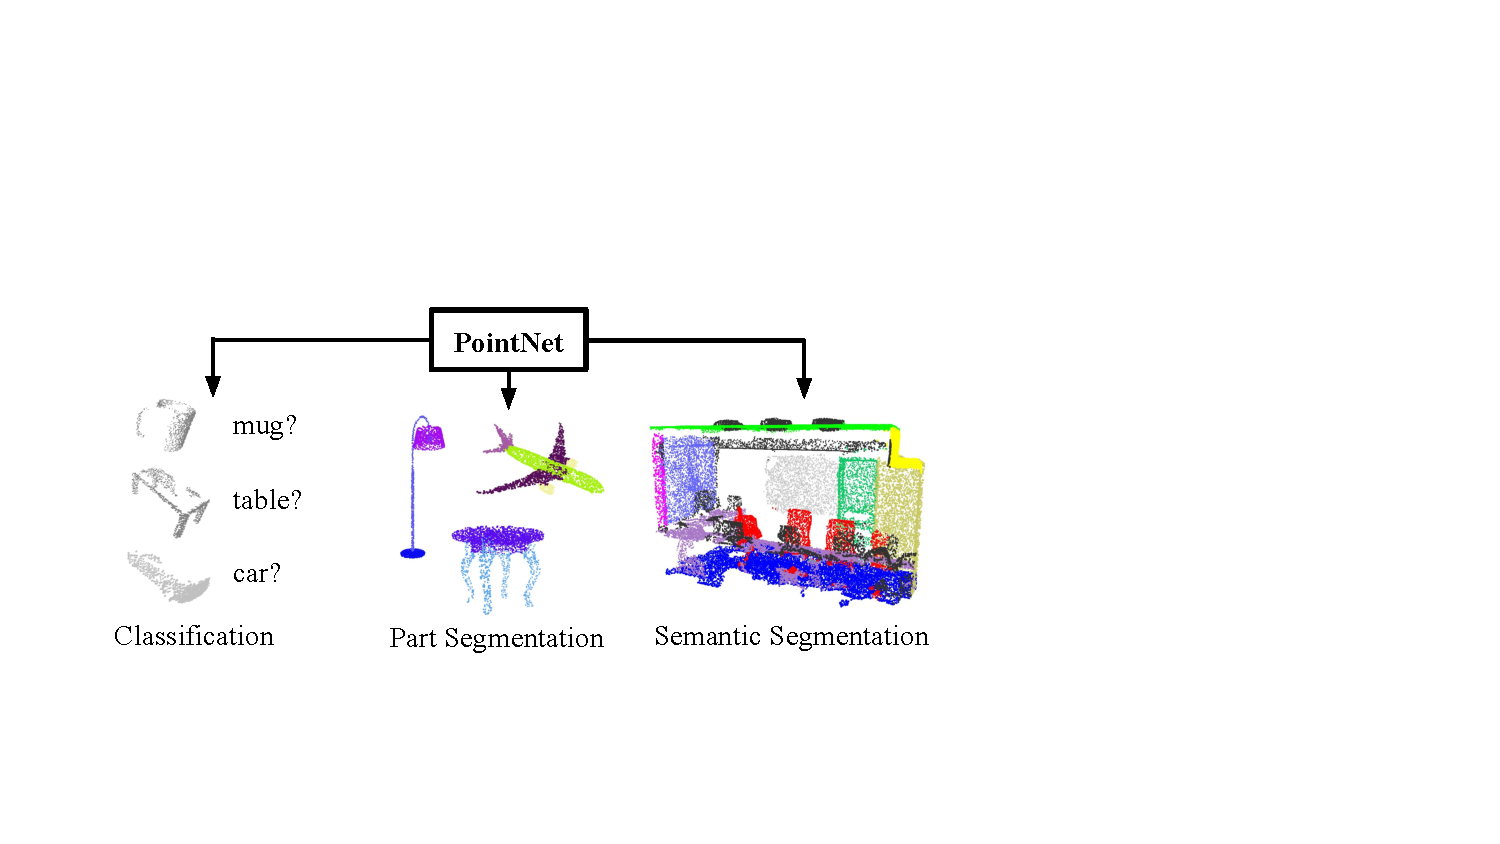
\includegraphics[width=\linewidth]{fig/teaser.pdf}
    \caption{\textbf{PointNet 的应用} 
    我们提出了一个新的神经网络结构,其输入为一个原始的点云(点的集合),没有经过体素化或预渲染。该网络具有一个统一的架构,能够学习全局和局部的点特征,从而为各种三维识别任务提供了一个简单、高速而有效的方法。 
    %We propose a novel deep net architecture that consumes raw point cloud (set of points) without voxelization or rendering. It is a unified architecture that learns both global and local point features, providing a simple, efficient and effective approach for a number of 3D recognition tasks.% 
    }
    \label{fig:teaser}
\end{figure}


\begin{figure*}[th!]
    \centering
    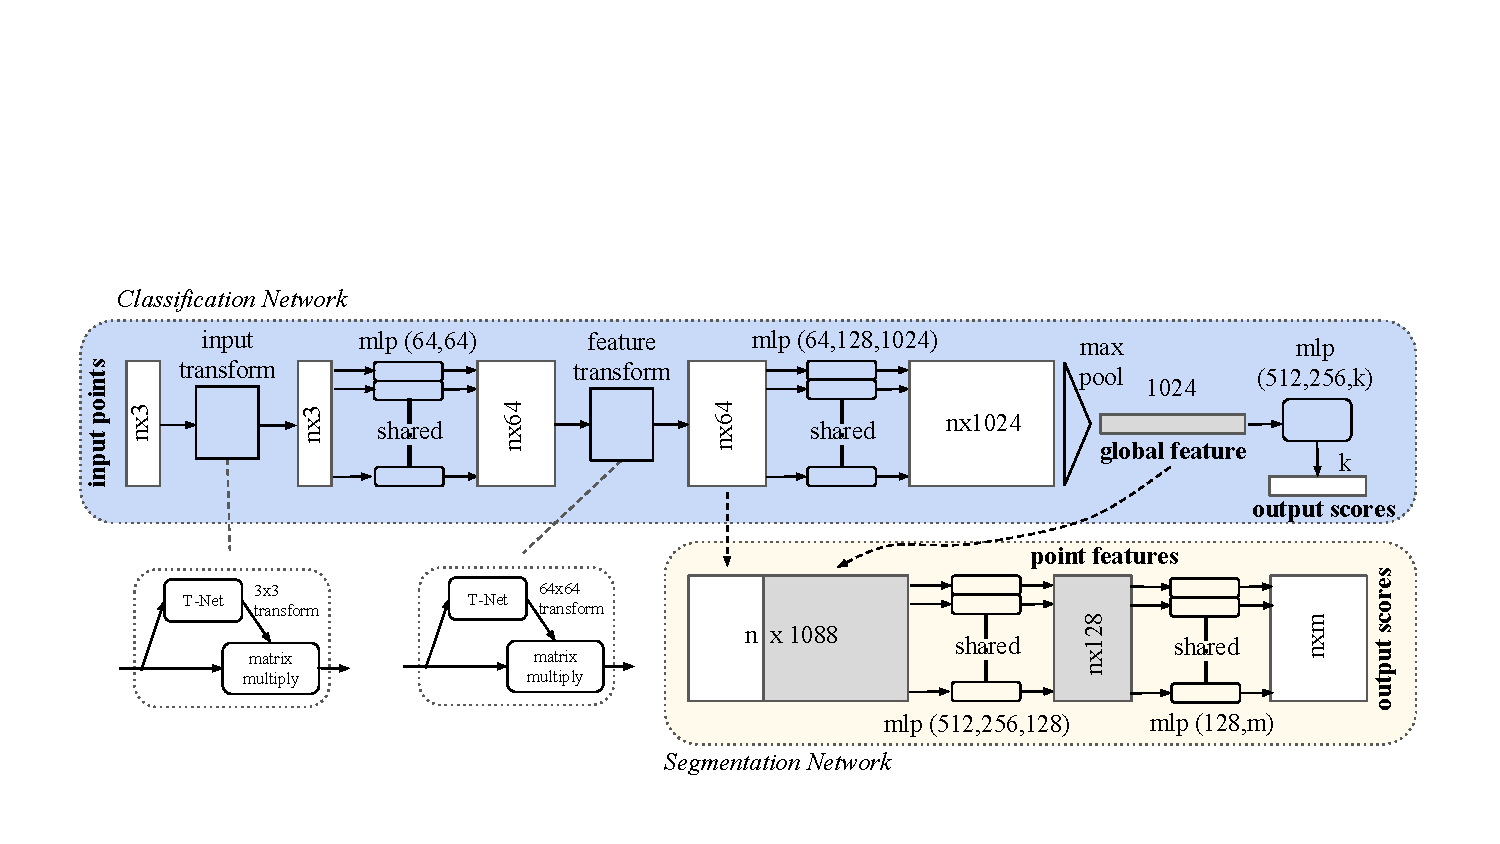
\includegraphics[width=0.9\linewidth]{fig/pointnet_fixed.pdf}
    \caption{\textbf{PointNet 架构}      分类网络将$n$个点作为输入,作用输入和特征变换,然后通过max pooling聚合点的特征,输出的是$k$种分类的分类分数。分割网络是分类网络的拓展,它连接局部和全局特征以及每个点输出的分数。``mlp''代表多层感知机,括号中的数字是层的大小。Batchnorm用于所有应用了ReLU的层。Dropout用于分类网络中的最后一个多层感知机。}
    \label{fig:pointnet_arch}
\end{figure*}

\section{相关工作}
\label{sec:related}
\begin{comment}
\todo{\\
  \paragraph{3d point cloud processing:}
  \begin{itemize}
    \item classification
    \item segmentation
    % \item correspondence
  \end{itemize} 
  traditionally, each 3d data processing task depends on some specific pipeline. our framework unifies them together.
  
  \paragraph{point cloud features:}
  \begin{itemize}
    \item global features
    \item local features
  \end{itemize}
  most works use hand-crafted features. 

  \paragraph{deep learning on 3d data:}
  \begin{itemize}
    \item multi-view CNN
    \item volumetric CNN
    \item spectral CNN on meshes 
    \item non end-to-end approach
  \end{itemize}
  in previous work of deep learning on point clouds, a point cloud is first converted to one of the above forms. however, there lacks work that directly operates on a raw point set.

  \paragraph{deep learning on unordered sets}
  \begin{itemize}
    \item discuss ``OrderMatters'', by Vinyals et al.
    \item say that this is a rather fundamental problem, related to many other tasks
  \end{itemize} 
}
\end{comment}

\paragraph{点云特征}
点云大部分的现有特征都是针对特定任务手工制作的。点特征通常编码某些统计特性,并且被设计成对于某些变换是不变的,这些变换通常被划分为内在的
\cite{aubry2011wave, sun2009concise, bronstein2010scale} 或外在的 ~\cite{rusu2008aligning, rusu2009fast, ling2007shape, johnson1999using, chen2003visual}。  它们还可以归类为局部特征和全局特征。对于特定任务,找到最优的特征组合并非易事。

%While one can extract all kinds of features and let a machine learning model decide which ones to use, the success of CNNs~\cite{lecun2015deep} for 2D images convinces us that an end-to-end feature learning paradigm is more promising. In this work we present a unified point feature learning network that can easily adapts to different tasks.

% \paragraph{Point Cloud Features}
% Most existing features for point cloud are handcrafted towards specific tasks. According to the spatial scopes, they can be categorized as local features and global features. Point features often encode certain statistical properties of points and are designed to be invariant to certain transformations, which are typically classified as being intrinsic [WKS, HKS] or extrinsic [PFH, FPFH, D2, spin image, LFD].

% Often one feature that works on task A may not perform well on task B. In addition, different features often make different assumptions of where the point cloud comes from. For example, HKS and WKS features work very well on organic objects such as human bodies, but they are not suitable for describing CAD models with combinatorial structures. For a specific task, it is not trivial to find the optimal feature combination for the task. 

% While one can extract all kinds of features and let a machine learning model to decide which ones to use, the success of CNNs [CITE] for 2D images convinces us that an end-to-end feature learning paradigm is more promising. In this work we present a unified point feature learning network that can easily adapts to different tasks, such as classification, segmentation, retrieval and correspondence. Our network directly works on point sets, due to its flexibility and broad usage in real applications.


\paragraph{3D数据的深度学习}
% \todo{we need to argue why point cloud (most close to raw sensor data), instead of meshes (not canonical), volume (sparsity), projected images (not in 3D, non-trivial to choose viewpoints) somewhere in the paper.}

3D数据具有多种流行的表示形式,从而有各种学习方法。
\emph{Volumetric CNNs:}~\cite{wu20153d, maturana2015voxnet, qi2016volumetric} 这是在体素形状上应用3D卷积神经网络的先驱。然而,由于数据的稀疏性和3D卷积的计算成本,体积表示受到其分辨率的限制。FPNN~\cite{li2016fpnn} 和 Vote3D~\cite{wang2015voting} 提出了处理稀疏性问题的特殊方法;然而,他们的操作仍然是在稀疏的体积上,处理非常大的点云对他们来说是一种挑战。
\emph{Multiview CNNs:}~\cite{su15mvcnn, qi2016volumetric} 试图将3D点云或形状渲染成2D图像,然后应用2D卷积神经网络对它们进行分类。通过精心设计的图像CNN,这一系列方法在形状分类和检索任务方面取得了突出的性能表现。~\cite{savvashrec}. 然而,将它们扩展到场景理解或其他3D任务例如点分类、形状完成上时表现很普通。
\emph{Spectral CNNs:} 最近的一些工作~\cite{bruna2013spectral, masci2015geodesic}在网格上使用了光谱CNN。但是这些方法目前受限于流形网格(例如有机物体),而且如何将它们扩展到非等距形状(例如家具)上并不明显。
\emph{Feature-based DNNs:}~\cite{fang20153d,guo20153d} 首先通过提取传统的形状特征将3D数据转换成向量,然后使用全连接网络对形状进行分类。我们认为它们受限于所提取特征的表示能力。

% In our work, we do deep learning directly on the raw 3D representation -- point clouds, without the pre-processing stage of converting them to volumes, images, graphs, or feature vectors. Therefore, our method has the potential to greatly simply the pipeline in practical usage.

% We argue that point cloud is a good representation in many aspects: 1) it's raw -- point clouds are the data acquired directly from depth sensors or laser scans, not like volumes or images that suffer from information loss. 2) it's in 3D, not like projected images that lack 3D geometry, which may require additional cross-view consistency mechanisms. 3) it's compact, not like volumetric grids that stores a 2D manifold surface in full 3D space. We design special networks to consume 3D point clouds and show that our network can be easily adapted for various 3D tasks with very good performance.


% Volumetric CNNs: [3DShapeNets, voxnet, our cvpr work] are the pioneers applying 3D convolutional neural networks on voxelized shapes. However, since sensors can only reach the surfaces of objects, most 3D data are just 2D manifold/surface living in a 3D space, thus volumetric grids are often sparse. Besides, the storage and computation cost both grow cubically with the input resolution. To address this challenge, [FPNN and vote3D] propose special methods to deal with the sparsity of volumetric representation; however, their operations are still performed on a very sparse volume and it is still challenging for them to process very large point clouds.

% Multiview CNNs: [MVCNN, our cvpr work, and some other image based methods] have tried to render 3D point cloud or shapes into 2D images and then apply 2D convolutional neural networks (using existing architectures such as AlexNet and VGG fine-tuned from ImageNet) to classify the shapes. With the well engineered image CNNs, this line of methods have achieved dominating performance on shape classification and retrieval tasks [cite SHREC]. However, it's nontrivial to extend them to scene understanding (not clear which camera positions to take), or other 3D tasks such as point classification and shape completion. Besides, when projecting 3D into images, we always have to convert predictions and data back and forth between 2D and 3D.

% Spectral CNNs: There has also been latest work that use spectral CNNs on meshes. However, these methods are currently constrained on manifold meshes such as organic objects and it's not obvious how to extend them to non-isometric shapes with sophisticated topological and geometric variations, such as furniture. Besides, acquiring meshes or point graphs require significant efforts in post processing from raw sensor data.

% Feature-based DNNs: [deep3dshape and Beihang's paper] firstly convert the 3D data into a vector, by extracting traditional shape features (HKS and WKS) and then use a fully connected neural network to classify the shape. We think they are constrained by the representation power of the features extracted.

% In our work, we do deep learning directly on the raw 3D representation -- point clouds, without the pre-processing stage of converting them to volumes, images, graphs, or feature vectors. Therefore, our method has the potential to greatly simply the pipeline in practical usage. We argue that point cloud is a good representation in many aspects: 1) it's raw -- point clouds are the data acquired directly from depth sensors or laser scans, not like volumes or images that suffer from information loss. 2) it's in 3D, not like projected images that lack 3D geometry, which may require additional cross-view consistency mechanisms. 3) it's compact, not like volumetric grids that stores a 2D manifold surface in full 3D space. We design special networks to consume 3D point clouds and show that our network can be easily adapted for various 3D tasks with very good performance.


\paragraph{无序集的深度学习}

从数据结构的角度来说,点云是无序的向量集合。当大部分深度学习工作集中在规则输入表示,如序列(语音和语言处理)、图像和体积(视频或3D数据)上时,很少有在点集上做深度学习工作的。

Oriol Vinyals等人最近的一项工作~\cite{vinyals2015order}研究了这个问题。他们使用具有注意机制的读取-处理-写入网络来处理无序输入集,同时展示他们的网络具有对数字进行排序的能力。然而,由于他们的工作重点是泛型集合和NLP应用,因此缺少了几何体在集合中的作用。

% Our work exploits the geometry properties in 3D point sets, provides theoretical analysis to what has been learned, gives rich visualizations to help understand the model. Our work also targets towards real applications of object classification and segmentation.

\section{问题陈述}
\label{sec:problem}
\begin{comment}
\todo{
  \begin{enumerate}
    \item we are interested in deep learning methods for object classification and segmentation on 3d point sets.
    \item we solve the two problems in a unified framework. in this framework, we use neural network to learn a function $f$ that takes a subset of points in $\R^3$ as input, and predicts the object recognition or per-point segmentation.  
  \end{enumerate}
}
\end{comment}

我们设计了一个能够将无序的点集作为输入的深度学习网络框架。一个点云可以由若干个三维点的集合表示 $\{P_i| \ i=1,...,n\}$,其中每个点 $P_i$ 都是其空间坐标 $(x,y,z)$ 和其他额外的特征频道(例如颜色、范数等)。出于简洁性和清晰性,除非特别指出,我们只使用三维空间坐标,即 $(x,y,z)$ 作为输入点的频道。

% We design a deep learning framework that directly consumes unordered point sets as inputs. %, while most recent state-of-the-art methods convert them to volumetric grids \cite{wu20153d,wang2015voting,qi2016volumetric} or projecting them to images \cite{su15mvcnn,qi2016volumetric}. % Furthermore, our proposed network is a unified framework for a various of applications including object classification, object-level part segmentation and scene semantic parsing. A point cloud is represented as a set of 3D points $\{P_i| \ i=1,...,n\}$, where each point $P_i$ is a vector of its $(x,y,z)$ coordinate plus extra feature channels such as color, normal etc. For simplicity and clarity, unless otherwise noted, we only use the $(x,y,z)$ coordinate as our point's channels. % Our network directly consumes the point cloud 

对于物品分类的任务,输入点可以直接采样自某一个形状,或是某个场景的点云预先分割好的结果。我们提出的深度网络为 $k$ 个候选分类输出 $k$ 个得分。对于语义分割任务,输入可以使一个用于零件部分分割的单个物体,也可以是一个 3D 场景下用于区域零件分隔的子空间。我们的模型将会为 $n$ 个点与 $m$ 个语义子分类输出  $n \times m$ 个得分。

% For the object classification task, the input point cloud is either directly sampled from a shape or pre-segmented from a scene point cloud. Our proposed deep network %first generate global descriptors for the whole input point cloud and then 
% outputs $k$ scores for all the $k$ candidate classes.
% For semantic segmentation, the input can be a single object for part region segmentation, or a sub-volume from a 3D scene for object region segmentation. Our model will output $n \times m$ scores for each of the $n$ points and each of the $m$ semantic sub-categories.



\section{点集上的深度学习}
我们提出的PointNet网络结构(\ref{sec:pointnet_arch}节)的灵感主要来源于\ref{sec:point_set_property}节所述的$\mathbb{R}^n$内点集的属性。 % We first describe the three properties in Sec~\ref{sec:point_set_property}; accordingly, we discuss our architecture designs in Sec~\ref{sec:pointnet_arch}, where we also summarize our whole network for classification and segmentation tasks. Furthermore, Sec~\ref{sec:theory} provides some theoretical analysis on how and why our network works well on point sets, though the architecture is not complicated.

\subsection{$\mathbb{R}^n$内点集的属性}
\label{sec:point_set_property}
网络的输入是来自欧几里得空间的点的子集,主要有一下三种主要的性质:

% \begin{itemize}
\bitem
\item 无序性。
不同于图片的像素或者立方体的体素,点云是一些无特定顺序的点的集合。换句话说,一个要处理$N$个3D点集的网络需要对按序输入的点集的$N!$种排序保持不变。 
\item 点之间有相互作用。这些点来自具有距离度量的空间。这意味着这些点不是孤立的,而且相邻的点形成一个具有意义的子集。因此,模型需要能够从邻近点中捕获局部结构,以及局部结构之间的组合相互作用。 
\item 转换的不变性。
作为一个几何体,已习得的点集表示需要对一些变换保持不变。例如,对一些点一起做旋转和平移变换既不会改变全局的点云类别、也不会改变点的分割。
\eitem
% \end{itemize}

% The above three properties of our input lead to the three key ideas of our network design, which are discussed respectively in the following section.


\subsection{PointNet的结构}
\label{sec:pointnet_arch}

我们的完整网络架构图如图\ref{fig:pointnet_arch}所示,其中用于分类的网络和用于分割的网络占据了网络结构中的很大一部分。请阅读图\ref{fig:pointnet_arch}的题注以了解流程。

我们的网络有三个关键模块:用作对称函数、聚类所有点的信息的最大池化层;一个局部和全局信息结合的结构;和两个对齐了输入点和点的特征的联合对齐网络。

我们将在以下的单独段落中讨论这些设计选择背后的原因。%, after a brief overview of the network.

% \paragraph{Overview} In basic PointNet: Given a point cloud input, for example, $n$ points of $(x,y,z)$ coordinates, the network firstly applies a function (multi-layer perceptron network) on each point independently. Function outputs across points are then aggregated with a max pooling layer. The aggregated vector is a global feature for the point cloud.
% 
% For classification task, the global feature is further passed through a few fully connected layers (with ReLU) to predict class scores for the entire point cloud.
% 
% For segmentation, we need to combine both local and global context for point class prediction. To this end, the global feature is appended to each point's local feature vector to provide a global context for individual point. We then apply a multi-layer perceptron net on the concatenated feature of each point to predict its class scores.
% 
% Additional input and feature space alignment network can be inserted, as shown in Fig~\ref{fig:pointnet_arch}. The alignment network is a regressor to transformation matrix and resembles the basic classification net in architecture.
% 

\paragraph{用于处理无序输入的对称函数}
为了使模型对输入排序不变,存在三种策略:1)将输入排列为规范顺序;2)将输入看作训练RNN的序列,但通过各种排列增加了训练数据;3)用一个简单的对称函数来聚类每个点的信息。这里,对称函数将$n$个向量作为输入,然后输出一个不受输入顺序变化影响的新向量。例如,$+$和$*$操作符是对称二元函数。 

尽管排序听起来像是一个简单的解决方法,但实际上谈及到一般意义上的点的扰动时,在高维空间中并不存在稳定的排序。这可以很容易地通过矛盾来显示。如果这样一种排序策略存在,那么它定义了高维空间和一维实线之间的双向映射。不难看出,谈及点扰动时要求排序的稳定等同在维度降低时保持映射在空间上的接近度,一般情况下这项任务是无法实现的。因此,排序并不能完全解决排序问题,而且因为排序问题的存在,网络很难学习到从输入到输出的一致映射。如实验(图\ref{fig:order_invariant})中所示,我们发现直接在排序点集上应用多层感知机的性能不好,尽管略优于直接处理无序输入。

使用RNN的方法是将点集作为顺序信号,并希望用随机排序的序列训练RNN,这样RNN将会变得和输入顺序无关。然而,在``OrderMatters''~\cite{vinyals2015order}中,作者已经证明顺序确实很重要而且无法完全被忽略。尽管RNN对于较短(几十个)的序列的输入排序已经具有相对良好的鲁棒性,但是很难扩展到像点集这样有成千上万的输入元素上。根据实验,我们也证明了基于RNN的模型在性能上不如我们所提出来的方法(图\ref{fig:order_invariant})。

我们的想法是通过对集合中转换元素应用对称函数来近似在点集上定义的一般函数:
\begin{align}
    f(\{x_1, \dots, x_n\})\approx g(h(x_1), \dots, h(x_n)),
    \label{eq:approx}
\end{align}
其中 $f:2^{\mathbb{R}^N} \rightarrow \mathbb{R}$, $h: \mathbb{R}^N\rightarrow \mathbb{R}^K$ 和 $g:\underbrace{\mathbb{R}^K\times \dots \times \mathbb{R}^K}_n \rightarrow \mathbb{R}$ 是对称函数。

根据实验,我们的基础模块十分简单:我们通过多层感知机来近似$h$,并通过单个变量函数和最大池化函数的组合来近似$g$。通过实验发现这样的模块结构表现的很好。通过$h$的集合,我们可以学到一些$f$来捕获点集的不同属性。 % This idea shares similar flavor with [cite leo's paper: probablistic shape fingerprint], where they define random functions on the input data and train a model based on the outputs of those optimization functions.  %Signature points are supposed to result in more extreme values for those random functions, thus the latter model can use weights to select them to make prediciton decisions for specific tasks. 
% In our architecture, instead of using random functions, we let the network itself learn a set of optimal functions to select signature points. 

尽管我们的关键模块看起来很简单,但它也具有很精彩的地方(参见\ref{sec:visualizing_pointnet}节),在一些不同的应用中能够表现出很强的性能(参见\ref{sec:application}节)。由于我们模块的简单性,我们也提供了\ref{sec:theory}节中的理论分析。


\paragraph{局部和全局信息聚类}
上一节的输出组成了一个向量$[f_1, \dots, f_K]$,这是输入集的全局标签。我们可以在形同全局特征上很容易训练SVM或多层感知机分类器以进行分类。然而,点的分割需要结合局部信息和全局信息。我们能够通过简单而高效的方式来实现这一目标。 % Even for global point classification, it could be beneficial to exploit more local geometries.

我们的解决方法可以在图\ref{fig:pointnet_arch}(\textit{Segmentation Network})中看到。在计算完全局点云特征向量后,我们将全局特征和每一个点的特征连接起来反馈给每一个点特征。然后我们基于组合的点特征提取新的每个点的特征,这样每个点特征都考虑了局部和全局信息。 % This structure can be repeated multiple times.

通过这样的修改,我们的网络能够预测依赖于局部几何和全局语义的每个点数量。例如我们可以准确地预测出每个点的法线(图中的补充),验证网络能够汇总来自该点的局部领域的信息。在实验环节中,我们也表明我们的模型可以在形状部分分割和场景分割方面实现最先进的性能。
    
\paragraph{联合对齐网络}
如果点云在经历了某些几何变换(比如刚性变换),那么点云的语义标签必须是不变的。因此我们希望已习得的点集表示不受这些变换影响。

一个自然的解决方法是在特征提取前将所有的输入集对齐到规范空间。Jaderberg等人~\cite{jaderberg2015spatial}介绍了一种通过采样和插值来对齐二维图像的空间变换的方法,通过在GPU上特别定制的层来实现。

与~\cite{jaderberg2015spatial}相比,我们的点云输入形式使我们能够以更简单的方式来实现这一目标。我们不需要发明任何新的层,也不需要像图像任务那样引入任何别名。我们通过一个小型网络(图~\ref{fig:pointnet_arch}中的T-net)预测仿射变换矩阵,并直接将该变换作用于输入点的坐标。这一小型网络本身类似于大型网络,由独立的点特征提取、最大池化和全连接层组成。更多关于T-net的细节将在附录中介绍。

这个想法可以进一步扩展到特征空间的对齐。我们可以在点的特征上插入另一个对齐网络,并预测特征变换矩阵以对齐来自不同输入点云的特征。然而,特征空间中的变换矩阵比空间变换矩阵的维度高很多,这极大地增加了优化的难度。因此,我们在softmax的训练损失中增加了一个正则化项。我们约束特征变换矩阵接近于正交矩阵:
\begin{equation}
    L_{reg} = \|I - AA^T\|_F^2,
\end{equation}
其中$A$是小型网络预测得到的特征对齐矩阵。正如我们所期待的,一个正交变换将不会损失任何输入的信息。我们发现通过增加正则化项,优化变得更加稳定,而且我们的模型实现了更好的性能。


\subsection{理论分析}
\label{sec:theory}
 
% \todo{
%   goal: show that this network is theoretically robust to perturbation and corruption (additional points and incompleteness) of input data.
%   \begin{itemize}
%     \item analyze the max pooling layer: it selects a finite set of key points. the cardinality of the key point set is constrained by the dimension of max pooling. 
%     \item add some understanding of the symmetry function, if we can
%   \end{itemize}
% }

\paragraph{通用近似性} 

我们首先展示我们的神经网络具备通用近似到连续的集合函数上的能力。由于集函数的连续性,直观上我们认为,一个输入点集上的微小扰动不应当引起函数值的剧烈变化,例如其分类任务或分割任务的表现分数。

%We first show the universal approximation ability of our neural network to continuous set functions. By the continuity of set functions, intuitively, a small perturbation to the input point set should not greatly change the function values, such as classification or segmentation scores.

形式化地, 令 $\mathcal{X}=\{S: S\subseteq [0,1]^m \text{ and } |S|=n\}$,   $f:\mathcal{X}\rightarrow \mathbb{R}$ 在 $\mathcal{X}$ 上关于赫斯多夫距离 $d_H(\cdot, \cdot)$ (即: $\forall \epsilon > 0, \exists \delta >0$, for any $S, S'\in\mathcal{X}$, if $d_H(S, S') < \delta$, 则有 $|f(S)-f(S')|< \epsilon$)的连续的集函数。 我们的理论认为在池化层给定足够多的神经元, $f$ 能被无限近似,即, 在 \eqref{eq:approx} 中的 $K$ 
已经足够大。

% Formally, let $\mathcal{X}=\{S: S\subseteq [0,1]^m \text{ and } |S|=n\}$,   $f:\mathcal{X}\rightarrow \mathbb{R}$ is a continuous set function on $\mathcal{X}$ w.r.t to Hausdorff distance $d_H(\cdot, \cdot)$, i.e., $\forall \epsilon > 0, \exists \delta >0$, for any $S, S'\in\mathcal{X}$, if $d_H(S, S') < \delta$, then $|f(S)-f(S')|< \epsilon$. Our theorem says that $f$ can be arbitrarily approximated by our network given enough neurons at the max pooling layer, i.e., $K$ in \eqref{eq:approx} is sufficiently large. 

\begin{theorem}

令 $f:\mathcal{X}\rightarrow \mathbb{R}$ 是一个关于赫斯多夫距离 $d_H(\cdot, \cdot)$ 的集函数。$\forall \epsilon > 0$, $\exists$ 一个连续函数 $h$ 和一个对称函数 $g(x_1, \dots, x_n)=\gamma \circ \mbox{MAX}$, 使得任意 $S\in\mathcal{X}$,

% Suppose $f:\mathcal{X}\rightarrow \mathbb{R}$ is a continuous set function w.r.t Hausdorff distance $d_H(\cdot, \cdot)$. $\forall \epsilon > 0$, $\exists$ a continuous function $h$ and a symmetric function $g(x_1, \dots, x_n)=\gamma \circ \mbox{MAX}$, such that for any $S\in\mathcal{X}$,


\begin{align*}
	\left|f(S) - \gamma\left(\underset{x_i\in S}{\mbox{MAX}}\left\{h(x_i)\right\}\right)\right| < \epsilon
\end{align*}

其中 $x_1, \ldots, x_n$ 是一系列在 $S$ 中任意顺序排列的元素,$\gamma$ 是一个连续函数, 且 $\mbox{MAX}$ 是一个取 $n$ 个向量最为输入,然后返回一个元素层面上的最大值的最大化向量运算符。

\end{theorem}

该定理的理论证明参见本文的附加材料。其主要思想是,在最差情况下,通过将空间划分成等体积的体素,网络的学习结果是到将点云转换为体积表示。而在实际情况下,网络会学习一个聪明得多的策略来探测空间,正如我们将在点函数的可视化中呈现的那样。

% The proof to this theorem can be found in our supplementary material. The key idea is that in the worst case the network can learn to convert a point cloud into a volumetric representation, by partitioning the space into equal-sized voxels. In practice, however, the network learns a much smarter strategy to probe the space, as we shall see in point function visualizations.

\begin{figure}[t!]
    \centering
    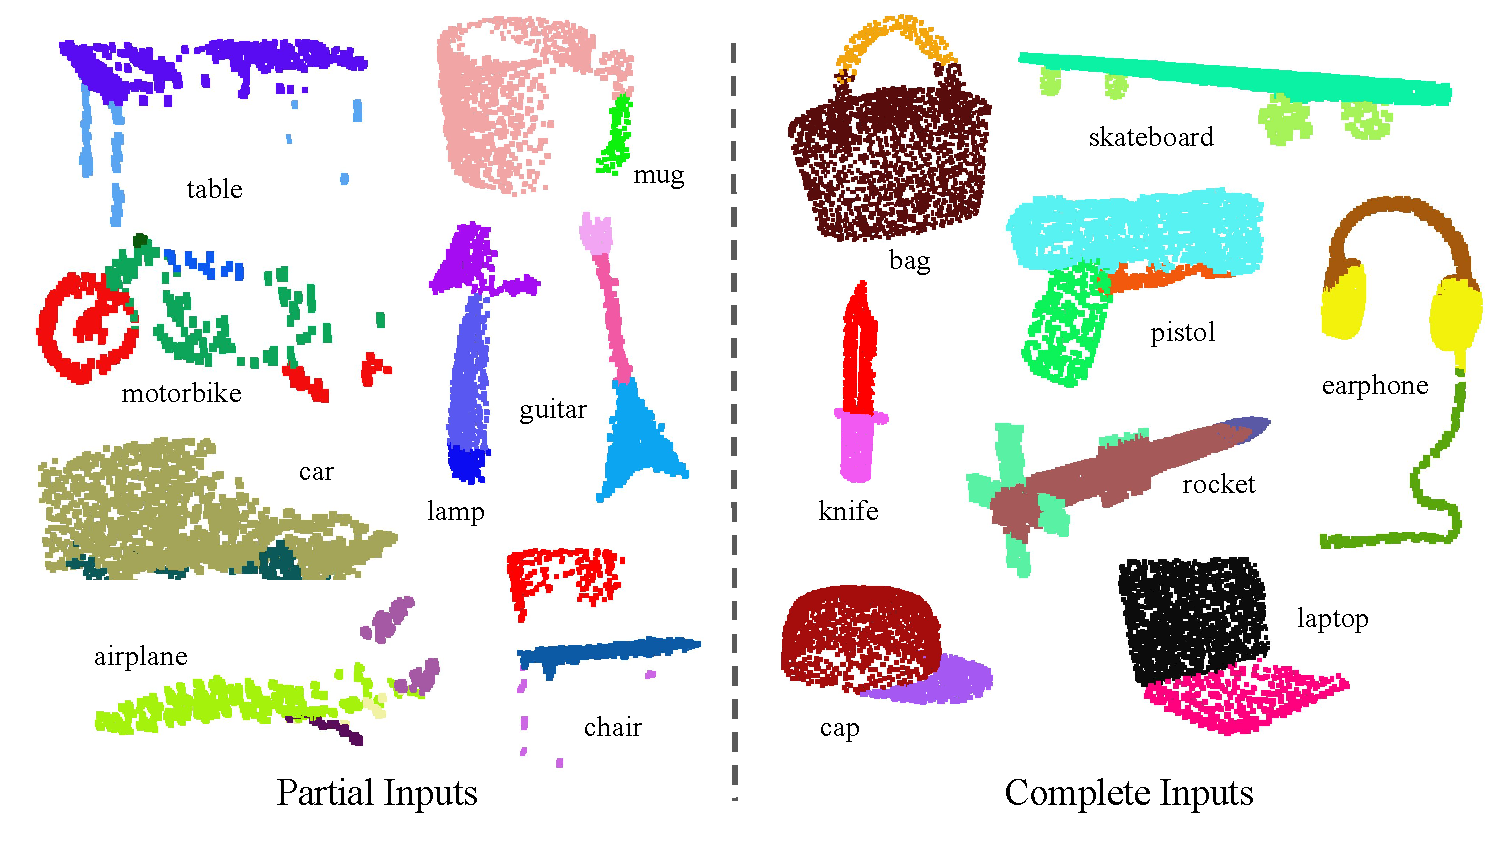
\includegraphics[width=0.8\linewidth]{fig/segres.pdf}
    \caption{
        \textbf{零件分割的量化结果} 我们可视化了横跨 16 个分类的 CAD 零件的分割结构。我们分别展示了部分模拟的 Kinect 扫描结果(左)和完全的 ShapeNet CAD 模型的结果(右)。
  %  \textbf{Qualitative results for part segmentation.} We visualize the CAD part segmentation results across all 16 object categories. We show both results for partial simulated Kinect scans (left block) and complete ShapeNet CAD models (right block).
    }
    \label{fig:qualitative_part_segmentation}
\end{figure}

\paragraph{瓶颈维度与稳定性} 从理论上和实践上,我们发现我们网络的表达性收到池化层维度的强烈影响。即,\eqref{eq:approx} 中的 $K$。在此我们提供了一个分析,同时也揭示了与我们模型的稳定性相关的一些属性。  

% \paragraph{Bottlenet dimension and stability} Theoretically and experimentally we find that the expressiveness of our network is strongly affected by the dimension of the max pooling layer, i.e., $K$ in \eqref{eq:approx}. Here we provide an analysis, which also reveals properties related to the stability of our model. 

我们定义 $\myvec u=\underset{x_i\in S}{\mbox{MAX}}\{h(x_i)\}$ 为网络 $f$ 的子网络。其中 $f$ 将分布在  $[0,1]^m$ 中的点集映射到了 $K$ 维空间的向量。接下来的理论分析指出,输入中的微小扰动或额外的噪音点不会严重影响我们网络的输出结果。

%We define $\myvec u=\underset{x_i\in S}{\mbox{MAX}}\{h(x_i)\}$ to be the sub-network of $f$ which maps a point set in $[0,1]^m$ to a $K$-dimensional vector. The following theorem tells us that small corruptions or extra noise points in the input set are not likely to change the output of our network:

\begin{theorem}

令 $\myvec u:\mathcal{X}\rightarrow \mathbb{R}^K$ 使得 $\myvec u=\underset{x_i\in S}{\mbox{MAX}}\{h(x_i)\}$ 且 $f=\gamma \circ \myvec u$. 则, 

% Suppose $\myvec u:\mathcal{X}\rightarrow \mathbb{R}^K$ such that $\myvec u=\underset{x_i\in S}{\mbox{MAX}}\{h(x_i)\}$ and $f=\gamma \circ \myvec u$. Then, 

\begin{enumerate}[label=(\alph*)]   

    \item $\forall S, \exists~\mathcal{C}_S, \mathcal{N}_S\subseteq \mathcal{X}$,  $f(T)=f(S)$ if  $\mathcal{C}_S\subseteq T\subseteq \mathcal{N}_S$;
    %\item Define the equivalence relation $\sim$ as $S\sim S'$ if $\myvec u(S)=\myvec u(S')$, then $\mathcal{C}_S=\underset{S'\sim S}{\cap} S'$ and $\mathcal{N}_S=\underset{S'\sim S}{\cup} S'$.
    % \item Let $S\sim S'$ if $\myvec u(S)=\myvec u(S')$. $\mathcal{C}_S=\underset{S'\sim S}{\cap} S'$, $\mathcal{N}_S=\underset{S'\sim S}{\cup} S'$.
    \item $|\mathcal{C}_S| \le K$
\end{enumerate}
\label{thm:thm2}
%     \begin{itemize}            
%     \item Critical points.
%     \\$\mathbb{C}=\{x_i: \myvec u_j(S)=h_j(x_i) \mbox{ for some } 1\le j\le K\}\cap S$
%     \item Free-space points.
%     \\$\mathbb{F}=\{x_i: \myvec u_j(S)<h_j(x_i) \mbox{ for some } 1\le j\le K\}\cap S$
%     \item Non-critical points. 
%     \\$\mathbb{N}=\{x_i: \myvec u_j(S)>h_j(x_i) \mbox{ for some } 1\le j\le K\}\cap S$
% For any $S'$ such that  $\mathbb{C} \subseteq S' \subseteq \mathbb{C}\cup\mathbb{N}$, $\myvec u(S')\equiv \myvec u(S)$; for any $S'$ such that $S'\cap \mathbb{F}\neq \emptyset$, $\myvec u(S')\neq \myvec u(S)$.
%\end{itemize}
\end{theorem}

关于上述定理,我们进一步阐释其推论。(a) 说明 $f(S)$ 在针对输入干扰时保持不变,只要  $\mathcal{C}_S$ 中的点被保留。同时也不会受到在 $\mathcal{N}_S$ 以内的额外噪声点的影响。(b) 说明 $\mathcal{C}_S$ 只包含一些有限数量的点,取决于 \eqref{eq:approx} 中的 $K$。换句话说,$f(S)$ 事实上是完全由一个元素数量小于或等于 $K$ 的有限子集 $\mathcal{C}_S\subseteq S$决定的。因此,我们将 $\mathcal{C}_S$ 称为 $S$ 的 \emph{关键点集},将 $K$ 成为 $f$ 的 \emph{瓶颈维度}。

% We explain the implications of the theorem. (a) says that $f(S)$ is unchanged up to the input corruption if all points in $\mathcal{C}_S$ are preserved; it is also unchanged with extra noise points up to $\mathcal{N}_S$. (b) says that $\mathcal{C}_S$ only contains a bounded number of points, determined by $K$ in \eqref{eq:approx}. In other words, $f(S)$ is in fact totally determined by a finite subset $\mathcal{C}_S\subseteq S$ of less or equal to $K$ elements. We therefore call $\mathcal{C}_S$ the \emph{critical point set} of $S$ and $K$ the \emph{bottleneck dimension} of $f$. 

结合 $h$ 的连续性,我们的模型关于点的扰动、缺失或额外的噪声点的健壮性得以解释。其健壮性的提升类似于机器学习模型中的稀疏原则。\textbf{直观上看,我们的模型能够通过一个稀疏的关键点来概括出形状。}在实验部分,我们可以看到从一个物体骨架的关键点。

% Combined with the continuity of $h$, this explains the robustness of our model w.r.t point perturbation, corruption and extra noise points. The robustness is gained in analogy to the sparsity principle in machine learning models. {\bf  Intuitively, our network learns to summarize a shape by a sparse set of key points.} In experiment section we see that the key points form the skeleton of an object.




\begin{comment}
\subsection{The properties of point sets in $\R^n$}
\todo{
  our input is a subset of points from a Euclidean space. It has three main properties:
  \begin{itemize}
    \item as a set, points in it has no order; 
    \item the points are from a metric space. therefore, local structures from near points have to be characterized;
    \item as a geometric object, the learned representation of the point set should be invariant to certain transformations.
  \end{itemize}
  the above three properties of our input leads to the three key ideas of our network design. we explain one by one.
}
\subsection{Unordered point set as input}
\todo{
  \begin{itemize}
    \item three strategies exist: 1) sorting input into a canonical order; 2)  use RNN but train order-invariantly; 3) use a symmetric function to aggregate the information from each point. 
    \item theoretically and empirically argue that the first two choices are not good. 
    \item our idea is to approximate a general function defined on a point set by applying a symmetric function on transformed elements in the set: $$f(\{x_1, \dots, x_n\})\approx g(h(x_1), \dots, h(x_n)),$$ where $f:2^{\R^N} \rightarrow \R$, $h: \R^N\rightarrow \R$ and $g:\R\times \dots \times \R\rightarrow \R$ is a symmetric function.
    \item we think this is provable for some good $f$.
    \item empirically, we approximate $h$ by a multi-layer perceptron network and $g$ by a composition of a single variable function and a max pooling function. this is found to work well by experiments.
    \item we can learn a number of $f$'s to capture different properties of the set.
  \end{itemize}
}

\subsection{Local and global information aggregation}
\todo{
  \begin{itemize}
    \item the output from the above section forms a vector $[f_1, \dots, f_M]$, which is a global signature of the input set.
    \item however, for tasks such as segmentation, we also need combine local information and global information. 
    \item xxx
  \end{itemize}
}

\subsection{Input and feature space alignment}
\todo{
  \begin{itemize}
    \item as we explained earlier, the learned representation of the point set should be invariant to certain transformations.
    \item we propose to apply an input dependent transformation for each instance to align all input set to a canonical space
    \item the input of our data are very friendly to geometric transformations, such as affine. we can therefore predict the transformation matrix by a neural network, named Joint Alignment Network.
    \item this idea can be extended to the alignment of feature space, as well
  \end{itemize} 
}

\subsection{PointNet architecture}
\todo{
  \begin{itemize}
    \item we implement the above ideas into a network for point set learning, named PointNet
    \item show the network for classification and explain 
    \item show the network for segmentation and explain
  \end{itemize}
}

\subsection{Theoretical Analysis}
\todo{
  goal: show that this network is theoretically robust to perturbation and corruption (additional points and incompleteness) of input data.
  \begin{itemize}
    \item analyze the max pooling layer: it selects a finite set of key points. the cardinality of the key point set is constrained by the dimension of max pooling. 
    \item add some understanding of the symmetry function, if we can
  \end{itemize}
}



\end{comment}

\section{实验}
\begin{table}[t!]
    \small
    \centering
    \begin{tabular}[width=\linewidth]{l|c|c|c|c}
    \hline
    ~               & input        & \#views    & accuracy & accuracy \\ 
    ~ & & & avg. class & overall \\ \hline
    SPH~\cite{kazhdan2003rotation}             & mesh        & - & 68.2         & -  \\ \hline
    3DShapeNets~\cite{wu20153d}     & volume       & 1        & 77.3  & 84.7 \\
    VoxNet~\cite{maturana2015voxnet}          & volume       & 12        & 83.0 & 85.9 \\
    Subvolume~\cite{qi2016volumetric}    & volume       & 20      & 86.0  & \textbf{89.2} \\ \hline
    LFD~\cite{wu20153d}             & image        & 10        & 75.5 & -\\
    MVCNN~\cite{su15mvcnn}           & image        & 80        & \textbf{90.1} & -\\ \hline
    Ours baseline  & point    & -     & 72.6  & 77.4\\
    Ours PointNet   & point   & 1        & 86.2 & \textbf{89.2} \\ \hline
    \end{tabular}
    \caption{\textbf{ModelNet40上的分类结果} 我们的网络在一系列3D输入的深度网络中达到最先进的效果。}
    \label{tab:classification}
\end{table}
\label{sec:exp}
实验被分成了四部分。首先,我们展示了PointNets可以应用于多个3D识别任务 (Sec~\ref{sec:application})。 其次,我们提供了详细的实验来验证我们的网络设计 (Sec~\ref{sec:arch_analysis})。最后,我们可视化了网络学到的内容 (Sec~\ref{sec:visualizing_pointnet}) 并且分析了时间和空间复杂度 (Sec~\ref{sec:complexity})。



\begin{table*}[th!]
    \small
    \centering
    \begin{tabular}[width=\linewidth]{l|c|p{0.5cm}p{0.4cm}p{0.4cm}p{0.4cm}p{0.5cm}p{0.6cm}p{0.5cm}p{0.5cm}p{0.5cm}p{0.6cm}p{0.6cm}p{0.3cm}p{0.5cm}p{0.6cm}p{0.6cm}p{0.6cm}}
    \hline
    ~        & mean & aero & bag & cap & car & chair & ear & guitar & knife & lamp & laptop & motor & mug & pistol & rocket & skate & table \\ 
    &   & &  &  &  &  & phone &  &   &  &  & &    &    &    & board &  \\ \hline
    \# shapes & & 2690 & 76 & 55 & 898 & 3758 & 69 & 787 & 392 & 1547 & 451 & 202 & 184 & 283 & 66 & 152 & 5271 \\ \hline
    Wu~\cite{Wu2014248} &  -  & 63.2  & - &      -    & -   & 73.5 & - &    - &    - &     74.4  & -    & - &   -   &   -   &   - & -  &  74.8 \\
    Yi~\cite{Yi16} & 81.4 & 81.0 & 78.4 & 77.7 & \textbf{75.7} & 87.6 & 61.9 & \textbf{92.0} & 85.4 & \textbf{82.5} & \textbf{95.7} & \textbf{70.6} & 91.9 & \textbf{85.9} & 53.1 & 69.8 & 75.3 \\ \hline
    3DCNN & 79.4 & 75.1 & 72.8 & 73.3 & 70.0 & 87.2 & 63.5 & 88.4 & 79.6 & 74.4 & 93.9 & 58.7 & 91.8 & 76.4 & 51.2 & 65.3 & 77.1 \\ 
    Ours & \textbf{83.7} & \textbf{83.4} & \textbf{78.7} & \textbf{82.5} & 74.9 & \textbf{89.6} & \textbf{73.0} & 91.5 & \textbf{85.9} & 80.8 & 95.3 & 65.2 & \textbf{93.0} & 81.2 & \textbf{57.9} & \textbf{72.8} & \textbf{80.6} \\ \hline
    \end{tabular}
    \caption{\textbf{ShapeNet数据集上的分割结果} 评价指标是点集的mIoU(\%)。 我们与两种传统方法 \cite{Wu2014248} \cite{Wu2014248} 以及我们提出的三维卷积网络对比。PointNet方法在mIoU上达到最佳表现。}
    %Notice that while all the other three methods are tested on the official ShapeNet train/validation/test split~\cite{shapenet2015}, the statistics for Wu's method~\cite{Wu2014248} are tested on a much larger set of shapes.
    \label{tab:segmentation}
\end{table*}



\subsection{应用}
\label{sec:application}
在本节中,我们将展示我们的网络是如何经过训练,来完成3D目标分类、目标零件分割和场景语义分割任务\footnote{更多应用样例,例如形状对应和基于点云的CAD模型检索包含在补充资料中。} 即使我们基于全新的数据表示(点集)进行研究,我们也能够在多个任务的基准测试中获得相当的甚至更好的性能。

\paragraph{3D目标分类} 我们的网络学习了可用于目标分类的全局点云特征。我们在ModelNet40~\cite{wu20153d} 形状分类基准上评估了我们的模型。总共有来自40个人造目标类别的12311个CAD模型,分为用于训练的9843个和用于测试的1468个。以前的方法主要集中于体积和多视图图像表示,我们提出了第一个直接处理原始点云的方法。

我们根据表面区域在网格面上均匀地采样了1024个点并将它们归一化为一个单位球体。在训练过程中,我们还通过沿上轴随机旋转对象并使用均值为0和标准差为0.02的高斯噪声抖动每个点的位置来动态地增强点云。


在表~\ref{tab:classification}中,我们将我们的模型与以前的相关工作,以及我们基于从点云中提取的传统特征(点密度、D2、形状轮廓等)MLP的基准线进行比较。我们的模型在基于3D输入(体积和点云)的所有方法中实现了最优的性能。仅仅使用全连接层和最大池化,我们的网络在推理速度上获得了强大的领先优势,并且也可以很容易地在CPU中并行化。但我们的方法与基于多视图的方法 (MVCNN~\cite{su15mvcnn}),之间仍然存在一点小差距,我们认为这是精细几何细节的丢失导致的,而这些细节可以被渲染图像所捕获。

\paragraph{3D目标零件分割} 零件分割是一项具有挑战性的细粒度3D识别任务。给定3D扫描或网格模型,任务是为每个点或面分配所属部分类别标签(例如椅子腿、杯柄)。
%The segmentation results are strong cues for part detection systems, which are key to many robotics applications such as grasping and affordance reasoning.

%Part segmentation requires knowledge of both local geometric and global semantics knowledge. By aggregating global feature vector to our point feature, our network is able to learn a \emph{deep point descriptor} that considers both local and global context, which suits well for this task.

我们对来自~\cite{Yi16}的ShapeNet部分数据集进行评估,其中包含来自16个类别的16881个形状,总共标注了50个部分。大多数目标类别都标有两到五个部分。对应的真实标签注释标记在形状上的采样点上。

我们将零件分割制定转换为每点分类问题。评估指标是点上的mIoU。对于类别C的每个形状S,计算形状的mIoU:对于类别C中的每个部分类型,计算真实和预测之间的IoU。如果真实点和预测点的并集为空,则将一部分IoU计为1。然后我们对类别C中所有部分类型的IoU进行平均以获得该形状的mIoU。为了计算类别的mIoU,我们取该类别中所有形状的mIoU的平均值。

在本节中,我们将我们的分割版PointNet (图~\ref{fig:pointnet_arch}的修改版, \textit{分割网络}) 和两种均利用了逐点几何特征和形状之间的对应关系的传统方法 \cite{Wu2014248} 和 \cite{Yi16} ,以及我们自有的3DCNN基准线进行了比较。有关3DCNN的详细修改和网络架构,请参阅补充说明。
%We design the segmentation 3D CNN architecture as a fully convolutional one that keeps volume size through all layers. In the end each voxel has a receptive field of 19 voxels with spatial resolution of 32.

在表~\ref{tab:segmentation}, 我们报告了每个类别和平均IoU(\%) 分数。我们观察到平均IoU有2.3\% 的提高,并且我们的网络在大多数类别中都优于基准方法。


\begin{table}[b!]
    \centering
    \small
    \begin{tabular}[width=\linewidth]{l|c|c}
    \hline
    ~             & mean IoU  & overall accuracy \\ \hline
    Ours baseline          &  20.12 & 53.19    \\ \hline
    Ours PointNet          & \textbf{47.71} & \textbf{78.62}  \\ \hline
    \end{tabular}
    \caption{\textbf{场景语义分割结果} 评价指标是13个类(结构和家具加上其他)的平均IoU和根据点集计算的分类准确率。 }
    \label{tab:semantic_segmentation}
\end{table}

\begin{table}[b!]
    \centering
    \small
    \begin{tabular}[width=\linewidth]{l|cccc|c}
    \hline
    ~                              & table & chair & sofa & board & mean  \\ \hline
    \# instance & 455 & 1363 & 55 & 137 & ~ \\ \hline
    Armeni et al.~\cite{armeni_cvpr16}          & 46.02 & 16.15 & \textbf{6.78} & 3.91  & 18.22 \\ \hline
    Ours & \textbf{46.67}     & \textbf{33.80 }    & 4.76    & \textbf{11.72}     & \textbf{24.24}     \\ \hline
    \end{tabular}
    \caption{\textbf{场景中3D物体检测结果} 评价指标是3D体积块中IoU阈值为0.5的平均准确率。}
    \label{tab:3d_detection}
\end{table}


% Move to supp
% While \cite{Wu2014248} and \cite{Yi16} deal with each object category independently, due to the lack of training data for some categories (the total number of shapes for all the categories in the data set are shown in the first line), we train our PointNet and the 3D volumetric CNN baseline across categories. To allow fair comparison, when testing these two models, we only predict part labels for the given specific object category. 

我们还对模拟Kinect扫描的任务进行了实验,来测试这些方法的稳健性。 对于ShapeNet部分数据集中的每个CAD模型,我们使用BlensorKinectSimulator~\cite{Gschwandtner11b} 从六个随机视点生成不完整的点云。我们根据这些完整形状和部分扫描数据,使用相同的网络架构和训练设置训练我们的PointNet。 结果表明,我们仅损失了5.3\%的平均IoU。 在图~\ref{fig:qualitative_part_segmentation}中,我们展示了针对完整数据和部分数据的定性结果。可以看到,虽然仅提供部分数据的任务相当具有挑战性,但我们的对其的预测是合理的。
%Since most real world scans are very partial due to occlusions, a model's robustness to partial input is key to evaluate its value in practice.


%From complete to partial input, we observed a $5.3\%$ mIoU drop. It is reasonable since lots of points are missed in virtual scans -- more structures need to be inferred. Still our model can segment well in some surprisingly partial cases, as shown in Fig~\ref{fig:qualitative_part_segmentation}, where both results on complete and partial data are displayed.

\begin{comment}
\begin{table}[h!]
    \small
    \centering
    \begin{tabular}[width=\linewidth]{l|cccc}
    \hline
    ~ & complete input & partial input \\ \hline
    3D CNN & 75.3 & 69.7 \\ \hline
    Ours PointNet & \textbf{80.6} & \textbf{75.3}  \\ \hline
    \end{tabular}
    \caption{\textbf{Segmentation results on partial scans.} Metric is mean IoU across all shapes.}
    %We perform rotation augmentation when training our PointNet on complete data to fairly compare with the simulated Kinect scans, that are generated from multiple perspective. In Table~\ref{tab:segmentation}, however, to compare with the traditional methods that rely on global orientation of shapes, no rotation augmentation is performed there.
    \label{tab:segmentation_partial}
\end{table}
\end{comment}

\paragraph{场景语义分割} 我们的零件分割网络可以很容易地扩展到语义场景分割,其中点标签成为语义目标类别,而不是目标的部分标签。
%Similar to image segmentation, we propose a 3D semantic segmentation task that organizes 3D points into semantic categories.

%Since our network operates on raw points, we can directly classify each point. On other hand, volumetric CNN and image based methods have to convert results back and forth in different representations.

% \begin{comment}
% Based on our net's ability to learn to classify 3D objects and segment point cloud, we can further achieve 3D object detection in scenes.
% \end{comment}

我们在斯坦福3D语义解析数据~\cite{armeni_cvpr16}上进行了实验。该数据集包含来自Matterport扫描仪的3D扫描结果,有6个大型室内区域组成,总共包括271个房间。扫描中的每个点都用来自13个类别(椅子、桌子、地板、墙壁等以及杂物)的语义标签中的一个进行注释。

为了准备训练数据,我们首先按房间分割点,然后将房间采样为面积为1mx1m的块。我们训练PointNet的分割版来预测每个块中的每个点类。每个点由XYZ、RGB和基于房间的归一化位置(从0到1)的9维向量表示。在训练时,我们实时的从每个块中随机采样4096个点。在测试时,我们对所有点进行测试。我们遵循与~\cite{armeni_cvpr16} 相同的协议,使用k-fold策略进行训练和测试。
%The sampled blocks have a overlap of half a meter. 


我们将我们的方法与使用人工设计点特征的基准线进行比较。基准线提取相同的9维局部特征和三个额外特征:局部点密度、局部曲率和法线。 我们使用标准MLP作为分类器。结果如表~\ref{tab:semantic_segmentation}所示,其中我们的PointNet方法明显优于基准线方法。 在图~\ref{fig:qualitative_segmentation}中,我们展示了定性分割结果。我们的网络能够输出平滑的预测,并且对缺失点和遮挡具有鲁棒性。




基于我们网络的语义分割输出,我们进一步构建了一个使用连接的组件进行目标采样的3D目标检测系统(有关详细信息,请参阅补充说明)。我们在表~\ref{tab:3d_detection}中与之前最先进的方法进行了比较。之前的方法基于滑动形状方法(带有CRF后处理),这种方法使用的支持向量机针对体素网格中的局部几何特征和全局房间上下文特征进行训练。我们的方法在所报告的家具类别上的效果大大优于它。

%we build a simple 3D object detection system. We use connected component with segmentation scores to get object proposals in scenes. For each proposed object, it's detection score is computed as the average point score for that category. Proposals with too less points or too small areas/volumes are pruned before evaluation. We observe that in some rooms such as auditoriums lots of objects (e.g. chairs) are close to each other, where connected component would fail to correctly segment out individual ones. Therefore we leverage our classification network and uses sliding shape method to alleviate the problem. The proposed boxes from connected component and sliding shapes are combined for final evaluation~\footnote{See supplementary for more details on implementation.}.



\begin{figure}[t!]
    \centering
    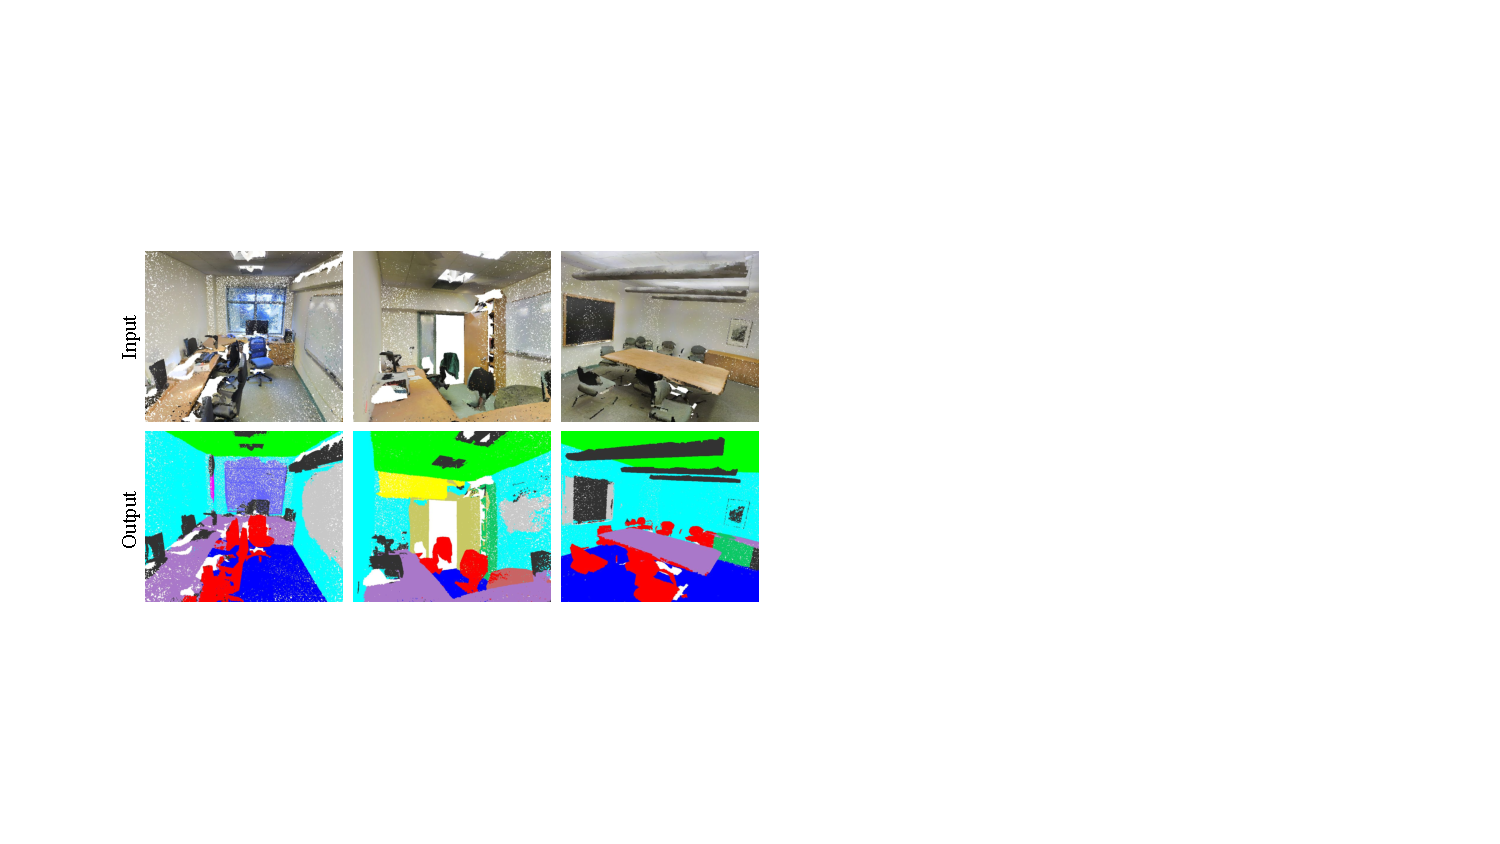
\includegraphics[width=0.8\linewidth,height=4cm]{fig/semantic}
    \caption{\textbf{语义分割的定性结果} 上一行是带颜色纹理的点云。底下是输出的语义分割结果(以点云展示),输出结果展示同输入的相机角度一致。}
    \label{fig:qualitative_segmentation}
\end{figure}

\subsection{架构设计分析}
\label{sec:arch_analysis}

在本节中,我们通过控制验证我们的设计选择实验。我们还展示了我们网络超参数的影响。
%~\footnote{Due to the limit of space, we refer the analysis on bottleneck dimension and number of input points to supplementary.}


\paragraph{与替代顺序不变方法的比较} 如第~\ref{sec:pointnet_arch}节所述,至少有三种选择可用于使用无序集合输入。我们使用ModelNet40形状分类问题作为测试平台来比较这些选项,以下两个控制实验也将使用此任务。

我们比较的基准线 (如图~\ref{fig:order_invariant}所示)包括:未排序和已排序的 $n \times 3$ 数组的多层感知机,将输入点视为序列的RNN模型,以及基于对称函数的模型。我们实验的对称操作包括最大池化、平均池化和基于注意力的加权和。注意方法类似于~\cite{vinyals2015order}中的方法,即从每个点特征预测一个标量分数,然后通过计算softmax跨点对分数进行归一化。然后根据归一化分数和点特征计算加权和。如图~\ref{fig:order_invariant}所示,最大池化操作以较大的优势幅度实现了最佳性能,这验证了我们的选择。


% \begin{table}
%     \small
%     \centering
%     \begin{tabular}[width=\linewidth]{l|c}
%     \hline
%     ~                    & accuracy \\ \hline
%     MLP (unsorted input) & 24.2       \\
%     MLP (sorted input)   & 45.0       \\
%     LSTM                 & 78.5       \\ \hline
%     Attention sum        & 83.0       \\
%     Average pooling      & 83.8       \\
%     Max pooling          & \textbf{87.1}       \\ \hline
%     \end{tabular}
%     \caption{\textbf{Comparing different order invariant methods.} Metric is classification overall accuracy on ModelNet40 test set. Max pooling is performing surprisingly well.}
%     \label{tab:order_invariant}
% \end{table}

\begin{figure}[t!]
    \centering
    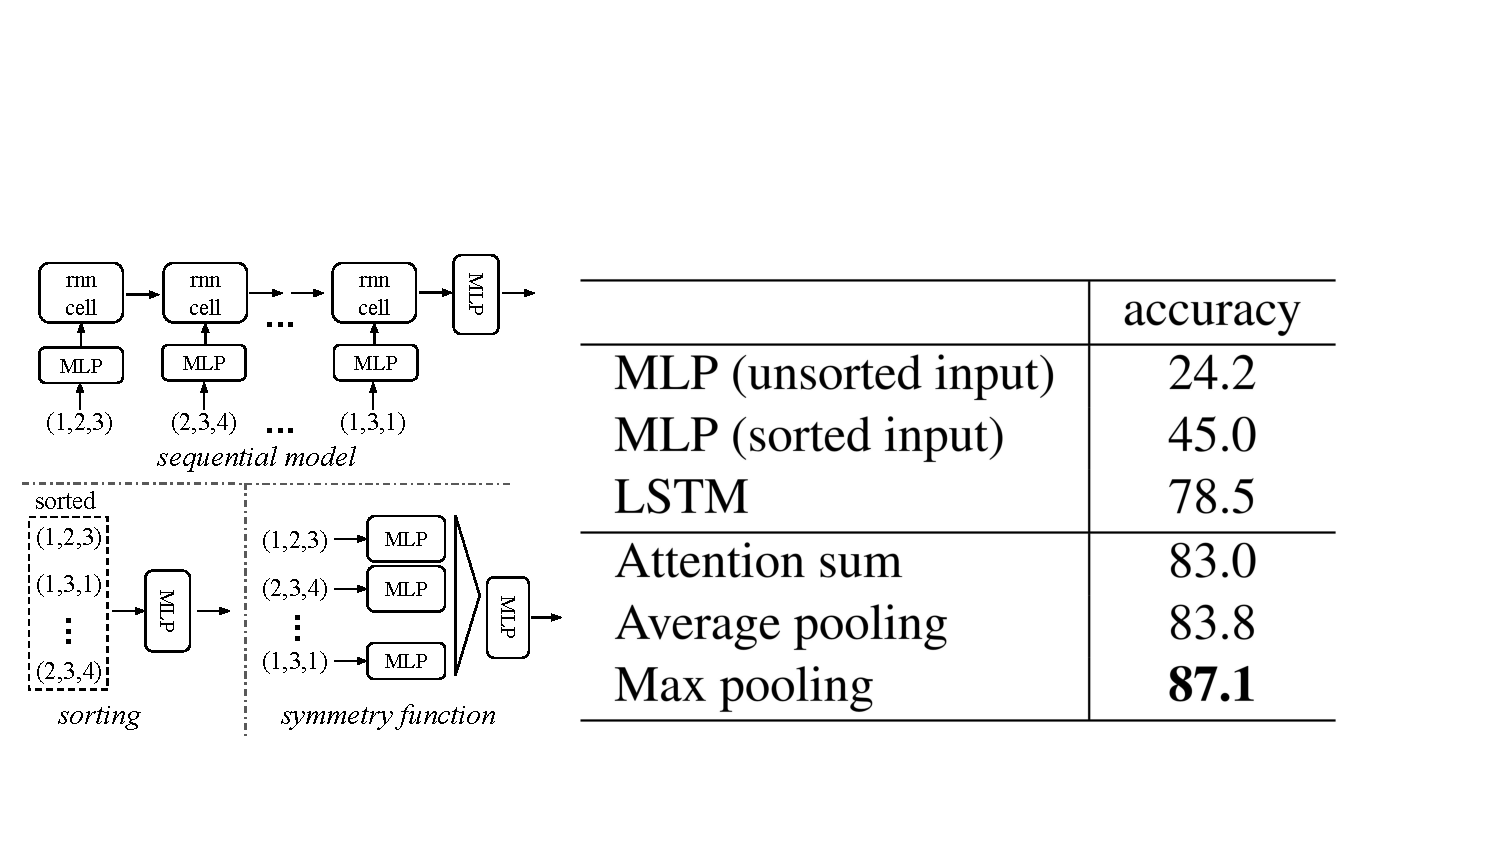
\includegraphics[width=\linewidth]{fig/order_invariant2.pdf}
    \caption{\textbf{三种实现顺序不变性的方法}神经元尺寸为64,64,64,128,1024,的5层隐藏层的多层感知机(MLP)应用在点集上,所有点共享一个简单的MLP副本。靠近输出的MLP共有两层,尺寸为512,256。}
    \label{fig:order_invariant}
\end{figure}

\paragraph{输入和特征转换的有效性} 在表~\ref{tab:transform}中,我们展示了我们的输入和特征转换(用于对齐)的积极影响。有趣的是,最基本的架构已经取得了相当合理的结果。使用输入转换可提高 $0.8\%$ 的性能。正则化损失是高维变换起作用所必需的。通过结合转换和正则化项,我们实现了最佳性能。

\begin{table}[b!]
    \small
    \centering
    \begin{tabular}[width=\linewidth]{l|c}
    \hline
    Transform              & accuracy \\ \hline
    none                   & 87.1     \\ \hline
    input (3x3)            & 87.9     \\
    feature (64x64)        & 86.9     \\
    feature (64x64) + reg. & 87.4     \\ \hline
    both                   & \textbf{89.2}     \\ \hline
    \end{tabular}
    \caption{\textbf{输入特征转换的效果} 评价指标是ModelNet40测试集上的总体分类准确率}
    \label{tab:transform}
\end{table}


% \paragraph{Effects of Max Layer Size and Number of Points} Here we show our model's performance change with regard to the size of the first max layer output as well as the number of input points. In Fig~\ref{fig:net_param} we see that performance grows as we increase the number of points however it saturates at around 1K points. The max layer size plays an important role, increasing the layer size from 64 to 1024 results in a $2-4\%$ performance gain. It indicates that we need enough point feature functions to cover the 3D space in order to discriminate different shapes.

% \begin{figure}
%     \centering
%     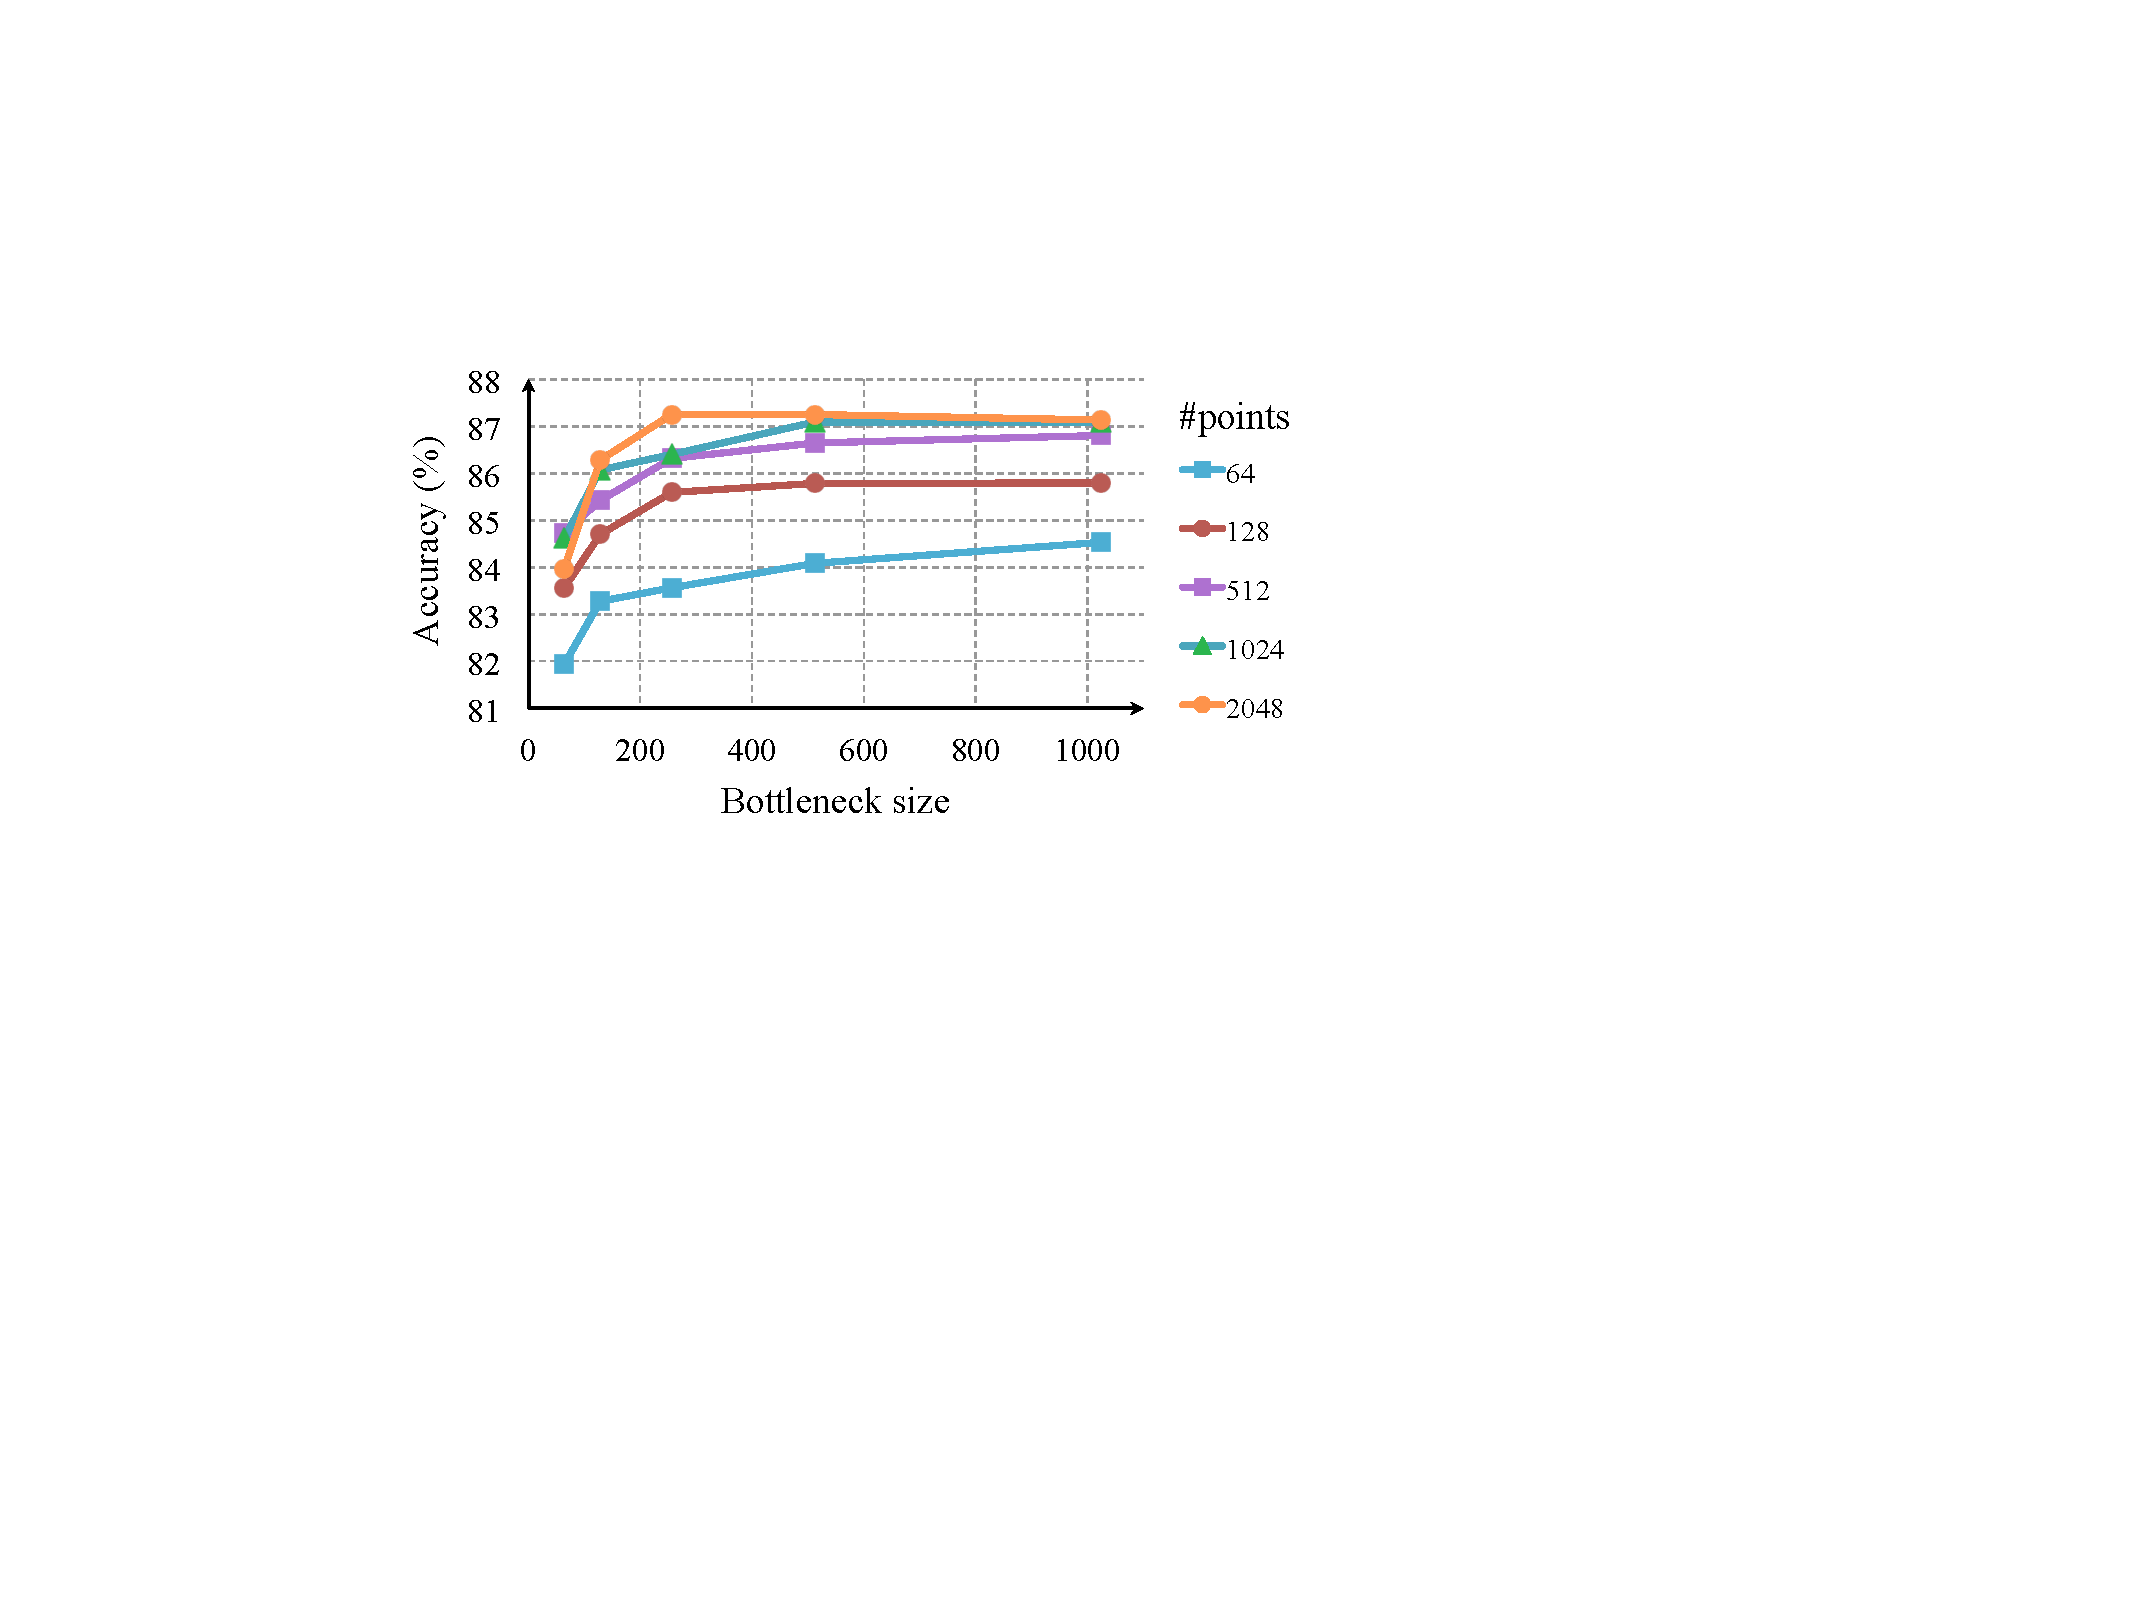
\includegraphics[width=0.8\linewidth]{fig/bottleneck.pdf}
%     \caption{\textbf{Effects of bottleneck size and number of input points.} The metric is overall classification accuracy on ModelNet40 test set.}
%     \label{fig:net_param}
% \end{figure}

\paragraph{鲁棒性测试} 我们展示了我们的PointNet不仅简单有效,还对各种输入损坏具有鲁棒性。我们使用与图~\ref{fig:order_invariant}的最大池化网络相同的架构。输入点被归一化为一个单位球体。结果如图~\ref{fig:robustness}。

A对于缺失点,当有 $50\%$ 的点缺失时,准确率仅下降 $2.4\%$ ,并且对于最远和随机输入采样则是 $3.8\%$ 。我们的网络在训练期间看到了异常点你,那么它对异常点也具有鲁棒性,。我们评估了两种模型:一种在具有 $(x,y,z)$ 坐标的点上进行训练;另一个在 $(x,y,z)$ 上加上点密度。即使当 $20\%$ 的点是异常值,网络也有超过 $80\%$ 的准确率。图~\ref{fig:robustness}右侧显示了网络对点扰动的鲁棒性。

\begin{figure}
    \centering
    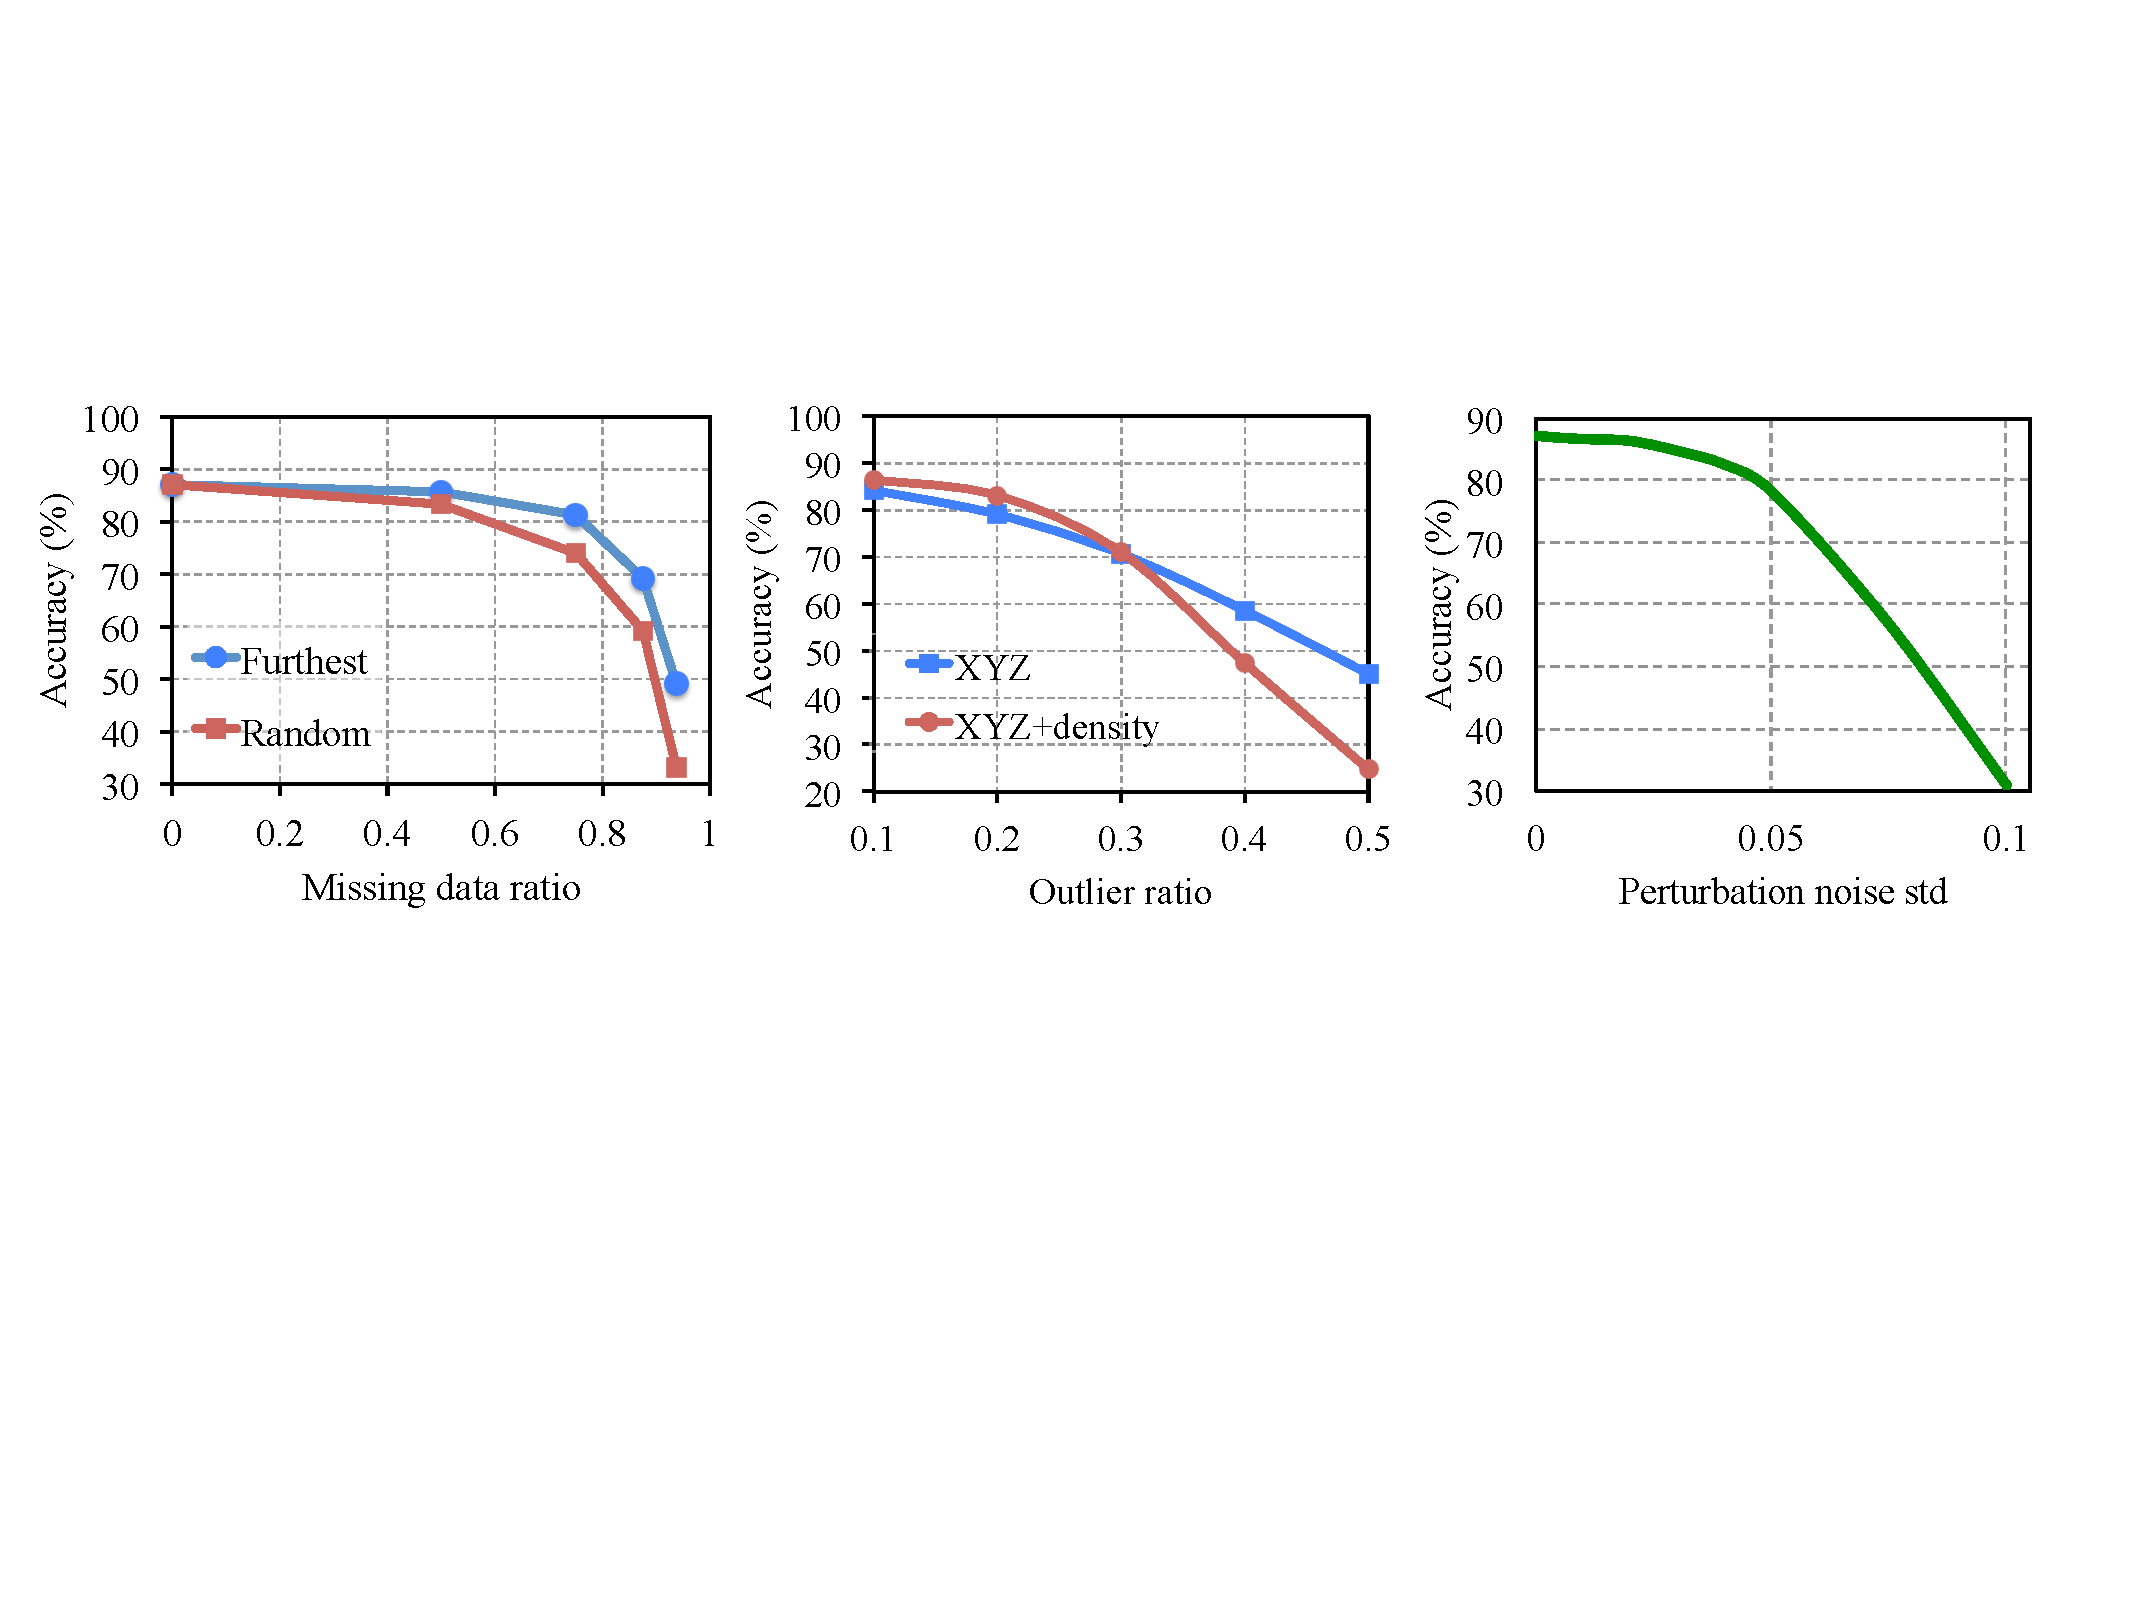
\includegraphics[width=\linewidth]{fig/robustness.pdf}
    \caption{\textbf{PointNet鲁棒性测试} 评价指标是ModelNet40测试集上的总体分类准确率。 左侧: 删除点的情况 Furthest意思是对1024个原始点采用最远点采样。 中间: 离群点插入的情况。离群点均匀的分布在单位球体中。 右侧: 点扰动的情况。单独对每个点进行高斯噪声扰动}
    \label{fig:robustness}
\end{figure}

\begin{comment}
\paragraph{MNIST Digit Classification} While we focus on 3D point cloud learning, a sanity check experiment is to apply our network on a 2D point clouds - pixel sets.

To convert an MNIST image into a 2D point set we threshold pixel values and add the pixel (represented as a point with XY coordinate in the image) with values larger than 128 to the set. We use a set size of 256. If there are more than 256 pixels int he set, we randomly subsample it; if there are less, we pad the set with the one of the pixels in the set (due to our max operation, which point used for the padding will not affect outcome). 
3
As seen in Table~\ref{tab:mnist}, we compare with a few baselines including multi-layer perceptron that considers input image as an ordered vector, a RNN that consider input as sequence from pixel (0,0) to pixel (27,27), and a vanila CNN. It's interesting to see that our model can achieve quite good performance by considering the image as a 2D point set.

% vanila CNN: https://www.microsoft.com/en-us/research/publication/best-practices-for-convolutional-neural-networks-applied-to-visual-document-analysis/
\begin{table}[h!]
    \centering
    \begin{tabular}[width=\linewidth]{l|c|c}
    \hline
    ~                      & input & error (\%) \\ \hline
    Multi-layer perceptron~\cite{simard2003best} & vector & 1.60  \\
    LeNet5~\cite{lecun1998gradient}                 & image & 0.80 \\ \hline
    Ours PointNet          & point set & 0.78 \\ \hline
    \end{tabular}
    \caption{\textbf{MNIST classification results.} We compare with vanila versions of other deep architectures to show that our network based on point sets input is achieving reasonable performance on this traditional task.}
    \label{tab:mnist}
\end{table}
\end{comment}


% \begin{figure}[b!]
%     \centering
%     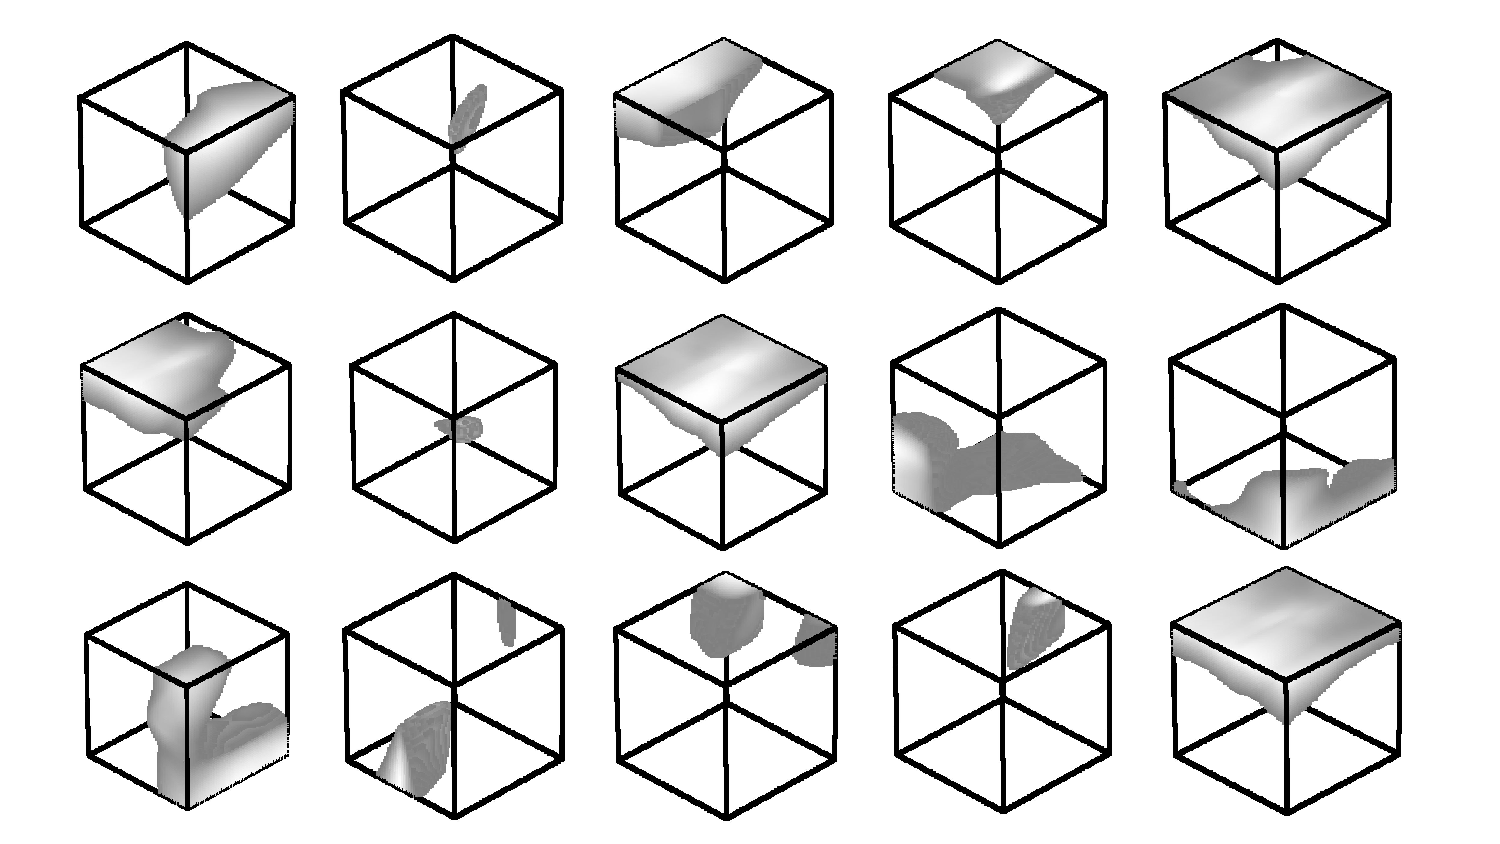
\includegraphics[width=0.7\linewidth]{fig/kernels.pdf}
%     \caption{\textbf{Point function visualization.} For each per-point function $h$, we calculate the values $h(p)$ for all the points $p$ in a cube of diameter two located at the origin, which spatially covers the unit sphere to which our input shapes are normalized when training our PointNet. In this figure, we visualize all the points $p$ that give $h(p)>0.5$ with function values color-coded by the brightness of the voxel. We randomly pick 15 point functions and visualize the activation regions for them.}
%     \label{fig:functions}
% \end{figure}


\subsection{可视化PointNet}
\label{sec:visualizing_pointnet}
% We design two experiments to visualize what has been learnt by the PointNet. The results are consistent with the theoretical analysis in Sec~\ref{sec:theory}. In the first experiment, we visualize the learnt point function $h(x)$ in Eq~\ref{eq:approx}, which demonstrates that our network learns a family of optimization criteria that selects informative points from the cloud. Our second experiment illustrates the robustness of our network, as explained in Thm~\ref{thm:thm2}.

% \paragraph{Point Function Visualization} As discussed in Sec~\ref{sec:pointnet_arch}, our network computes $K$ (we take $K=1024$ in this experiment) dimension point features for each point and aggregates all the per-point local features via a max pooling layer into a single $K$-dim vector, which forms the global shape descriptor. 

% To gain more insights on what the learnt per-point functions $h$'s detect, we visualize the points $p_i$'s that give high per-point function value $f(p_i)$ in Fig~\ref{fig:functions}. This visualization clearly shows that different point functions learn to detect for points in different regions with various shapes scattered in the whole space. 

\begin{comment}
This visualization is similar to the kernel visualization in convolutional neural networks in the sense that we'd like to know what input patterns would activate a specific neuron. However, our point function is behaving in a very differnt way from conv kernels.
\end{comment}

在图~\ref{fig:recon},我们可视化了一些样本形状 $S$ 的 \textit{关键点集} $\mathcal{C}_S$ 和 \textit{上边界形状} $\mathcal{N}_S$ (如Thm~\ref{thm:thm2}所述)。两个形状之间的点集将给出完全相同的全局形状特征 $f(S)$。

从图~\ref{fig:recon} 可以清楚地看出, \textit{关键点集} $\mathcal{C}_S$中对最大池化特征有贡献的点,总结了形状的主干。
%, or sample a sparse collection of points to describe the geometry of the whole shape.
\textit{上界形状} $\mathcal{N}_S$ 说明了与输入点云 $S$ 具有相同全局形状特征 $f(S)$ 的最大可能点云。$\mathcal{C}_S$ 和 $\mathcal{N}_S$反映了PointNet的鲁棒性,这意味着丢失一些非关键点不会改变全局形状特征 $f(S)$。



% We visualize the shape family, as discussed in Thm~\ref{thm:thm2}, including all the shapes between the \textit{critical point set} $\mathcal{C}_S$ and the \textit{upper-bound shape} $\mathcal{N}_S$ that gives the same global feature $f(S)$ with respect to a given shape $S$.

\begin{figure}[b]
    \centering
    % \includegraphics[width=0.8\linewidth]{fig/recon.pdf}
    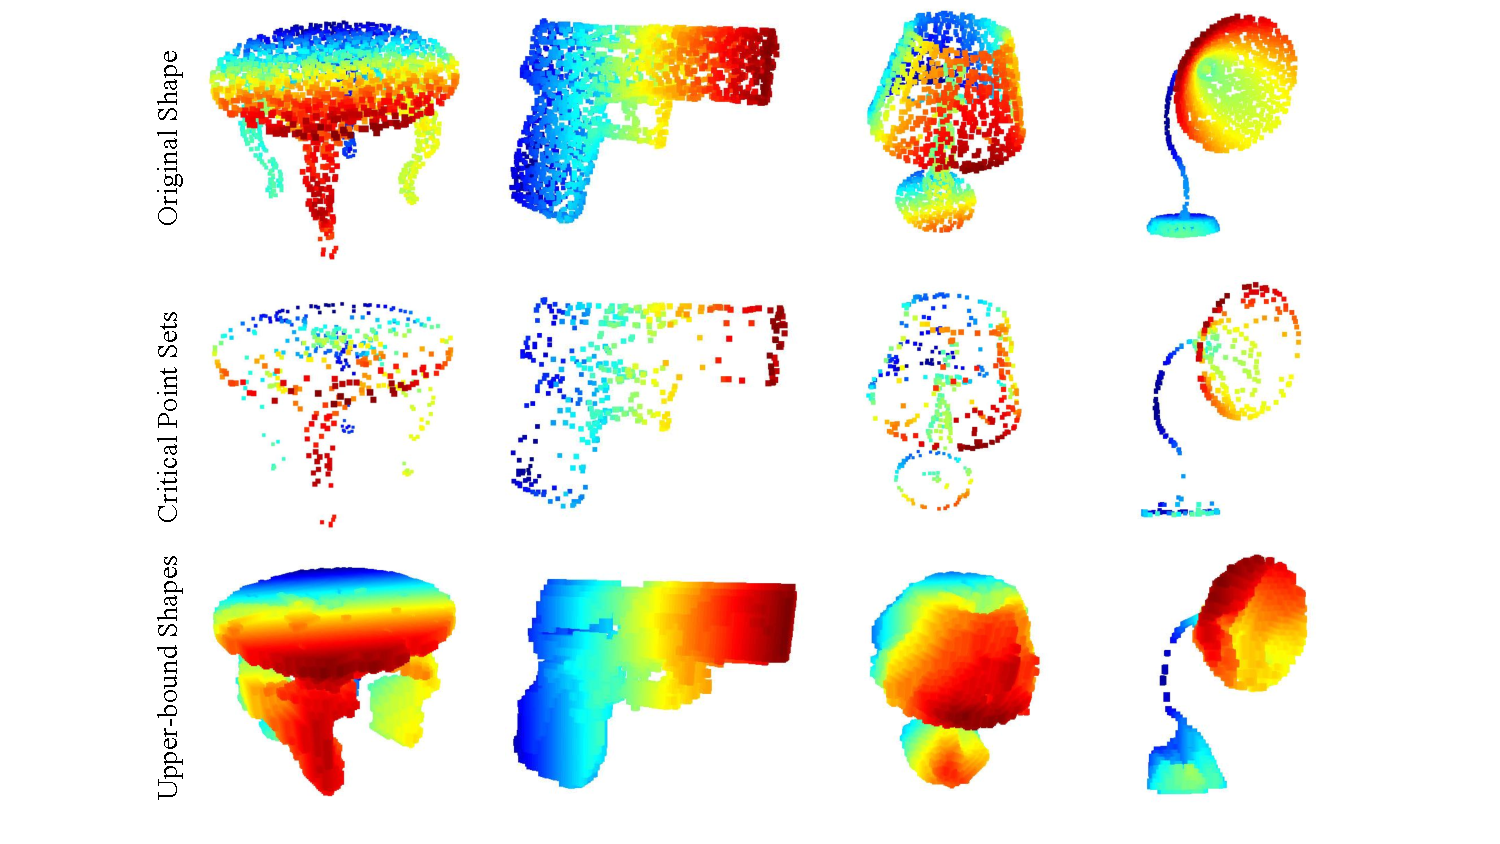
\includegraphics[width=0.8\linewidth]{fig/kp_ss_visu1.pdf}
    \caption{\textbf{关键点集和上界形状} 关键点集和上界形状共同决定了给定形状的全局形状特征,任何处于关键点集和上界形状间的点云都有同样一致的特征。 我们通过色彩编码来体现物体的深度信息。}
    \label{fig:recon}
\end{figure}

% Fig~\ref{fig:recon} shows the \textit{critical point sets} $\mathcal{C}_S$ and \textit{upper-bound shapes} $\mathcal{N}_S$ for four selected shapes. 
%The original input point clouds are rendered in the first row while the $\mathcal{C}_S$ and $\mathcal{N}_S$ for them are shown in the second and their rows respectively.
%The $\mathcal{C}_S$ for a given shape $S$ includes the points from the original point cloud that activates some point function $h_i$'s the most. 
$\mathcal{N}_S$ 是通过将边长为2的立方体中的所有点经过网络前向传播后,选择点函数值$(h_1(p), h_2(p), \cdots, h_K(p))$ 不大于全局形状描述符的点 $p$ 来构建的。
% It is not hard to see that all the shapes $S'$ that cover $\mathcal{C}_S$ and are contained by $\mathcal{N}_S$ give the exactly same global feature $f(S')=f(S)$. The transition shape family entails the robustness of the our PointNet, meaning that adding noisy jitterings or losing some non-critical points do not change the learnt shape signature and thus do not affect our classification or segmentation results.

\begin{comment}
We start from a max pooled vector of a specific input point cloud $X$, and find a set of point cloud $S$ (it's a set of point sets) where each point cloud in the set $S$ will result in the same max pooled vector as to $X$. In another word, we will reconstruct the input with only the knowledge of $X$ and the network parameters.

Assuming when feeding input point cloud $X$ to the network the first max-pooling layer's output is $g(X) = MAX\{f(x_1), f(x_2), ..., f(x_N)\} \in \R^{1024}$, where $X = \{x_1, x_2, ..., x_N\}$. We achieve the reconstruction by firstly construct a dense volumetric grids. Each voxel represents a point in 3D space. Then we will sweep through each point $p$ in the volume and judge whether this point's feature $f(p) \in \R^{1024}$ has any value larger than that in the corresponding dimension of $g(X)$. If there is , it means the point $p$ cannot be the input that results in $g(X)$, so we will exclude this point. After sweeping the volume, all the points left are possible to be part of the input set $X$. This set of points forms a upper bound of any possible input set that gets max pooling outcome of $g(X)$. Some reconstructed results of this upper bound is visualized in the second row of Fig~\ref{fig:recon}.

On the other hand, if we know the input set (set $X$) and the network, we can know which input points (subset $Y$ of $X$) are actually contributing to the final value of the max pooled vector. Excluding all the points in $X \\ Y$ will not affect the result. We call this contributing set of points the lower bound of the input, as visualized in the third row of Fig~\ref{fig:recon}. Any point sets that fall between the lower bound and upper bound will result in exactly the same result.
\end{comment}





\subsection{时间和空间复杂度分析}
\label{sec:complexity}
表~\ref{pointnet_complexity} 总结了我们PointNet分类网络的空间(网络中的参数个数)和时间(浮点运算/样本)复杂性。我们还将PointNet与之前工作中的一组具有代表性的基于体积和多视图的架构进行了比较。

尽管MVCNN~\cite{su15mvcnn} 和Subvolume (3D CNN) ~\cite{qi2016volumetric} 实现了高性能,PointNet的计算成本更低,效率更高(以FLOPs/样本衡量:效率分别提高\emph{141倍} 和 \emph{8倍})。此外,就网络中的\#param(参数少\emph{17倍})而言,PointNet的空间效率比MVCNN高得多。此外,PointNet更具可扩展性——它的空间和时间复杂度为 $O(N)$ —— 与输入点的数量呈\emph{线性} 关系。然而,由于卷积占用计算时间,多视图方法的时间复杂度随图像分辨率\emph{平方级}增长,基于体积卷积的方法随着体积大小成\emph{立方级}增长。

根据经验,PointNet能够处理超过每秒100万个点用于点云分类(约1K对象/秒)或语义分割(约2个房间/秒),在TensorFlow上使用1080XGPU,显示出实时应用的巨大潜力。

\begin{table}[h!]
    \centering
    \begin{tabular}{|l|l|l|l|}
    \hline
    ~                & \#params & FLOPs/sample\\ \hline
    PointNet (vanilla)  & 0.8M                        & 148M \\
    PointNet         & 3.5M                         & 440M \\ \hline
    %VoxNet~\cite{maturana2015voxnet}           & 0.07M                        & 204M \\
    Subvolume~\cite{qi2016volumetric} & 16.6M                        & 3633M \\ \hline
    MVCNN~\cite{su15mvcnn}   & 60.0M                          & 62057M \\ \hline
    \end{tabular}
    \caption{\textbf{处理3D数据分类的深度学习架构的时间和空间复杂度} PointNet (vanilla) 是分类版的PointNet除去输入和特征转化部分的版本。 FLOP代表浮点运算操作。
    ``M'' 代表百万。 Subvolume和MVCNN都使用了多次旋转和多个视角池化后的数据,没有这些操作他们的表现会大大下降}
    \label{pointnet_complexity}
    \vspace{-3mm}
\end{table}

\section{结论}
\label{sec:conclusion}
在这项工作中,我们提出了一种新颖的、可以直接使用点云输入的深度神经网络 \emph{PointNet} 。我们的网络为许多3D识别任务提供了统一的方法,这些3D识别任务包括目标分类、零件分割和语义分割,同时在标准基准上获得与现有技术相当或更好的结果。我们还提供理论分析和可视化来理解我们的网络。



\mypara{致谢} 作者非常感谢三星GRO授予的资助、ONR MURI N00014-13-1-0341的资助、NSF授予资助IIS-1528025、Google重点研究奖、来自Adobe公司的礼物和NVIDIA的硬件捐赠的支持。

{\small

\begin{thebibliography}{}
\documentclass[10pt,twocolumn,letterpaper,UTF8]{article}
\hyphenpenalty=2000
\textwidth=6.5in
\textheight=9.0in
\evensidemargin=0.0in
\oddsidemargin=0.0in
\topmargin=-0.5in
\clubpenalty=4000
\widowpenalty=4000
\displaywidowpenalty=500

\newlength\minalignvsep

\usepackage{cvpr}
\usepackage{times}
\usepackage{epsfig}
\usepackage{graphicx}
\usepackage{amsmath,amssymb,amsthm}
\usepackage{pbox}
\usepackage{epstopdf}
\usepackage{subfigure}
\usepackage{xspace}
\usepackage{comment}
\usepackage{lipsum}
%\usepackage{jeffe}
\usepackage{enumitem}

% 中文支持
\usepackage{ctex}
\usepackage[T1]{fontenc}
\usepackage{mathpazo}
\usepackage{fontspec}
\setmainfont[Scale = 1]{TeX Gyre Pagella}
\setCJKmainfont[ItalicFont=Noto Serif CJK SC Bold, BoldFont=Noto Serif CJK SC Black, Scale = 1]{Noto Serif CJK SC}

\newcommand{\cmt}[2]{[#1: #2]}
\newcommand{\todo}[1]{\cmt{{\bf TODO}}{{\bf \color{red} #1}}}
\newcommand{\hao}[1]{\cmt{{\bf Hao}}{{\bf \color{red} #1}}}
\newcommand{\rqi}[1]{\cmt{{\bf Charles}}{{\bf \color{blue} #1}}}
\newcommand{\km}[1]{\cmt{{\bf Kaichun}}{{\bf \color{green} #1}}}
\newcommand{\leo}[1]{\cmt{{\bf Leo}}{{\bf \color{cyan} #1}}}

\newcommand{\shape}{S}
\newcommand{\image}{I}
\newcommand{\network}{\mathbb{G}}
\newcommand{\prob}{\mathcal{P}}

\newcommand{\para}[1]{\noindent{\bf #1}}

\newcommand{\softpara}{\paragraph}
\newcommand{\mypara}{\vspace*{-15pt}\paragraph}

\newcommand{\bmemo}[1]{\noindent{\color{blue}{\sf [[#1]]}}}

\newcommand{\denselist}{\itemsep 0pt\parsep=0pt\partopsep 0pt\vspace{-2pt}}
\newcommand{\bitem}{\begin{itemize}\denselist}
\newcommand{\eitem}{\end{itemize}}
\newcommand{\benum}{\begin{enumerate}\denselist}
\newcommand{\eenum}{\end{enumerate}}
\newcommand{\bdescr}{\begin{description}\denselist}
\newcommand{\edescr}{\end{description}}

\newcommand{\Remark}[1]     {{\sf [#1]}}

\setlength{\abovedisplayskip}{0pt}
\setlength{\belowdisplayskip}{0pt}

\newtheorem{theorem}{Theorem}

\newcommand{\myvec}[1]{\mathbf #1}
\newcommand\blfootnote[1]{%
  \begingroup
  \renewcommand\thefootnote{}\footnote{#1}%
  \addtocounter{footnote}{-1}%
  \endgroup
}
\newtheorem{innercustomthm}{Theorem}
\newenvironment{customthm}[1]
  {\renewcommand\theinnercustomthm{#1}\innercustomthm}
  {\endinnercustomthm}
  
% Include other packages here, before hyperref.

% If you comment hyperref and then uncomment it, you should delete
% egpaper.aux before re-running latex.  (Or just hit 'q' on the first latex
% run, let it finish, and you should be clear).
\usepackage[pagebackref=true,breaklinks=true,letterpaper=true,colorlinks,bookmarks=false]{hyperref}

\cvprfinalcopy % *** Uncomment this line for the final submission

\def\cvprPaperID{201} % *** Enter the CVPR Paper ID here
\def\httilde{\mbox{\tt\raisebox{-.5ex}{\symbol{126}}}}

% Pages are numbered in submission mode, and unnumbered in camera-ready
\ifcvprfinal\pagestyle{empty}\fi
\begin{document}

%%%%%%%%% TITLE
\title{PointNet: 针对三维分类点云分类与分割的深度学习模型
% PointNet: Deep Learning on Point Sets for 3D Classification and Segmentation
}

% \author{First Author\\
% Institution1\\
% Institution1 address\\
% {\tt\small firstauthor@i1.org}
% % For a paper whose authors are all at the same institution,
% % omit the following lines up until the closing ``}''.
% % Additional authors and addresses can be added with ``\and'',
% % just like the second author.
% % To save space, use either the email address or home page, not both
% \and
% Second Author\\
% Institution2\\
% First line of institution2 address\\
% {\tt\small secondauthor@i2.org}
% }

\author{Charles R. Qi*\qquad Hao Su* \qquad Kaichun Mo \qquad Leonidas J. Guibas\\Stanford University\\翻译: 浙江大学软件学院 2021 年夏令营 CAD 第三小组}

\maketitle
%\thispagestyle{empty}

%%%%%%%%% ABSTRACT
\begin{abstract}
{\normalfont
  % - input is very special, other people do qualization, have problem
% - we directly consume point set by unified architecture, for object classication, part seg, and scene seg
% - our network is simple. it respects the permutuation inv by max pooling. 
% - the method is very effective, supported by theoretical analysis and experimental evidences.

点云是一种重要的几何数据结构。由于其无序性,大多数研究者将这些数据转换为有序的三维体素网格或图像集合。然而,这会导致不必要的数据冗余并引起一些问题。在本文中,我们设计了一种直接处理点云的新型神经网络,这种网络很好的考虑了输入中的点的置换不变性。我们构建了名叫PointNet的神经网络,它为物体分类、零件分割和场景语义分析等应用程序提供了统一的结构。PointNet结构虽然简单,但却十分高效且有效。从经验上,它表现出了与现有技术水平相当甚至更好的性能。从理论上,我们为解释这种网络学习到了什么和为什么这种网络能够对输入数据的扰动和损坏保持高度健壮性进行了分析。



   
% \begin{figure}[h!]
%     \centering
%     
\includegraphics[width=\linewidth,height=5cm]{fig/placeholder}
% \end{figure}

}
\end{abstract}

%%%%%%%%% BODY TEXT
\section{引入}
\blfootnote{* 表示同等贡献。}
\label{sec:intro}


本文探索了能够处理3D几何数据比如点云和网格的深度学习模型。为了实现权重分享和其他核函数优化,典型的卷积结构要求输入数据的格式高度规则,比如图形网格和3D体素。由于点云或网格并不是有序格式,大多数研究人员通常会将这些数据转换为常规的3D体素或图像集合(例如视图),然后再将它们输入到深层网络中。然而,这种数据表示转换会使结果数据变不必要的大量增加,同时也会引入能模糊数据自然不变性的量化伪影。

因此我们重点介绍一种不同于以往只使用简单点云的3D几何神经网络,并将其命名为PointNets。点云是简单且统一的结构,能够避免网格的组合不规则性和复杂性,因此更容易学习。然而,PointNet依旧受限于点云只是点的一个集合这样一个事实,因此其内部元素的排列是不变的,需要在网络计算中做一些对称性处理。而更进一步的刚性运动的不变性也需要考虑。

我们构建的PointNet是一个统一的架构,这体现在将点云作为输入,输出整体输入或相对于输入的部分点块的类标签。该模型的基础构架非常的简单,因为在初始阶段,每个点的处理方法完全相同且独立。在基础设置中,每个点仅用它的三个坐标(x,y,z)来表示。额外维度可以通过计算法线和其他局部或者全局特征来添加得到。

我们这个方法的关键在于使用对称的max pooling函数。网络有效地学习一组优化函数/准则,从点云中选择感兴趣的点或者含有信息的点,并编码选择的原因。网络最终的全连接层把这些学习到的最优值聚合到如上所述的整个形状的全局描述符(形状分类)上或者用于预测每个点标签(形状分割)。

我们的输入格式很容易应用刚性或者仿射变换,因为每个点都是独立变换的。因此我们可以在应用PointNet处理点云之前添加一个与数据无关的空间转换网络来规范化点云数据,以此来进一步提高结果的表现。

我们提供了方法的理论分析和实验评估,展示了我们的网路可以近似任何连续的集合函数。更有趣的是,事实证明我们的网络通过学习一组稀疏的关键点来概括一个输入点云,这些关键点根据可视化结果在视觉上大致对应对象的骨架。理论分析解释了为什么我们的PointNet对于输入点云的微小扰动,以及由极端点插入或删除点带来的数据损坏有着良好的健壮性。

我们对大量参照数据集(包括形状分类、零件分割、场景分割)进行实验,比较了PointNet和目前基于多视角与体积表示的最先进的方法。在统一的构架下,PointNet不仅在速度上更快,同时也表现出了和现有技术相当甚至更好的性能。
我们工作的主要贡献如下:
\begin{itemize}
    \item 我们设计了一个适用于处理3D无序点集的新型深度网络模型
    \item 我们展示了如何训练这样的网络模型来处理3D形状分类、零件分割和场景语义分析等任务
    \item 我们从实验和理论的角度分析了方法的稳定性和效率
    \item 我们演示了网络中所选择神经元计算出的3D特征,并对其性能进行了直观的解释
    
\end{itemize}
使用神经网络处理无序集合的问题是一个非常普遍和根本的问题,我们希望我们的想法也可以应用到其他领域。


\begin{figure}
    \centering
    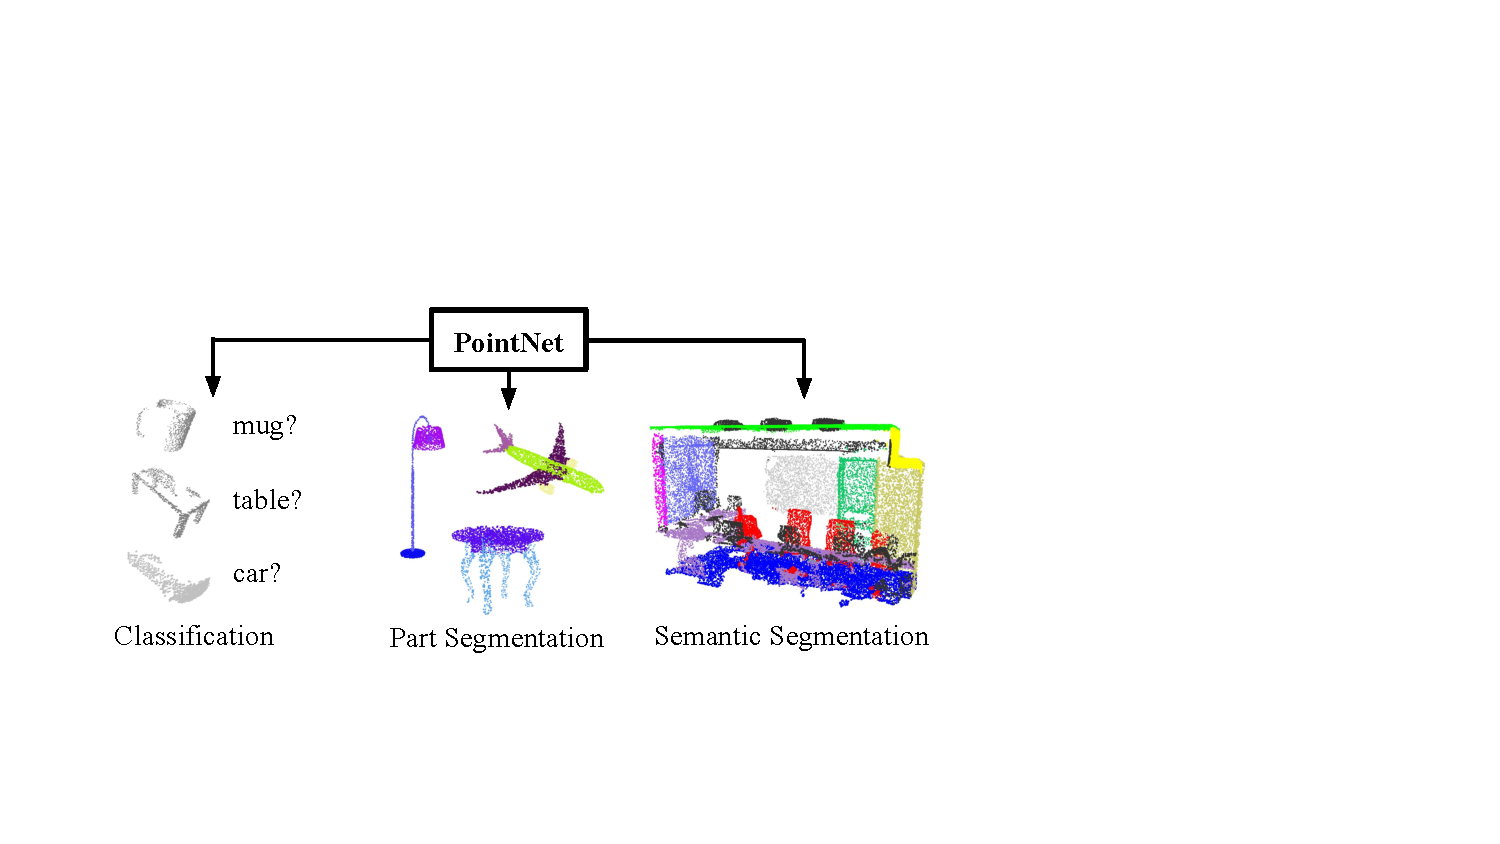
\includegraphics[width=\linewidth]{fig/teaser.pdf}
    \caption{\textbf{PointNet 的应用} 
    我们提出了一个新的神经网络结构,其输入为一个原始的点云(点的集合),没有经过体素化或预渲染。该网络具有一个统一的架构,能够学习全局和局部的点特征,从而为各种三维识别任务提供了一个简单、高速而有效的方法。 
    %We propose a novel deep net architecture that consumes raw point cloud (set of points) without voxelization or rendering. It is a unified architecture that learns both global and local point features, providing a simple, efficient and effective approach for a number of 3D recognition tasks.% 
    }
    \label{fig:teaser}
\end{figure}


\begin{figure*}[th!]
    \centering
    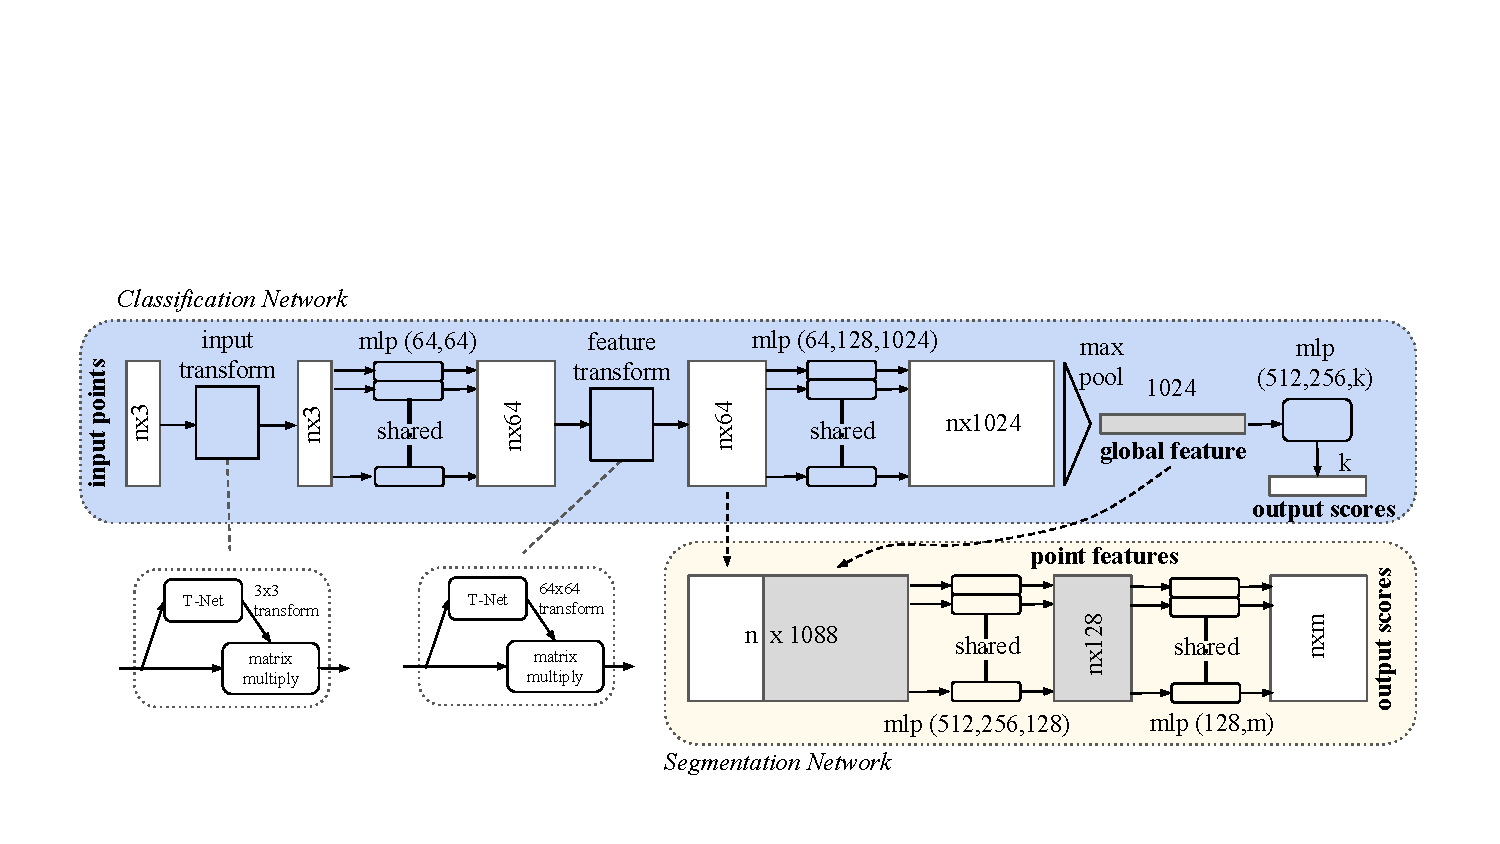
\includegraphics[width=0.9\linewidth]{fig/pointnet_fixed.pdf}
    \caption{\textbf{PointNet 架构}      分类网络将$n$个点作为输入,作用输入和特征变换,然后通过max pooling聚合点的特征,输出的是$k$种分类的分类分数。分割网络是分类网络的拓展,它连接局部和全局特征以及每个点输出的分数。``mlp''代表多层感知机,括号中的数字是层的大小。Batchnorm用于所有应用了ReLU的层。Dropout用于分类网络中的最后一个多层感知机。}
    \label{fig:pointnet_arch}
\end{figure*}

\section{相关工作}
\label{sec:related}
\begin{comment}
\todo{\\
  \paragraph{3d point cloud processing:}
  \begin{itemize}
    \item classification
    \item segmentation
    % \item correspondence
  \end{itemize} 
  traditionally, each 3d data processing task depends on some specific pipeline. our framework unifies them together.
  
  \paragraph{point cloud features:}
  \begin{itemize}
    \item global features
    \item local features
  \end{itemize}
  most works use hand-crafted features. 

  \paragraph{deep learning on 3d data:}
  \begin{itemize}
    \item multi-view CNN
    \item volumetric CNN
    \item spectral CNN on meshes 
    \item non end-to-end approach
  \end{itemize}
  in previous work of deep learning on point clouds, a point cloud is first converted to one of the above forms. however, there lacks work that directly operates on a raw point set.

  \paragraph{deep learning on unordered sets}
  \begin{itemize}
    \item discuss ``OrderMatters'', by Vinyals et al.
    \item say that this is a rather fundamental problem, related to many other tasks
  \end{itemize} 
}
\end{comment}

\paragraph{点云特征}
点云大部分的现有特征都是针对特定任务手工制作的。点特征通常编码某些统计特性,并且被设计成对于某些变换是不变的,这些变换通常被划分为内在的
\cite{aubry2011wave, sun2009concise, bronstein2010scale} 或外在的 ~\cite{rusu2008aligning, rusu2009fast, ling2007shape, johnson1999using, chen2003visual}。  它们还可以归类为局部特征和全局特征。对于特定任务,找到最优的特征组合并非易事。

%While one can extract all kinds of features and let a machine learning model decide which ones to use, the success of CNNs~\cite{lecun2015deep} for 2D images convinces us that an end-to-end feature learning paradigm is more promising. In this work we present a unified point feature learning network that can easily adapts to different tasks.

% \paragraph{Point Cloud Features}
% Most existing features for point cloud are handcrafted towards specific tasks. According to the spatial scopes, they can be categorized as local features and global features. Point features often encode certain statistical properties of points and are designed to be invariant to certain transformations, which are typically classified as being intrinsic [WKS, HKS] or extrinsic [PFH, FPFH, D2, spin image, LFD].

% Often one feature that works on task A may not perform well on task B. In addition, different features often make different assumptions of where the point cloud comes from. For example, HKS and WKS features work very well on organic objects such as human bodies, but they are not suitable for describing CAD models with combinatorial structures. For a specific task, it is not trivial to find the optimal feature combination for the task. 

% While one can extract all kinds of features and let a machine learning model to decide which ones to use, the success of CNNs [CITE] for 2D images convinces us that an end-to-end feature learning paradigm is more promising. In this work we present a unified point feature learning network that can easily adapts to different tasks, such as classification, segmentation, retrieval and correspondence. Our network directly works on point sets, due to its flexibility and broad usage in real applications.


\paragraph{3D数据的深度学习}
% \todo{we need to argue why point cloud (most close to raw sensor data), instead of meshes (not canonical), volume (sparsity), projected images (not in 3D, non-trivial to choose viewpoints) somewhere in the paper.}

3D数据具有多种流行的表示形式,从而有各种学习方法。
\emph{Volumetric CNNs:}~\cite{wu20153d, maturana2015voxnet, qi2016volumetric} 这是在体素形状上应用3D卷积神经网络的先驱。然而,由于数据的稀疏性和3D卷积的计算成本,体积表示受到其分辨率的限制。FPNN~\cite{li2016fpnn} 和 Vote3D~\cite{wang2015voting} 提出了处理稀疏性问题的特殊方法;然而,他们的操作仍然是在稀疏的体积上,处理非常大的点云对他们来说是一种挑战。
\emph{Multiview CNNs:}~\cite{su15mvcnn, qi2016volumetric} 试图将3D点云或形状渲染成2D图像,然后应用2D卷积神经网络对它们进行分类。通过精心设计的图像CNN,这一系列方法在形状分类和检索任务方面取得了突出的性能表现。~\cite{savvashrec}. 然而,将它们扩展到场景理解或其他3D任务例如点分类、形状完成上时表现很普通。
\emph{Spectral CNNs:} 最近的一些工作~\cite{bruna2013spectral, masci2015geodesic}在网格上使用了光谱CNN。但是这些方法目前受限于流形网格(例如有机物体),而且如何将它们扩展到非等距形状(例如家具)上并不明显。
\emph{Feature-based DNNs:}~\cite{fang20153d,guo20153d} 首先通过提取传统的形状特征将3D数据转换成向量,然后使用全连接网络对形状进行分类。我们认为它们受限于所提取特征的表示能力。

% In our work, we do deep learning directly on the raw 3D representation -- point clouds, without the pre-processing stage of converting them to volumes, images, graphs, or feature vectors. Therefore, our method has the potential to greatly simply the pipeline in practical usage.

% We argue that point cloud is a good representation in many aspects: 1) it's raw -- point clouds are the data acquired directly from depth sensors or laser scans, not like volumes or images that suffer from information loss. 2) it's in 3D, not like projected images that lack 3D geometry, which may require additional cross-view consistency mechanisms. 3) it's compact, not like volumetric grids that stores a 2D manifold surface in full 3D space. We design special networks to consume 3D point clouds and show that our network can be easily adapted for various 3D tasks with very good performance.


% Volumetric CNNs: [3DShapeNets, voxnet, our cvpr work] are the pioneers applying 3D convolutional neural networks on voxelized shapes. However, since sensors can only reach the surfaces of objects, most 3D data are just 2D manifold/surface living in a 3D space, thus volumetric grids are often sparse. Besides, the storage and computation cost both grow cubically with the input resolution. To address this challenge, [FPNN and vote3D] propose special methods to deal with the sparsity of volumetric representation; however, their operations are still performed on a very sparse volume and it is still challenging for them to process very large point clouds.

% Multiview CNNs: [MVCNN, our cvpr work, and some other image based methods] have tried to render 3D point cloud or shapes into 2D images and then apply 2D convolutional neural networks (using existing architectures such as AlexNet and VGG fine-tuned from ImageNet) to classify the shapes. With the well engineered image CNNs, this line of methods have achieved dominating performance on shape classification and retrieval tasks [cite SHREC]. However, it's nontrivial to extend them to scene understanding (not clear which camera positions to take), or other 3D tasks such as point classification and shape completion. Besides, when projecting 3D into images, we always have to convert predictions and data back and forth between 2D and 3D.

% Spectral CNNs: There has also been latest work that use spectral CNNs on meshes. However, these methods are currently constrained on manifold meshes such as organic objects and it's not obvious how to extend them to non-isometric shapes with sophisticated topological and geometric variations, such as furniture. Besides, acquiring meshes or point graphs require significant efforts in post processing from raw sensor data.

% Feature-based DNNs: [deep3dshape and Beihang's paper] firstly convert the 3D data into a vector, by extracting traditional shape features (HKS and WKS) and then use a fully connected neural network to classify the shape. We think they are constrained by the representation power of the features extracted.

% In our work, we do deep learning directly on the raw 3D representation -- point clouds, without the pre-processing stage of converting them to volumes, images, graphs, or feature vectors. Therefore, our method has the potential to greatly simply the pipeline in practical usage. We argue that point cloud is a good representation in many aspects: 1) it's raw -- point clouds are the data acquired directly from depth sensors or laser scans, not like volumes or images that suffer from information loss. 2) it's in 3D, not like projected images that lack 3D geometry, which may require additional cross-view consistency mechanisms. 3) it's compact, not like volumetric grids that stores a 2D manifold surface in full 3D space. We design special networks to consume 3D point clouds and show that our network can be easily adapted for various 3D tasks with very good performance.


\paragraph{无序集的深度学习}

从数据结构的角度来说,点云是无序的向量集合。当大部分深度学习工作集中在规则输入表示,如序列(语音和语言处理)、图像和体积(视频或3D数据)上时,很少有在点集上做深度学习工作的。

Oriol Vinyals等人最近的一项工作~\cite{vinyals2015order}研究了这个问题。他们使用具有注意机制的读取-处理-写入网络来处理无序输入集,同时展示他们的网络具有对数字进行排序的能力。然而,由于他们的工作重点是泛型集合和NLP应用,因此缺少了几何体在集合中的作用。

% Our work exploits the geometry properties in 3D point sets, provides theoretical analysis to what has been learned, gives rich visualizations to help understand the model. Our work also targets towards real applications of object classification and segmentation.

\section{问题陈述}
\label{sec:problem}
\begin{comment}
\todo{
  \begin{enumerate}
    \item we are interested in deep learning methods for object classification and segmentation on 3d point sets.
    \item we solve the two problems in a unified framework. in this framework, we use neural network to learn a function $f$ that takes a subset of points in $\R^3$ as input, and predicts the object recognition or per-point segmentation.  
  \end{enumerate}
}
\end{comment}

我们设计了一个能够将无序的点集作为输入的深度学习网络框架。一个点云可以由若干个三维点的集合表示 $\{P_i| \ i=1,...,n\}$,其中每个点 $P_i$ 都是其空间坐标 $(x,y,z)$ 和其他额外的特征频道(例如颜色、范数等)。出于简洁性和清晰性,除非特别指出,我们只使用三维空间坐标,即 $(x,y,z)$ 作为输入点的频道。

% We design a deep learning framework that directly consumes unordered point sets as inputs. %, while most recent state-of-the-art methods convert them to volumetric grids \cite{wu20153d,wang2015voting,qi2016volumetric} or projecting them to images \cite{su15mvcnn,qi2016volumetric}. % Furthermore, our proposed network is a unified framework for a various of applications including object classification, object-level part segmentation and scene semantic parsing. A point cloud is represented as a set of 3D points $\{P_i| \ i=1,...,n\}$, where each point $P_i$ is a vector of its $(x,y,z)$ coordinate plus extra feature channels such as color, normal etc. For simplicity and clarity, unless otherwise noted, we only use the $(x,y,z)$ coordinate as our point's channels. % Our network directly consumes the point cloud 

对于物品分类的任务,输入点可以直接采样自某一个形状,或是某个场景的点云预先分割好的结果。我们提出的深度网络为 $k$ 个候选分类输出 $k$ 个得分。对于语义分割任务,输入可以使一个用于零件部分分割的单个物体,也可以是一个 3D 场景下用于区域零件分隔的子空间。我们的模型将会为 $n$ 个点与 $m$ 个语义子分类输出  $n \times m$ 个得分。

% For the object classification task, the input point cloud is either directly sampled from a shape or pre-segmented from a scene point cloud. Our proposed deep network %first generate global descriptors for the whole input point cloud and then 
% outputs $k$ scores for all the $k$ candidate classes.
% For semantic segmentation, the input can be a single object for part region segmentation, or a sub-volume from a 3D scene for object region segmentation. Our model will output $n \times m$ scores for each of the $n$ points and each of the $m$ semantic sub-categories.



\section{点集上的深度学习}
我们提出的PointNet网络结构(\ref{sec:pointnet_arch}节)的灵感主要来源于\ref{sec:point_set_property}节所述的$\mathbb{R}^n$内点集的属性。 % We first describe the three properties in Sec~\ref{sec:point_set_property}; accordingly, we discuss our architecture designs in Sec~\ref{sec:pointnet_arch}, where we also summarize our whole network for classification and segmentation tasks. Furthermore, Sec~\ref{sec:theory} provides some theoretical analysis on how and why our network works well on point sets, though the architecture is not complicated.

\subsection{$\mathbb{R}^n$内点集的属性}
\label{sec:point_set_property}
网络的输入是来自欧几里得空间的点的子集,主要有一下三种主要的性质:

% \begin{itemize}
\bitem
\item 无序性。
不同于图片的像素或者立方体的体素,点云是一些无特定顺序的点的集合。换句话说,一个要处理$N$个3D点集的网络需要对按序输入的点集的$N!$种排序保持不变。 
\item 点之间有相互作用。这些点来自具有距离度量的空间。这意味着这些点不是孤立的,而且相邻的点形成一个具有意义的子集。因此,模型需要能够从邻近点中捕获局部结构,以及局部结构之间的组合相互作用。 
\item 转换的不变性。
作为一个几何体,已习得的点集表示需要对一些变换保持不变。例如,对一些点一起做旋转和平移变换既不会改变全局的点云类别、也不会改变点的分割。
\eitem
% \end{itemize}

% The above three properties of our input lead to the three key ideas of our network design, which are discussed respectively in the following section.


\subsection{PointNet的结构}
\label{sec:pointnet_arch}

我们的完整网络架构图如图\ref{fig:pointnet_arch}所示,其中用于分类的网络和用于分割的网络占据了网络结构中的很大一部分。请阅读图\ref{fig:pointnet_arch}的题注以了解流程。

我们的网络有三个关键模块:用作对称函数、聚类所有点的信息的最大池化层;一个局部和全局信息结合的结构;和两个对齐了输入点和点的特征的联合对齐网络。

我们将在以下的单独段落中讨论这些设计选择背后的原因。%, after a brief overview of the network.

% \paragraph{Overview} In basic PointNet: Given a point cloud input, for example, $n$ points of $(x,y,z)$ coordinates, the network firstly applies a function (multi-layer perceptron network) on each point independently. Function outputs across points are then aggregated with a max pooling layer. The aggregated vector is a global feature for the point cloud.
% 
% For classification task, the global feature is further passed through a few fully connected layers (with ReLU) to predict class scores for the entire point cloud.
% 
% For segmentation, we need to combine both local and global context for point class prediction. To this end, the global feature is appended to each point's local feature vector to provide a global context for individual point. We then apply a multi-layer perceptron net on the concatenated feature of each point to predict its class scores.
% 
% Additional input and feature space alignment network can be inserted, as shown in Fig~\ref{fig:pointnet_arch}. The alignment network is a regressor to transformation matrix and resembles the basic classification net in architecture.
% 

\paragraph{用于处理无序输入的对称函数}
为了使模型对输入排序不变,存在三种策略:1)将输入排列为规范顺序;2)将输入看作训练RNN的序列,但通过各种排列增加了训练数据;3)用一个简单的对称函数来聚类每个点的信息。这里,对称函数将$n$个向量作为输入,然后输出一个不受输入顺序变化影响的新向量。例如,$+$和$*$操作符是对称二元函数。 

尽管排序听起来像是一个简单的解决方法,但实际上谈及到一般意义上的点的扰动时,在高维空间中并不存在稳定的排序。这可以很容易地通过矛盾来显示。如果这样一种排序策略存在,那么它定义了高维空间和一维实线之间的双向映射。不难看出,谈及点扰动时要求排序的稳定等同在维度降低时保持映射在空间上的接近度,一般情况下这项任务是无法实现的。因此,排序并不能完全解决排序问题,而且因为排序问题的存在,网络很难学习到从输入到输出的一致映射。如实验(图\ref{fig:order_invariant})中所示,我们发现直接在排序点集上应用多层感知机的性能不好,尽管略优于直接处理无序输入。

使用RNN的方法是将点集作为顺序信号,并希望用随机排序的序列训练RNN,这样RNN将会变得和输入顺序无关。然而,在``OrderMatters''~\cite{vinyals2015order}中,作者已经证明顺序确实很重要而且无法完全被忽略。尽管RNN对于较短(几十个)的序列的输入排序已经具有相对良好的鲁棒性,但是很难扩展到像点集这样有成千上万的输入元素上。根据实验,我们也证明了基于RNN的模型在性能上不如我们所提出来的方法(图\ref{fig:order_invariant})。

我们的想法是通过对集合中转换元素应用对称函数来近似在点集上定义的一般函数:
\begin{align}
    f(\{x_1, \dots, x_n\})\approx g(h(x_1), \dots, h(x_n)),
    \label{eq:approx}
\end{align}
其中 $f:2^{\mathbb{R}^N} \rightarrow \mathbb{R}$, $h: \mathbb{R}^N\rightarrow \mathbb{R}^K$ 和 $g:\underbrace{\mathbb{R}^K\times \dots \times \mathbb{R}^K}_n \rightarrow \mathbb{R}$ 是对称函数。

根据实验,我们的基础模块十分简单:我们通过多层感知机来近似$h$,并通过单个变量函数和最大池化函数的组合来近似$g$。通过实验发现这样的模块结构表现的很好。通过$h$的集合,我们可以学到一些$f$来捕获点集的不同属性。 % This idea shares similar flavor with [cite leo's paper: probablistic shape fingerprint], where they define random functions on the input data and train a model based on the outputs of those optimization functions.  %Signature points are supposed to result in more extreme values for those random functions, thus the latter model can use weights to select them to make prediciton decisions for specific tasks. 
% In our architecture, instead of using random functions, we let the network itself learn a set of optimal functions to select signature points. 

尽管我们的关键模块看起来很简单,但它也具有很精彩的地方(参见\ref{sec:visualizing_pointnet}节),在一些不同的应用中能够表现出很强的性能(参见\ref{sec:application}节)。由于我们模块的简单性,我们也提供了\ref{sec:theory}节中的理论分析。


\paragraph{局部和全局信息聚类}
上一节的输出组成了一个向量$[f_1, \dots, f_K]$,这是输入集的全局标签。我们可以在形同全局特征上很容易训练SVM或多层感知机分类器以进行分类。然而,点的分割需要结合局部信息和全局信息。我们能够通过简单而高效的方式来实现这一目标。 % Even for global point classification, it could be beneficial to exploit more local geometries.

我们的解决方法可以在图\ref{fig:pointnet_arch}(\textit{Segmentation Network})中看到。在计算完全局点云特征向量后,我们将全局特征和每一个点的特征连接起来反馈给每一个点特征。然后我们基于组合的点特征提取新的每个点的特征,这样每个点特征都考虑了局部和全局信息。 % This structure can be repeated multiple times.

通过这样的修改,我们的网络能够预测依赖于局部几何和全局语义的每个点数量。例如我们可以准确地预测出每个点的法线(图中的补充),验证网络能够汇总来自该点的局部领域的信息。在实验环节中,我们也表明我们的模型可以在形状部分分割和场景分割方面实现最先进的性能。
    
\paragraph{联合对齐网络}
如果点云在经历了某些几何变换(比如刚性变换),那么点云的语义标签必须是不变的。因此我们希望已习得的点集表示不受这些变换影响。

一个自然的解决方法是在特征提取前将所有的输入集对齐到规范空间。Jaderberg等人~\cite{jaderberg2015spatial}介绍了一种通过采样和插值来对齐二维图像的空间变换的方法,通过在GPU上特别定制的层来实现。

与~\cite{jaderberg2015spatial}相比,我们的点云输入形式使我们能够以更简单的方式来实现这一目标。我们不需要发明任何新的层,也不需要像图像任务那样引入任何别名。我们通过一个小型网络(图~\ref{fig:pointnet_arch}中的T-net)预测仿射变换矩阵,并直接将该变换作用于输入点的坐标。这一小型网络本身类似于大型网络,由独立的点特征提取、最大池化和全连接层组成。更多关于T-net的细节将在附录中介绍。

这个想法可以进一步扩展到特征空间的对齐。我们可以在点的特征上插入另一个对齐网络,并预测特征变换矩阵以对齐来自不同输入点云的特征。然而,特征空间中的变换矩阵比空间变换矩阵的维度高很多,这极大地增加了优化的难度。因此,我们在softmax的训练损失中增加了一个正则化项。我们约束特征变换矩阵接近于正交矩阵:
\begin{equation}
    L_{reg} = \|I - AA^T\|_F^2,
\end{equation}
其中$A$是小型网络预测得到的特征对齐矩阵。正如我们所期待的,一个正交变换将不会损失任何输入的信息。我们发现通过增加正则化项,优化变得更加稳定,而且我们的模型实现了更好的性能。


\subsection{理论分析}
\label{sec:theory}
 
% \todo{
%   goal: show that this network is theoretically robust to perturbation and corruption (additional points and incompleteness) of input data.
%   \begin{itemize}
%     \item analyze the max pooling layer: it selects a finite set of key points. the cardinality of the key point set is constrained by the dimension of max pooling. 
%     \item add some understanding of the symmetry function, if we can
%   \end{itemize}
% }

\paragraph{通用近似性} 

我们首先展示我们的神经网络具备通用近似到连续的集合函数上的能力。由于集函数的连续性,直观上我们认为,一个输入点集上的微小扰动不应当引起函数值的剧烈变化,例如其分类任务或分割任务的表现分数。

%We first show the universal approximation ability of our neural network to continuous set functions. By the continuity of set functions, intuitively, a small perturbation to the input point set should not greatly change the function values, such as classification or segmentation scores.

形式化地, 令 $\mathcal{X}=\{S: S\subseteq [0,1]^m \text{ and } |S|=n\}$,   $f:\mathcal{X}\rightarrow \mathbb{R}$ 在 $\mathcal{X}$ 上关于赫斯多夫距离 $d_H(\cdot, \cdot)$ (即: $\forall \epsilon > 0, \exists \delta >0$, for any $S, S'\in\mathcal{X}$, if $d_H(S, S') < \delta$, 则有 $|f(S)-f(S')|< \epsilon$)的连续的集函数。 我们的理论认为在池化层给定足够多的神经元, $f$ 能被无限近似,即, 在 \eqref{eq:approx} 中的 $K$ 
已经足够大。

% Formally, let $\mathcal{X}=\{S: S\subseteq [0,1]^m \text{ and } |S|=n\}$,   $f:\mathcal{X}\rightarrow \mathbb{R}$ is a continuous set function on $\mathcal{X}$ w.r.t to Hausdorff distance $d_H(\cdot, \cdot)$, i.e., $\forall \epsilon > 0, \exists \delta >0$, for any $S, S'\in\mathcal{X}$, if $d_H(S, S') < \delta$, then $|f(S)-f(S')|< \epsilon$. Our theorem says that $f$ can be arbitrarily approximated by our network given enough neurons at the max pooling layer, i.e., $K$ in \eqref{eq:approx} is sufficiently large. 

\begin{theorem}

令 $f:\mathcal{X}\rightarrow \mathbb{R}$ 是一个关于赫斯多夫距离 $d_H(\cdot, \cdot)$ 的集函数。$\forall \epsilon > 0$, $\exists$ 一个连续函数 $h$ 和一个对称函数 $g(x_1, \dots, x_n)=\gamma \circ \mbox{MAX}$, 使得任意 $S\in\mathcal{X}$,

% Suppose $f:\mathcal{X}\rightarrow \mathbb{R}$ is a continuous set function w.r.t Hausdorff distance $d_H(\cdot, \cdot)$. $\forall \epsilon > 0$, $\exists$ a continuous function $h$ and a symmetric function $g(x_1, \dots, x_n)=\gamma \circ \mbox{MAX}$, such that for any $S\in\mathcal{X}$,


\begin{align*}
	\left|f(S) - \gamma\left(\underset{x_i\in S}{\mbox{MAX}}\left\{h(x_i)\right\}\right)\right| < \epsilon
\end{align*}

其中 $x_1, \ldots, x_n$ 是一系列在 $S$ 中任意顺序排列的元素,$\gamma$ 是一个连续函数, 且 $\mbox{MAX}$ 是一个取 $n$ 个向量最为输入,然后返回一个元素层面上的最大值的最大化向量运算符。

\end{theorem}

该定理的理论证明参见本文的附加材料。其主要思想是,在最差情况下,通过将空间划分成等体积的体素,网络的学习结果是到将点云转换为体积表示。而在实际情况下,网络会学习一个聪明得多的策略来探测空间,正如我们将在点函数的可视化中呈现的那样。

% The proof to this theorem can be found in our supplementary material. The key idea is that in the worst case the network can learn to convert a point cloud into a volumetric representation, by partitioning the space into equal-sized voxels. In practice, however, the network learns a much smarter strategy to probe the space, as we shall see in point function visualizations.

\begin{figure}[t!]
    \centering
    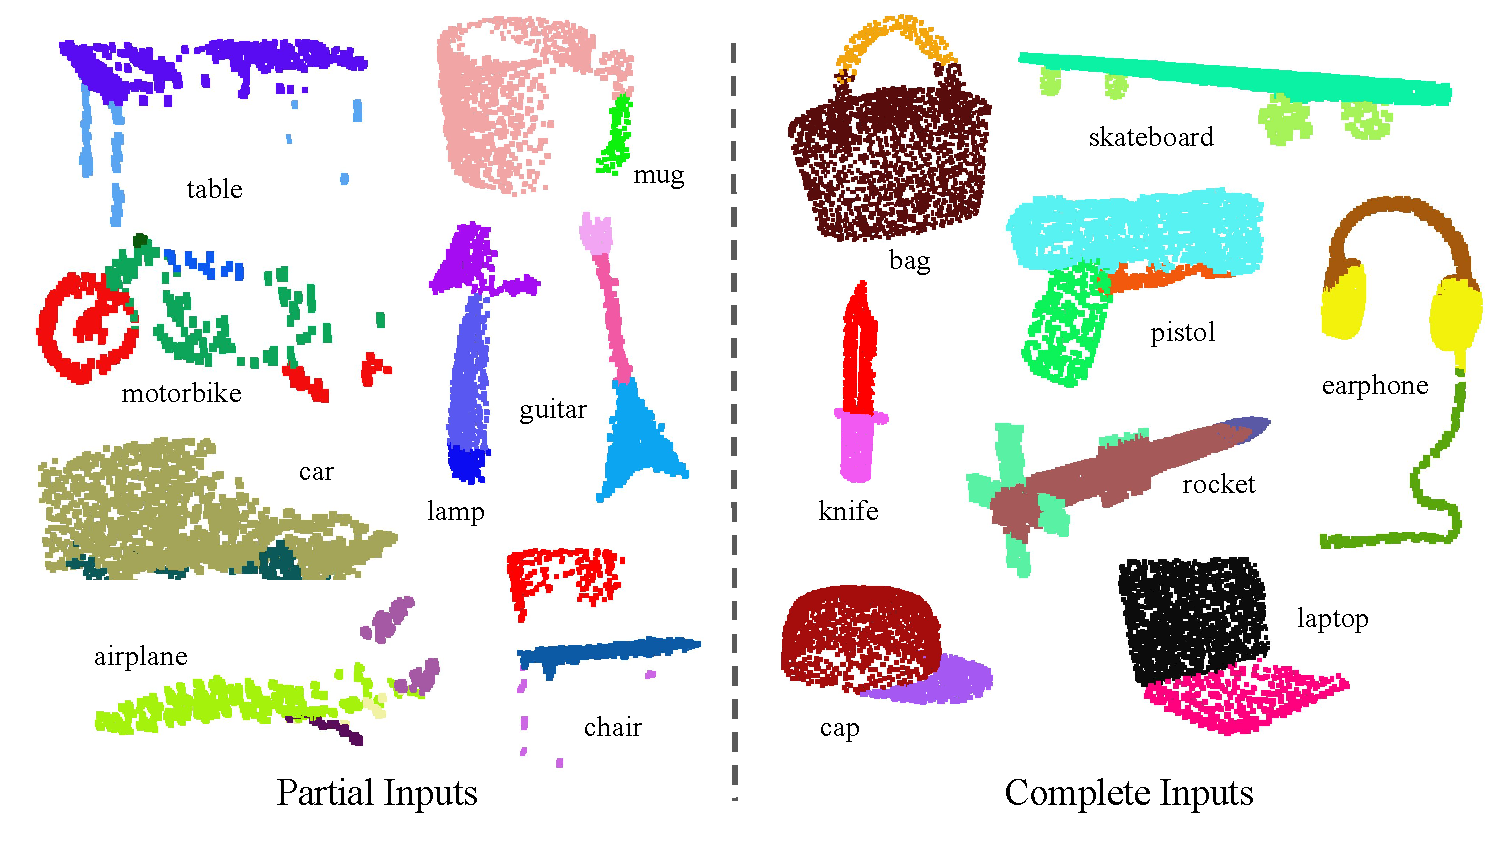
\includegraphics[width=0.8\linewidth]{fig/segres.pdf}
    \caption{
        \textbf{零件分割的量化结果} 我们可视化了横跨 16 个分类的 CAD 零件的分割结构。我们分别展示了部分模拟的 Kinect 扫描结果(左)和完全的 ShapeNet CAD 模型的结果(右)。
  %  \textbf{Qualitative results for part segmentation.} We visualize the CAD part segmentation results across all 16 object categories. We show both results for partial simulated Kinect scans (left block) and complete ShapeNet CAD models (right block).
    }
    \label{fig:qualitative_part_segmentation}
\end{figure}

\paragraph{瓶颈维度与稳定性} 从理论上和实践上,我们发现我们网络的表达性收到池化层维度的强烈影响。即,\eqref{eq:approx} 中的 $K$。在此我们提供了一个分析,同时也揭示了与我们模型的稳定性相关的一些属性。  

% \paragraph{Bottlenet dimension and stability} Theoretically and experimentally we find that the expressiveness of our network is strongly affected by the dimension of the max pooling layer, i.e., $K$ in \eqref{eq:approx}. Here we provide an analysis, which also reveals properties related to the stability of our model. 

我们定义 $\myvec u=\underset{x_i\in S}{\mbox{MAX}}\{h(x_i)\}$ 为网络 $f$ 的子网络。其中 $f$ 将分布在  $[0,1]^m$ 中的点集映射到了 $K$ 维空间的向量。接下来的理论分析指出,输入中的微小扰动或额外的噪音点不会严重影响我们网络的输出结果。

%We define $\myvec u=\underset{x_i\in S}{\mbox{MAX}}\{h(x_i)\}$ to be the sub-network of $f$ which maps a point set in $[0,1]^m$ to a $K$-dimensional vector. The following theorem tells us that small corruptions or extra noise points in the input set are not likely to change the output of our network:

\begin{theorem}

令 $\myvec u:\mathcal{X}\rightarrow \mathbb{R}^K$ 使得 $\myvec u=\underset{x_i\in S}{\mbox{MAX}}\{h(x_i)\}$ 且 $f=\gamma \circ \myvec u$. 则, 

% Suppose $\myvec u:\mathcal{X}\rightarrow \mathbb{R}^K$ such that $\myvec u=\underset{x_i\in S}{\mbox{MAX}}\{h(x_i)\}$ and $f=\gamma \circ \myvec u$. Then, 

\begin{enumerate}[label=(\alph*)]   

    \item $\forall S, \exists~\mathcal{C}_S, \mathcal{N}_S\subseteq \mathcal{X}$,  $f(T)=f(S)$ if  $\mathcal{C}_S\subseteq T\subseteq \mathcal{N}_S$;
    %\item Define the equivalence relation $\sim$ as $S\sim S'$ if $\myvec u(S)=\myvec u(S')$, then $\mathcal{C}_S=\underset{S'\sim S}{\cap} S'$ and $\mathcal{N}_S=\underset{S'\sim S}{\cup} S'$.
    % \item Let $S\sim S'$ if $\myvec u(S)=\myvec u(S')$. $\mathcal{C}_S=\underset{S'\sim S}{\cap} S'$, $\mathcal{N}_S=\underset{S'\sim S}{\cup} S'$.
    \item $|\mathcal{C}_S| \le K$
\end{enumerate}
\label{thm:thm2}
%     \begin{itemize}            
%     \item Critical points.
%     \\$\mathbb{C}=\{x_i: \myvec u_j(S)=h_j(x_i) \mbox{ for some } 1\le j\le K\}\cap S$
%     \item Free-space points.
%     \\$\mathbb{F}=\{x_i: \myvec u_j(S)<h_j(x_i) \mbox{ for some } 1\le j\le K\}\cap S$
%     \item Non-critical points. 
%     \\$\mathbb{N}=\{x_i: \myvec u_j(S)>h_j(x_i) \mbox{ for some } 1\le j\le K\}\cap S$
% For any $S'$ such that  $\mathbb{C} \subseteq S' \subseteq \mathbb{C}\cup\mathbb{N}$, $\myvec u(S')\equiv \myvec u(S)$; for any $S'$ such that $S'\cap \mathbb{F}\neq \emptyset$, $\myvec u(S')\neq \myvec u(S)$.
%\end{itemize}
\end{theorem}

关于上述定理,我们进一步阐释其推论。(a) 说明 $f(S)$ 在针对输入干扰时保持不变,只要  $\mathcal{C}_S$ 中的点被保留。同时也不会受到在 $\mathcal{N}_S$ 以内的额外噪声点的影响。(b) 说明 $\mathcal{C}_S$ 只包含一些有限数量的点,取决于 \eqref{eq:approx} 中的 $K$。换句话说,$f(S)$ 事实上是完全由一个元素数量小于或等于 $K$ 的有限子集 $\mathcal{C}_S\subseteq S$决定的。因此,我们将 $\mathcal{C}_S$ 称为 $S$ 的 \emph{关键点集},将 $K$ 成为 $f$ 的 \emph{瓶颈维度}。

% We explain the implications of the theorem. (a) says that $f(S)$ is unchanged up to the input corruption if all points in $\mathcal{C}_S$ are preserved; it is also unchanged with extra noise points up to $\mathcal{N}_S$. (b) says that $\mathcal{C}_S$ only contains a bounded number of points, determined by $K$ in \eqref{eq:approx}. In other words, $f(S)$ is in fact totally determined by a finite subset $\mathcal{C}_S\subseteq S$ of less or equal to $K$ elements. We therefore call $\mathcal{C}_S$ the \emph{critical point set} of $S$ and $K$ the \emph{bottleneck dimension} of $f$. 

结合 $h$ 的连续性,我们的模型关于点的扰动、缺失或额外的噪声点的健壮性得以解释。其健壮性的提升类似于机器学习模型中的稀疏原则。\textbf{直观上看,我们的模型能够通过一个稀疏的关键点来概括出形状。}在实验部分,我们可以看到从一个物体骨架的关键点。

% Combined with the continuity of $h$, this explains the robustness of our model w.r.t point perturbation, corruption and extra noise points. The robustness is gained in analogy to the sparsity principle in machine learning models. {\bf  Intuitively, our network learns to summarize a shape by a sparse set of key points.} In experiment section we see that the key points form the skeleton of an object.




\begin{comment}
\subsection{The properties of point sets in $\R^n$}
\todo{
  our input is a subset of points from a Euclidean space. It has three main properties:
  \begin{itemize}
    \item as a set, points in it has no order; 
    \item the points are from a metric space. therefore, local structures from near points have to be characterized;
    \item as a geometric object, the learned representation of the point set should be invariant to certain transformations.
  \end{itemize}
  the above three properties of our input leads to the three key ideas of our network design. we explain one by one.
}
\subsection{Unordered point set as input}
\todo{
  \begin{itemize}
    \item three strategies exist: 1) sorting input into a canonical order; 2)  use RNN but train order-invariantly; 3) use a symmetric function to aggregate the information from each point. 
    \item theoretically and empirically argue that the first two choices are not good. 
    \item our idea is to approximate a general function defined on a point set by applying a symmetric function on transformed elements in the set: $$f(\{x_1, \dots, x_n\})\approx g(h(x_1), \dots, h(x_n)),$$ where $f:2^{\R^N} \rightarrow \R$, $h: \R^N\rightarrow \R$ and $g:\R\times \dots \times \R\rightarrow \R$ is a symmetric function.
    \item we think this is provable for some good $f$.
    \item empirically, we approximate $h$ by a multi-layer perceptron network and $g$ by a composition of a single variable function and a max pooling function. this is found to work well by experiments.
    \item we can learn a number of $f$'s to capture different properties of the set.
  \end{itemize}
}

\subsection{Local and global information aggregation}
\todo{
  \begin{itemize}
    \item the output from the above section forms a vector $[f_1, \dots, f_M]$, which is a global signature of the input set.
    \item however, for tasks such as segmentation, we also need combine local information and global information. 
    \item xxx
  \end{itemize}
}

\subsection{Input and feature space alignment}
\todo{
  \begin{itemize}
    \item as we explained earlier, the learned representation of the point set should be invariant to certain transformations.
    \item we propose to apply an input dependent transformation for each instance to align all input set to a canonical space
    \item the input of our data are very friendly to geometric transformations, such as affine. we can therefore predict the transformation matrix by a neural network, named Joint Alignment Network.
    \item this idea can be extended to the alignment of feature space, as well
  \end{itemize} 
}

\subsection{PointNet architecture}
\todo{
  \begin{itemize}
    \item we implement the above ideas into a network for point set learning, named PointNet
    \item show the network for classification and explain 
    \item show the network for segmentation and explain
  \end{itemize}
}

\subsection{Theoretical Analysis}
\todo{
  goal: show that this network is theoretically robust to perturbation and corruption (additional points and incompleteness) of input data.
  \begin{itemize}
    \item analyze the max pooling layer: it selects a finite set of key points. the cardinality of the key point set is constrained by the dimension of max pooling. 
    \item add some understanding of the symmetry function, if we can
  \end{itemize}
}



\end{comment}

\section{实验}
\begin{table}[t!]
    \small
    \centering
    \begin{tabular}[width=\linewidth]{l|c|c|c|c}
    \hline
    ~               & input        & \#views    & accuracy & accuracy \\ 
    ~ & & & avg. class & overall \\ \hline
    SPH~\cite{kazhdan2003rotation}             & mesh        & - & 68.2         & -  \\ \hline
    3DShapeNets~\cite{wu20153d}     & volume       & 1        & 77.3  & 84.7 \\
    VoxNet~\cite{maturana2015voxnet}          & volume       & 12        & 83.0 & 85.9 \\
    Subvolume~\cite{qi2016volumetric}    & volume       & 20      & 86.0  & \textbf{89.2} \\ \hline
    LFD~\cite{wu20153d}             & image        & 10        & 75.5 & -\\
    MVCNN~\cite{su15mvcnn}           & image        & 80        & \textbf{90.1} & -\\ \hline
    Ours baseline  & point    & -     & 72.6  & 77.4\\
    Ours PointNet   & point   & 1        & 86.2 & \textbf{89.2} \\ \hline
    \end{tabular}
    \caption{\textbf{ModelNet40上的分类结果} 我们的网络在一系列3D输入的深度网络中达到最先进的效果。}
    \label{tab:classification}
\end{table}
\label{sec:exp}
实验被分成了四部分。首先,我们展示了PointNets可以应用于多个3D识别任务 (Sec~\ref{sec:application})。 其次,我们提供了详细的实验来验证我们的网络设计 (Sec~\ref{sec:arch_analysis})。最后,我们可视化了网络学到的内容 (Sec~\ref{sec:visualizing_pointnet}) 并且分析了时间和空间复杂度 (Sec~\ref{sec:complexity})。



\begin{table*}[th!]
    \small
    \centering
    \begin{tabular}[width=\linewidth]{l|c|p{0.5cm}p{0.4cm}p{0.4cm}p{0.4cm}p{0.5cm}p{0.6cm}p{0.5cm}p{0.5cm}p{0.5cm}p{0.6cm}p{0.6cm}p{0.3cm}p{0.5cm}p{0.6cm}p{0.6cm}p{0.6cm}}
    \hline
    ~        & mean & aero & bag & cap & car & chair & ear & guitar & knife & lamp & laptop & motor & mug & pistol & rocket & skate & table \\ 
    &   & &  &  &  &  & phone &  &   &  &  & &    &    &    & board &  \\ \hline
    \# shapes & & 2690 & 76 & 55 & 898 & 3758 & 69 & 787 & 392 & 1547 & 451 & 202 & 184 & 283 & 66 & 152 & 5271 \\ \hline
    Wu~\cite{Wu2014248} &  -  & 63.2  & - &      -    & -   & 73.5 & - &    - &    - &     74.4  & -    & - &   -   &   -   &   - & -  &  74.8 \\
    Yi~\cite{Yi16} & 81.4 & 81.0 & 78.4 & 77.7 & \textbf{75.7} & 87.6 & 61.9 & \textbf{92.0} & 85.4 & \textbf{82.5} & \textbf{95.7} & \textbf{70.6} & 91.9 & \textbf{85.9} & 53.1 & 69.8 & 75.3 \\ \hline
    3DCNN & 79.4 & 75.1 & 72.8 & 73.3 & 70.0 & 87.2 & 63.5 & 88.4 & 79.6 & 74.4 & 93.9 & 58.7 & 91.8 & 76.4 & 51.2 & 65.3 & 77.1 \\ 
    Ours & \textbf{83.7} & \textbf{83.4} & \textbf{78.7} & \textbf{82.5} & 74.9 & \textbf{89.6} & \textbf{73.0} & 91.5 & \textbf{85.9} & 80.8 & 95.3 & 65.2 & \textbf{93.0} & 81.2 & \textbf{57.9} & \textbf{72.8} & \textbf{80.6} \\ \hline
    \end{tabular}
    \caption{\textbf{ShapeNet数据集上的分割结果} 评价指标是点集的mIoU(\%)。 我们与两种传统方法 \cite{Wu2014248} \cite{Wu2014248} 以及我们提出的三维卷积网络对比。PointNet方法在mIoU上达到最佳表现。}
    %Notice that while all the other three methods are tested on the official ShapeNet train/validation/test split~\cite{shapenet2015}, the statistics for Wu's method~\cite{Wu2014248} are tested on a much larger set of shapes.
    \label{tab:segmentation}
\end{table*}



\subsection{应用}
\label{sec:application}
在本节中,我们将展示我们的网络是如何经过训练,来完成3D目标分类、目标零件分割和场景语义分割任务\footnote{更多应用样例,例如形状对应和基于点云的CAD模型检索包含在补充资料中。} 即使我们基于全新的数据表示(点集)进行研究,我们也能够在多个任务的基准测试中获得相当的甚至更好的性能。

\paragraph{3D目标分类} 我们的网络学习了可用于目标分类的全局点云特征。我们在ModelNet40~\cite{wu20153d} 形状分类基准上评估了我们的模型。总共有来自40个人造目标类别的12311个CAD模型,分为用于训练的9843个和用于测试的1468个。以前的方法主要集中于体积和多视图图像表示,我们提出了第一个直接处理原始点云的方法。

我们根据表面区域在网格面上均匀地采样了1024个点并将它们归一化为一个单位球体。在训练过程中,我们还通过沿上轴随机旋转对象并使用均值为0和标准差为0.02的高斯噪声抖动每个点的位置来动态地增强点云。


在表~\ref{tab:classification}中,我们将我们的模型与以前的相关工作,以及我们基于从点云中提取的传统特征(点密度、D2、形状轮廓等)MLP的基准线进行比较。我们的模型在基于3D输入(体积和点云)的所有方法中实现了最优的性能。仅仅使用全连接层和最大池化,我们的网络在推理速度上获得了强大的领先优势,并且也可以很容易地在CPU中并行化。但我们的方法与基于多视图的方法 (MVCNN~\cite{su15mvcnn}),之间仍然存在一点小差距,我们认为这是精细几何细节的丢失导致的,而这些细节可以被渲染图像所捕获。

\paragraph{3D目标零件分割} 零件分割是一项具有挑战性的细粒度3D识别任务。给定3D扫描或网格模型,任务是为每个点或面分配所属部分类别标签(例如椅子腿、杯柄)。
%The segmentation results are strong cues for part detection systems, which are key to many robotics applications such as grasping and affordance reasoning.

%Part segmentation requires knowledge of both local geometric and global semantics knowledge. By aggregating global feature vector to our point feature, our network is able to learn a \emph{deep point descriptor} that considers both local and global context, which suits well for this task.

我们对来自~\cite{Yi16}的ShapeNet部分数据集进行评估,其中包含来自16个类别的16881个形状,总共标注了50个部分。大多数目标类别都标有两到五个部分。对应的真实标签注释标记在形状上的采样点上。

我们将零件分割制定转换为每点分类问题。评估指标是点上的mIoU。对于类别C的每个形状S,计算形状的mIoU:对于类别C中的每个部分类型,计算真实和预测之间的IoU。如果真实点和预测点的并集为空,则将一部分IoU计为1。然后我们对类别C中所有部分类型的IoU进行平均以获得该形状的mIoU。为了计算类别的mIoU,我们取该类别中所有形状的mIoU的平均值。

在本节中,我们将我们的分割版PointNet (图~\ref{fig:pointnet_arch}的修改版, \textit{分割网络}) 和两种均利用了逐点几何特征和形状之间的对应关系的传统方法 \cite{Wu2014248} 和 \cite{Yi16} ,以及我们自有的3DCNN基准线进行了比较。有关3DCNN的详细修改和网络架构,请参阅补充说明。
%We design the segmentation 3D CNN architecture as a fully convolutional one that keeps volume size through all layers. In the end each voxel has a receptive field of 19 voxels with spatial resolution of 32.

在表~\ref{tab:segmentation}, 我们报告了每个类别和平均IoU(\%) 分数。我们观察到平均IoU有2.3\% 的提高,并且我们的网络在大多数类别中都优于基准方法。


\begin{table}[b!]
    \centering
    \small
    \begin{tabular}[width=\linewidth]{l|c|c}
    \hline
    ~             & mean IoU  & overall accuracy \\ \hline
    Ours baseline          &  20.12 & 53.19    \\ \hline
    Ours PointNet          & \textbf{47.71} & \textbf{78.62}  \\ \hline
    \end{tabular}
    \caption{\textbf{场景语义分割结果} 评价指标是13个类(结构和家具加上其他)的平均IoU和根据点集计算的分类准确率。 }
    \label{tab:semantic_segmentation}
\end{table}

\begin{table}[b!]
    \centering
    \small
    \begin{tabular}[width=\linewidth]{l|cccc|c}
    \hline
    ~                              & table & chair & sofa & board & mean  \\ \hline
    \# instance & 455 & 1363 & 55 & 137 & ~ \\ \hline
    Armeni et al.~\cite{armeni_cvpr16}          & 46.02 & 16.15 & \textbf{6.78} & 3.91  & 18.22 \\ \hline
    Ours & \textbf{46.67}     & \textbf{33.80 }    & 4.76    & \textbf{11.72}     & \textbf{24.24}     \\ \hline
    \end{tabular}
    \caption{\textbf{场景中3D物体检测结果} 评价指标是3D体积块中IoU阈值为0.5的平均准确率。}
    \label{tab:3d_detection}
\end{table}


% Move to supp
% While \cite{Wu2014248} and \cite{Yi16} deal with each object category independently, due to the lack of training data for some categories (the total number of shapes for all the categories in the data set are shown in the first line), we train our PointNet and the 3D volumetric CNN baseline across categories. To allow fair comparison, when testing these two models, we only predict part labels for the given specific object category. 

我们还对模拟Kinect扫描的任务进行了实验,来测试这些方法的稳健性。 对于ShapeNet部分数据集中的每个CAD模型,我们使用BlensorKinectSimulator~\cite{Gschwandtner11b} 从六个随机视点生成不完整的点云。我们根据这些完整形状和部分扫描数据,使用相同的网络架构和训练设置训练我们的PointNet。 结果表明,我们仅损失了5.3\%的平均IoU。 在图~\ref{fig:qualitative_part_segmentation}中,我们展示了针对完整数据和部分数据的定性结果。可以看到,虽然仅提供部分数据的任务相当具有挑战性,但我们的对其的预测是合理的。
%Since most real world scans are very partial due to occlusions, a model's robustness to partial input is key to evaluate its value in practice.


%From complete to partial input, we observed a $5.3\%$ mIoU drop. It is reasonable since lots of points are missed in virtual scans -- more structures need to be inferred. Still our model can segment well in some surprisingly partial cases, as shown in Fig~\ref{fig:qualitative_part_segmentation}, where both results on complete and partial data are displayed.

\begin{comment}
\begin{table}[h!]
    \small
    \centering
    \begin{tabular}[width=\linewidth]{l|cccc}
    \hline
    ~ & complete input & partial input \\ \hline
    3D CNN & 75.3 & 69.7 \\ \hline
    Ours PointNet & \textbf{80.6} & \textbf{75.3}  \\ \hline
    \end{tabular}
    \caption{\textbf{Segmentation results on partial scans.} Metric is mean IoU across all shapes.}
    %We perform rotation augmentation when training our PointNet on complete data to fairly compare with the simulated Kinect scans, that are generated from multiple perspective. In Table~\ref{tab:segmentation}, however, to compare with the traditional methods that rely on global orientation of shapes, no rotation augmentation is performed there.
    \label{tab:segmentation_partial}
\end{table}
\end{comment}

\paragraph{场景语义分割} 我们的零件分割网络可以很容易地扩展到语义场景分割,其中点标签成为语义目标类别,而不是目标的部分标签。
%Similar to image segmentation, we propose a 3D semantic segmentation task that organizes 3D points into semantic categories.

%Since our network operates on raw points, we can directly classify each point. On other hand, volumetric CNN and image based methods have to convert results back and forth in different representations.

% \begin{comment}
% Based on our net's ability to learn to classify 3D objects and segment point cloud, we can further achieve 3D object detection in scenes.
% \end{comment}

我们在斯坦福3D语义解析数据~\cite{armeni_cvpr16}上进行了实验。该数据集包含来自Matterport扫描仪的3D扫描结果,有6个大型室内区域组成,总共包括271个房间。扫描中的每个点都用来自13个类别(椅子、桌子、地板、墙壁等以及杂物)的语义标签中的一个进行注释。

为了准备训练数据,我们首先按房间分割点,然后将房间采样为面积为1mx1m的块。我们训练PointNet的分割版来预测每个块中的每个点类。每个点由XYZ、RGB和基于房间的归一化位置(从0到1)的9维向量表示。在训练时,我们实时的从每个块中随机采样4096个点。在测试时,我们对所有点进行测试。我们遵循与~\cite{armeni_cvpr16} 相同的协议,使用k-fold策略进行训练和测试。
%The sampled blocks have a overlap of half a meter. 


我们将我们的方法与使用人工设计点特征的基准线进行比较。基准线提取相同的9维局部特征和三个额外特征:局部点密度、局部曲率和法线。 我们使用标准MLP作为分类器。结果如表~\ref{tab:semantic_segmentation}所示,其中我们的PointNet方法明显优于基准线方法。 在图~\ref{fig:qualitative_segmentation}中,我们展示了定性分割结果。我们的网络能够输出平滑的预测,并且对缺失点和遮挡具有鲁棒性。




基于我们网络的语义分割输出,我们进一步构建了一个使用连接的组件进行目标采样的3D目标检测系统(有关详细信息,请参阅补充说明)。我们在表~\ref{tab:3d_detection}中与之前最先进的方法进行了比较。之前的方法基于滑动形状方法(带有CRF后处理),这种方法使用的支持向量机针对体素网格中的局部几何特征和全局房间上下文特征进行训练。我们的方法在所报告的家具类别上的效果大大优于它。

%we build a simple 3D object detection system. We use connected component with segmentation scores to get object proposals in scenes. For each proposed object, it's detection score is computed as the average point score for that category. Proposals with too less points or too small areas/volumes are pruned before evaluation. We observe that in some rooms such as auditoriums lots of objects (e.g. chairs) are close to each other, where connected component would fail to correctly segment out individual ones. Therefore we leverage our classification network and uses sliding shape method to alleviate the problem. The proposed boxes from connected component and sliding shapes are combined for final evaluation~\footnote{See supplementary for more details on implementation.}.



\begin{figure}[t!]
    \centering
    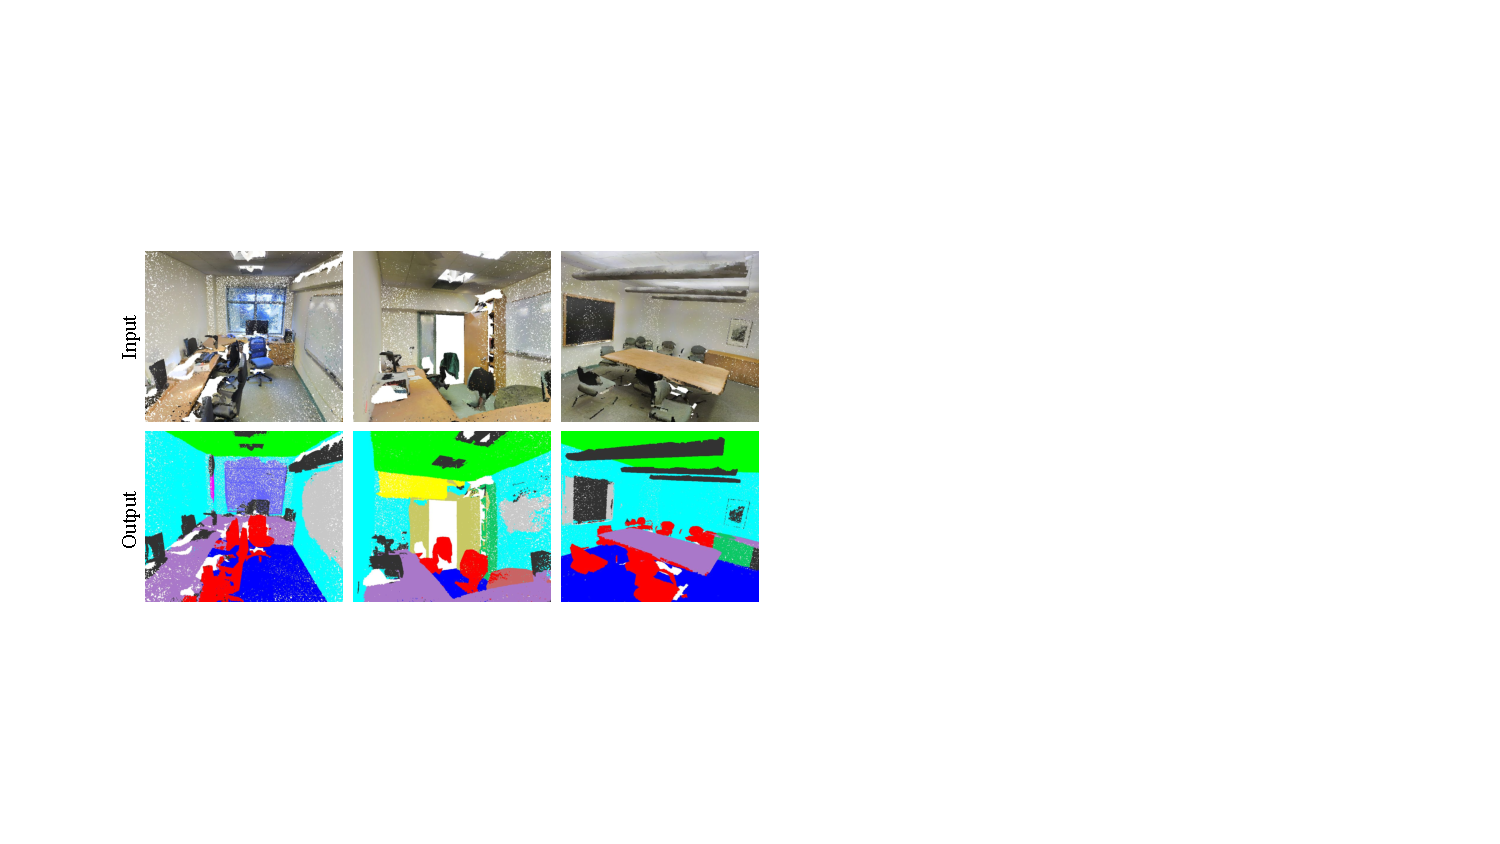
\includegraphics[width=0.8\linewidth,height=4cm]{fig/semantic}
    \caption{\textbf{语义分割的定性结果} 上一行是带颜色纹理的点云。底下是输出的语义分割结果(以点云展示),输出结果展示同输入的相机角度一致。}
    \label{fig:qualitative_segmentation}
\end{figure}

\subsection{架构设计分析}
\label{sec:arch_analysis}

在本节中,我们通过控制验证我们的设计选择实验。我们还展示了我们网络超参数的影响。
%~\footnote{Due to the limit of space, we refer the analysis on bottleneck dimension and number of input points to supplementary.}


\paragraph{与替代顺序不变方法的比较} 如第~\ref{sec:pointnet_arch}节所述,至少有三种选择可用于使用无序集合输入。我们使用ModelNet40形状分类问题作为测试平台来比较这些选项,以下两个控制实验也将使用此任务。

我们比较的基准线 (如图~\ref{fig:order_invariant}所示)包括:未排序和已排序的 $n \times 3$ 数组的多层感知机,将输入点视为序列的RNN模型,以及基于对称函数的模型。我们实验的对称操作包括最大池化、平均池化和基于注意力的加权和。注意方法类似于~\cite{vinyals2015order}中的方法,即从每个点特征预测一个标量分数,然后通过计算softmax跨点对分数进行归一化。然后根据归一化分数和点特征计算加权和。如图~\ref{fig:order_invariant}所示,最大池化操作以较大的优势幅度实现了最佳性能,这验证了我们的选择。


% \begin{table}
%     \small
%     \centering
%     \begin{tabular}[width=\linewidth]{l|c}
%     \hline
%     ~                    & accuracy \\ \hline
%     MLP (unsorted input) & 24.2       \\
%     MLP (sorted input)   & 45.0       \\
%     LSTM                 & 78.5       \\ \hline
%     Attention sum        & 83.0       \\
%     Average pooling      & 83.8       \\
%     Max pooling          & \textbf{87.1}       \\ \hline
%     \end{tabular}
%     \caption{\textbf{Comparing different order invariant methods.} Metric is classification overall accuracy on ModelNet40 test set. Max pooling is performing surprisingly well.}
%     \label{tab:order_invariant}
% \end{table}

\begin{figure}[t!]
    \centering
    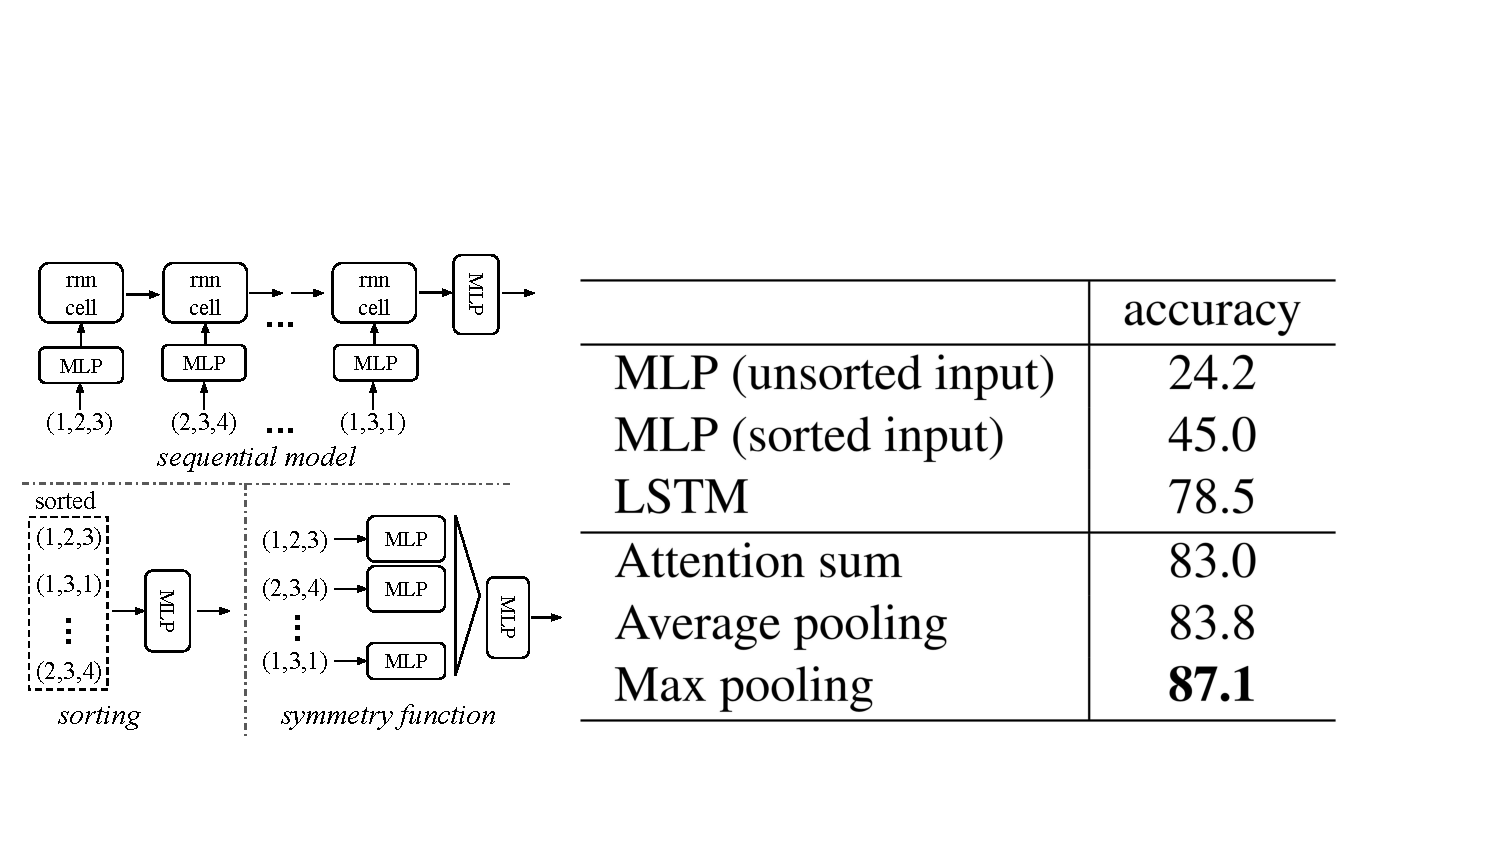
\includegraphics[width=\linewidth]{fig/order_invariant2.pdf}
    \caption{\textbf{三种实现顺序不变性的方法}神经元尺寸为64,64,64,128,1024,的5层隐藏层的多层感知机(MLP)应用在点集上,所有点共享一个简单的MLP副本。靠近输出的MLP共有两层,尺寸为512,256。}
    \label{fig:order_invariant}
\end{figure}

\paragraph{输入和特征转换的有效性} 在表~\ref{tab:transform}中,我们展示了我们的输入和特征转换(用于对齐)的积极影响。有趣的是,最基本的架构已经取得了相当合理的结果。使用输入转换可提高 $0.8\%$ 的性能。正则化损失是高维变换起作用所必需的。通过结合转换和正则化项,我们实现了最佳性能。

\begin{table}[b!]
    \small
    \centering
    \begin{tabular}[width=\linewidth]{l|c}
    \hline
    Transform              & accuracy \\ \hline
    none                   & 87.1     \\ \hline
    input (3x3)            & 87.9     \\
    feature (64x64)        & 86.9     \\
    feature (64x64) + reg. & 87.4     \\ \hline
    both                   & \textbf{89.2}     \\ \hline
    \end{tabular}
    \caption{\textbf{输入特征转换的效果} 评价指标是ModelNet40测试集上的总体分类准确率}
    \label{tab:transform}
\end{table}


% \paragraph{Effects of Max Layer Size and Number of Points} Here we show our model's performance change with regard to the size of the first max layer output as well as the number of input points. In Fig~\ref{fig:net_param} we see that performance grows as we increase the number of points however it saturates at around 1K points. The max layer size plays an important role, increasing the layer size from 64 to 1024 results in a $2-4\%$ performance gain. It indicates that we need enough point feature functions to cover the 3D space in order to discriminate different shapes.

% \begin{figure}
%     \centering
%     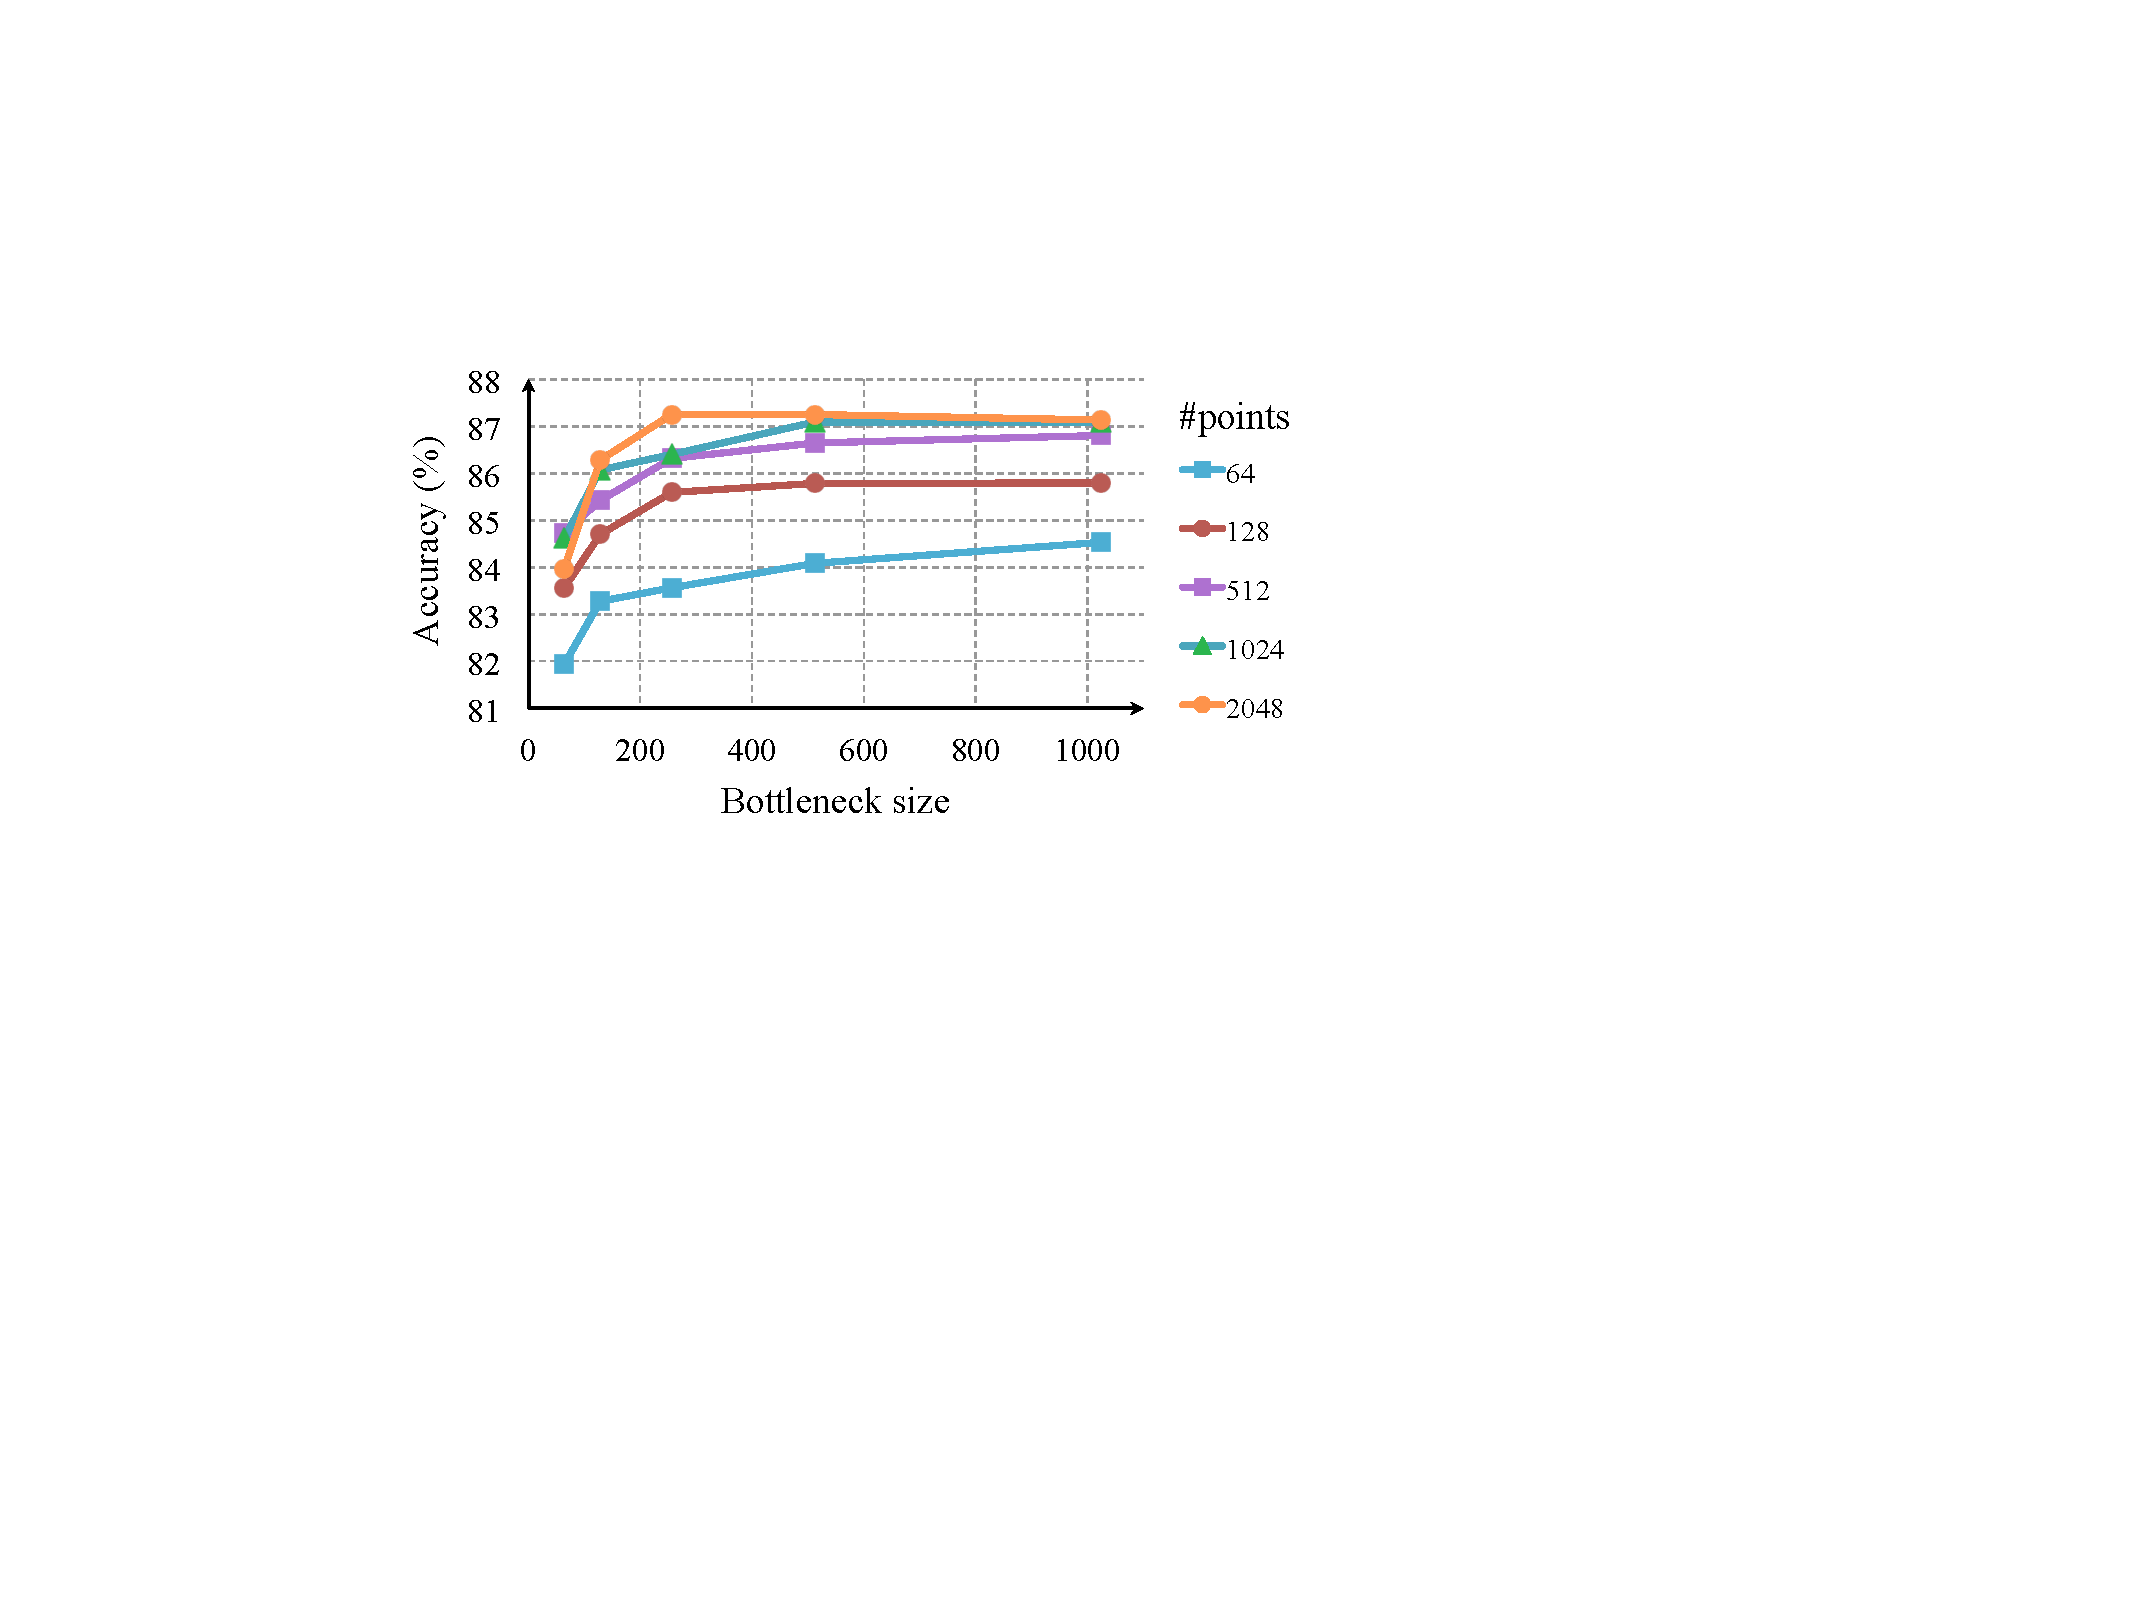
\includegraphics[width=0.8\linewidth]{fig/bottleneck.pdf}
%     \caption{\textbf{Effects of bottleneck size and number of input points.} The metric is overall classification accuracy on ModelNet40 test set.}
%     \label{fig:net_param}
% \end{figure}

\paragraph{鲁棒性测试} 我们展示了我们的PointNet不仅简单有效,还对各种输入损坏具有鲁棒性。我们使用与图~\ref{fig:order_invariant}的最大池化网络相同的架构。输入点被归一化为一个单位球体。结果如图~\ref{fig:robustness}。

A对于缺失点,当有 $50\%$ 的点缺失时,准确率仅下降 $2.4\%$ ,并且对于最远和随机输入采样则是 $3.8\%$ 。我们的网络在训练期间看到了异常点你,那么它对异常点也具有鲁棒性,。我们评估了两种模型:一种在具有 $(x,y,z)$ 坐标的点上进行训练;另一个在 $(x,y,z)$ 上加上点密度。即使当 $20\%$ 的点是异常值,网络也有超过 $80\%$ 的准确率。图~\ref{fig:robustness}右侧显示了网络对点扰动的鲁棒性。

\begin{figure}
    \centering
    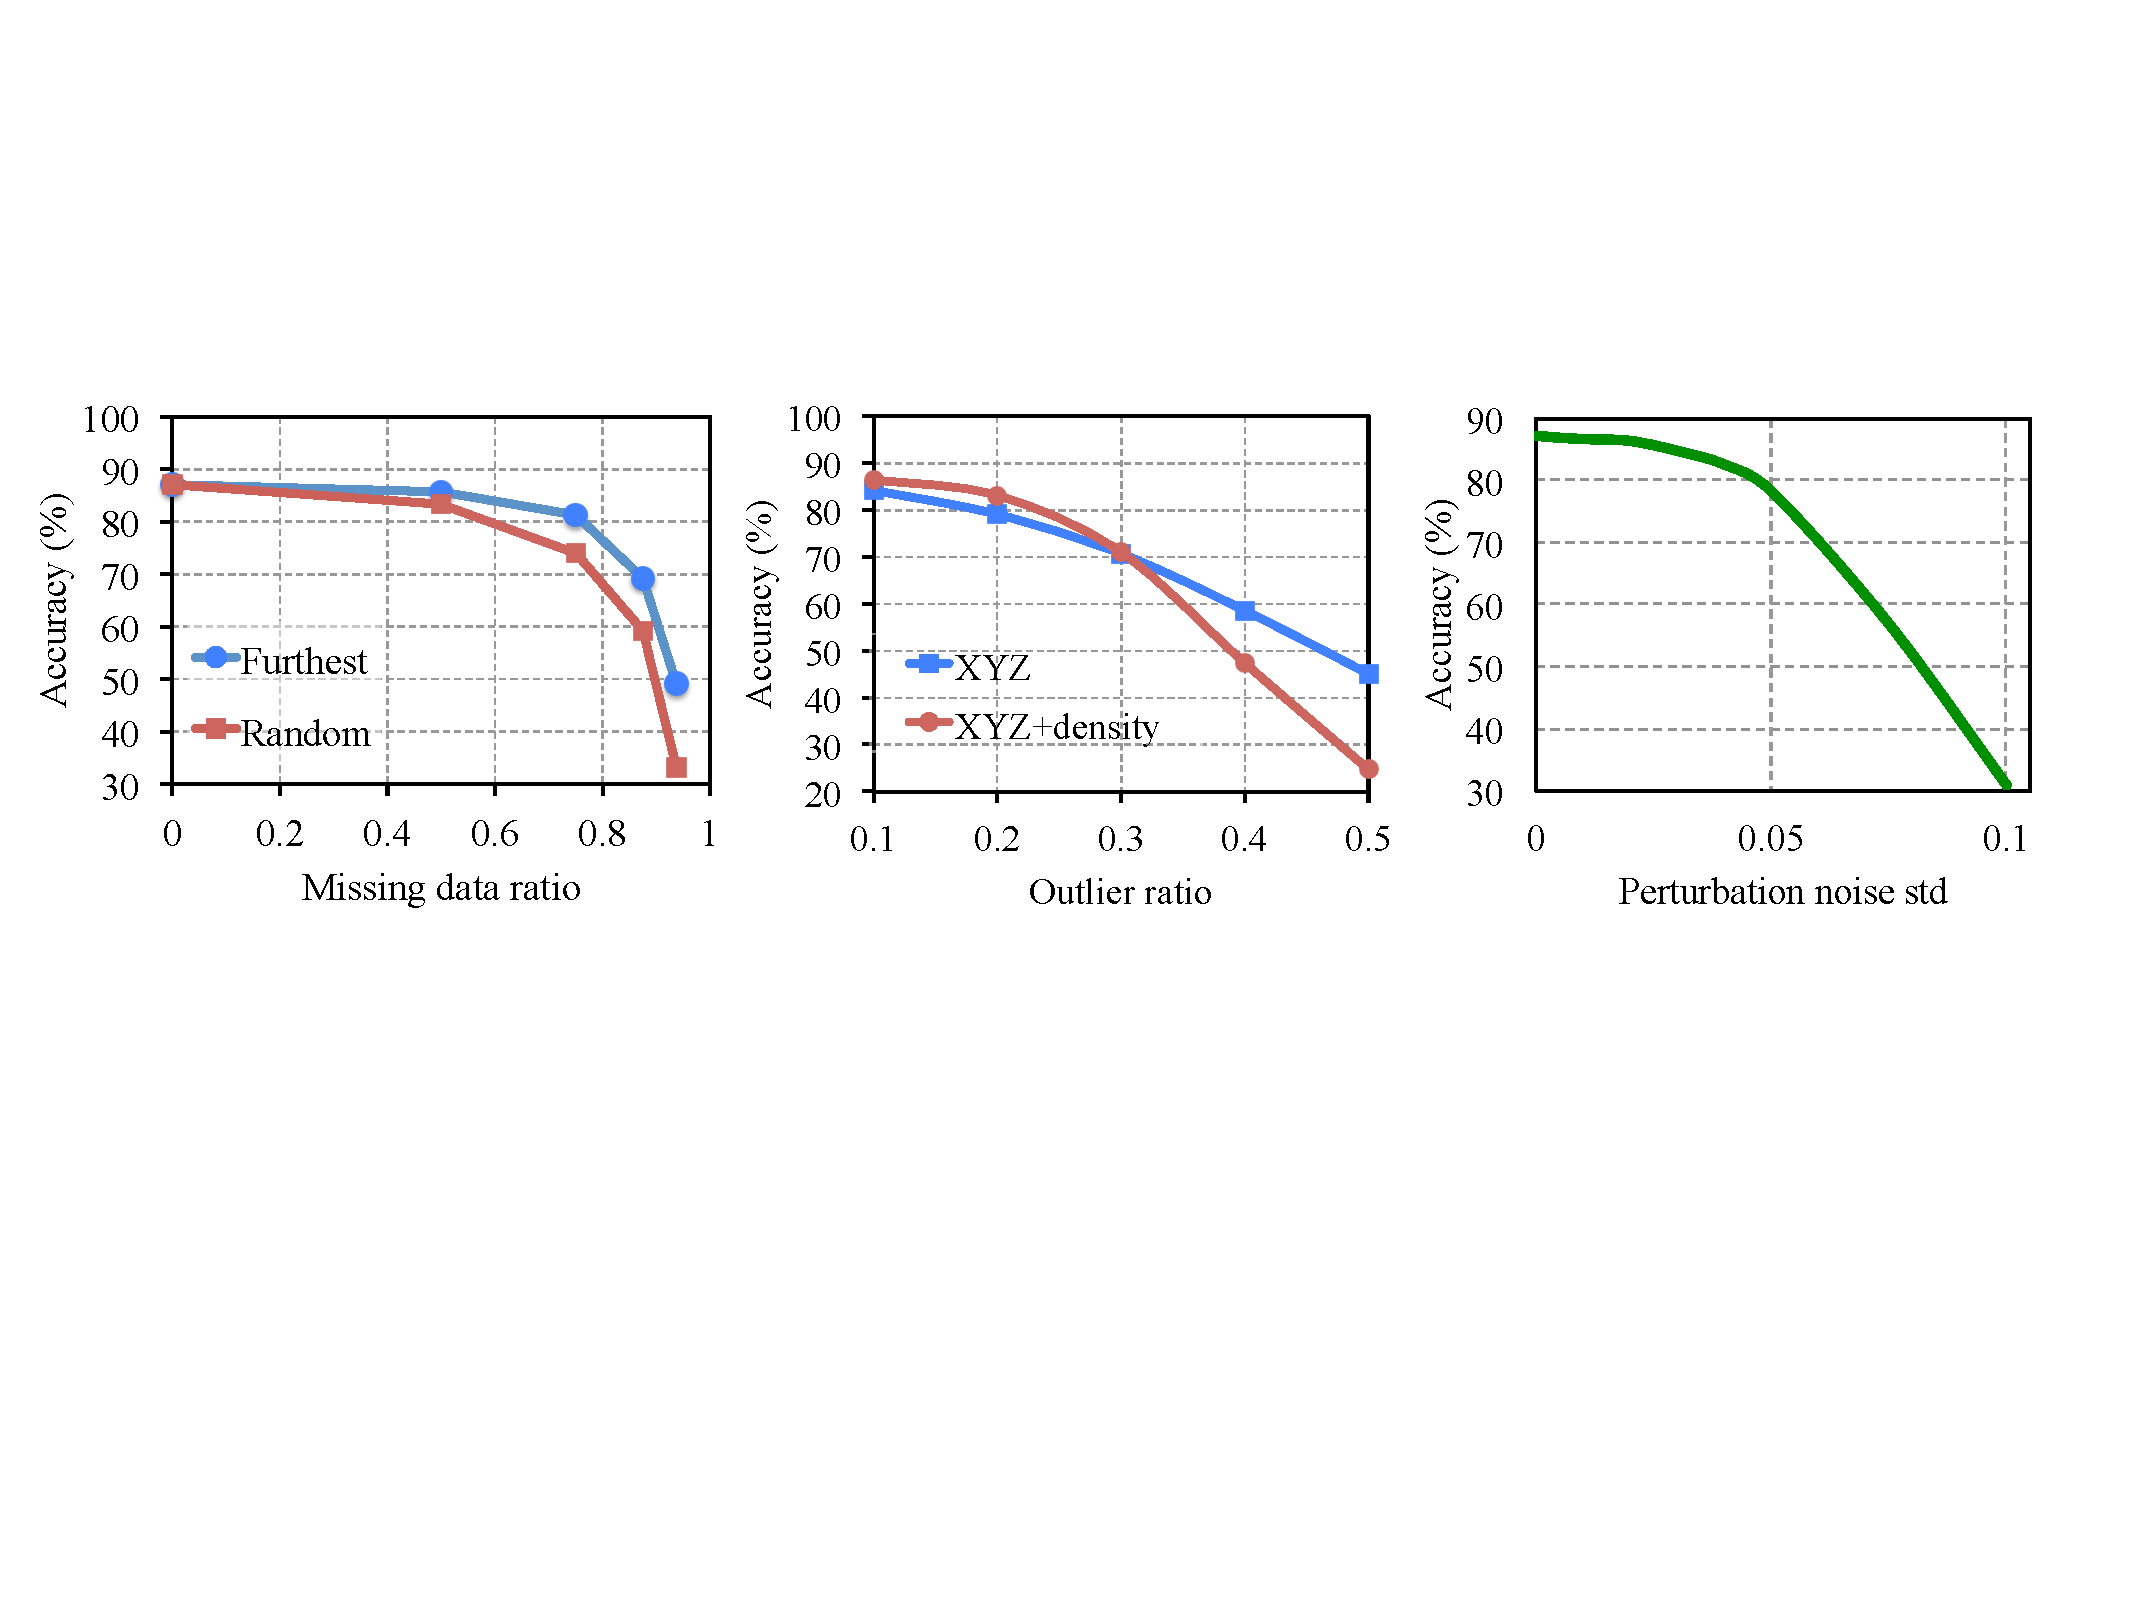
\includegraphics[width=\linewidth]{fig/robustness.pdf}
    \caption{\textbf{PointNet鲁棒性测试} 评价指标是ModelNet40测试集上的总体分类准确率。 左侧: 删除点的情况 Furthest意思是对1024个原始点采用最远点采样。 中间: 离群点插入的情况。离群点均匀的分布在单位球体中。 右侧: 点扰动的情况。单独对每个点进行高斯噪声扰动}
    \label{fig:robustness}
\end{figure}

\begin{comment}
\paragraph{MNIST Digit Classification} While we focus on 3D point cloud learning, a sanity check experiment is to apply our network on a 2D point clouds - pixel sets.

To convert an MNIST image into a 2D point set we threshold pixel values and add the pixel (represented as a point with XY coordinate in the image) with values larger than 128 to the set. We use a set size of 256. If there are more than 256 pixels int he set, we randomly subsample it; if there are less, we pad the set with the one of the pixels in the set (due to our max operation, which point used for the padding will not affect outcome). 
3
As seen in Table~\ref{tab:mnist}, we compare with a few baselines including multi-layer perceptron that considers input image as an ordered vector, a RNN that consider input as sequence from pixel (0,0) to pixel (27,27), and a vanila CNN. It's interesting to see that our model can achieve quite good performance by considering the image as a 2D point set.

% vanila CNN: https://www.microsoft.com/en-us/research/publication/best-practices-for-convolutional-neural-networks-applied-to-visual-document-analysis/
\begin{table}[h!]
    \centering
    \begin{tabular}[width=\linewidth]{l|c|c}
    \hline
    ~                      & input & error (\%) \\ \hline
    Multi-layer perceptron~\cite{simard2003best} & vector & 1.60  \\
    LeNet5~\cite{lecun1998gradient}                 & image & 0.80 \\ \hline
    Ours PointNet          & point set & 0.78 \\ \hline
    \end{tabular}
    \caption{\textbf{MNIST classification results.} We compare with vanila versions of other deep architectures to show that our network based on point sets input is achieving reasonable performance on this traditional task.}
    \label{tab:mnist}
\end{table}
\end{comment}


% \begin{figure}[b!]
%     \centering
%     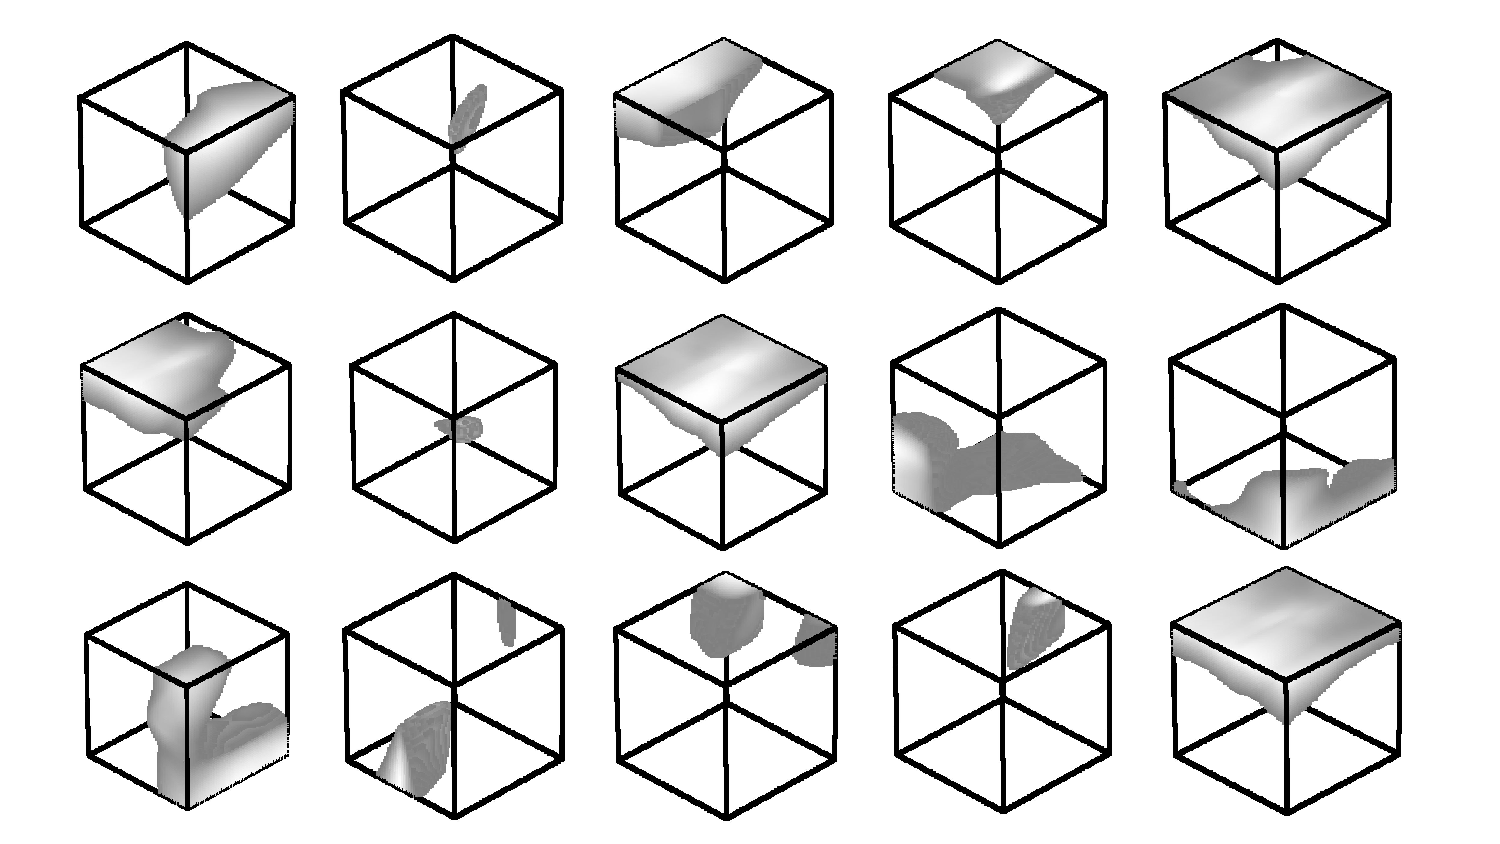
\includegraphics[width=0.7\linewidth]{fig/kernels.pdf}
%     \caption{\textbf{Point function visualization.} For each per-point function $h$, we calculate the values $h(p)$ for all the points $p$ in a cube of diameter two located at the origin, which spatially covers the unit sphere to which our input shapes are normalized when training our PointNet. In this figure, we visualize all the points $p$ that give $h(p)>0.5$ with function values color-coded by the brightness of the voxel. We randomly pick 15 point functions and visualize the activation regions for them.}
%     \label{fig:functions}
% \end{figure}


\subsection{可视化PointNet}
\label{sec:visualizing_pointnet}
% We design two experiments to visualize what has been learnt by the PointNet. The results are consistent with the theoretical analysis in Sec~\ref{sec:theory}. In the first experiment, we visualize the learnt point function $h(x)$ in Eq~\ref{eq:approx}, which demonstrates that our network learns a family of optimization criteria that selects informative points from the cloud. Our second experiment illustrates the robustness of our network, as explained in Thm~\ref{thm:thm2}.

% \paragraph{Point Function Visualization} As discussed in Sec~\ref{sec:pointnet_arch}, our network computes $K$ (we take $K=1024$ in this experiment) dimension point features for each point and aggregates all the per-point local features via a max pooling layer into a single $K$-dim vector, which forms the global shape descriptor. 

% To gain more insights on what the learnt per-point functions $h$'s detect, we visualize the points $p_i$'s that give high per-point function value $f(p_i)$ in Fig~\ref{fig:functions}. This visualization clearly shows that different point functions learn to detect for points in different regions with various shapes scattered in the whole space. 

\begin{comment}
This visualization is similar to the kernel visualization in convolutional neural networks in the sense that we'd like to know what input patterns would activate a specific neuron. However, our point function is behaving in a very differnt way from conv kernels.
\end{comment}

在图~\ref{fig:recon},我们可视化了一些样本形状 $S$ 的 \textit{关键点集} $\mathcal{C}_S$ 和 \textit{上边界形状} $\mathcal{N}_S$ (如Thm~\ref{thm:thm2}所述)。两个形状之间的点集将给出完全相同的全局形状特征 $f(S)$。

从图~\ref{fig:recon} 可以清楚地看出, \textit{关键点集} $\mathcal{C}_S$中对最大池化特征有贡献的点,总结了形状的主干。
%, or sample a sparse collection of points to describe the geometry of the whole shape.
\textit{上界形状} $\mathcal{N}_S$ 说明了与输入点云 $S$ 具有相同全局形状特征 $f(S)$ 的最大可能点云。$\mathcal{C}_S$ 和 $\mathcal{N}_S$反映了PointNet的鲁棒性,这意味着丢失一些非关键点不会改变全局形状特征 $f(S)$。



% We visualize the shape family, as discussed in Thm~\ref{thm:thm2}, including all the shapes between the \textit{critical point set} $\mathcal{C}_S$ and the \textit{upper-bound shape} $\mathcal{N}_S$ that gives the same global feature $f(S)$ with respect to a given shape $S$.

\begin{figure}[b]
    \centering
    % \includegraphics[width=0.8\linewidth]{fig/recon.pdf}
    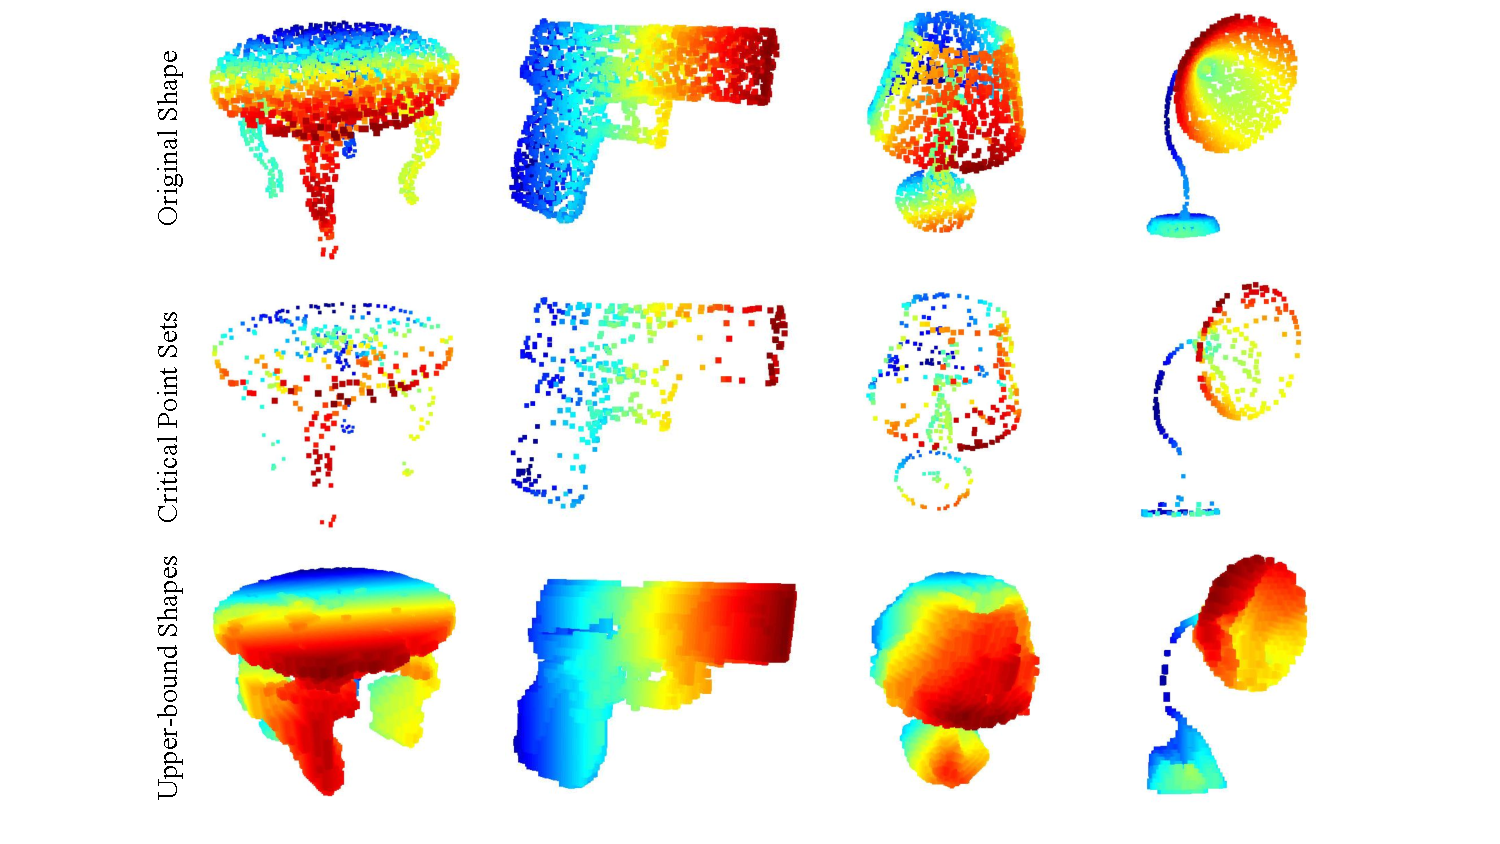
\includegraphics[width=0.8\linewidth]{fig/kp_ss_visu1.pdf}
    \caption{\textbf{关键点集和上界形状} 关键点集和上界形状共同决定了给定形状的全局形状特征,任何处于关键点集和上界形状间的点云都有同样一致的特征。 我们通过色彩编码来体现物体的深度信息。}
    \label{fig:recon}
\end{figure}

% Fig~\ref{fig:recon} shows the \textit{critical point sets} $\mathcal{C}_S$ and \textit{upper-bound shapes} $\mathcal{N}_S$ for four selected shapes. 
%The original input point clouds are rendered in the first row while the $\mathcal{C}_S$ and $\mathcal{N}_S$ for them are shown in the second and their rows respectively.
%The $\mathcal{C}_S$ for a given shape $S$ includes the points from the original point cloud that activates some point function $h_i$'s the most. 
$\mathcal{N}_S$ 是通过将边长为2的立方体中的所有点经过网络前向传播后,选择点函数值$(h_1(p), h_2(p), \cdots, h_K(p))$ 不大于全局形状描述符的点 $p$ 来构建的。
% It is not hard to see that all the shapes $S'$ that cover $\mathcal{C}_S$ and are contained by $\mathcal{N}_S$ give the exactly same global feature $f(S')=f(S)$. The transition shape family entails the robustness of the our PointNet, meaning that adding noisy jitterings or losing some non-critical points do not change the learnt shape signature and thus do not affect our classification or segmentation results.

\begin{comment}
We start from a max pooled vector of a specific input point cloud $X$, and find a set of point cloud $S$ (it's a set of point sets) where each point cloud in the set $S$ will result in the same max pooled vector as to $X$. In another word, we will reconstruct the input with only the knowledge of $X$ and the network parameters.

Assuming when feeding input point cloud $X$ to the network the first max-pooling layer's output is $g(X) = MAX\{f(x_1), f(x_2), ..., f(x_N)\} \in \R^{1024}$, where $X = \{x_1, x_2, ..., x_N\}$. We achieve the reconstruction by firstly construct a dense volumetric grids. Each voxel represents a point in 3D space. Then we will sweep through each point $p$ in the volume and judge whether this point's feature $f(p) \in \R^{1024}$ has any value larger than that in the corresponding dimension of $g(X)$. If there is , it means the point $p$ cannot be the input that results in $g(X)$, so we will exclude this point. After sweeping the volume, all the points left are possible to be part of the input set $X$. This set of points forms a upper bound of any possible input set that gets max pooling outcome of $g(X)$. Some reconstructed results of this upper bound is visualized in the second row of Fig~\ref{fig:recon}.

On the other hand, if we know the input set (set $X$) and the network, we can know which input points (subset $Y$ of $X$) are actually contributing to the final value of the max pooled vector. Excluding all the points in $X \\ Y$ will not affect the result. We call this contributing set of points the lower bound of the input, as visualized in the third row of Fig~\ref{fig:recon}. Any point sets that fall between the lower bound and upper bound will result in exactly the same result.
\end{comment}





\subsection{时间和空间复杂度分析}
\label{sec:complexity}
表~\ref{pointnet_complexity} 总结了我们PointNet分类网络的空间(网络中的参数个数)和时间(浮点运算/样本)复杂性。我们还将PointNet与之前工作中的一组具有代表性的基于体积和多视图的架构进行了比较。

尽管MVCNN~\cite{su15mvcnn} 和Subvolume (3D CNN) ~\cite{qi2016volumetric} 实现了高性能,PointNet的计算成本更低,效率更高(以FLOPs/样本衡量:效率分别提高\emph{141倍} 和 \emph{8倍})。此外,就网络中的\#param(参数少\emph{17倍})而言,PointNet的空间效率比MVCNN高得多。此外,PointNet更具可扩展性——它的空间和时间复杂度为 $O(N)$ —— 与输入点的数量呈\emph{线性} 关系。然而,由于卷积占用计算时间,多视图方法的时间复杂度随图像分辨率\emph{平方级}增长,基于体积卷积的方法随着体积大小成\emph{立方级}增长。

根据经验,PointNet能够处理超过每秒100万个点用于点云分类(约1K对象/秒)或语义分割(约2个房间/秒),在TensorFlow上使用1080XGPU,显示出实时应用的巨大潜力。

\begin{table}[h!]
    \centering
    \begin{tabular}{|l|l|l|l|}
    \hline
    ~                & \#params & FLOPs/sample\\ \hline
    PointNet (vanilla)  & 0.8M                        & 148M \\
    PointNet         & 3.5M                         & 440M \\ \hline
    %VoxNet~\cite{maturana2015voxnet}           & 0.07M                        & 204M \\
    Subvolume~\cite{qi2016volumetric} & 16.6M                        & 3633M \\ \hline
    MVCNN~\cite{su15mvcnn}   & 60.0M                          & 62057M \\ \hline
    \end{tabular}
    \caption{\textbf{处理3D数据分类的深度学习架构的时间和空间复杂度} PointNet (vanilla) 是分类版的PointNet除去输入和特征转化部分的版本。 FLOP代表浮点运算操作。
    ``M'' 代表百万。 Subvolume和MVCNN都使用了多次旋转和多个视角池化后的数据,没有这些操作他们的表现会大大下降}
    \label{pointnet_complexity}
    \vspace{-3mm}
\end{table}

\section{结论}
\label{sec:conclusion}
在这项工作中,我们提出了一种新颖的、可以直接使用点云输入的深度神经网络 \emph{PointNet} 。我们的网络为许多3D识别任务提供了统一的方法,这些3D识别任务包括目标分类、零件分割和语义分割,同时在标准基准上获得与现有技术相当或更好的结果。我们还提供理论分析和可视化来理解我们的网络。



\mypara{致谢} 作者非常感谢三星GRO授予的资助、ONR MURI N00014-13-1-0341的资助、NSF授予资助IIS-1528025、Google重点研究奖、来自Adobe公司的礼物和NVIDIA的硬件捐赠的支持。

{\small

\begin{thebibliography}{}
\documentclass[10pt,twocolumn,letterpaper,UTF8]{article}
\hyphenpenalty=2000
\textwidth=6.5in
\textheight=9.0in
\evensidemargin=0.0in
\oddsidemargin=0.0in
\topmargin=-0.5in
\clubpenalty=4000
\widowpenalty=4000
\displaywidowpenalty=500

\newlength\minalignvsep

\usepackage{cvpr}
\usepackage{times}
\usepackage{epsfig}
\usepackage{graphicx}
\usepackage{amsmath,amssymb,amsthm}
\usepackage{pbox}
\usepackage{epstopdf}
\usepackage{subfigure}
\usepackage{xspace}
\usepackage{comment}
\usepackage{lipsum}
%\usepackage{jeffe}
\usepackage{enumitem}

% 中文支持
\usepackage{ctex}
\usepackage[T1]{fontenc}
\usepackage{mathpazo}
\usepackage{fontspec}
\setmainfont[Scale = 1]{TeX Gyre Pagella}
\setCJKmainfont[ItalicFont=Noto Serif CJK SC Bold, BoldFont=Noto Serif CJK SC Black, Scale = 1]{Noto Serif CJK SC}

\newcommand{\cmt}[2]{[#1: #2]}
\newcommand{\todo}[1]{\cmt{{\bf TODO}}{{\bf \color{red} #1}}}
\newcommand{\hao}[1]{\cmt{{\bf Hao}}{{\bf \color{red} #1}}}
\newcommand{\rqi}[1]{\cmt{{\bf Charles}}{{\bf \color{blue} #1}}}
\newcommand{\km}[1]{\cmt{{\bf Kaichun}}{{\bf \color{green} #1}}}
\newcommand{\leo}[1]{\cmt{{\bf Leo}}{{\bf \color{cyan} #1}}}

\newcommand{\shape}{S}
\newcommand{\image}{I}
\newcommand{\network}{\mathbb{G}}
\newcommand{\prob}{\mathcal{P}}

\newcommand{\para}[1]{\noindent{\bf #1}}

\newcommand{\softpara}{\paragraph}
\newcommand{\mypara}{\vspace*{-15pt}\paragraph}

\newcommand{\bmemo}[1]{\noindent{\color{blue}{\sf [[#1]]}}}

\newcommand{\denselist}{\itemsep 0pt\parsep=0pt\partopsep 0pt\vspace{-2pt}}
\newcommand{\bitem}{\begin{itemize}\denselist}
\newcommand{\eitem}{\end{itemize}}
\newcommand{\benum}{\begin{enumerate}\denselist}
\newcommand{\eenum}{\end{enumerate}}
\newcommand{\bdescr}{\begin{description}\denselist}
\newcommand{\edescr}{\end{description}}

\newcommand{\Remark}[1]     {{\sf [#1]}}

\setlength{\abovedisplayskip}{0pt}
\setlength{\belowdisplayskip}{0pt}

\newtheorem{theorem}{Theorem}

\newcommand{\myvec}[1]{\mathbf #1}
\newcommand\blfootnote[1]{%
  \begingroup
  \renewcommand\thefootnote{}\footnote{#1}%
  \addtocounter{footnote}{-1}%
  \endgroup
}
\newtheorem{innercustomthm}{Theorem}
\newenvironment{customthm}[1]
  {\renewcommand\theinnercustomthm{#1}\innercustomthm}
  {\endinnercustomthm}
  
% Include other packages here, before hyperref.

% If you comment hyperref and then uncomment it, you should delete
% egpaper.aux before re-running latex.  (Or just hit 'q' on the first latex
% run, let it finish, and you should be clear).
\usepackage[pagebackref=true,breaklinks=true,letterpaper=true,colorlinks,bookmarks=false]{hyperref}

\cvprfinalcopy % *** Uncomment this line for the final submission

\def\cvprPaperID{201} % *** Enter the CVPR Paper ID here
\def\httilde{\mbox{\tt\raisebox{-.5ex}{\symbol{126}}}}

% Pages are numbered in submission mode, and unnumbered in camera-ready
\ifcvprfinal\pagestyle{empty}\fi
\begin{document}

%%%%%%%%% TITLE
\title{PointNet: 针对三维分类点云分类与分割的深度学习模型
% PointNet: Deep Learning on Point Sets for 3D Classification and Segmentation
}

% \author{First Author\\
% Institution1\\
% Institution1 address\\
% {\tt\small firstauthor@i1.org}
% % For a paper whose authors are all at the same institution,
% % omit the following lines up until the closing ``}''.
% % Additional authors and addresses can be added with ``\and'',
% % just like the second author.
% % To save space, use either the email address or home page, not both
% \and
% Second Author\\
% Institution2\\
% First line of institution2 address\\
% {\tt\small secondauthor@i2.org}
% }

\author{Charles R. Qi*\qquad Hao Su* \qquad Kaichun Mo \qquad Leonidas J. Guibas\\Stanford University\\翻译: 浙江大学软件学院 2021 年夏令营 CAD 第三小组}

\maketitle
%\thispagestyle{empty}

%%%%%%%%% ABSTRACT
\begin{abstract}
{\normalfont
  \input{./tex/abstract}
}
\end{abstract}

%%%%%%%%% BODY TEXT
\section{引入}
\blfootnote{* 表示同等贡献。}
\input{./tex/intro}

\section{相关工作}
\input{./tex/related}

\section{问题陈述}
\input{./tex/problem}

\section{点集上的深度学习}
\input{./tex/arch}

\section{实验}
\input{./tex/exp}

\section{结论}
\input{./tex/conclusion}

\input{./tex/acknowledgement}

{\small

\begin{thebibliography}{}
\input{./pcl_review.bbl}
\end{thebibliography}

\bibliographystyle{ieee}
\bibliography{pcl}
}

\newpage

\input{./tex/supplementary}

% \newpage
% \section{Appendix}
% \input{./tex/appendix}

\end{document}

\end{thebibliography}

\bibliographystyle{ieee}
\bibliography{pcl}
}

\newpage

\appendix
\section*{附录}

\section{Overview}
% \begin{itemize}
%     \item \todo{Experiment.} compare pointnet with volumetric cnn and multi-view cnn on corrupted data (missing data). On both classification and segmentation. 
%     \item \todo{Writing.} network details.
%     \item \todo{Dump results.} more applications: normal prediction, correspondence, CAD model retrieval
%     \item (DONE) analysis on bottleneck and number of input points
%     \item (DONE) MNIST
%     \item \todo{Writing. Experiment.} details on object detection system
%     \item \todo{Dump results.} more output visualizations for critical points!! visualization of classification and part segmentation errors. visualization of detection results.
%     \item (DONE) proof of theorems
% \end{itemize}
该文件为主要论文提供了额外的定量结果,技术细节和更多定性的测试示例。 

在 Sec~\ref{sec:cla_robust}中,我们扩展了健壮性测试,以比较不完整输入下的PointNet和VoxNet。 在 Sec~\ref{sec:network}中我们提供了更多有关神经网络架构和训练参数的详细信息, 在 Sec~\ref{sec:detection}中我们描述了场景中的检测流程。Sec~\ref{sec:supp_application} 显示了PointNet的更多应用, 而 Sec~\ref{sec:architecture} 显示了更多的分析实验。 Sec~\ref{sec:proof} 为我们在PointNet上的理论提供了证明。 最后,我们在 Sec~\ref{sec:visu}中显示了更多的可视化结果。


\section{PointNet和VoxNet的比较 (Sec 5.2)}
\label{sec:cla_robust}
我们扩展了第 5.2 节鲁棒性测试中的实验,以比较PointNet和VoxNet~\cite{maturana2015voxnet}(一个用于体积表示的代表性结构)对输入点云中缺失数据的鲁棒性。两个网络都在以 1024 个点作为输入的相同训练测试集上进行训练。对于VoxNet,我们将点云体素化为 $32 \times 32 \times 32$ 的网格,并通过绕上轴随机旋转和抖动来增加训练数据。

在测试时,输入点按一定比例随机丢弃。由于VoxNet对旋转很敏感,它的预测使用来自点云的 12 个视点的平均分数。如图~\ref{fig:compare}所示,我们的PointNet对缺失点更加鲁棒。 当一半的输入点丢失时,VoxNet 的准确率急剧下降,从 $86.3\%$ 到 $46.0\%$,相差 $40.3\%$,而我们的 PointNet 的性能下降只有 $3.7\%$。这可以通过我们 PointNet 的理论分析和解释来解释——它正在学习使用 \textit{critical points} 的集合来总结形状,因此它对缺失数据非常健壮。


\begin{figure}[h!]
    \centering
    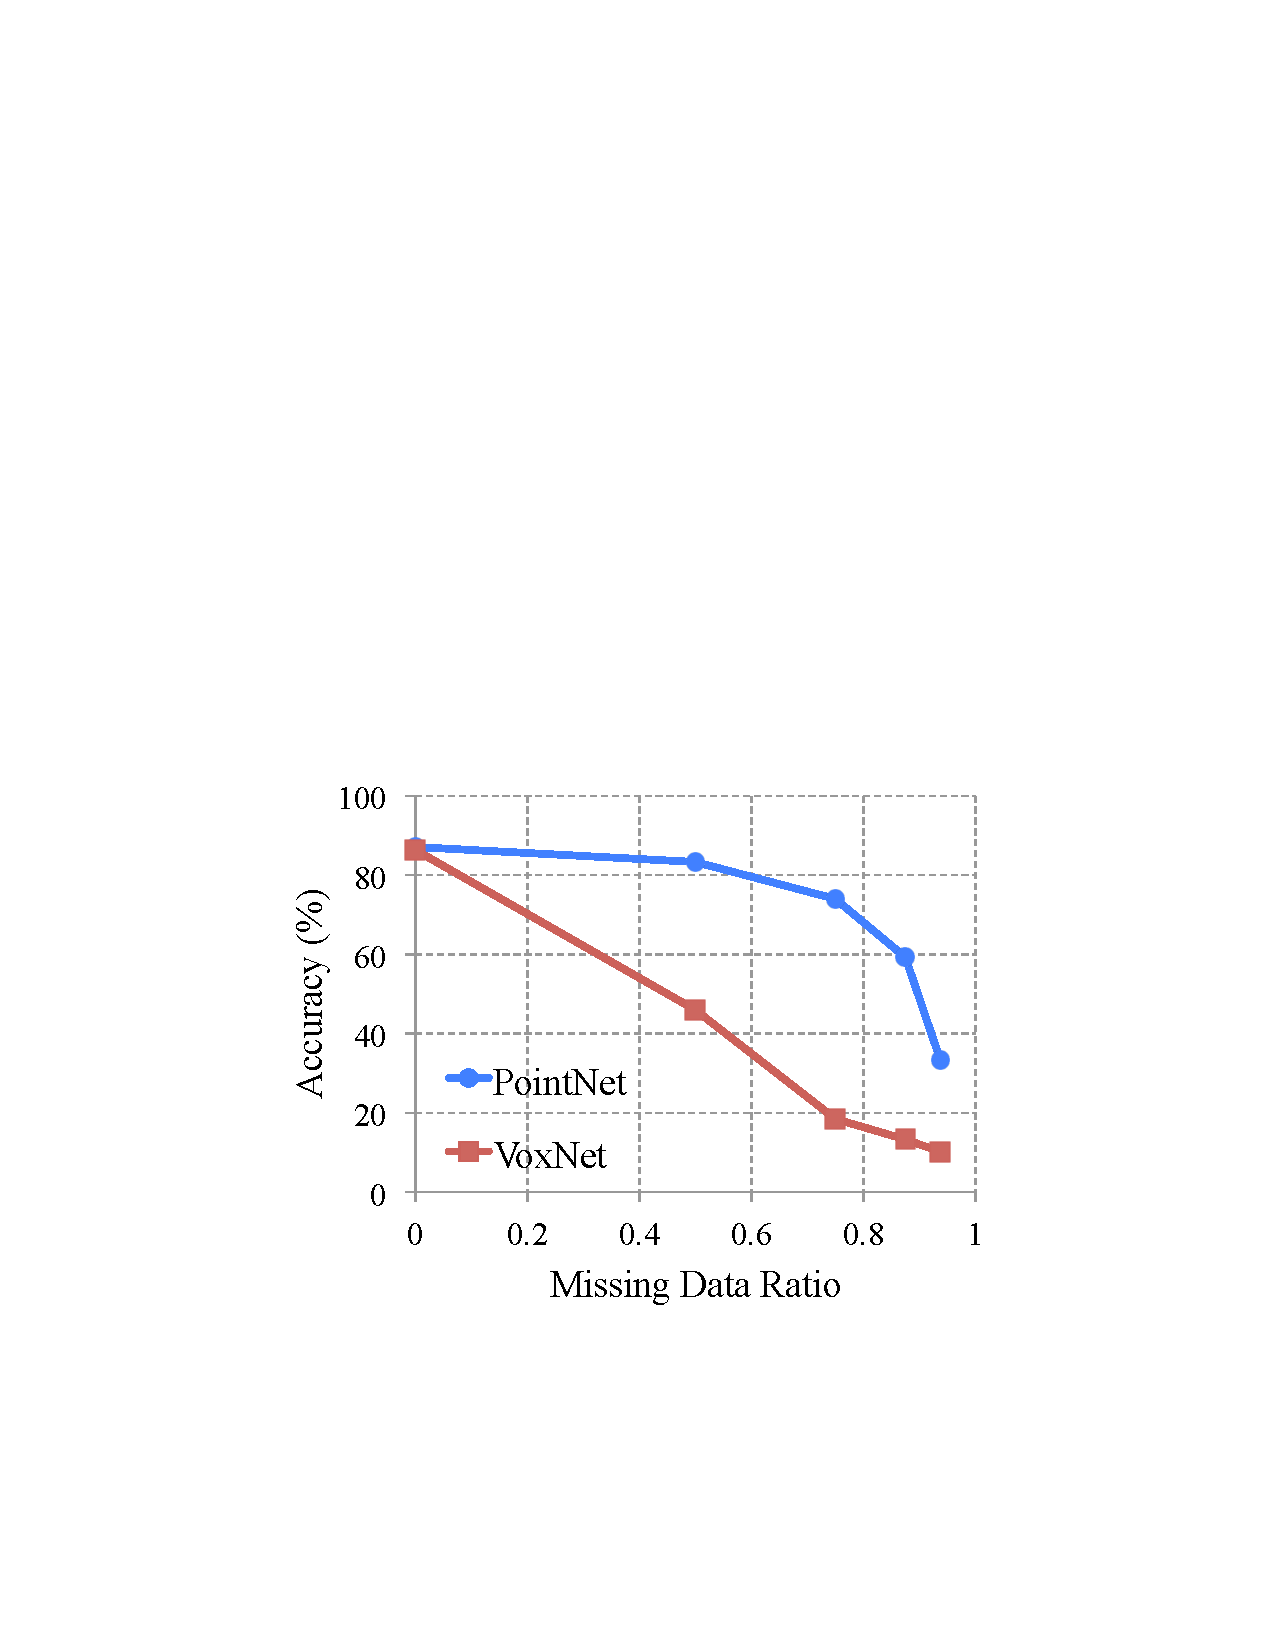
\includegraphics[width=0.7\linewidth]{fig/pointnet_vs_voxnet.pdf}
    \caption{\textbf{在不完整输入数据下的PointNet v.s. VoxNet~\cite{maturana2015voxnet} } 指标是 ModelNet40 测试集上的整体分类准确率。请注意,VoxNet 使用 12 个视点平均,而 PointNet 仅使用点云的一个视图。显然 PointNet 对缺失点具有更强的鲁棒性。}
    \label{fig:compare}
\end{figure}

% =============================
% Network details
% =============================
\section{网络架构和训练细节 (Sec 5.1)}
\label{sec:network}
\paragraph{PointNet分类网络}由于论文正文中已经说明了基本的体系结构,因此我们在此处提供有关联合对齐/变换网络和训练参数的更多详细信息。

第一个转换网络是一个mini-PointNet,它直接以未处理的点云为输入,并回归成一个$3\times3$的矩阵。这个网络由一个每个点共享的 $MLP(64,128,1024)$ 网络(输出尺寸分别为64, 128, 1024), 一个点间max pooling和两个全连接层(输出尺寸分别为$512$, $256$)组成。输出矩阵初始值为单位矩阵。除了最后一层,其余所有层都应用了ReLU和Batch Normalization。 第二个变换网络与第一个结构相同,除了输出矩阵尺寸为$64\times64$。输出矩阵也被初始化为单位阵。将正则化损失(权重为0.001)添加到softmax分类损失中,以使矩阵接近正交。

训练时,在估计类别概率前,对最后一层全连接层(维度$256$)应用了keep ratio 为$0.7$的dropout。
Batch Normalization的衰减率从初始的$0.5$逐渐增加到$0.99$。使用adam优化器,初始学习率设置为$0.001$,momentum为$0.9$,batch size为$32$。学习率每迭代20次下降一半。在TensorFlow下用GTX1080 GPU和ModelNet数据集训练,网络需要3-6个小时收敛。

\paragraph{PointNet分割网络}分割网络是PointNet分类网络的一个延伸。对于每个点,将局部点特征(第二个转换网络之后的输出)和全局特征(max pooling的输出)连接在一起。 在分割网络中不使用dropout。训练参数与分类网络相同。

关于形状零件分割的任务,我们对基本分割网络体系结构进行了一些修改 (正文中的图2) 以实现最佳性能。如图~\ref{fig:part_seg_net}所示。 我们添加了一个one-hot向量来显示输入类别并与max pooling的输出连接。 我们还在某些层中增加了神经元个数,并添加了skip links以收集不同层中的局部点特征,并将它们连接起来以形成点特征输入到分割网络中。

\begin{figure}
\centering
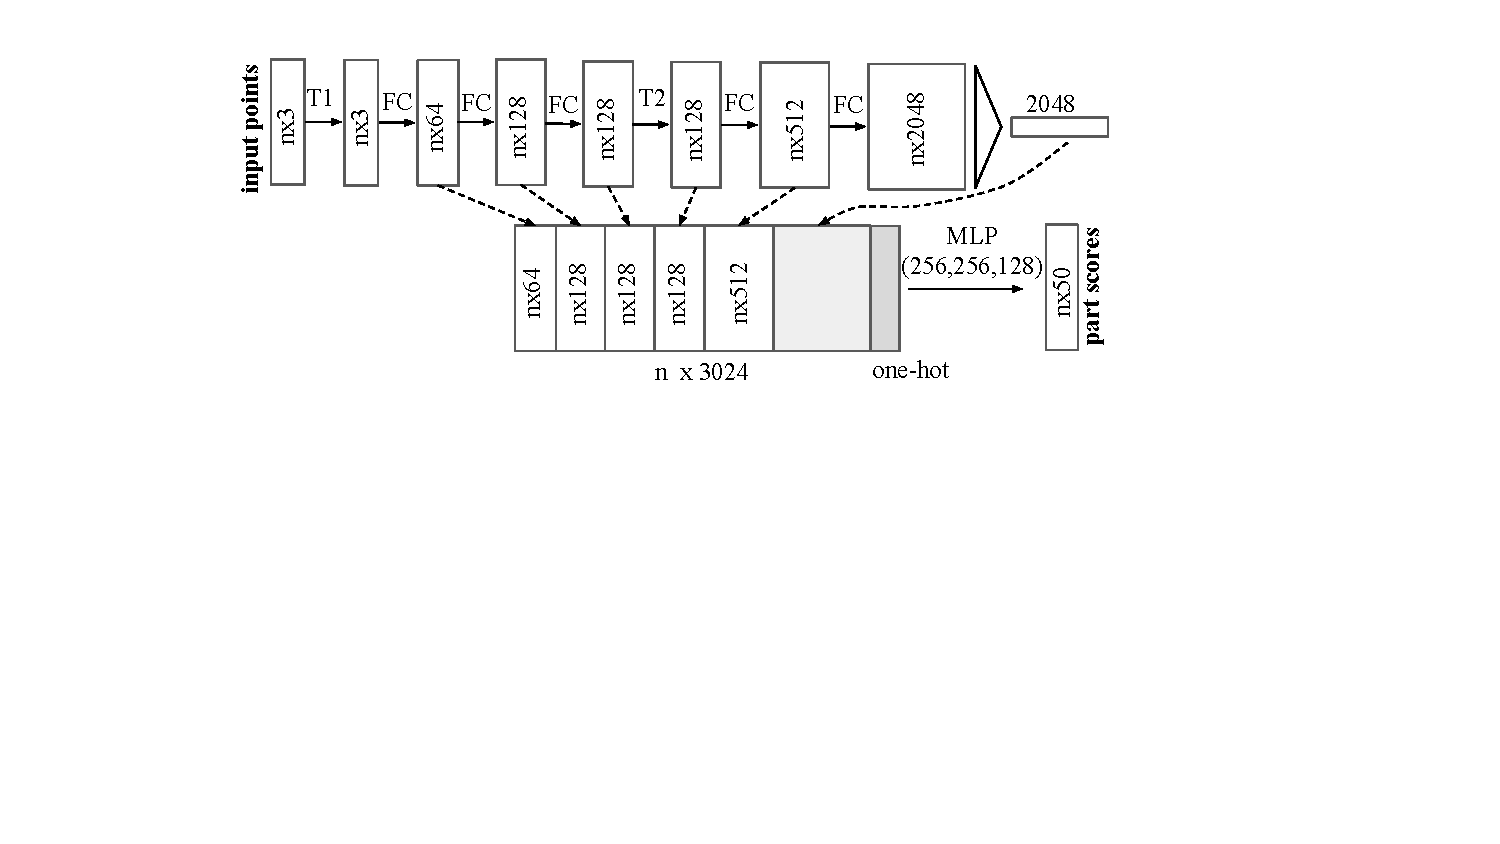
\includegraphics[width=\linewidth]{fig/part_seg_net.pdf}
\caption{\textbf{零件分割的网络架构} T1和T2是输入点和特征的对齐/变换网络。FC是在每个点上操作的全连接层。MLP是每一点上的多层感知器。One-hot是一个大小为16的向量,表示输入形状的类别。}
\label{fig:part_seg_net}
\end{figure}

尽管 \cite{Wu2014248} 和 \cite{Yi16} ]独立地处理每个对象类别, 但由于缺少某些类别的训练数据 (第一行显示了数据集中所有类别的形状总数), 我们训练了跨类别的PointNet(但是使用one-hot向量来指示类别).为了进行公平比较,在测试这两个模型时,我们只预测给定特定对象类别的部分标签。

对于语义学分割任务,应用的是与论文主体中相同的基本网络结构,如图2。

使用ShapeNet part 数据集训练需要大约6-12小时,使用Stanford semantic parsing数据集训练大概需要半天。

\paragraph{基准3D CNN分割网络}
在ShapeNet零件分割实验中,我们将建议的分割版本PointNet与两种传统方法以及3D体积CNN网络基准进行了比较。 在图~\ref{fig:voxnet}中, 我们展示了我们使用的基准3D体积CNN网络。 我们将众所周知的3D CNN架构,例如VoxNet \cite{maturana2015voxnet} 和 3DShapeNets \cite{wu20153d} 推广到完全卷积的3D CNN分割网络。

%In the CAD model part segmentation experiment, we compare our proposed segmentation version PointNet to two traditional methods based on shape local features and inter-shape correspondence, as well as a 3D volumetric CNN network as baseline methods. Our PointNet method is a data-driven deep learning method. The comparison between traditional methods to data-driven methods are inherently hard since data-driven methods require more training data than traditional methods. Though we try to test all the methods on the same ShapeNet train/validation/test split, we still think it is crucial to compare our proposed learning-based PointNet with another deep learning method. In Fig.~\ref{fig:voxnet}, we show the baseline 3D volumetric CNN network we use. We generalize the well-known 3D CNN architectures, such as VoxNet \cite{maturana2015voxnet} and 3D ShapeNet \cite{wu20153d} that are invented for classification task, to a 3D CNN segmentation network.

\begin{figure}[t!]
\centering
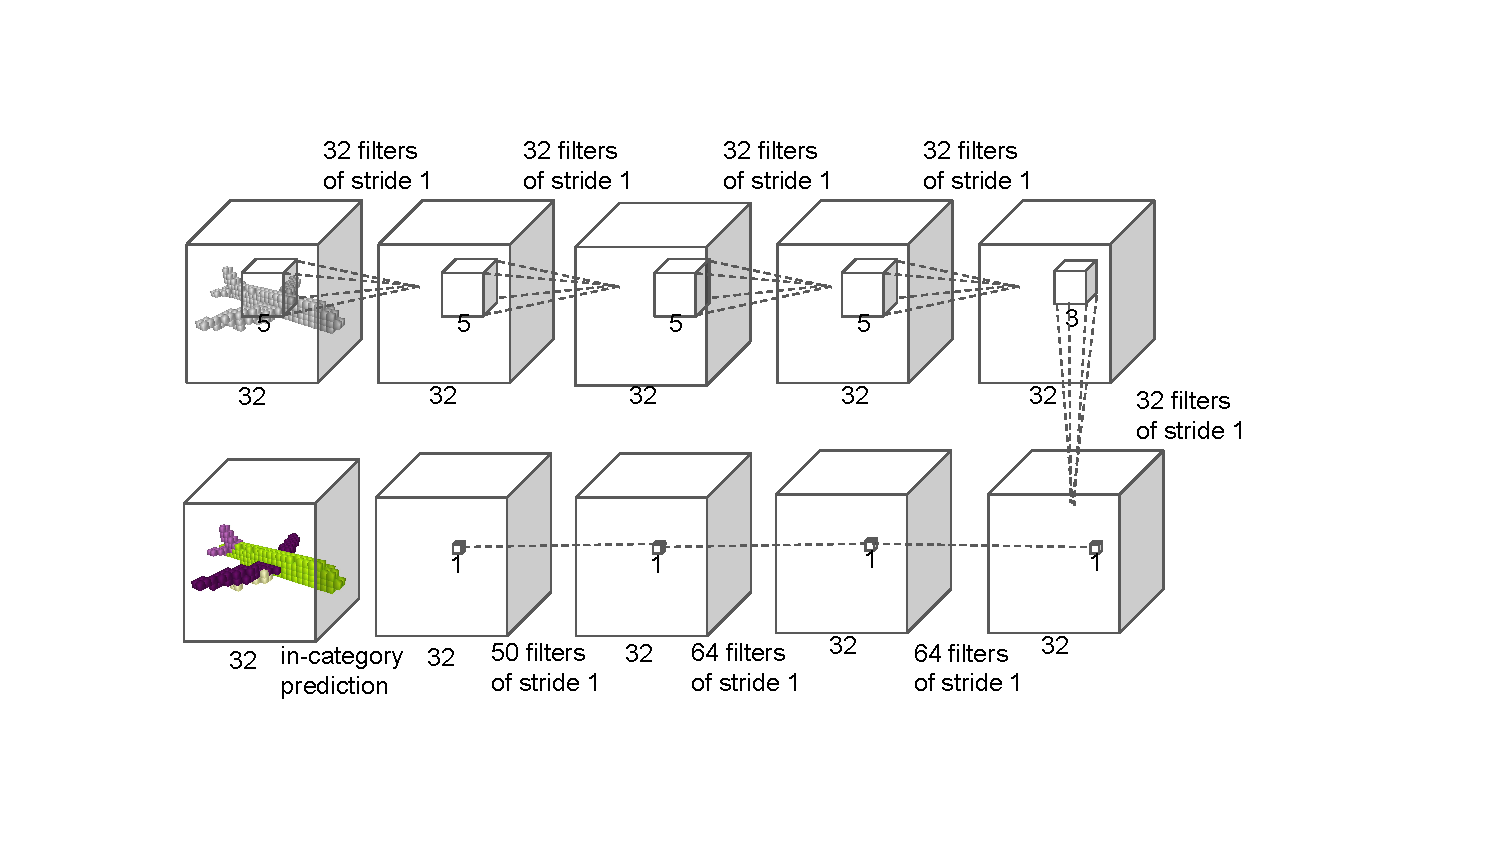
\includegraphics[width=\linewidth]{fig/voxnet.pdf}
\caption{\textbf{基准3D CNN分割网络.} 该网络是完全卷积化的,并且可以预测每个体素的部分分数}
\label{fig:voxnet}
\end{figure}
对于给定的点云,我们首先将其转换为具有$32 \times 32 \times 32$分辨率的占用网格的体积表示形式。然后,依次使用五个具有32个输出通道和步长为1的3D卷积核来提取特征。每个体素的感受野为19。 %In order to do the final per-pixel label prediction, we choose to keep the size of the feature maps to $32 \times 32 \times 32$ by allowing zero-padding. Zero-padding is reasonable since there are no occupancy for those padded voxels.
最后,将大小为$1\times 1\times 1$的3D卷积序列附加到计算出的特征图上,以预测每个体素的分割标签。除最后一层外,所有层均使用ReLU和Batch Normalization。该网络是跨类别训练的,但是,为了与给出对象类别的其他基准方法进行比较,我们仅考虑给定对象类别中的输出得分。

\section{Details on Detection Pipeline (Sec 5.1)}
\label{sec:detection}
我们基于语义分割结果和我们的对象分类 PointNet 构建了一个简单的 3D 对象检测系统。

我们使用带有分割分数的连接组件来获取场景中的对象提议。从场景中的一个随机点开始,我们找到它的预测标签,并使用 BFS 搜索附近具有相同标签的点,搜索半径为 $0.2$ 米。如果结果集群有超过 200 个点(假设 1m x 1m 区域中有 4096 个点样本),则集群的边界框被标记为一个对象提议。对于每个提议的对象,它的检测分数计算为该类别的平均点分数。在评估之前,面积/体积极小的提案被裁剪。对于桌子、椅子和沙发,边界框会延伸到地板,以防腿与座椅/表面分开。

我们观察到,在某些房间(例如礼堂)中,许多物体(例如椅子)彼此靠近,其中连接的组件无法正确地分割出单个的物体。因此,我们利用我们的分类网络并使用滑动形状方法来缓解椅子类的问题。我们为每个类别训练一个二元分类网络,并使用分类器进行滑动窗口检测。结果框通过非最大抑制进行裁剪。将来自连接组件和滑动形状的建议框组合起来进行最终评估。

在 图~\ref{fig:pr_curve} 中,我们展示了目标检测的准确率-召回率曲线。 我们训练了六个模型,其中每个模型都在五个区域进行训练并在左侧区域进行测试。在测试阶段,每个模型都在它从未见过的区域进行测试。将所有六个区域的测试结果汇总以生成 PR 曲线。
 
 \begin{figure}
 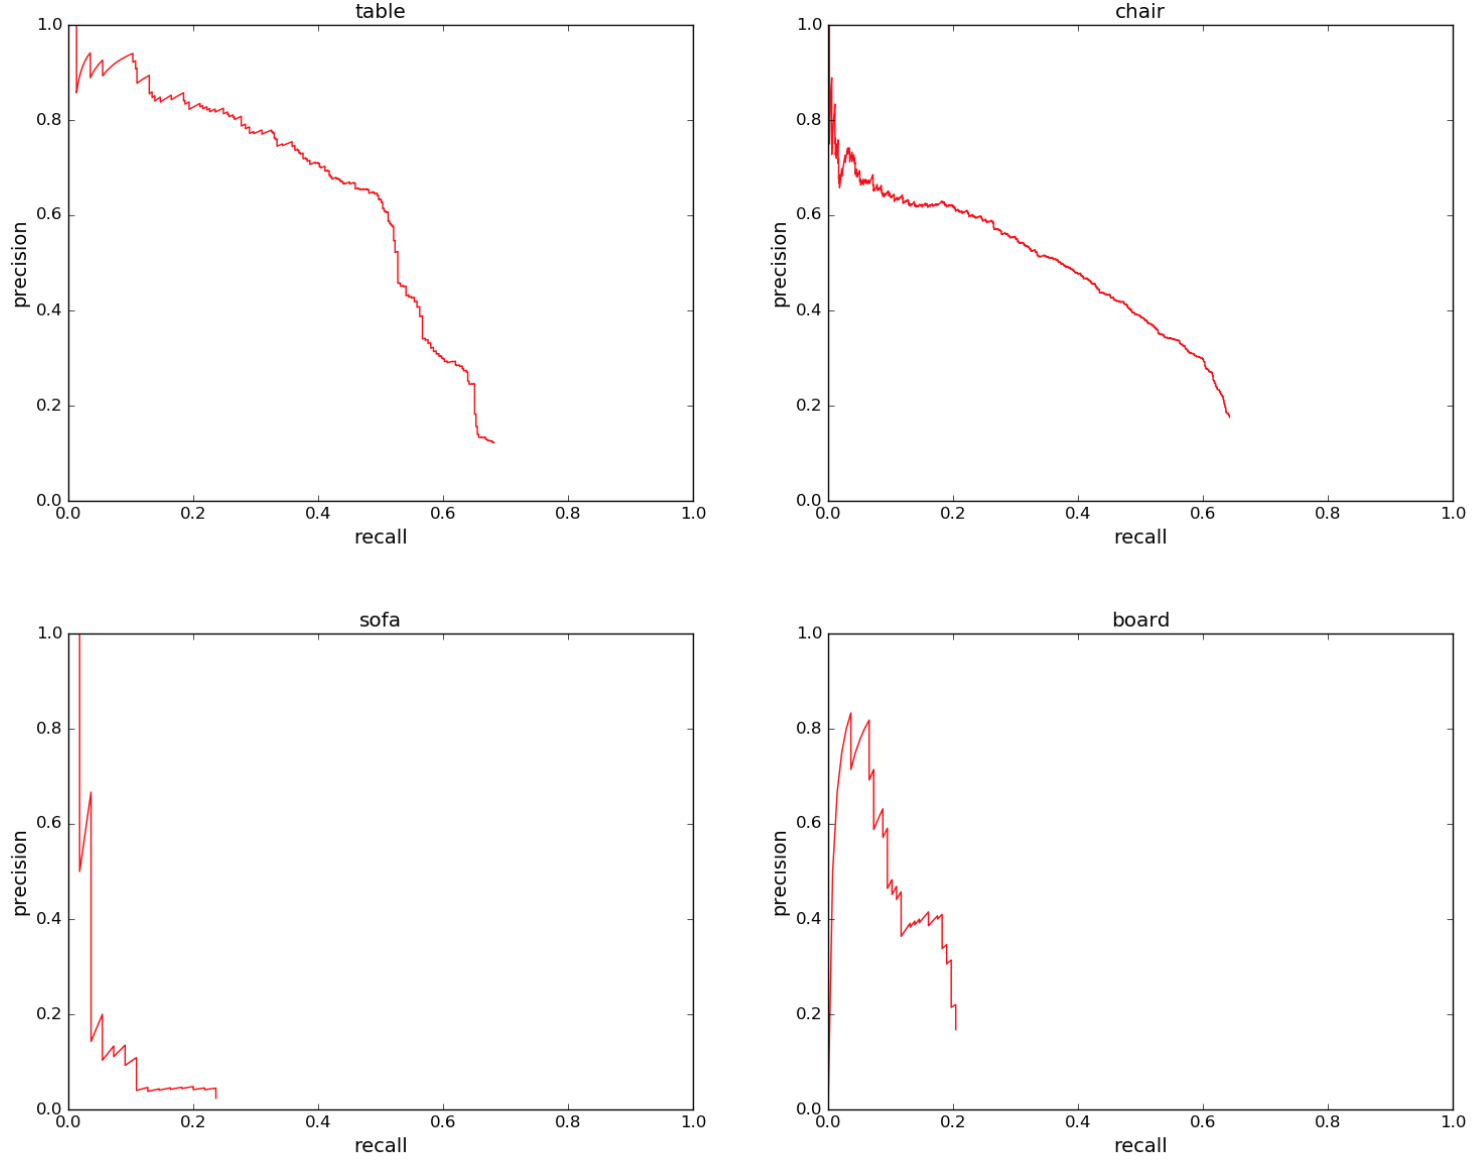
\includegraphics[width=0.8\linewidth]{fig/pr_curve.png}
 \centering
 \caption{\textbf{用于 3D 点云中对象检测的准确率-召回率曲线。} 我们在所有的六个区域上对四个类别进行了评估:桌子、椅子、沙发和木板。 IoU 阈值在体积上表现为 0.5 。}
 \label{fig:pr_curve}
 \end{figure}
 
% =============================
% More Applications
% =============================
\section{更多应用 (Sec 5.1)}
\label{sec:supp_application}
\paragraph{从点云中检索模型} 我们的 PointNet 为每个给定的输入点云学习全局形状特征。我们期望几何相似的形状具有相似的全局特征。在本节中,我们将在形状检索应用程序上测试我们的猜想。更具体地说,对于由 ModelNet 划分的测试集中每个给定查询形状,我们计算其由我们的分类 PointNet 给出的全局签名(分数预测层之前的层的输出),并通过最近邻搜索在划分的训练集中检索相似的形状。结果如图~\ref{fig:retrieval}所示。

\begin{figure}[h]
    \centering
    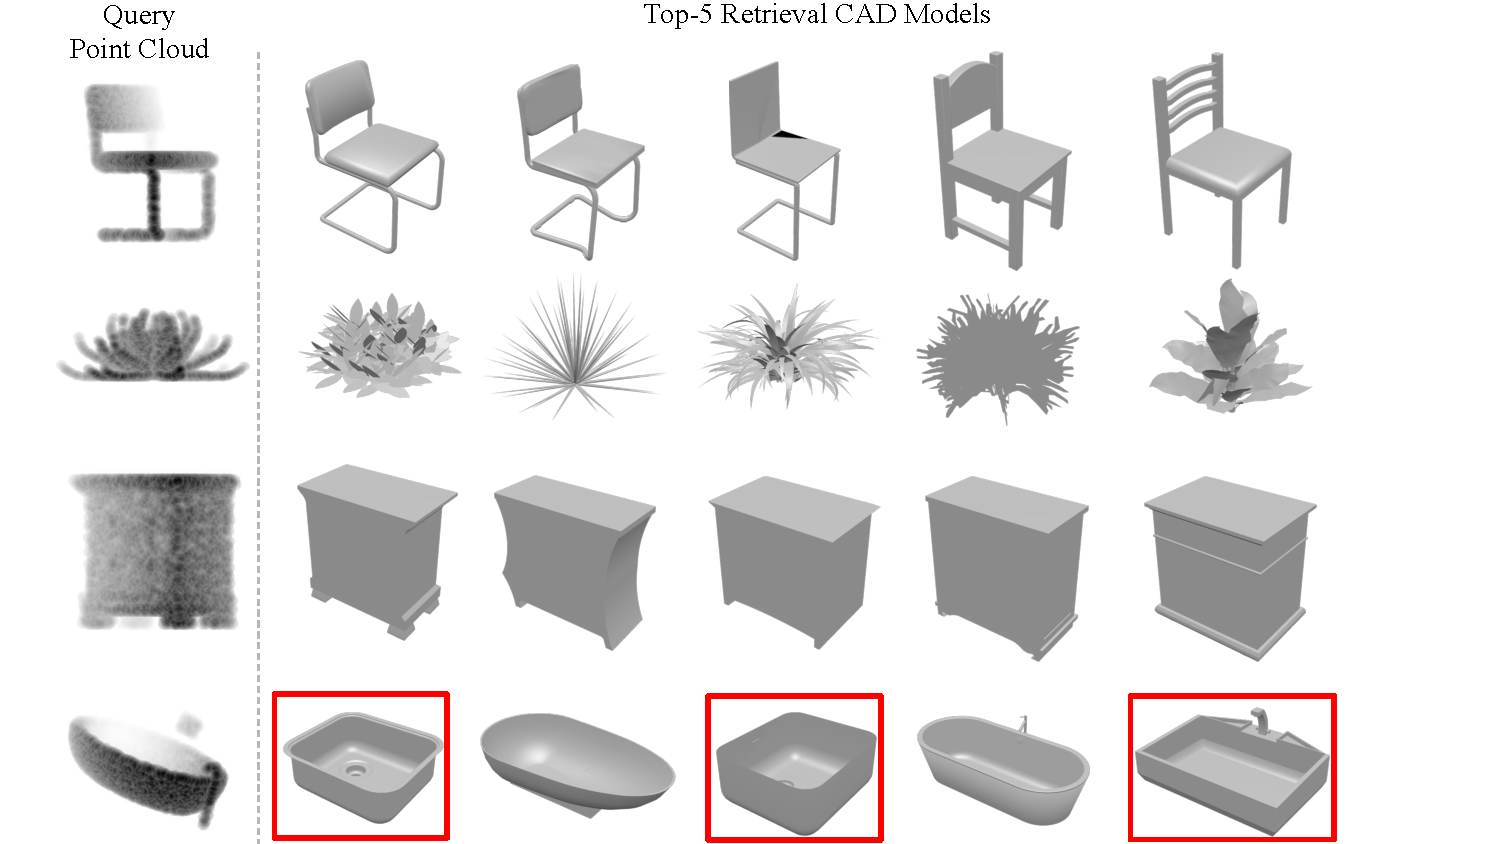
\includegraphics[width=\linewidth]{fig/retrieval.pdf}
    \caption{\textbf{从点云中检索模型。} 对于每个给定的点云,我们从 ModelNet 划分的测试集中检索前 5 个相似的形状。 从上到下,我们展示了椅子、植物、床头柜和浴缸查询的示例。错误类别的检索结果用红色框标记。}
    \label{fig:retrieval}
\end{figure}

\paragraph{形状对应}
%Since our PointNet learns many per-point functions at the first stage and then aggregates the computed per-point features together using a max-pooling to compute the global shape feature. Thus, there is an inherent correspondence between every coordinate of the global features for a pair of shapes. 

在本节中,我们展示了 PointNet 学习的点特征可以潜在地用于计算形状对应。 给定两个形状,我们通过匹配激活全局特征中相同维度的点对来计算它们的 \textit{critical point sets} $C_S$ 之间的对应关系。Fig~\ref{fig:chair_corr} 和 Fig~\ref{fig:table_corr} 显示了检测到的两个相似椅子和桌子之间的形状对应关系。

\begin{figure}[h]
    \centering
    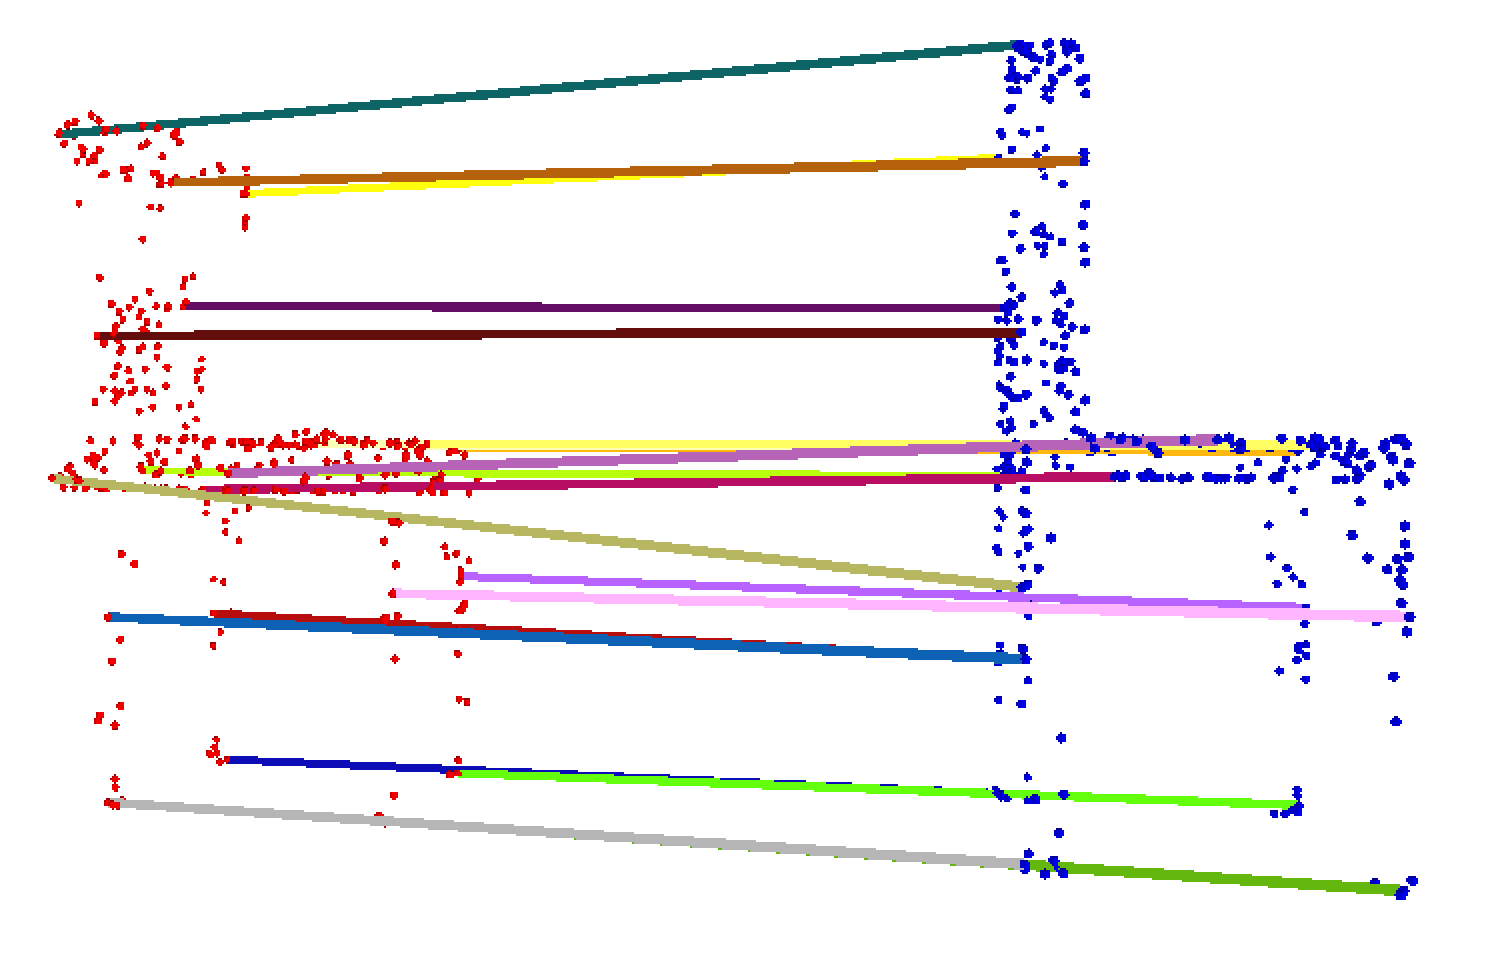
\includegraphics[width=\linewidth]{fig/chair_corr.png}
    \caption{\textbf{两个椅子之间的形状对应。} 为了可视化的清晰性,我们只展示了 20 个随机挑选的映射对。}
    \label{fig:chair_corr}
\end{figure}

\begin{figure}[h]
    \centering
    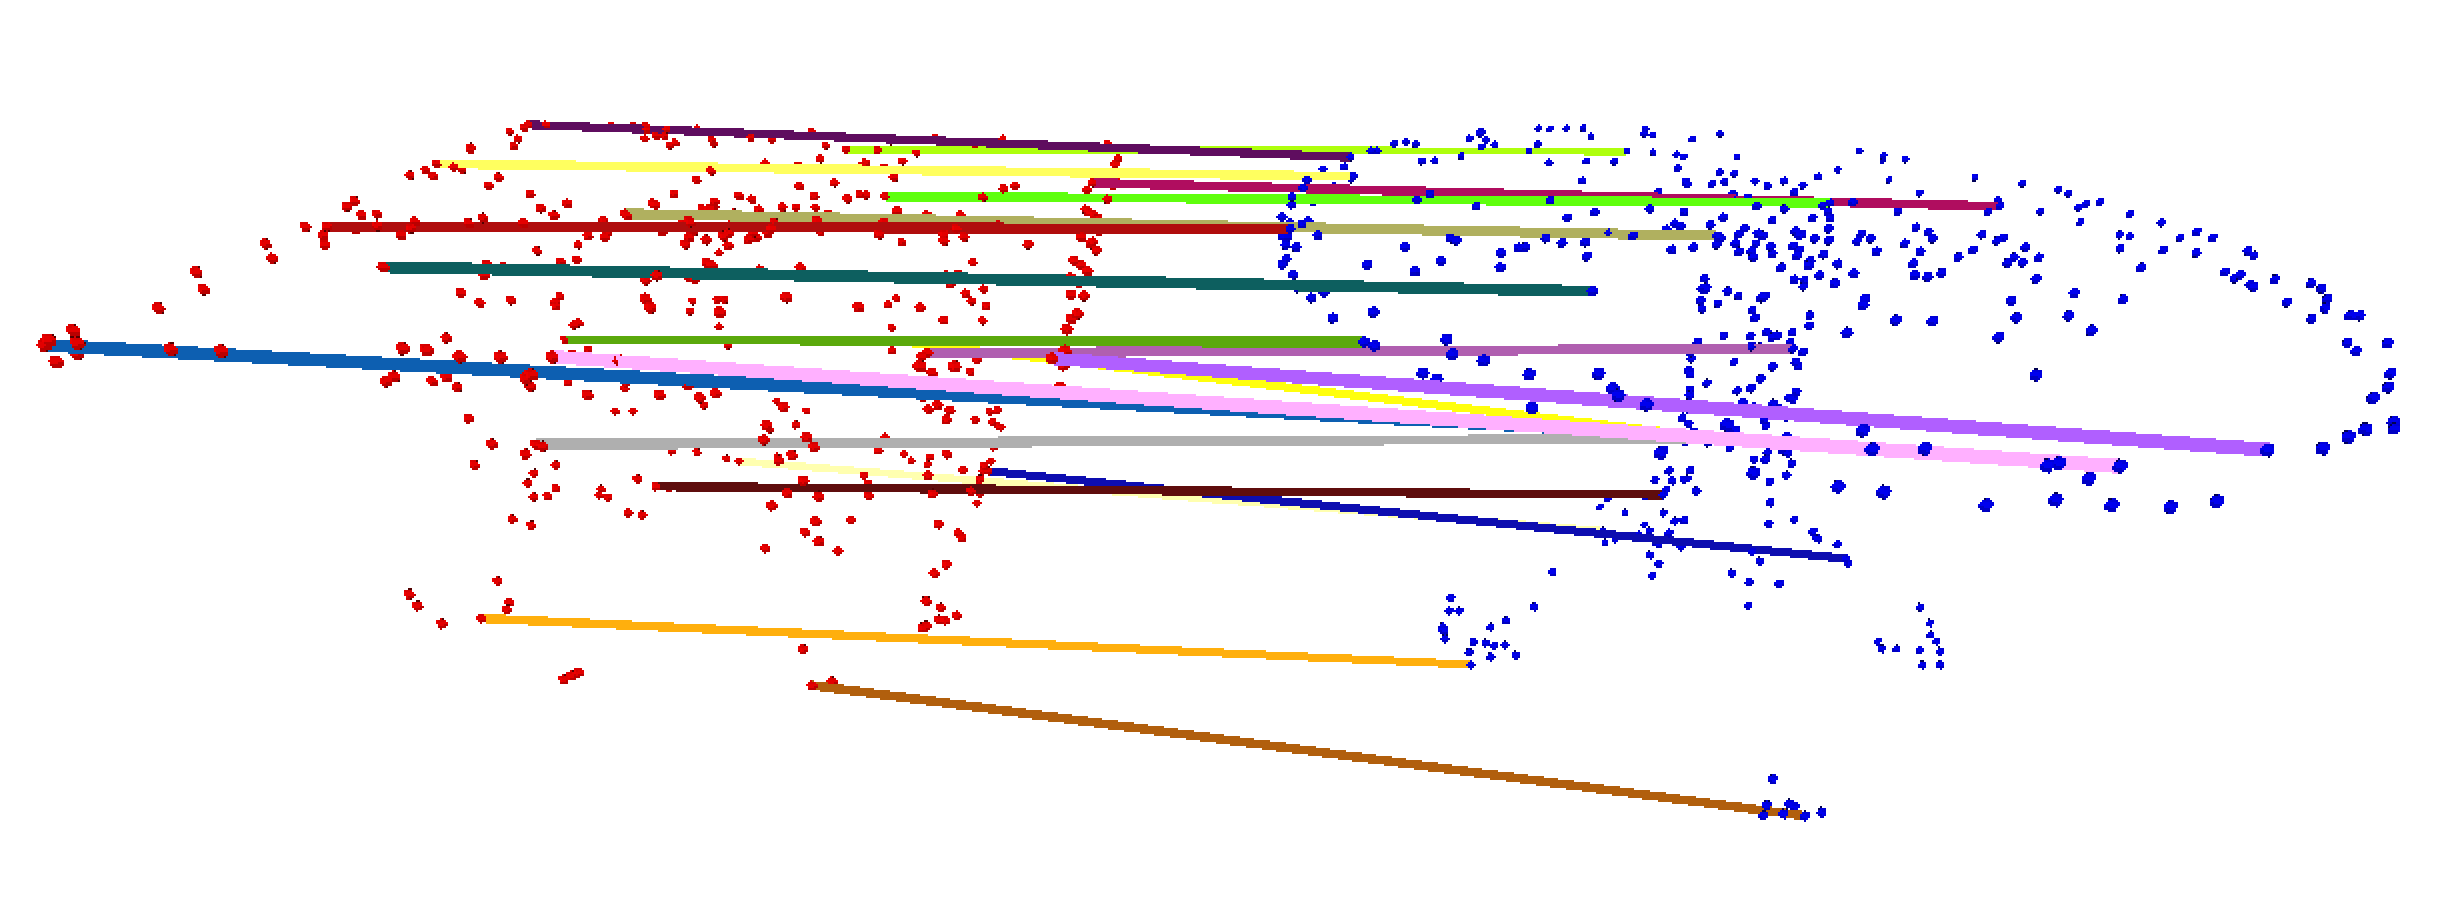
\includegraphics[width=\linewidth]{fig/table_corr.png}
    \caption{\textbf{两张桌子之间的形状对应。} 为了可视化的清晰性,我们只展示了 20 个随机挑选的映射对。}
    \label{fig:table_corr}
\end{figure}


% =============================
% More Architecture Analysis
% =============================
\section{更多结构分析 (Sec 5.2)}
\label{sec:architecture}
% \paragraph{Volumetric Reconstruction} To validate proof under Thm2 saying that in the worst case our network will degrade to learn a volumetric respentation for the 3D shape? 

\paragraph{瓶颈维度和输入点数量的有效性}

根据第一个输入层的大小和输入点云的数量,我们的模型的表现会有所变化,接下来我们将阐释其变化。 从图 ~\ref{fig:net_param} 中我们可以看出,随着我们提高点的数量,性能变得越来越好。在大约 1000 个点时,达到饱和。最大的层尺寸同样起了重要作用,让我们将层大小从 64 增大到 1024 之后,表现提升了 $2-4\%$。这说明我们需要足够多的,覆盖整个三维空间的点特征函数来分辨不同的形状。



% \paragraph{Effects of Bottleneck Dimension and Number of Input Points}
% Here we show our model's performance change with regard to the size of the first max layer output as well as the number of input points. In Fig~\ref{fig:net_param} we see that performance grows as we increase the number of points however it saturates at around 1K points. The max layer size plays an important role, increasing the layer size from 64 to 1024 results in a $2-4\%$ performance gain. It indicates that we need enough point feature functions to cover the 3D space in order to discriminate different shapes.

值得一提的是,即便有 64 个点作为了输入(从网络上采样的点中最远的点),我们的网络仍然能够取得令人满意的效果。

% It's worth notice that even with 64 points as input (obtained from furthest point sampling on meshes), our network can achieve decent performance.

\begin{figure}[h]
    \centering
    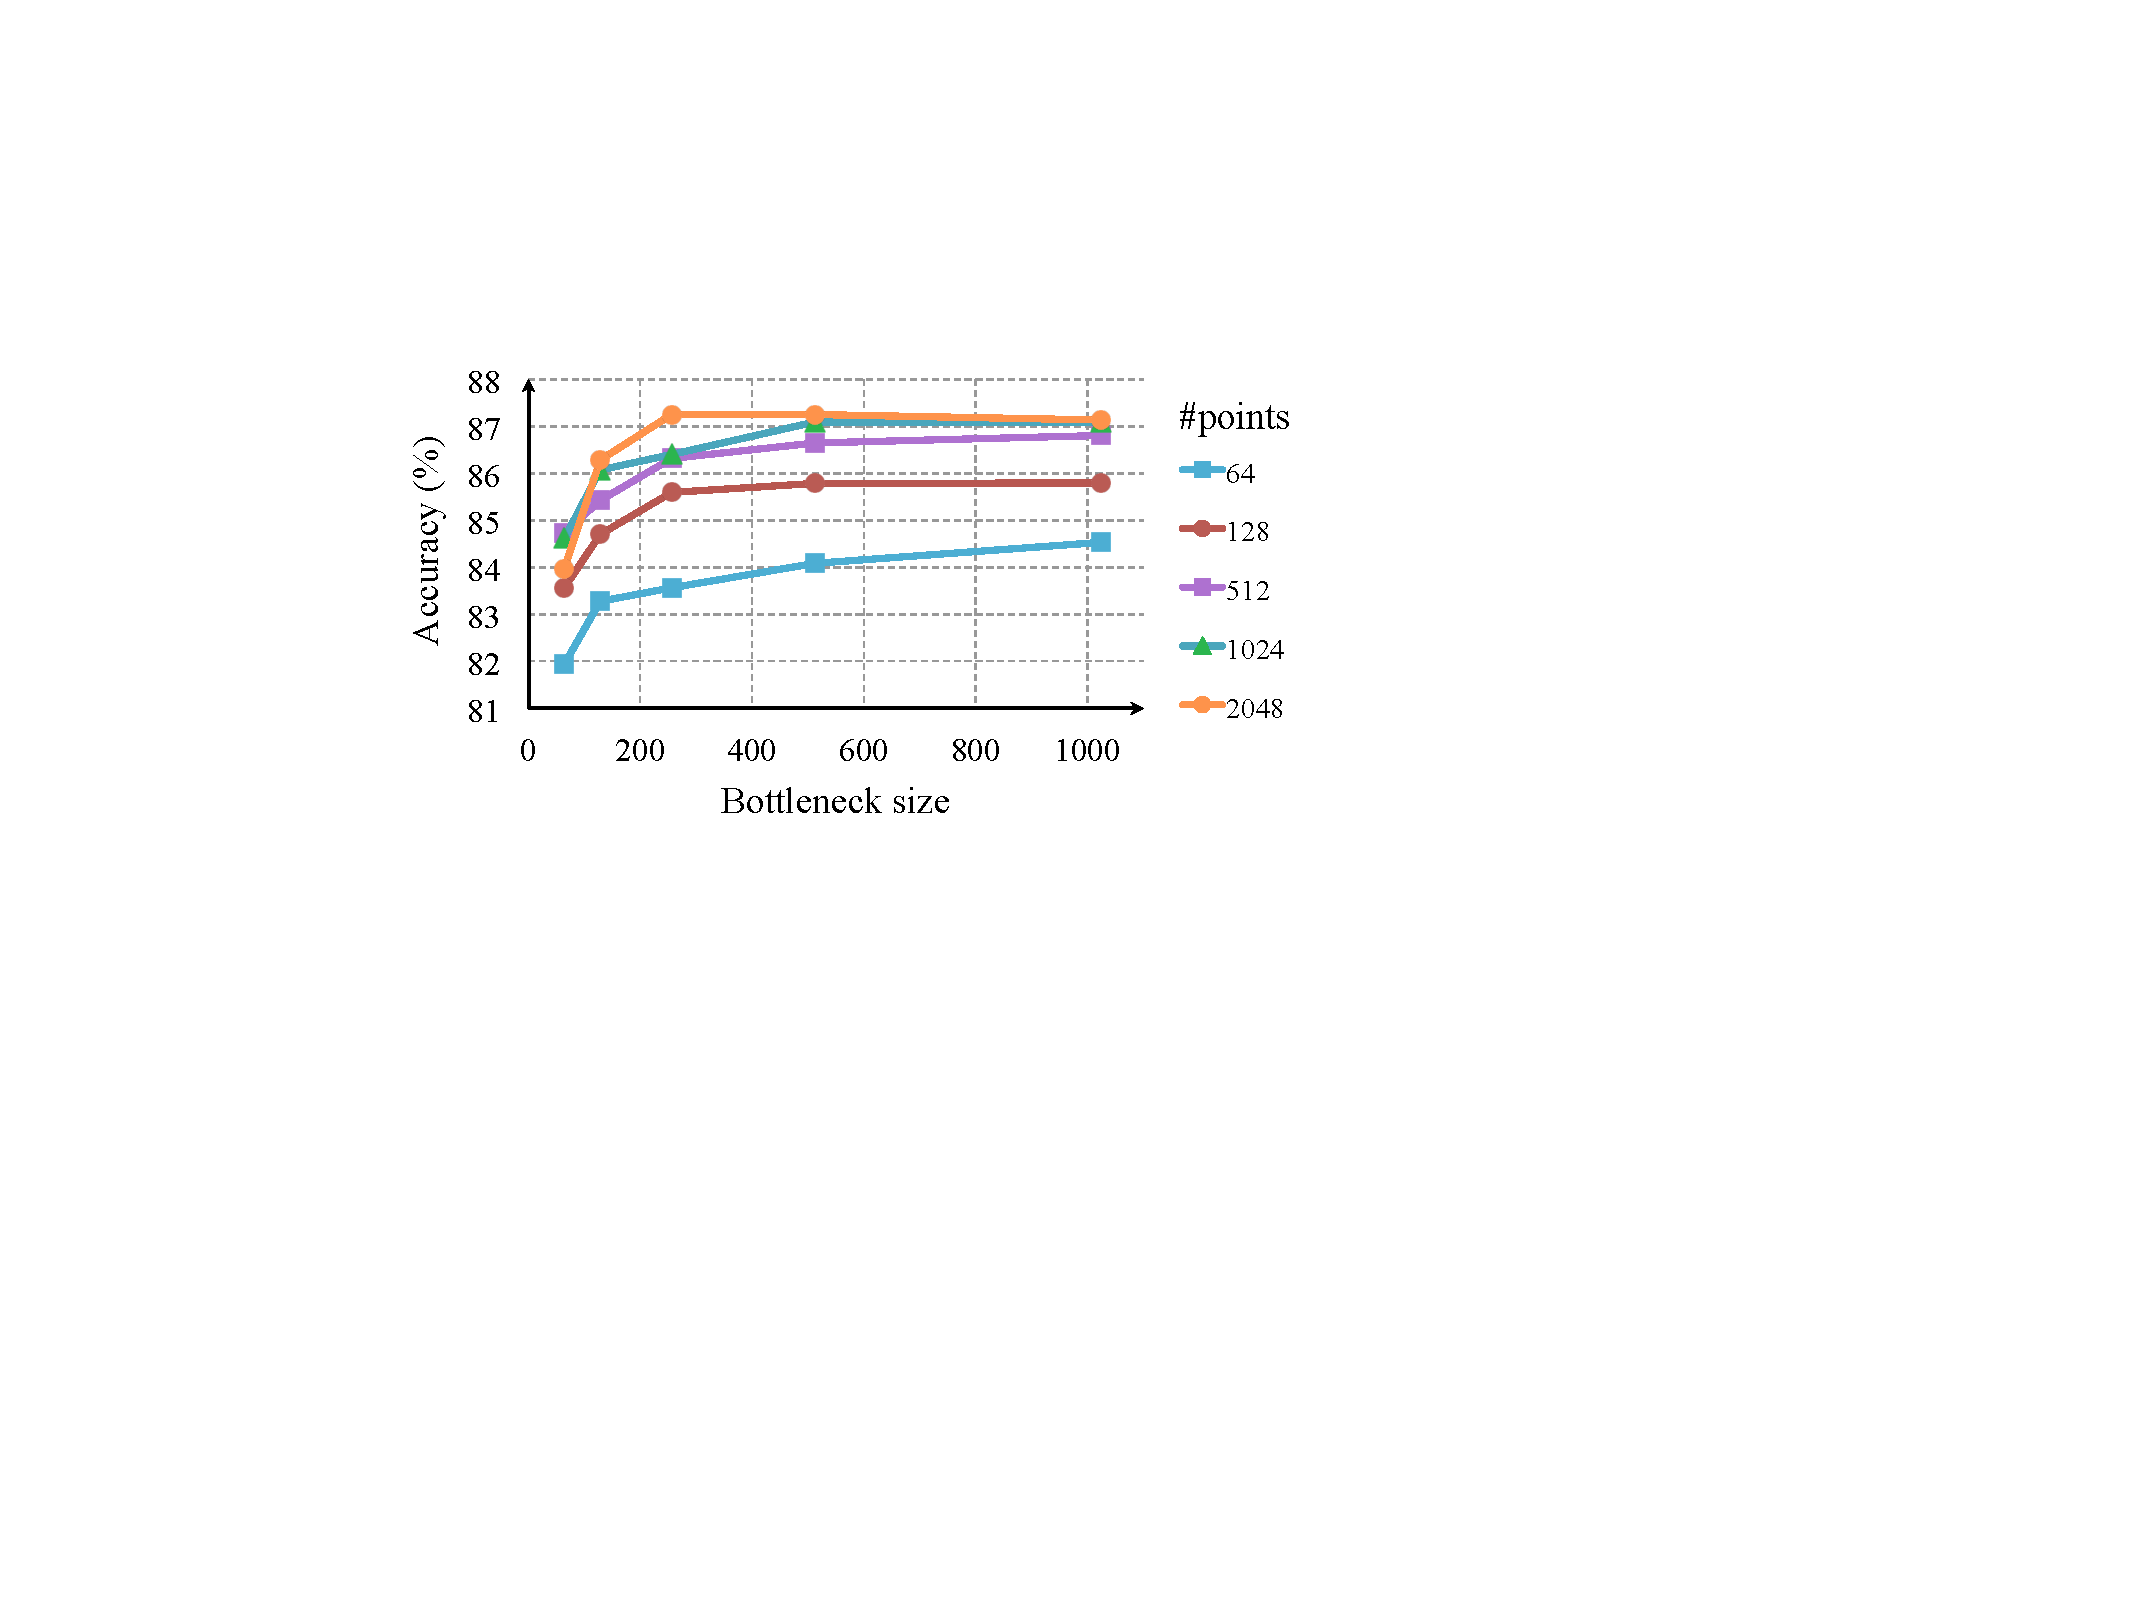
\includegraphics[width=0.8\linewidth]{fig/bottleneck.pdf}
    \caption{\textbf{瓶颈尺寸和输入点数量的效果} 该指标为 ModelNet40 上的总体的分类准确度。}
    \label{fig:net_param}
\end{figure}

\paragraph{MNIST 数字分类} 在我们关注 3D 点云的学习的同时,我们在用我们的网络在 2D 点云上做了实验,即像素集。

% \paragraph{MNIST Digit Classification}
% While we focus on 3D point cloud learning, a sanity check experiment is to apply our network on a 2D point clouds - pixel sets.

为了将一个 MNIST 图像转换成一个 2D 点云,我们设置了阈值像素值,将所有值大于 128 的像素(用图像中的 $(x,y)$ 坐标表示)加入到集合中。我们使用了一个大小为 256 的集合大小。如果集合中有多于 256 个像素,我们就从中随机地抽样;如果集合中的元素少于 256 个,我们便用集合中存在的点来做填充(由于我们的最大化操作,使用哪一个点来填充并不会影响结果)。

% To convert an MNIST image into a 2D point set we threshold pixel values and add the pixel (represented as a point with $(x,y)$ coordinate in the image) with values larger than 128 to the set. We use a set size of 256. If there are more than 256 pixels int he set, we randomly sub-sample it; if there are less, we pad the set with the one of the pixels in the set (due to our max operation, which point to use for the padding will not affect outcome).

如表 ~\ref{tab:mnist} 所示,我们将其和若干个基准线进行比较(包括将输入图像作为有序向量的多层感知机、将输入图像作为一个从 (0,0) 像素到 (27,27) 像素的循环神经网络、以及一个简易的卷积神经网络)。虽然其中表现最好的模型仍然是一个仔细调试过的卷积神经网络(达到了低于 $0.3\%$ 的错误率),但 PointNet 的表现在二维点集上的表现已经符合预期。

% As seen in Table~\ref{tab:mnist}, we compare with a few baselines including multi-layer perceptron that considers input image as an ordered vector, a RNN that consider input as sequence from pixel (0,0) to pixel (27,27), and a vanilla version CNN. While the best performing model on MNIST is still well engineered CNNs (achieving less than $0.3\%$ error rate), it's interesting to see that our PointNet model can achieve reasonable performance by considering image as a 2D point set.

% vanila CNN: https://www.microsoft.com/en-us/research/publication/best-practices-for-convolutional-neural-networks-applied-to-visual-document-analysis/

\begin{table}[h!]
    \centering
    \begin{tabular}[width=\linewidth]{l|c|c}
    \hline
    ~                      & 输入 & 错误率 (\%) \\ \hline
    多层感知机~\cite{simard2003best} & vector & 1.60  \\
    LeNet5~\cite{lecun1998gradient}                 & image & 0.80 \\ \hline
    我们的 PointNet          & point set & 0.78 \\ \hline
    \end{tabular}
    \caption{\textbf{MNIST 分类结果} 我们将我们的模型和其他简单的深度学习结构进行比对,从而说明我们的模型在二维点云上的表现仍然符合预期。
    % We compare with vanilla versions of other deep architectures to show that our network based on point sets input is achieving reasonable performance on this traditional task.
    }
    \label{tab:mnist}
\end{table}


\paragraph{法线预测}
在分割版本的 PointNet 中,为了为局部的点提供上下文信息,局部的点特征与全局的点特征被拼接在了一起。但这种拼接方式不能保证模型学习到上下文。在该实验中,我们通过展示我们的分割网络具备预测点法线(一个由某个点的邻居所决定的局部几何特征)的能力,来验证我们的设计。

% \paragraph{Normal Estimation}
% In segmentation version of PointNet, local point features and global feature are concatenated in order to provide context to local points. However, it's unclear whether the context is learnt through this concatenation. In this experiment, we validate our design by showing that our segmentation network can be trained to predict point normals, a local geometric property that is determined by a point's neighborhood.

%Our proposed PointNet learns 1024 per-point functions and uses a max-pooling operation to aggregate the per-point features into the global shape feature. Then for classification task, we push this learnt global shape signature to the subsequent classifier. The jump for per-point feature (extremely local) to the shape feature (extremely global) seems fine. However, for segmentation task, one may wonder if the local context entails crucial information to determine the local fine-grained segmentation details. Even though in our segmentation version PointNet we concatenate the learn global shape signature and the per-point local features together to do the label predictions, it is still unclear if such combination can capture the necessary local information around each point. 

我们用一种监督学习的方式修改并训练了我们的分割 PointNet 来回归到真正的点法线。我们仅仅改变了分割 PointNet 的最后一层,使其为每一个点预测法向量。对于损失函数,我们使用了余弦距离的绝对值。

% We train a modified version of our segmentation PointNet in a supervised manner to regress to the ground-truth point normals. We just change the last layer of our segmentation PointNet to predict normal vector for each point. We use absolute value of cosine distance as loss.

图 ~\ref{fig:normal_recon} 对比了我们的 PointNet 法线预测结果(左)和从网格中计算出来的真正的法线(右)。从图中可以看到,我们得到了一个合理的法线重建结果。在一些区域,我们的预测结果甚至比真正的法线(通常包括一些翻转了的法线方向)更加平滑和连续。

% Fig.~\ref{fig:normal_recon} compares our PointNet normal prediction results (the left columns) to the ground-truth normals computed from the mesh (the right columns). We observe a reasonable normal reconstruction. Our predictions are more smooth and continuous than the ground-truth which includes flipped normal directions in some region.
%Having the ability to correctly predict the point normal, one of the local geometric features that require the combination of the information of a point and its neighbors, shows our PointNet has the potential to capture the local information via simply combining the per-point feature and the aggregated global feature.

\begin{figure}[t!]
\centering
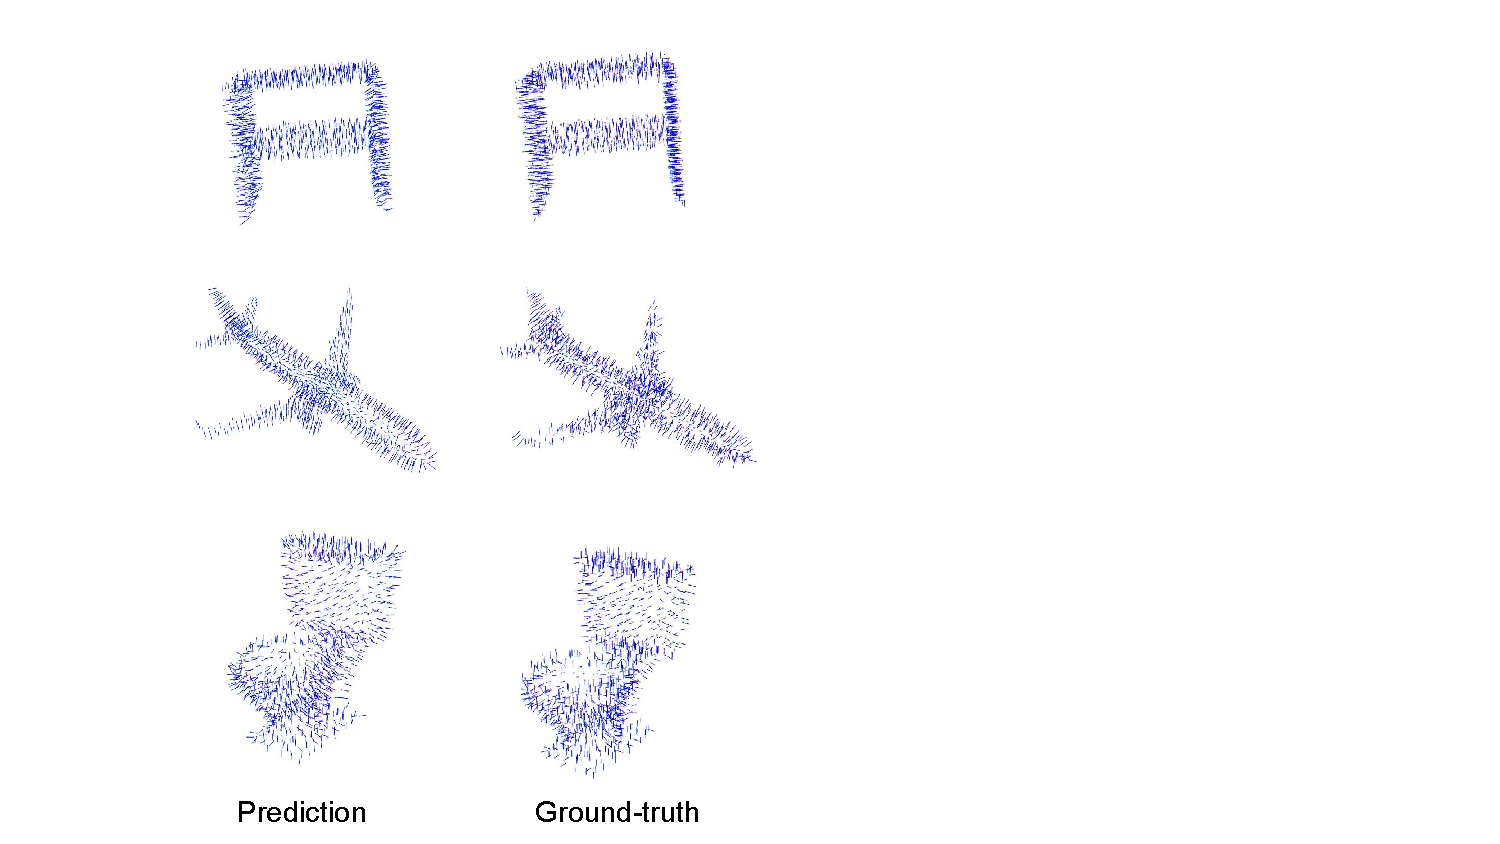
\includegraphics[width=0.9\linewidth]{fig/normal_recon2.pdf}
\caption{\textbf{PointNet 法线重建结果。} 改图展示了在一个示例点云中所有点的法线重建结果与从网格中计算出来的真正的法线结果。}
\label{fig:normal_recon}
\end{figure}


\paragraph{分割健壮性} 如 5.2 和 ~\ref{sec:cla_robust} 讨论,由于全局的形状特征是从一些 \textit{关键点} 中提取出来的,我们的点云对于数据干扰和点的缺失并不敏感。在这一部分中,我们展示了我们的模型在面对分割任务时,仍然保持着健壮性。每一个点的标签是根据两部分来预测的:各个点的特征的结合,与模型学习到的全局形状特征。在图 ~\ref{fig:seg_robust} 中,我们展示了给定输入点云 $S$ (左)的分割结果、\textit{关键点集} $\mathcal{C}_S$ (中)和 \textit{上界形状} $\mathcal{N}_S$。

% \paragraph{Segmentation Robustness} As discussed in Sec 5.2 and Sec~\ref{sec:cla_robust}, our PointNet is less sensitive to data corruption and missing points for classification tasks since the global shape feature is extracted from a collection of \textit{critical points} from the given input point cloud. In this section, we show that the robustness holds for segmentation tasks too. The per-point part labels are predicted based on the combination of per-point features and the learnt global shape feature. In Fig~\ref{fig:seg_robust}, we illustrate the segmentation results for the given input point clouds $S$ (the left-most column), the \textit{critical point sets} $\mathcal{C}_S$ (the middle column) and the \textit{upper-bound shapes} $\mathcal{N}_S$.

%One may observe that the segmentation results for the entire shape family containing all the shapes transiting between $\mathcal{C}_S$ and $\mathcal{N}_S$ are consistent, meaning that \textbf{losing some points that are not \textit{critical} does not affect the segmentation result}.

\begin{figure}[t!]
\centering
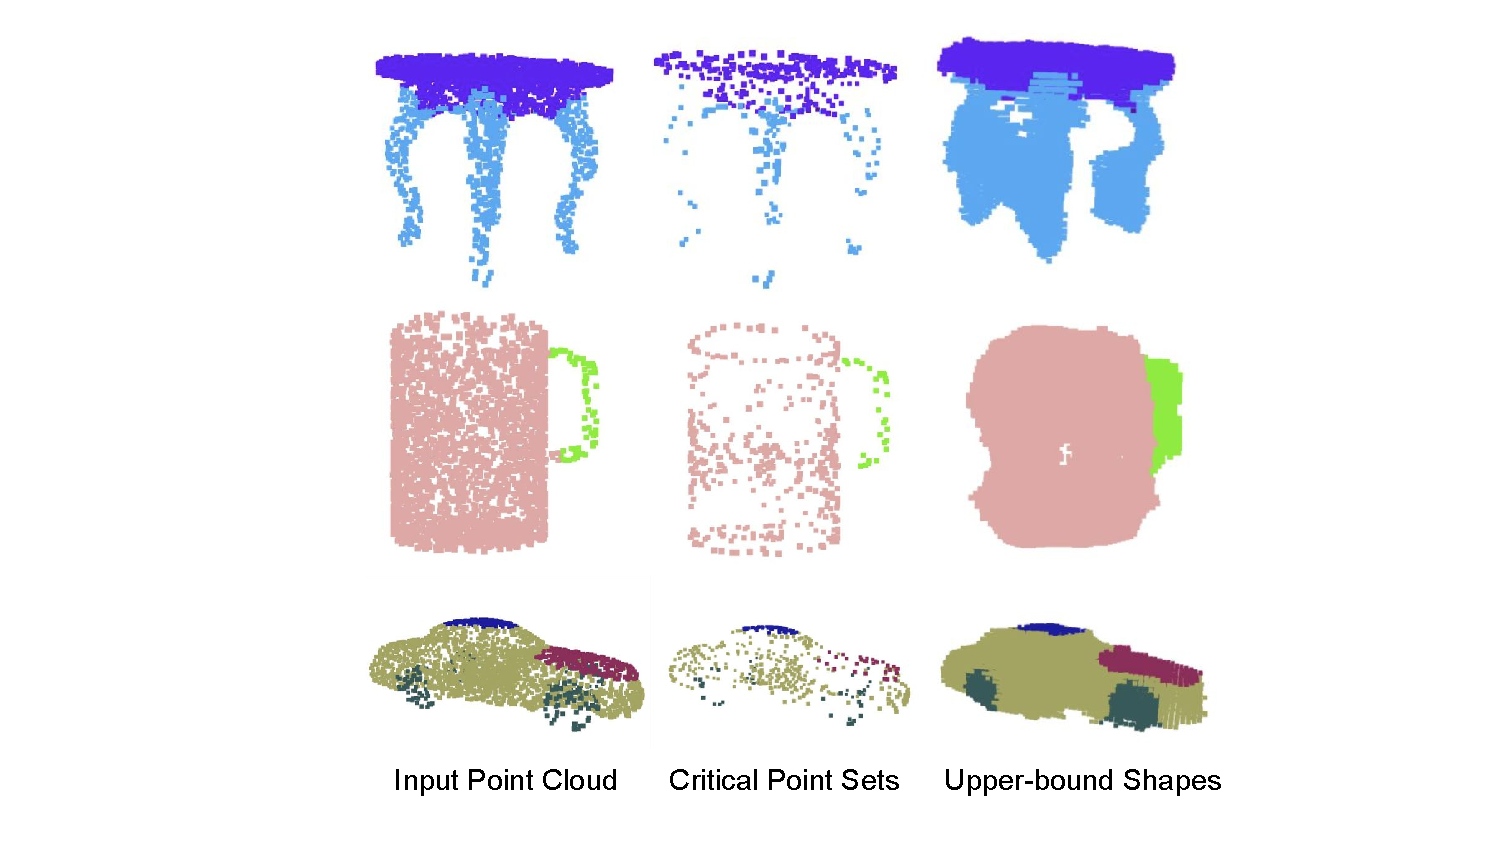
\includegraphics[width=0.9\linewidth]{fig/seg_robust.pdf}
\caption{\textbf{分割结果的一致性} 我们用图例说明一些样例物体点云的\textit{关键点集} $\mathcal{C}_S$和\textit{上界形状} $\mathcal{N}_S$ 的分割结果。 可以得出从$\mathcal{C}_S$ 到 $\mathcal{N}_S$ 的形状簇拥有共同的分割结果。}
\label{fig:seg_robust}
\end{figure}

% \begin{comment}

在 5.2 \textit{三维物体零件分割}中,我们将我们提出的 PointNet 模型应用在了 CAD 模型的语义零件分割上。我们的分割 PointNet(如图 2 \textit{分割网络})在完整的 ShapeNet 网络上达到了最优的效果。意料之中的,我们的模型在局部数据(如:模拟的 Kinect 扫描结果)中也表现的很好。由于真实世界中的扫描通常因为遮挡问题而变得十分不完整,模型在面对局部输入时的健壮性非常重要,是评估其实际应用价值的关键。表 ~\ref{tab:segmentation_partial} 概括了在面对完整的和局部的数据时,我们的 PointNet 与作为基准线的三维卷积神经网络方法得出的效果。

% In Sec 5.2 \textit{3D Object Part Segmentation}, we apply our proposed PointNet on segmenting the CAD models into semantic parts. While our segmentation PointNet (illustrated in Fig. 2, \textit{Segmentation Network}) achieves the state-of-the-art result on complete ShapeNet shapes, it performs reasonably well on partial data (e.g. simulated Kinect scans) as well. Since most real world scans are very partial due to occlusions, a model's robustness to partial input is key to evaluate its value in practice. Table~\ref{tab:segmentation_partial} summarizes the performance of our PointNet and the proposed baseline 3D CNN method when being applied to complete and partial data.


\begin{table}[h!]
    \small
    \centering
    \begin{tabular}[width=\linewidth]{l|cccc}
    \hline
    ~ & 完整输入 & 局部输入 \\ \hline
    3D CNN & 75.3 & 69.7 \\ \hline
    Ours PointNet & \textbf{80.6} & \textbf{75.3}  \\ \hline
    \end{tabular}
    \caption{\textbf{局部扫描的分割结果} 衡量指标为所有形状的 mIoU。在完整数据上训练我们的点网络时,我们进行了旋转增强,以便与从多个角度生成的模拟Kinect扫描进行公平的比较。两个网络分别在完整数据和部分数据上进行训练,然后在不同的子测试集上进行了测试。}
    \label{tab:segmentation_partial}
\end{table}

% \begin{table}[h!]
%     \small
%     \centering
%     \begin{tabular}[width=\linewidth]{l|cccc}
%     \hline
%     ~ & 完整输入 & 局部输入 \\ \hline
%     3D CNN & 75.3 & 69.7 \\ \hline
%     Ours PointNet & \textbf{80.6} & \textbf{75.3}  \\ \hline
%     \end{tabular}
%     \caption{\textbf{Segmentation results on partial scans.} Metric is mean IoU across all shapes. We perform rotation augmentation when training our PointNet on complete data to fairly compare with the simulated Kinect scans, that are generated from multiple perspective. Both networks are trained respectively on the complete data and the partial data and then tested on the testing splits.}
%     \label{tab:segmentation_partial}
% \end{table}

% \end{comment}

\paragraph{网络面对未知形状分类的通用性}
在图 \ref{fig:unseen} 中,我们可视化了 \textit{关键点集} 和 \textit{上界形状} 在面对来自从未出现在 ModelNet 或 ShapeNet 中的未知分类(脸部、马、兔子、茶壶)的新性状。结果表明,我们的模型学习到的各个点的函数是具备通用性的。然而,由于我们主要使用具备大量平面结构的人造物品来训练模型,重建出来上界形状同样也包含了更多的平面表面。

% In Fig~\ref{fig:unseen}, we visualize the \textit{critical point sets} and the \textit{upper-bound shapes} for new shapes from unseen categories (face, house, rabbit, teapot) that are not present in ModelNet or ShapeNet. It shows that the learnt per-point functions are generalizable. However, since we train mostly on man-made objects with lots of planar structures, the reconstructed upper-bound shape in novel categories also contain more planar surfaces. 
 


% \paragraph{Network Generalizability to Unseen Shape Categories}
% %As discussed in the previous sections, our proposed PointNet learns several useful per-point functions and computes the global shape signature by max pooling all the point features.
% %In Sec 5.3, we visualize the learnt per-point functions and observe that they work in the way to detect if some points intersect with some specific regions. And, by aggregating the learnt per-point features, PointNet selects some \textit{critical points} and produces the global shape feature by summarizing the activation values of them.
% In Fig~\ref{fig:unseen}, we visualize the \textit{critical point sets} and the \textit{upper-bound shapes} for new shapes from unseen categories (face, house, rabbit, teapot) that are not present in ModelNet or ShapeNet. It shows that the learnt per-point functions are generalizable. However, since we train mostly on man-made objects with lots of planar structures, the reconstructed upper-bound shape in novel categories also contain more planar surfaces. 
 
\begin{figure}[t!]
\centering
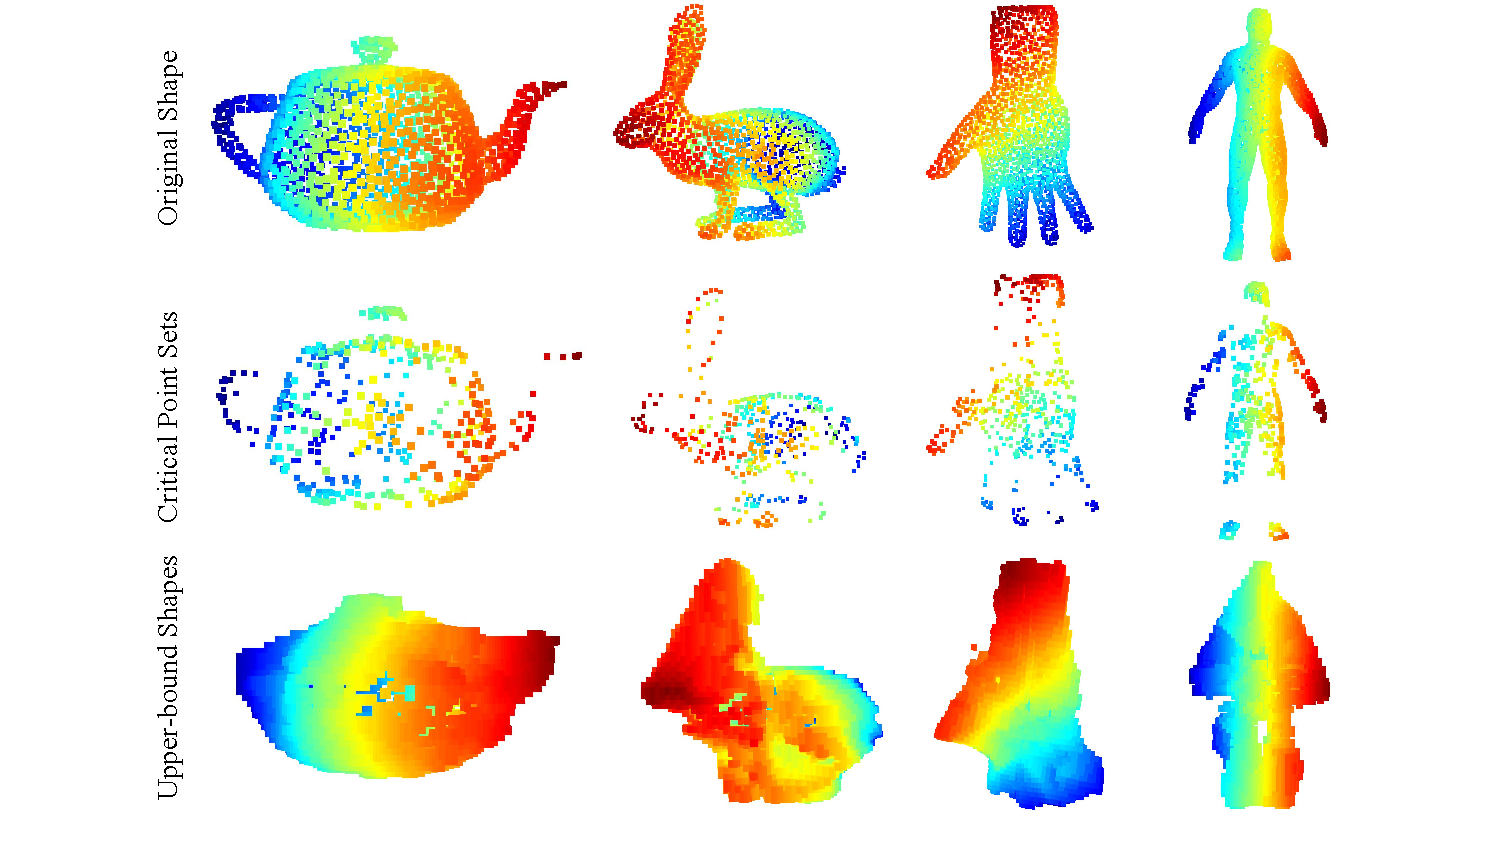
\includegraphics[width=\linewidth]{fig/unseen.pdf}
\caption{\textbf{未知物体的关键点集和上界形状} 我们可视化了茶壶,兔子,手,人体的 \textit{关键点集} 和 \textit{上界形状}。 通过这些不在ModelNet和ShapeNet数据集的物体来测试PointNet学习到的点函数的通用性。图中用颜色编码反应深度信息。}
\label{fig:unseen}
\end{figure}

\section{定理证明 (Sec 4.3)}
\label{sec:proof}
\input{./tex/appendix}


\begin{figure}[h!]
    \centering
    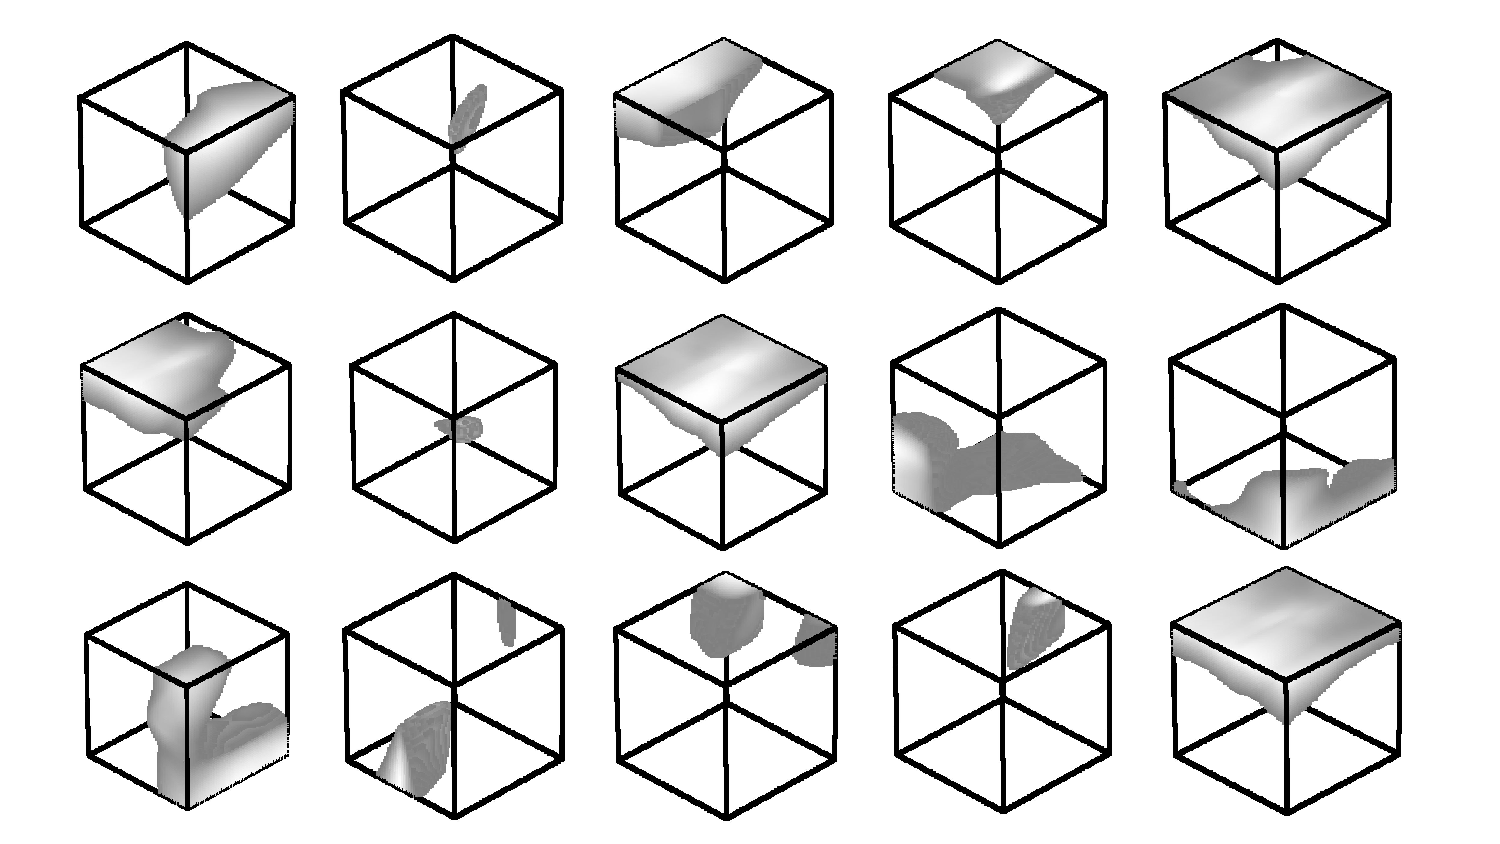
\includegraphics[width=0.7\linewidth]{fig/kernels.pdf}
    \caption{\textbf{点函数可视化} 对于每个点函数$h$,计算位于原点的边长为2的立方体中每个点$p$的$h(p)$值 , 该区域覆盖了训练PointNet时输入数据规范化的单位球区域。 在这幅图中, 我们可视化所有$h(p)>0.5$的点$p$,函数值用体素亮度表示。 我们随机选取15个点函数并可视化其活跃区域。}
    \label{fig:functions}
\end{figure}

\section{更多的可视化}
\label{sec:visu}
\paragraph{分类可视化}
%In this section, we investigate the classification version PointNet, visualize the shape global feature space via 2D embedding and provide some error analysis on the failure cases.

我们使用t-SNE\cite{maaten2008visualizing}把从我们的分类PointNet中得到的点云全局结果(1024-dim)降维嵌入到2D空间中。图~\ref{fig:tsne}显示了ModelNet40用于测试的分割形状的嵌入空间。相似的形状根据它们的语义类别分别聚集到一起。

\begin{figure*}[t!]
\centering
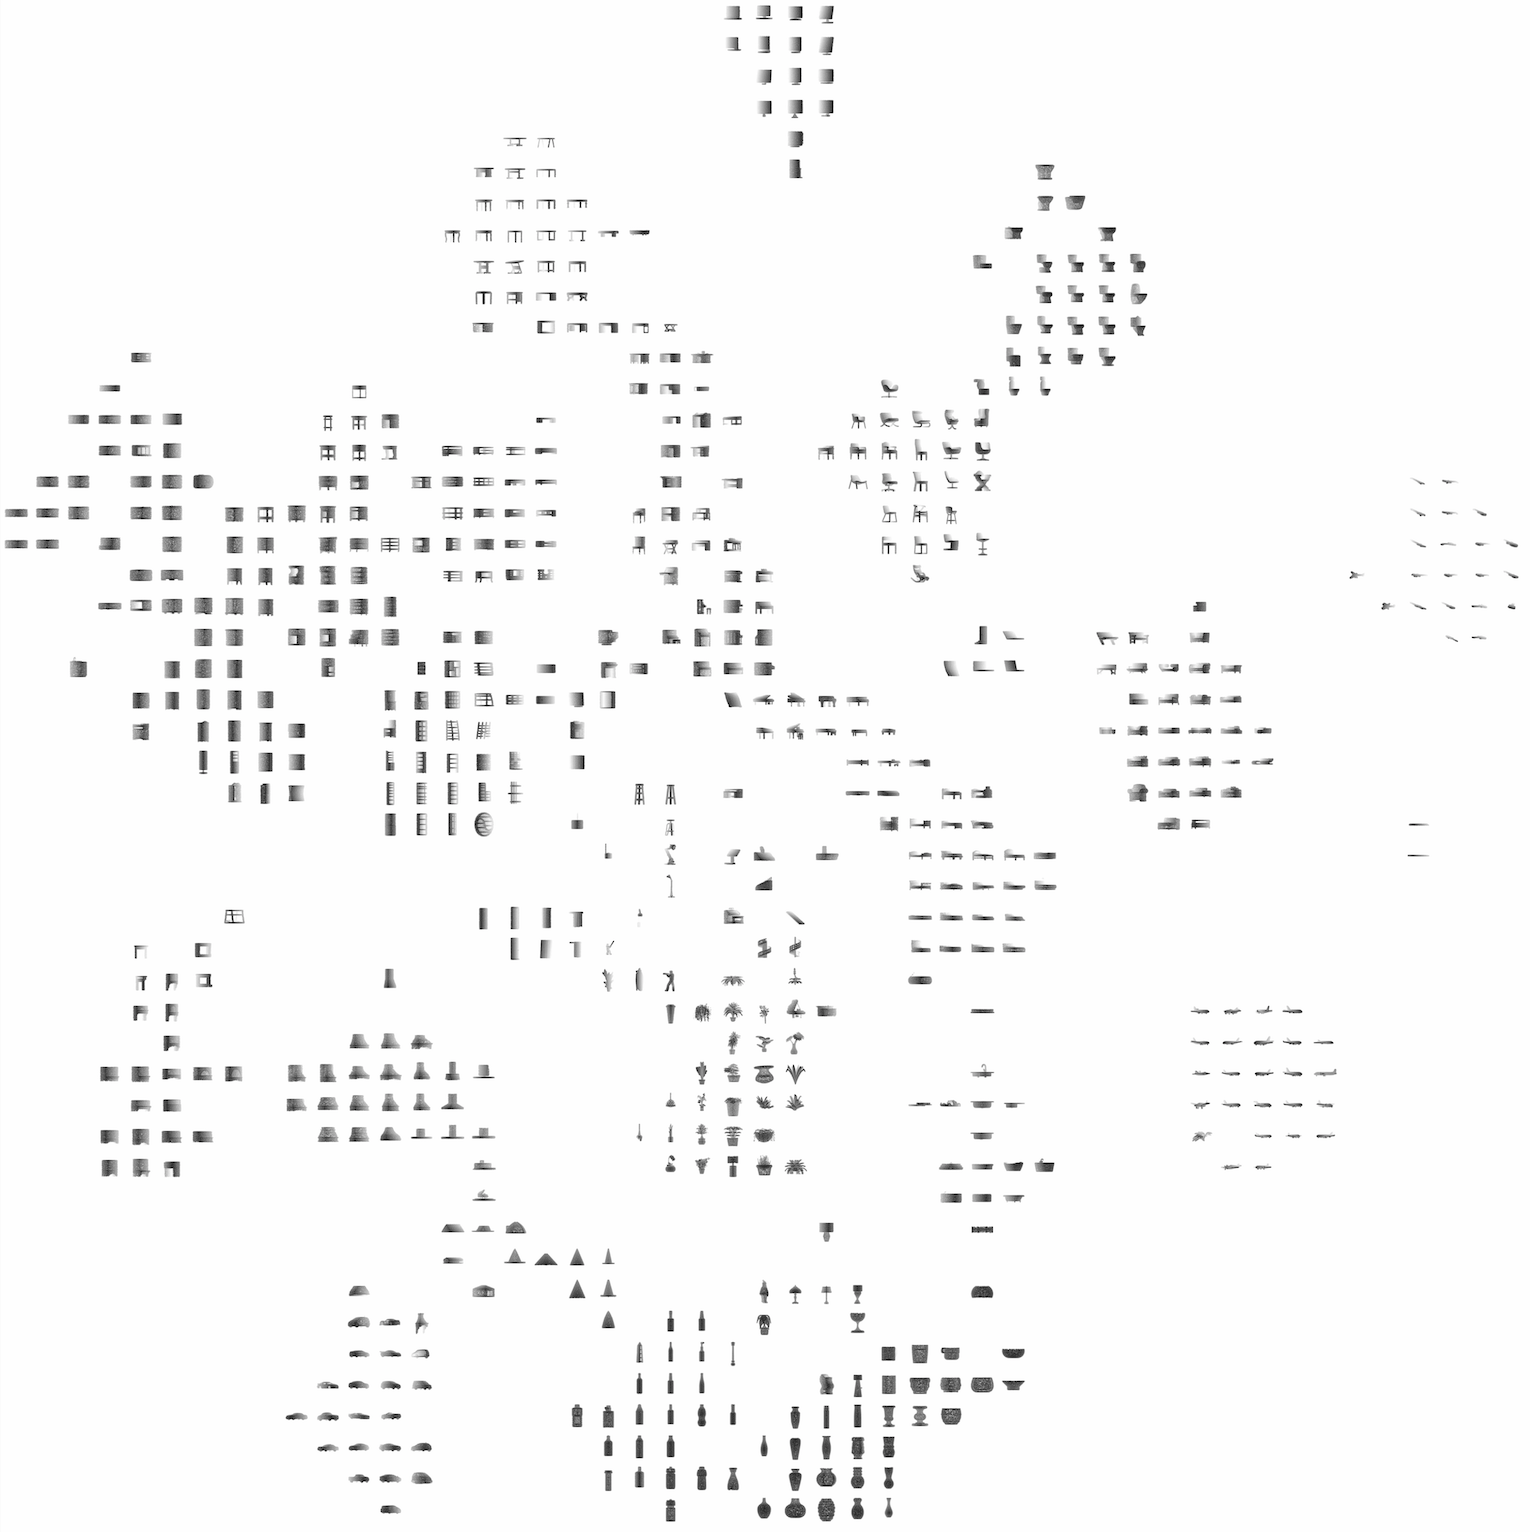
\includegraphics[width=\linewidth]{fig/tsne.png}
\caption{\textbf{所学到的形状全局特征的二维嵌入}我们使用t-SNE技术将学习到的全局形状特征可视化为ModelNet40测试时拆分的形状。}
\label{fig:tsne}
\end{figure*}


\paragraph{分割可视化} 我们在完整的CAD模型和模拟Kinect部分扫描上提供了更多的分割结果。我们还可视化了具有错误分析的失败案例。 图~\ref{fig:part_seg_complete} 和 图~\ref{fig:part_seg_partial} 显示了在完整CAD模型及其模拟Kinect扫描上生成的更多分割结果。 图~\ref{fig:part_seg_failure} 说明了一些失败案例情况。请阅读错误分析的说明。

\begin{figure*}[t!]
\centering
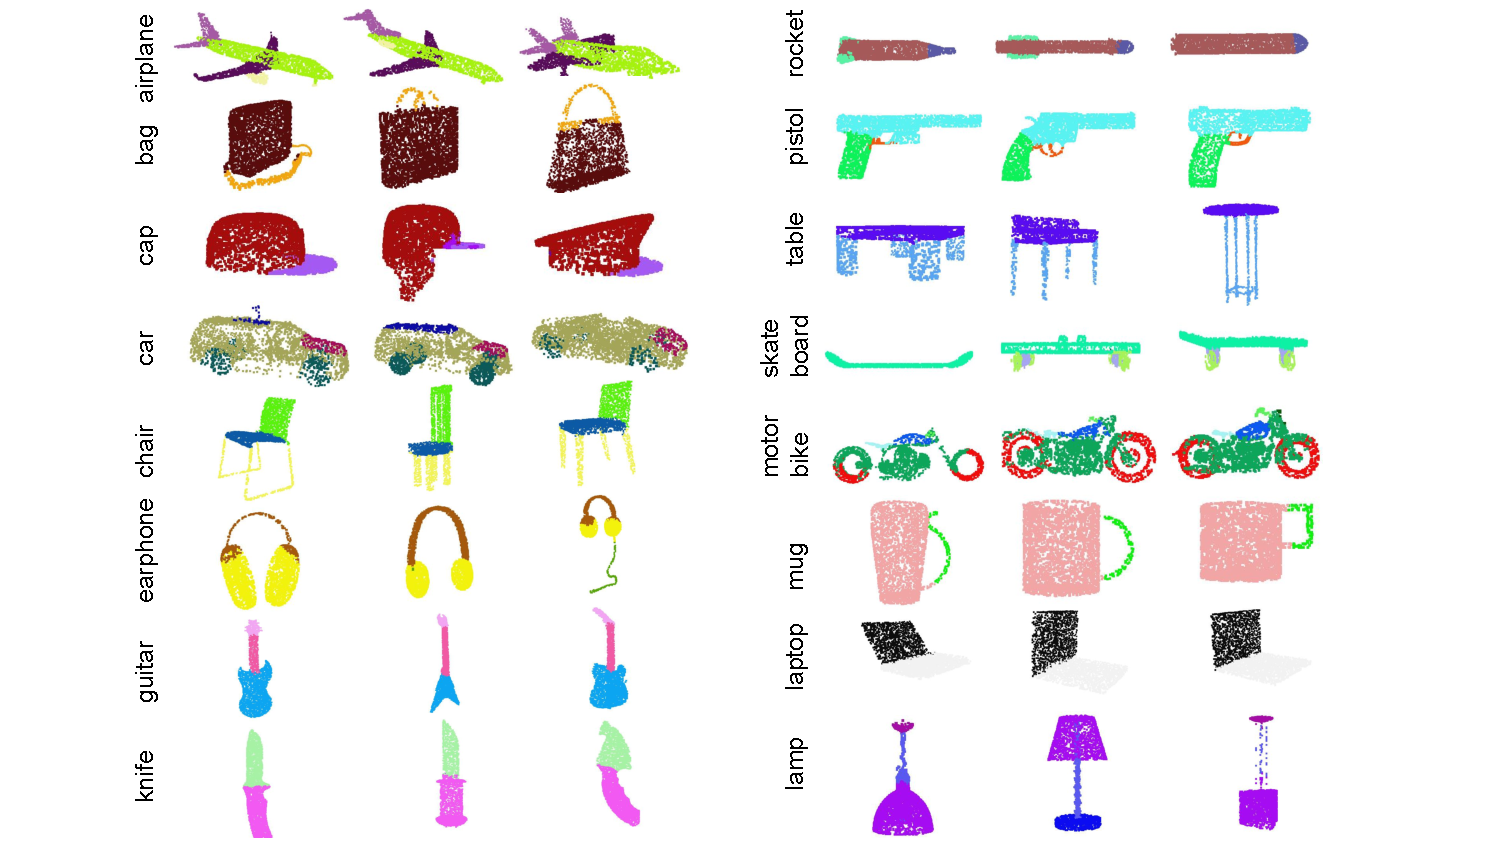
\includegraphics[width=0.82\linewidth]{fig/part_seg_complete.pdf}
\caption{\textbf{PointNet在完整的CAD模型上的分割结果} }
\label{fig:part_seg_complete}
\end{figure*}

\begin{figure*}[t!]
\centering
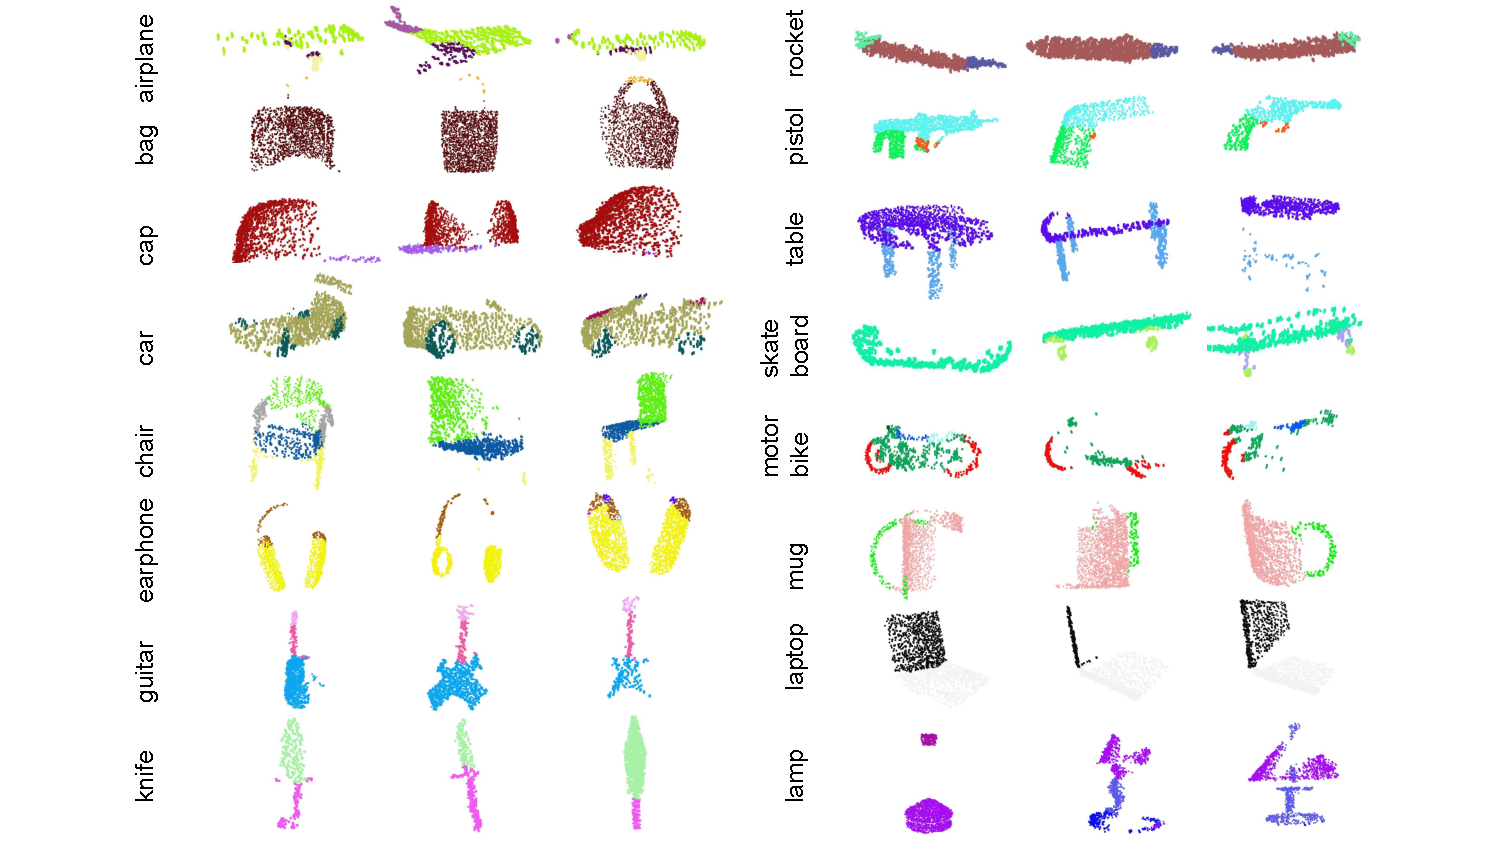
\includegraphics[width=0.82\linewidth]{fig/part_seg_partial.pdf}
\caption{\textbf{PointNet在模拟Kinect扫描上的分割结果} }
\label{fig:part_seg_partial}
\end{figure*}

\begin{figure*}[t!]
\centering
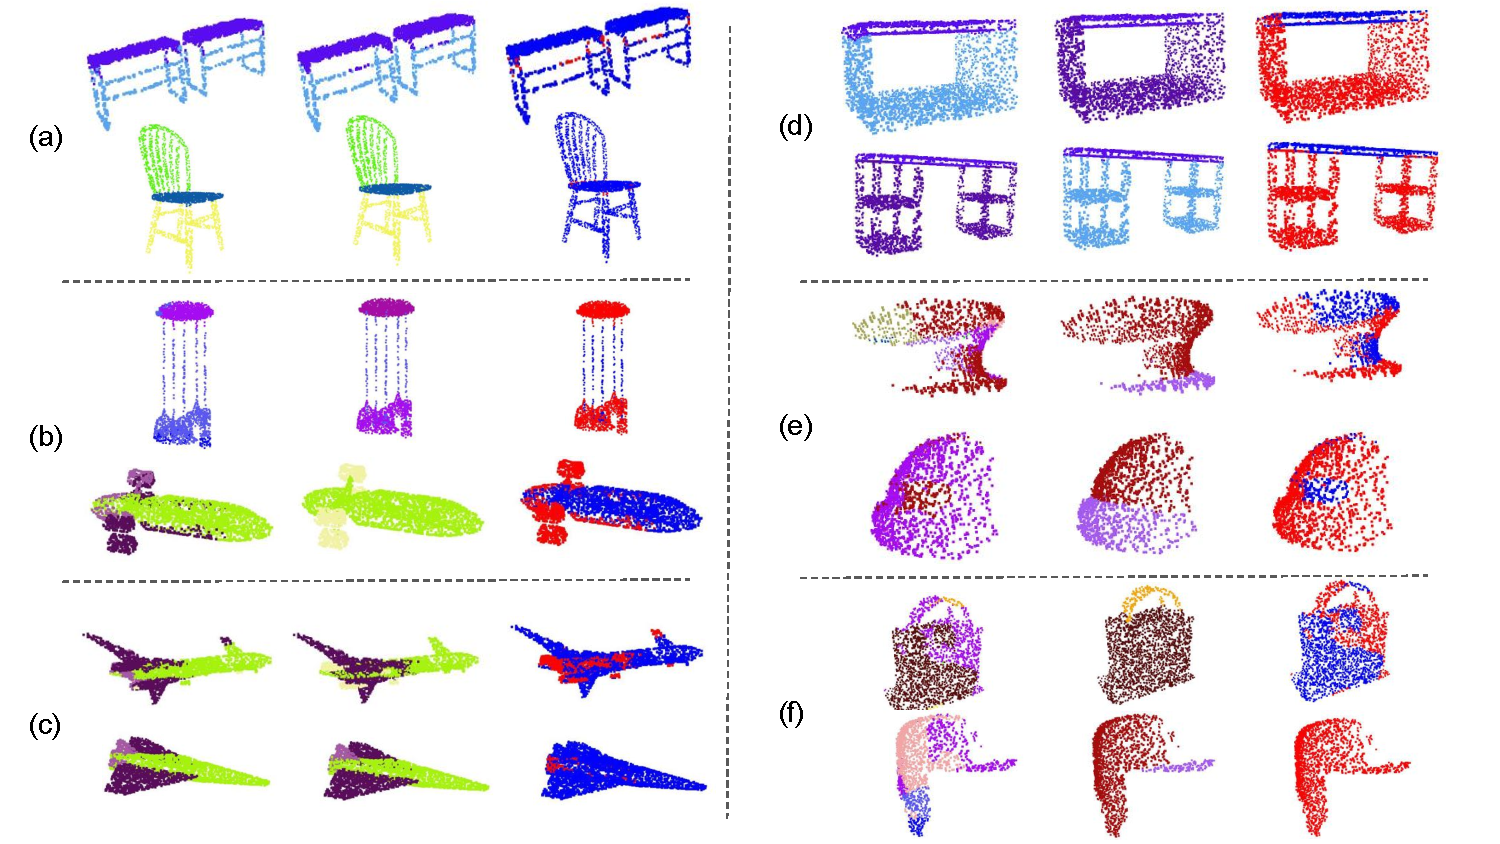
\includegraphics[width=\linewidth]{fig/part_seg_failure.pdf}
\caption{\textbf{PointNet分割失败案例} 在此图中,我们总结了分割应用程序中的六种常见错误。在第一列和第二列中分别给出了预测和真实分割结果,而差异图经计算后显示在第三列。红点对应于给定点云中标记错误的点。(a)说明了最常见的失败案例:边界上的点被错误标记。在示例中,桌椅腿和顶部之间的交叉线附近的点的标签预测不准确。然而,大多数分割算法都存在这个错误。(b)显示了奇怪形状的错误。例如,图中所示的吊灯和飞机在数据集中非常少见。(c)表明小部分可以被附近的大部分覆盖。例如,飞机的喷气发动机(图中黄色)被错误地分类为机身(绿色)或机翼(紫色)。(d)显示了由形状部分固有的模糊性引起的错误。例如,图中两张桌子的两个底部被分类为桌腿和桌脚 (\cite{Yi16}中的\textit{其他}类别),而真实分割则是相反的。(e)显示了由部分扫描的不完整性导致的错误。对于图中的两个帽子,几乎一半的点云都缺失了。(f)显示了当某些目标类别的训练数据太少而无法涵盖足够多样性时产生的失败案例。对于此处显示的两个类别,整个数据集中只有54个袋子和39个帽子。}
\label{fig:part_seg_failure}
\end{figure*}

\paragraph{场景语义解析可视化}
我们在图~\ref{fig:semantic_large} 中给出了语义解析的可视化,其中我们显示了对应两个办公室和一个会议室,用于语义分割和目标检测的输入点云、预测和真实标签。该区域和房间在训练集中是不可见的。


\begin{figure*}
    \centering
    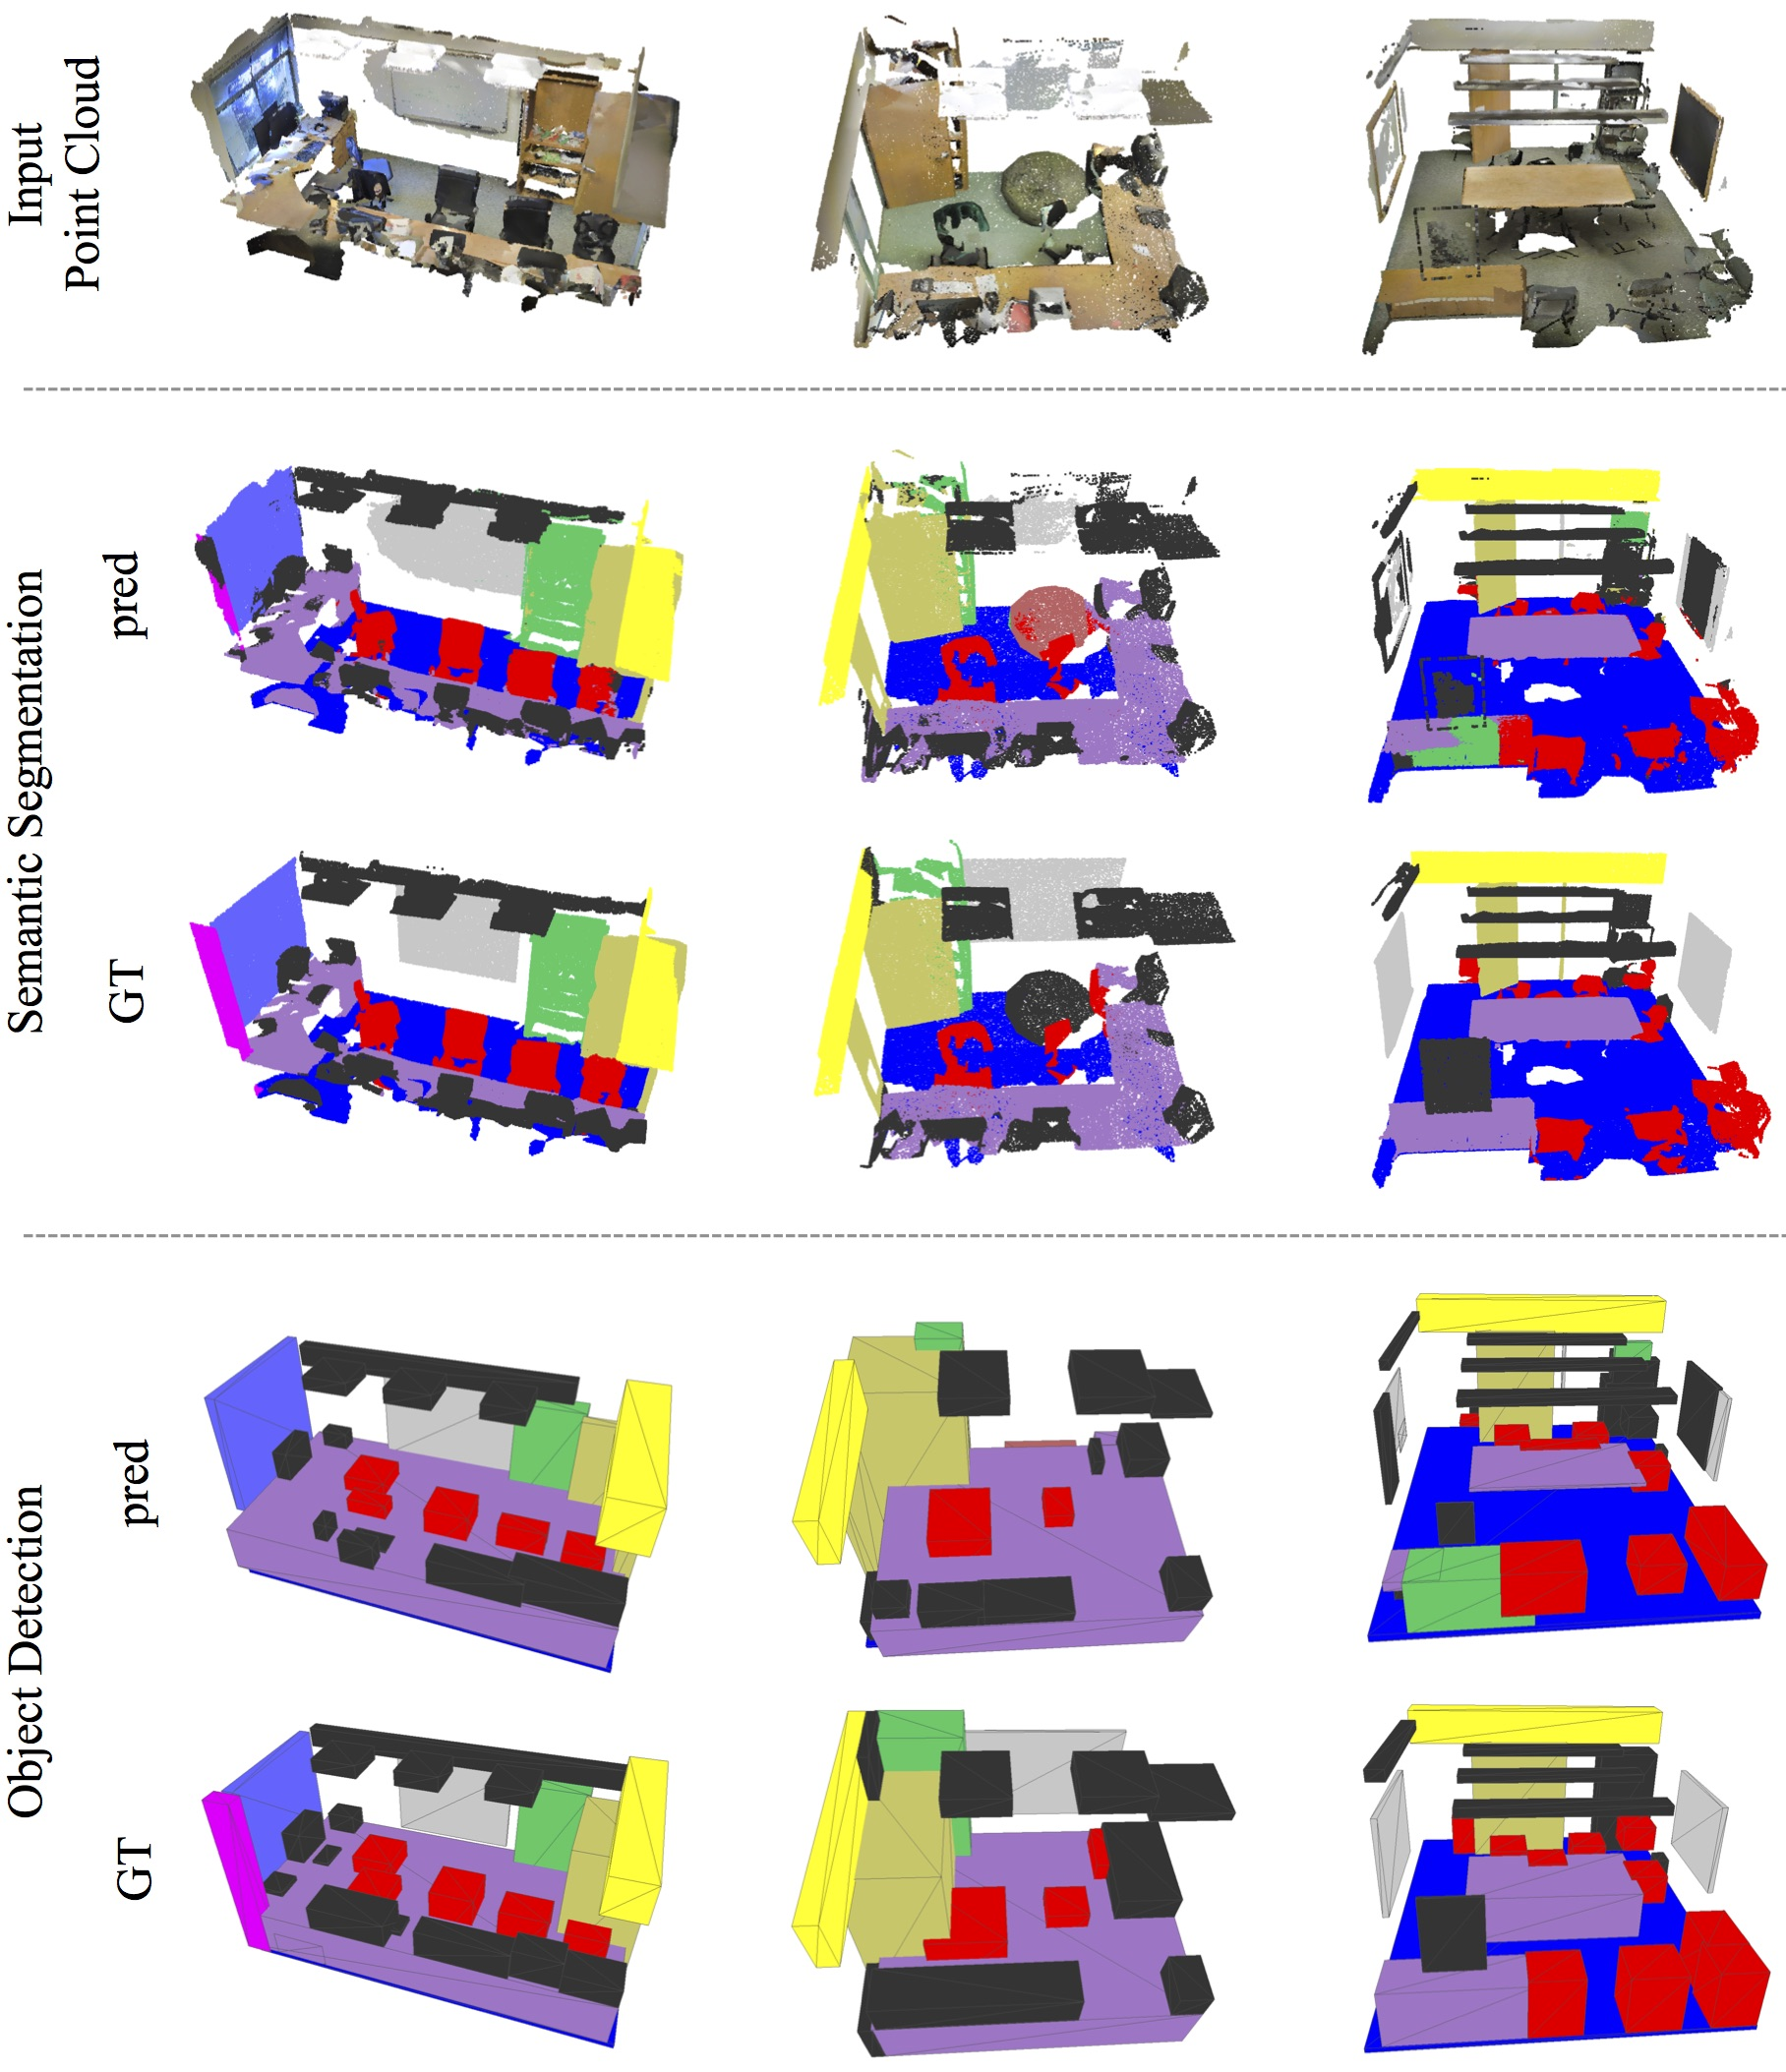
\includegraphics[width=\linewidth]{fig/semantic_large.jpg}
    \caption{\textbf{语义分割和目标检测示例}    第一行是输入点云,为了清晰度,其中墙壁和天花板被隐藏了。第二行和第三行分别是对点的语义分割的预测和真实分割,其中属于不同语义区域的点的颜色不同(椅子为红色,桌子为紫色,沙发为橙色,木板为灰色,书柜为绿色,地板为蓝色,窗户为紫色,横梁为黄色,柱子为洋红色,门为卡其色和杂物为黑色)。最后两行是带有边界框的目标检测,其中预测框来自基于语义分割预测的连接部分。}
    \label{fig:semantic_large}
\end{figure*}

\paragraph{点函数可视化} 我们的分类PointNet为每个点计算 $K$ (我们在此可视化中取 $K=1024$) 维的点特征,并通过最大池化层将所有每点局部特征聚合为单个 $K$维向量,从而形成全局形状描述符。

为了更深入地了解每个已经训练好的点函数 $h$ 所检测的内容。我们在图~\ref{fig:functions} 中可视化了具有较高的点函数值 $f(p_i)$ 的点 $p_i$。该可视化清晰地表明,不同的点函数能够会检测分散在整个空间中的不同区域中形状各异的点。


% \paragraph{Global Feature Visualization} In Fig~\ref{fig:kp_ss_visu}, we visualize more results of the \textit{critical point sets} $\mathcal{C}_S$ and the \textit{upper-bound shapes} $\mathcal{N}_S$ for some sample shapes $S$. The point sets between the two shapes will give exactly the same global shape feature $f(S)$. 

% We can see clearly from Fig~\ref{fig:kp_ss_visu} that the \textit{critical point sets} $\mathcal{C}_S$ summarizes the skeleton of the shape.
% %, or sample a sparse collection of points to describe the geometry of the whole shape.
% The \textit{upper-bound shapes} $\mathcal{N}_S$ illustrates the largest possible point cloud that give the same global shape feature $f(S)$ as the input point cloud $S$. $\mathcal{C}_S$ and $\mathcal{N}_S$ reflect the robustness of PointNet, meaning that losing some non-critical points does not change the global shape signature $f(S)$ at all.

% \begin{figure*}[t!]
% \centering
% \includegraphics[width=0.9\linewidth]{fig/kp_ss_visu2.pdf}
% \includegraphics[width=0.9\linewidth]{fig/kp_ss_visu1.pdf}
% \caption{\textbf{Visualization of critical point sets and upper-bound shapes.} The first row shows the input point clouds $S$. The second and the third rows show the \textit{critical point sets} $\mathcal{C}_S$ and the \textit{upper-bound shapes} $\mathcal{N}_S$ respectively.}
% \label{fig:kp_ss_visu}
% \end{figure*}

% \newpage
% \section{Appendix}
% 令 $\mathcal{X}=\{S: S\subseteq [0,1]\mbox{ and } |S|=n \}$. 

若以下条件满足,则$f:\mathcal{X}\rightarrow \mathbb{R}$ 是一个$\mathcal{X}$上关于赫斯多夫距离$d_H(\cdot, \cdot)$的连续函数

$\forall \epsilon > 0, \exists \delta >0$, 对于任意一个 $S, S'\in\mathcal{X}$, if $d_H(S, S') < \delta$, then $|f(S)-f(S')|< \epsilon$.

我们证明了 $f$ 可以被对称函数和连续函数的复合函数任意逼近

% \begin{theorem}
\begin{customthm}{1}
假设 $f:\mathcal{X}\rightarrow \mathbb{R}$ 是一个关于赫斯多夫距离$d_H(\cdot, \cdot)$的连续集函数。 $\forall \epsilon > 0$, $\exists$ 一个连续函数 $h$ 和一个对称函数 $g(x_1, \dots, x_n)=\gamma \circ \mbox{MAX}$, 其中 $\gamma$ 一个连续函数, $\mbox{MAX}$是一个取 $n$ 个向量最为输入,然后返回一个元素层面上的最大值的最大化向量运算符, 对于任意一个 $S\in\mathcal{X}$,
% Formally, $\forall \epsilon > 0$, $\exists g_{\epsilon}:\underbrace{\R^{K_\epsilon}\times \dots \times \R^{K_\epsilon}}_n\rightarrow \R$ which is a symmetric function and $h_{\epsilon}: \R^3 \rightarrow \R^{K_\epsilon}$ such that 
\begin{align*}
	|f(S) - \gamma(\mbox{MAX}(h(x_1), \ldots, h(x_n)))| < \epsilon
\end{align*}
其中 $x_1, \ldots, x_n$ 是按指定顺序从 $S$ 中提取的元素。
\end{customthm}
%\end{theorem}

\begin{proof}
通过 $f$ 的连续性, 引入 $\delta_{\epsilon}$ 来说明 
$|f(S)-f(S')|<\epsilon$ 对于任意一个 $S, S'\in \mathcal{X} \mbox{ if } d_H(S, S')<\delta_{\epsilon}$. 

定义 $K=\lceil 1/\delta_{\epsilon}\rceil$, 将 $[0,1]$ 均分成 $K$ 个间隔,同时定义辅助函数,将点映射到它所在间隔的左端:
$$\sigma(x)=\frac{\lfloor K x \rfloor}{K}$$
令 $\tilde{S}=\{\sigma(x):x\in S\}$
$$|f(S)-f(\tilde{S})|< \epsilon$$
因为 $d_H(S, \tilde{S})<1/K\le \delta_{\epsilon}$.

令 $h_k(x)=e^{-d(x, [\frac{k-1}{K}, \frac{k}{K}])}$ 为一个轻指示函数,其中 $d(x, I)$ 是点的间隔距离。 令 $\myvec h(x)=[h_1(x); \ldots; h_K(x)]$,  $\myvec h:\mathbb{R}\rightarrow \mathbb{R}^K$. 

令 $v_j(x_1, \ldots, x_n)=\max\{\tilde{h}_j(x_1),\ldots,\tilde{h}_j(x_n)\}$ 代表第$j$-th区间中$S$中点的占比。 令 $\myvec v=[v_1;\ldots; v_K]$, $\myvec v:\underbrace{\mathbb{R}\times \ldots\times \mathbb{R}}_{n}\rightarrow \{0, 1\}^K$ 是一个对称函数, 代表每个区间中$S$中点的占比。

定义 $\tau:\{0, 1\}^K\rightarrow \mathcal{X}$ 为 $\tau(v)=\{\frac{k-1}{K}: v_k\ge 1\}$, 代表占用向量到表示每个占用区间左端集合的映射。 易得:
\begin{align*}
\tau(\myvec v(x_1, \ldots, x_n))\equiv \tilde{S} 
\end{align*}
其中 $x_1, \ldots, x_n$ 是按指定顺序从 $S$ 中提取的元素。

令 $\gamma:\mathbb{R}^K\rightarrow \mathbb{R}$ 为一个连续函数,对于 $v\in\{0, 1\}^K$ 有 $\gamma(\myvec v)=f(\tau(\myvec v))$ 对于 $v\in\{0, 1\}^K$. 则
\begin{align*}
&|\gamma(\myvec v(x_1, \ldots, x_n))-f(S)|\\
=&|f(\tau(\myvec v(x_1, \ldots, x_n)))-f(S)|<\epsilon
\end{align*}

注意 $\gamma(\myvec v(x_1, \ldots, x_n))$ 可以被写成以下形式:
\begin{align*}
\gamma(\myvec v(x_1, \ldots, x_n))=&\gamma(\mbox{MAX}(\myvec h(x_1), \ldots, \myvec h(x_n)))\\
=&(\gamma \circ \mbox{MAX}) (\myvec h(x_1),\ldots,\myvec h(x_n))
\end{align*}
显然 $\gamma \circ \mbox{MAX}$ 是一个对称函数。
% $f(\tau(\myvec v(x_1,\ldots, x_n)))$. Clearly, $\gamma$ is a piece-wise constant function. Due to the universal approximation property of neural networks, 
\end{proof}

接下来给出定理2的证明。
定义 $\myvec u=\underset{x_i\in S}{\mbox{MAX}}\{h(x_i)\}$ 为$f$的子网络,表示$[0,1]^m$上点集到$K$-维向量的映射。以下定理表明输入点集中较少点缺失或者额外微小点扰动不会改变我们网络的输出:
% \begin{theorem}
\begin{customthm}{2}
假设 $\myvec u:\mathcal{X}\rightarrow \mathbb{R}^K$ 其中 $\myvec u=\underset{x_i\in S}{\mbox{MAX}}\{h(x_i)\}$ 且 $f=\gamma \circ \myvec u$. 则, 
\begin{enumerate}[label=(\alph*)]   
    \item $\forall S, \exists~\mathcal{C}_S, \mathcal{N}_S\subseteq \mathcal{X}$,  $f(T)=f(S)$ if  $\mathcal{C}_S\subseteq T\subseteq \mathcal{N}_S$;
    %\item Define the equivalence relation $\sim$ as $S\sim S'$ if $\myvec u(S)=\myvec u(S')$, then $\mathcal{C}_S=\underset{S'\sim S}{\cap} S'$ and $\mathcal{N}_S=\underset{S'\sim S}{\cup} S'$.
    % \item Let $S\sim S'$ if $\myvec u(S)=\myvec u(S')$. $\mathcal{C}_S=\underset{S'\sim S}{\cap} S'$, $\mathcal{N}_S=\underset{S'\sim S}{\cup} S'$.
    \item $|\mathcal{C}_S| \le K$
\end{enumerate}
%\label{thm:thm2}
%     \begin{itemize}            
%     \item Critical points.
%     \\$\mathbb{C}=\{x_i: \myvec u_j(S)=h_j(x_i) \mbox{ for some } 1\le j\le K\}\cap S$
%     \item Free-space points.
%     \\$\mathbb{F}=\{x_i: \myvec u_j(S)<h_j(x_i) \mbox{ for some } 1\le j\le K\}\cap S$
%     \item Non-critical points. 
%     \\$\mathbb{N}=\{x_i: \myvec u_j(S)>h_j(x_i) \mbox{ for some } 1\le j\le K\}\cap S$
% For any $S'$ such that  $\mathbb{C} \subseteq S' \subseteq \mathbb{C}\cup\mathbb{N}$, $\myvec u(S')\equiv \myvec u(S)$; for any $S'$ such that $S'\cap \mathbb{F}\neq \emptyset$, $\myvec u(S')\neq \myvec u(S)$.
%\end{itemize}
\end{customthm}
%\end{theorem}
\begin{proof}
显然, $\forall S\in \mathcal{X}$, $f(S)$ 由$\myvec u(S)$所决定。所以我们只需要证明 
$\forall S, \exists\,\mathcal{C}_S, \mathcal{N}_S\subseteq \mathcal{X}, f(T)=f(S)\,\mbox{if}\,\mathcal{C}_S\subseteq T\subseteq \mathcal{N}_S$. 

对于输出向量$\myvec u$的第$j$维 , 存在至少一个 $x_j \in \mathcal{X}$ 使得 $h_j(x_j)=\myvec u_j$, 其中 $h_j$ 是$h$中第$j$维输出向量。 将 $\mathcal{C}_S$ 作为所有$x_j$ , $j=1,\ldots,K$ 的聚合,则 $\mathcal{C}_S$ 满足上述条件。

因此对于$f$,附加任意额外的点$x$使得$\mathcal{C}_S$的每一维满足$h(x)\le \myvec u(S)$ 而不改变$\myvec u$。从而得出,可以把所有这样点添加到$\mathcal{N}_S$来得到$\mathcal{T}_S$。




\end{proof}

\end{document}

\end{thebibliography}

\bibliographystyle{ieee}
\bibliography{pcl}
}

\newpage

\appendix
\section*{附录}

\section{Overview}
% \begin{itemize}
%     \item \todo{Experiment.} compare pointnet with volumetric cnn and multi-view cnn on corrupted data (missing data). On both classification and segmentation. 
%     \item \todo{Writing.} network details.
%     \item \todo{Dump results.} more applications: normal prediction, correspondence, CAD model retrieval
%     \item (DONE) analysis on bottleneck and number of input points
%     \item (DONE) MNIST
%     \item \todo{Writing. Experiment.} details on object detection system
%     \item \todo{Dump results.} more output visualizations for critical points!! visualization of classification and part segmentation errors. visualization of detection results.
%     \item (DONE) proof of theorems
% \end{itemize}
该文件为主要论文提供了额外的定量结果,技术细节和更多定性的测试示例。 

在 Sec~\ref{sec:cla_robust}中,我们扩展了健壮性测试,以比较不完整输入下的PointNet和VoxNet。 在 Sec~\ref{sec:network}中我们提供了更多有关神经网络架构和训练参数的详细信息, 在 Sec~\ref{sec:detection}中我们描述了场景中的检测流程。Sec~\ref{sec:supp_application} 显示了PointNet的更多应用, 而 Sec~\ref{sec:architecture} 显示了更多的分析实验。 Sec~\ref{sec:proof} 为我们在PointNet上的理论提供了证明。 最后,我们在 Sec~\ref{sec:visu}中显示了更多的可视化结果。


\section{PointNet和VoxNet的比较 (Sec 5.2)}
\label{sec:cla_robust}
我们扩展了第 5.2 节鲁棒性测试中的实验,以比较PointNet和VoxNet~\cite{maturana2015voxnet}(一个用于体积表示的代表性结构)对输入点云中缺失数据的鲁棒性。两个网络都在以 1024 个点作为输入的相同训练测试集上进行训练。对于VoxNet,我们将点云体素化为 $32 \times 32 \times 32$ 的网格,并通过绕上轴随机旋转和抖动来增加训练数据。

在测试时,输入点按一定比例随机丢弃。由于VoxNet对旋转很敏感,它的预测使用来自点云的 12 个视点的平均分数。如图~\ref{fig:compare}所示,我们的PointNet对缺失点更加鲁棒。 当一半的输入点丢失时,VoxNet 的准确率急剧下降,从 $86.3\%$ 到 $46.0\%$,相差 $40.3\%$,而我们的 PointNet 的性能下降只有 $3.7\%$。这可以通过我们 PointNet 的理论分析和解释来解释——它正在学习使用 \textit{critical points} 的集合来总结形状,因此它对缺失数据非常健壮。


\begin{figure}[h!]
    \centering
    \includegraphics[width=0.7\linewidth]{fig/pointnet_vs_voxnet.pdf}
    \caption{\textbf{在不完整输入数据下的PointNet v.s. VoxNet~\cite{maturana2015voxnet} } 指标是 ModelNet40 测试集上的整体分类准确率。请注意,VoxNet 使用 12 个视点平均,而 PointNet 仅使用点云的一个视图。显然 PointNet 对缺失点具有更强的鲁棒性。}
    \label{fig:compare}
\end{figure}

% =============================
% Network details
% =============================
\section{网络架构和训练细节 (Sec 5.1)}
\label{sec:network}
\paragraph{PointNet分类网络}由于论文正文中已经说明了基本的体系结构,因此我们在此处提供有关联合对齐/变换网络和训练参数的更多详细信息。

第一个转换网络是一个mini-PointNet,它直接以未处理的点云为输入,并回归成一个$3\times3$的矩阵。这个网络由一个每个点共享的 $MLP(64,128,1024)$ 网络(输出尺寸分别为64, 128, 1024), 一个点间max pooling和两个全连接层(输出尺寸分别为$512$, $256$)组成。输出矩阵初始值为单位矩阵。除了最后一层,其余所有层都应用了ReLU和Batch Normalization。 第二个变换网络与第一个结构相同,除了输出矩阵尺寸为$64\times64$。输出矩阵也被初始化为单位阵。将正则化损失(权重为0.001)添加到softmax分类损失中,以使矩阵接近正交。

训练时,在估计类别概率前,对最后一层全连接层(维度$256$)应用了keep ratio 为$0.7$的dropout。
Batch Normalization的衰减率从初始的$0.5$逐渐增加到$0.99$。使用adam优化器,初始学习率设置为$0.001$,momentum为$0.9$,batch size为$32$。学习率每迭代20次下降一半。在TensorFlow下用GTX1080 GPU和ModelNet数据集训练,网络需要3-6个小时收敛。

\paragraph{PointNet分割网络}分割网络是PointNet分类网络的一个延伸。对于每个点,将局部点特征(第二个转换网络之后的输出)和全局特征(max pooling的输出)连接在一起。 在分割网络中不使用dropout。训练参数与分类网络相同。

关于形状零件分割的任务,我们对基本分割网络体系结构进行了一些修改 (正文中的图2) 以实现最佳性能。如图~\ref{fig:part_seg_net}所示。 我们添加了一个one-hot向量来显示输入类别并与max pooling的输出连接。 我们还在某些层中增加了神经元个数,并添加了skip links以收集不同层中的局部点特征,并将它们连接起来以形成点特征输入到分割网络中。

\begin{figure}
\centering
\includegraphics[width=\linewidth]{fig/part_seg_net.pdf}
\caption{\textbf{零件分割的网络架构} T1和T2是输入点和特征的对齐/变换网络。FC是在每个点上操作的全连接层。MLP是每一点上的多层感知器。One-hot是一个大小为16的向量,表示输入形状的类别。}
\label{fig:part_seg_net}
\end{figure}

尽管 \cite{Wu2014248} 和 \cite{Yi16} ]独立地处理每个对象类别, 但由于缺少某些类别的训练数据 (第一行显示了数据集中所有类别的形状总数), 我们训练了跨类别的PointNet(但是使用one-hot向量来指示类别).为了进行公平比较,在测试这两个模型时,我们只预测给定特定对象类别的部分标签。

对于语义学分割任务,应用的是与论文主体中相同的基本网络结构,如图2。

使用ShapeNet part 数据集训练需要大约6-12小时,使用Stanford semantic parsing数据集训练大概需要半天。

\paragraph{基准3D CNN分割网络}
在ShapeNet零件分割实验中,我们将建议的分割版本PointNet与两种传统方法以及3D体积CNN网络基准进行了比较。 在图~\ref{fig:voxnet}中, 我们展示了我们使用的基准3D体积CNN网络。 我们将众所周知的3D CNN架构,例如VoxNet \cite{maturana2015voxnet} 和 3DShapeNets \cite{wu20153d} 推广到完全卷积的3D CNN分割网络。

%In the CAD model part segmentation experiment, we compare our proposed segmentation version PointNet to two traditional methods based on shape local features and inter-shape correspondence, as well as a 3D volumetric CNN network as baseline methods. Our PointNet method is a data-driven deep learning method. The comparison between traditional methods to data-driven methods are inherently hard since data-driven methods require more training data than traditional methods. Though we try to test all the methods on the same ShapeNet train/validation/test split, we still think it is crucial to compare our proposed learning-based PointNet with another deep learning method. In Fig.~\ref{fig:voxnet}, we show the baseline 3D volumetric CNN network we use. We generalize the well-known 3D CNN architectures, such as VoxNet \cite{maturana2015voxnet} and 3D ShapeNet \cite{wu20153d} that are invented for classification task, to a 3D CNN segmentation network.

\begin{figure}[t!]
\centering
\includegraphics[width=\linewidth]{fig/voxnet.pdf}
\caption{\textbf{基准3D CNN分割网络.} 该网络是完全卷积化的,并且可以预测每个体素的部分分数}
\label{fig:voxnet}
\end{figure}
对于给定的点云,我们首先将其转换为具有$32 \times 32 \times 32$分辨率的占用网格的体积表示形式。然后,依次使用五个具有32个输出通道和步长为1的3D卷积核来提取特征。每个体素的感受野为19。 %In order to do the final per-pixel label prediction, we choose to keep the size of the feature maps to $32 \times 32 \times 32$ by allowing zero-padding. Zero-padding is reasonable since there are no occupancy for those padded voxels.
最后,将大小为$1\times 1\times 1$的3D卷积序列附加到计算出的特征图上,以预测每个体素的分割标签。除最后一层外,所有层均使用ReLU和Batch Normalization。该网络是跨类别训练的,但是,为了与给出对象类别的其他基准方法进行比较,我们仅考虑给定对象类别中的输出得分。

\section{Details on Detection Pipeline (Sec 5.1)}
\label{sec:detection}
我们基于语义分割结果和我们的对象分类 PointNet 构建了一个简单的 3D 对象检测系统。

我们使用带有分割分数的连接组件来获取场景中的对象提议。从场景中的一个随机点开始,我们找到它的预测标签,并使用 BFS 搜索附近具有相同标签的点,搜索半径为 $0.2$ 米。如果结果集群有超过 200 个点(假设 1m x 1m 区域中有 4096 个点样本),则集群的边界框被标记为一个对象提议。对于每个提议的对象,它的检测分数计算为该类别的平均点分数。在评估之前,面积/体积极小的提案被裁剪。对于桌子、椅子和沙发,边界框会延伸到地板,以防腿与座椅/表面分开。

我们观察到,在某些房间(例如礼堂)中,许多物体(例如椅子)彼此靠近,其中连接的组件无法正确地分割出单个的物体。因此,我们利用我们的分类网络并使用滑动形状方法来缓解椅子类的问题。我们为每个类别训练一个二元分类网络,并使用分类器进行滑动窗口检测。结果框通过非最大抑制进行裁剪。将来自连接组件和滑动形状的建议框组合起来进行最终评估。

在 图~\ref{fig:pr_curve} 中,我们展示了目标检测的准确率-召回率曲线。 我们训练了六个模型,其中每个模型都在五个区域进行训练并在左侧区域进行测试。在测试阶段,每个模型都在它从未见过的区域进行测试。将所有六个区域的测试结果汇总以生成 PR 曲线。
 
 \begin{figure}
 \includegraphics[width=0.8\linewidth]{fig/pr_curve.png}
 \centering
 \caption{\textbf{用于 3D 点云中对象检测的准确率-召回率曲线。} 我们在所有的六个区域上对四个类别进行了评估:桌子、椅子、沙发和木板。 IoU 阈值在体积上表现为 0.5 。}
 \label{fig:pr_curve}
 \end{figure}
 
% =============================
% More Applications
% =============================
\section{更多应用 (Sec 5.1)}
\label{sec:supp_application}
\paragraph{从点云中检索模型} 我们的 PointNet 为每个给定的输入点云学习全局形状特征。我们期望几何相似的形状具有相似的全局特征。在本节中,我们将在形状检索应用程序上测试我们的猜想。更具体地说,对于由 ModelNet 划分的测试集中每个给定查询形状,我们计算其由我们的分类 PointNet 给出的全局签名(分数预测层之前的层的输出),并通过最近邻搜索在划分的训练集中检索相似的形状。结果如图~\ref{fig:retrieval}所示。

\begin{figure}[h]
    \centering
    \includegraphics[width=\linewidth]{fig/retrieval.pdf}
    \caption{\textbf{从点云中检索模型。} 对于每个给定的点云,我们从 ModelNet 划分的测试集中检索前 5 个相似的形状。 从上到下,我们展示了椅子、植物、床头柜和浴缸查询的示例。错误类别的检索结果用红色框标记。}
    \label{fig:retrieval}
\end{figure}

\paragraph{形状对应}
%Since our PointNet learns many per-point functions at the first stage and then aggregates the computed per-point features together using a max-pooling to compute the global shape feature. Thus, there is an inherent correspondence between every coordinate of the global features for a pair of shapes. 

在本节中,我们展示了 PointNet 学习的点特征可以潜在地用于计算形状对应。 给定两个形状,我们通过匹配激活全局特征中相同维度的点对来计算它们的 \textit{critical point sets} $C_S$ 之间的对应关系。Fig~\ref{fig:chair_corr} 和 Fig~\ref{fig:table_corr} 显示了检测到的两个相似椅子和桌子之间的形状对应关系。

\begin{figure}[h]
    \centering
    \includegraphics[width=\linewidth]{fig/chair_corr.png}
    \caption{\textbf{两个椅子之间的形状对应。} 为了可视化的清晰性,我们只展示了 20 个随机挑选的映射对。}
    \label{fig:chair_corr}
\end{figure}

\begin{figure}[h]
    \centering
    \includegraphics[width=\linewidth]{fig/table_corr.png}
    \caption{\textbf{两张桌子之间的形状对应。} 为了可视化的清晰性,我们只展示了 20 个随机挑选的映射对。}
    \label{fig:table_corr}
\end{figure}


% =============================
% More Architecture Analysis
% =============================
\section{更多结构分析 (Sec 5.2)}
\label{sec:architecture}
% \paragraph{Volumetric Reconstruction} To validate proof under Thm2 saying that in the worst case our network will degrade to learn a volumetric respentation for the 3D shape? 

\paragraph{瓶颈维度和输入点数量的有效性}

根据第一个输入层的大小和输入点云的数量,我们的模型的表现会有所变化,接下来我们将阐释其变化。 从图 ~\ref{fig:net_param} 中我们可以看出,随着我们提高点的数量,性能变得越来越好。在大约 1000 个点时,达到饱和。最大的层尺寸同样起了重要作用,让我们将层大小从 64 增大到 1024 之后,表现提升了 $2-4\%$。这说明我们需要足够多的,覆盖整个三维空间的点特征函数来分辨不同的形状。



% \paragraph{Effects of Bottleneck Dimension and Number of Input Points}
% Here we show our model's performance change with regard to the size of the first max layer output as well as the number of input points. In Fig~\ref{fig:net_param} we see that performance grows as we increase the number of points however it saturates at around 1K points. The max layer size plays an important role, increasing the layer size from 64 to 1024 results in a $2-4\%$ performance gain. It indicates that we need enough point feature functions to cover the 3D space in order to discriminate different shapes.

值得一提的是,即便有 64 个点作为了输入(从网络上采样的点中最远的点),我们的网络仍然能够取得令人满意的效果。

% It's worth notice that even with 64 points as input (obtained from furthest point sampling on meshes), our network can achieve decent performance.

\begin{figure}[h]
    \centering
    \includegraphics[width=0.8\linewidth]{fig/bottleneck.pdf}
    \caption{\textbf{瓶颈尺寸和输入点数量的效果} 该指标为 ModelNet40 上的总体的分类准确度。}
    \label{fig:net_param}
\end{figure}

\paragraph{MNIST 数字分类} 在我们关注 3D 点云的学习的同时,我们在用我们的网络在 2D 点云上做了实验,即像素集。

% \paragraph{MNIST Digit Classification}
% While we focus on 3D point cloud learning, a sanity check experiment is to apply our network on a 2D point clouds - pixel sets.

为了将一个 MNIST 图像转换成一个 2D 点云,我们设置了阈值像素值,将所有值大于 128 的像素(用图像中的 $(x,y)$ 坐标表示)加入到集合中。我们使用了一个大小为 256 的集合大小。如果集合中有多于 256 个像素,我们就从中随机地抽样;如果集合中的元素少于 256 个,我们便用集合中存在的点来做填充(由于我们的最大化操作,使用哪一个点来填充并不会影响结果)。

% To convert an MNIST image into a 2D point set we threshold pixel values and add the pixel (represented as a point with $(x,y)$ coordinate in the image) with values larger than 128 to the set. We use a set size of 256. If there are more than 256 pixels int he set, we randomly sub-sample it; if there are less, we pad the set with the one of the pixels in the set (due to our max operation, which point to use for the padding will not affect outcome).

如表 ~\ref{tab:mnist} 所示,我们将其和若干个基准线进行比较(包括将输入图像作为有序向量的多层感知机、将输入图像作为一个从 (0,0) 像素到 (27,27) 像素的循环神经网络、以及一个简易的卷积神经网络)。虽然其中表现最好的模型仍然是一个仔细调试过的卷积神经网络(达到了低于 $0.3\%$ 的错误率),但 PointNet 的表现在二维点集上的表现已经符合预期。

% As seen in Table~\ref{tab:mnist}, we compare with a few baselines including multi-layer perceptron that considers input image as an ordered vector, a RNN that consider input as sequence from pixel (0,0) to pixel (27,27), and a vanilla version CNN. While the best performing model on MNIST is still well engineered CNNs (achieving less than $0.3\%$ error rate), it's interesting to see that our PointNet model can achieve reasonable performance by considering image as a 2D point set.

% vanila CNN: https://www.microsoft.com/en-us/research/publication/best-practices-for-convolutional-neural-networks-applied-to-visual-document-analysis/

\begin{table}[h!]
    \centering
    \begin{tabular}[width=\linewidth]{l|c|c}
    \hline
    ~                      & 输入 & 错误率 (\%) \\ \hline
    多层感知机~\cite{simard2003best} & vector & 1.60  \\
    LeNet5~\cite{lecun1998gradient}                 & image & 0.80 \\ \hline
    我们的 PointNet          & point set & 0.78 \\ \hline
    \end{tabular}
    \caption{\textbf{MNIST 分类结果} 我们将我们的模型和其他简单的深度学习结构进行比对,从而说明我们的模型在二维点云上的表现仍然符合预期。
    % We compare with vanilla versions of other deep architectures to show that our network based on point sets input is achieving reasonable performance on this traditional task.
    }
    \label{tab:mnist}
\end{table}


\paragraph{法线预测}
在分割版本的 PointNet 中,为了为局部的点提供上下文信息,局部的点特征与全局的点特征被拼接在了一起。但这种拼接方式不能保证模型学习到上下文。在该实验中,我们通过展示我们的分割网络具备预测点法线(一个由某个点的邻居所决定的局部几何特征)的能力,来验证我们的设计。

% \paragraph{Normal Estimation}
% In segmentation version of PointNet, local point features and global feature are concatenated in order to provide context to local points. However, it's unclear whether the context is learnt through this concatenation. In this experiment, we validate our design by showing that our segmentation network can be trained to predict point normals, a local geometric property that is determined by a point's neighborhood.

%Our proposed PointNet learns 1024 per-point functions and uses a max-pooling operation to aggregate the per-point features into the global shape feature. Then for classification task, we push this learnt global shape signature to the subsequent classifier. The jump for per-point feature (extremely local) to the shape feature (extremely global) seems fine. However, for segmentation task, one may wonder if the local context entails crucial information to determine the local fine-grained segmentation details. Even though in our segmentation version PointNet we concatenate the learn global shape signature and the per-point local features together to do the label predictions, it is still unclear if such combination can capture the necessary local information around each point. 

我们用一种监督学习的方式修改并训练了我们的分割 PointNet 来回归到真正的点法线。我们仅仅改变了分割 PointNet 的最后一层,使其为每一个点预测法向量。对于损失函数,我们使用了余弦距离的绝对值。

% We train a modified version of our segmentation PointNet in a supervised manner to regress to the ground-truth point normals. We just change the last layer of our segmentation PointNet to predict normal vector for each point. We use absolute value of cosine distance as loss.

图 ~\ref{fig:normal_recon} 对比了我们的 PointNet 法线预测结果(左)和从网格中计算出来的真正的法线(右)。从图中可以看到,我们得到了一个合理的法线重建结果。在一些区域,我们的预测结果甚至比真正的法线(通常包括一些翻转了的法线方向)更加平滑和连续。

% Fig.~\ref{fig:normal_recon} compares our PointNet normal prediction results (the left columns) to the ground-truth normals computed from the mesh (the right columns). We observe a reasonable normal reconstruction. Our predictions are more smooth and continuous than the ground-truth which includes flipped normal directions in some region.
%Having the ability to correctly predict the point normal, one of the local geometric features that require the combination of the information of a point and its neighbors, shows our PointNet has the potential to capture the local information via simply combining the per-point feature and the aggregated global feature.

\begin{figure}[t!]
\centering
\includegraphics[width=0.9\linewidth]{fig/normal_recon2.pdf}
\caption{\textbf{PointNet 法线重建结果。} 改图展示了在一个示例点云中所有点的法线重建结果与从网格中计算出来的真正的法线结果。}
\label{fig:normal_recon}
\end{figure}


\paragraph{分割健壮性} 如 5.2 和 ~\ref{sec:cla_robust} 讨论,由于全局的形状特征是从一些 \textit{关键点} 中提取出来的,我们的点云对于数据干扰和点的缺失并不敏感。在这一部分中,我们展示了我们的模型在面对分割任务时,仍然保持着健壮性。每一个点的标签是根据两部分来预测的:各个点的特征的结合,与模型学习到的全局形状特征。在图 ~\ref{fig:seg_robust} 中,我们展示了给定输入点云 $S$ (左)的分割结果、\textit{关键点集} $\mathcal{C}_S$ (中)和 \textit{上界形状} $\mathcal{N}_S$。

% \paragraph{Segmentation Robustness} As discussed in Sec 5.2 and Sec~\ref{sec:cla_robust}, our PointNet is less sensitive to data corruption and missing points for classification tasks since the global shape feature is extracted from a collection of \textit{critical points} from the given input point cloud. In this section, we show that the robustness holds for segmentation tasks too. The per-point part labels are predicted based on the combination of per-point features and the learnt global shape feature. In Fig~\ref{fig:seg_robust}, we illustrate the segmentation results for the given input point clouds $S$ (the left-most column), the \textit{critical point sets} $\mathcal{C}_S$ (the middle column) and the \textit{upper-bound shapes} $\mathcal{N}_S$.

%One may observe that the segmentation results for the entire shape family containing all the shapes transiting between $\mathcal{C}_S$ and $\mathcal{N}_S$ are consistent, meaning that \textbf{losing some points that are not \textit{critical} does not affect the segmentation result}.

\begin{figure}[t!]
\centering
\includegraphics[width=0.9\linewidth]{fig/seg_robust.pdf}
\caption{\textbf{分割结果的一致性} 我们用图例说明一些样例物体点云的\textit{关键点集} $\mathcal{C}_S$和\textit{上界形状} $\mathcal{N}_S$ 的分割结果。 可以得出从$\mathcal{C}_S$ 到 $\mathcal{N}_S$ 的形状簇拥有共同的分割结果。}
\label{fig:seg_robust}
\end{figure}

% \begin{comment}

在 5.2 \textit{三维物体零件分割}中,我们将我们提出的 PointNet 模型应用在了 CAD 模型的语义零件分割上。我们的分割 PointNet(如图 2 \textit{分割网络})在完整的 ShapeNet 网络上达到了最优的效果。意料之中的,我们的模型在局部数据(如:模拟的 Kinect 扫描结果)中也表现的很好。由于真实世界中的扫描通常因为遮挡问题而变得十分不完整,模型在面对局部输入时的健壮性非常重要,是评估其实际应用价值的关键。表 ~\ref{tab:segmentation_partial} 概括了在面对完整的和局部的数据时,我们的 PointNet 与作为基准线的三维卷积神经网络方法得出的效果。

% In Sec 5.2 \textit{3D Object Part Segmentation}, we apply our proposed PointNet on segmenting the CAD models into semantic parts. While our segmentation PointNet (illustrated in Fig. 2, \textit{Segmentation Network}) achieves the state-of-the-art result on complete ShapeNet shapes, it performs reasonably well on partial data (e.g. simulated Kinect scans) as well. Since most real world scans are very partial due to occlusions, a model's robustness to partial input is key to evaluate its value in practice. Table~\ref{tab:segmentation_partial} summarizes the performance of our PointNet and the proposed baseline 3D CNN method when being applied to complete and partial data.


\begin{table}[h!]
    \small
    \centering
    \begin{tabular}[width=\linewidth]{l|cccc}
    \hline
    ~ & 完整输入 & 局部输入 \\ \hline
    3D CNN & 75.3 & 69.7 \\ \hline
    Ours PointNet & \textbf{80.6} & \textbf{75.3}  \\ \hline
    \end{tabular}
    \caption{\textbf{局部扫描的分割结果} 衡量指标为所有形状的 mIoU。在完整数据上训练我们的点网络时,我们进行了旋转增强,以便与从多个角度生成的模拟Kinect扫描进行公平的比较。两个网络分别在完整数据和部分数据上进行训练,然后在不同的子测试集上进行了测试。}
    \label{tab:segmentation_partial}
\end{table}

% \begin{table}[h!]
%     \small
%     \centering
%     \begin{tabular}[width=\linewidth]{l|cccc}
%     \hline
%     ~ & 完整输入 & 局部输入 \\ \hline
%     3D CNN & 75.3 & 69.7 \\ \hline
%     Ours PointNet & \textbf{80.6} & \textbf{75.3}  \\ \hline
%     \end{tabular}
%     \caption{\textbf{Segmentation results on partial scans.} Metric is mean IoU across all shapes. We perform rotation augmentation when training our PointNet on complete data to fairly compare with the simulated Kinect scans, that are generated from multiple perspective. Both networks are trained respectively on the complete data and the partial data and then tested on the testing splits.}
%     \label{tab:segmentation_partial}
% \end{table}

% \end{comment}

\paragraph{网络面对未知形状分类的通用性}
在图 \ref{fig:unseen} 中,我们可视化了 \textit{关键点集} 和 \textit{上界形状} 在面对来自从未出现在 ModelNet 或 ShapeNet 中的未知分类(脸部、马、兔子、茶壶)的新性状。结果表明,我们的模型学习到的各个点的函数是具备通用性的。然而,由于我们主要使用具备大量平面结构的人造物品来训练模型,重建出来上界形状同样也包含了更多的平面表面。

% In Fig~\ref{fig:unseen}, we visualize the \textit{critical point sets} and the \textit{upper-bound shapes} for new shapes from unseen categories (face, house, rabbit, teapot) that are not present in ModelNet or ShapeNet. It shows that the learnt per-point functions are generalizable. However, since we train mostly on man-made objects with lots of planar structures, the reconstructed upper-bound shape in novel categories also contain more planar surfaces. 
 


% \paragraph{Network Generalizability to Unseen Shape Categories}
% %As discussed in the previous sections, our proposed PointNet learns several useful per-point functions and computes the global shape signature by max pooling all the point features.
% %In Sec 5.3, we visualize the learnt per-point functions and observe that they work in the way to detect if some points intersect with some specific regions. And, by aggregating the learnt per-point features, PointNet selects some \textit{critical points} and produces the global shape feature by summarizing the activation values of them.
% In Fig~\ref{fig:unseen}, we visualize the \textit{critical point sets} and the \textit{upper-bound shapes} for new shapes from unseen categories (face, house, rabbit, teapot) that are not present in ModelNet or ShapeNet. It shows that the learnt per-point functions are generalizable. However, since we train mostly on man-made objects with lots of planar structures, the reconstructed upper-bound shape in novel categories also contain more planar surfaces. 
 
\begin{figure}[t!]
\centering
\includegraphics[width=\linewidth]{fig/unseen.pdf}
\caption{\textbf{未知物体的关键点集和上界形状} 我们可视化了茶壶,兔子,手,人体的 \textit{关键点集} 和 \textit{上界形状}。 通过这些不在ModelNet和ShapeNet数据集的物体来测试PointNet学习到的点函数的通用性。图中用颜色编码反应深度信息。}
\label{fig:unseen}
\end{figure}

\section{定理证明 (Sec 4.3)}
\label{sec:proof}
令 $\mathcal{X}=\{S: S\subseteq [0,1]\mbox{ and } |S|=n \}$. 

若以下条件满足,则$f:\mathcal{X}\rightarrow \mathbb{R}$ 是一个$\mathcal{X}$上关于赫斯多夫距离$d_H(\cdot, \cdot)$的连续函数

$\forall \epsilon > 0, \exists \delta >0$, 对于任意一个 $S, S'\in\mathcal{X}$, if $d_H(S, S') < \delta$, then $|f(S)-f(S')|< \epsilon$.

我们证明了 $f$ 可以被对称函数和连续函数的复合函数任意逼近

% \begin{theorem}
\begin{customthm}{1}
假设 $f:\mathcal{X}\rightarrow \mathbb{R}$ 是一个关于赫斯多夫距离$d_H(\cdot, \cdot)$的连续集函数。 $\forall \epsilon > 0$, $\exists$ 一个连续函数 $h$ 和一个对称函数 $g(x_1, \dots, x_n)=\gamma \circ \mbox{MAX}$, 其中 $\gamma$ 一个连续函数, $\mbox{MAX}$是一个取 $n$ 个向量最为输入,然后返回一个元素层面上的最大值的最大化向量运算符, 对于任意一个 $S\in\mathcal{X}$,
% Formally, $\forall \epsilon > 0$, $\exists g_{\epsilon}:\underbrace{\R^{K_\epsilon}\times \dots \times \R^{K_\epsilon}}_n\rightarrow \R$ which is a symmetric function and $h_{\epsilon}: \R^3 \rightarrow \R^{K_\epsilon}$ such that 
\begin{align*}
	|f(S) - \gamma(\mbox{MAX}(h(x_1), \ldots, h(x_n)))| < \epsilon
\end{align*}
其中 $x_1, \ldots, x_n$ 是按指定顺序从 $S$ 中提取的元素。
\end{customthm}
%\end{theorem}

\begin{proof}
通过 $f$ 的连续性, 引入 $\delta_{\epsilon}$ 来说明 
$|f(S)-f(S')|<\epsilon$ 对于任意一个 $S, S'\in \mathcal{X} \mbox{ if } d_H(S, S')<\delta_{\epsilon}$. 

定义 $K=\lceil 1/\delta_{\epsilon}\rceil$, 将 $[0,1]$ 均分成 $K$ 个间隔,同时定义辅助函数,将点映射到它所在间隔的左端:
$$\sigma(x)=\frac{\lfloor K x \rfloor}{K}$$
令 $\tilde{S}=\{\sigma(x):x\in S\}$
$$|f(S)-f(\tilde{S})|< \epsilon$$
因为 $d_H(S, \tilde{S})<1/K\le \delta_{\epsilon}$.

令 $h_k(x)=e^{-d(x, [\frac{k-1}{K}, \frac{k}{K}])}$ 为一个轻指示函数,其中 $d(x, I)$ 是点的间隔距离。 令 $\myvec h(x)=[h_1(x); \ldots; h_K(x)]$,  $\myvec h:\mathbb{R}\rightarrow \mathbb{R}^K$. 

令 $v_j(x_1, \ldots, x_n)=\max\{\tilde{h}_j(x_1),\ldots,\tilde{h}_j(x_n)\}$ 代表第$j$-th区间中$S$中点的占比。 令 $\myvec v=[v_1;\ldots; v_K]$, $\myvec v:\underbrace{\mathbb{R}\times \ldots\times \mathbb{R}}_{n}\rightarrow \{0, 1\}^K$ 是一个对称函数, 代表每个区间中$S$中点的占比。

定义 $\tau:\{0, 1\}^K\rightarrow \mathcal{X}$ 为 $\tau(v)=\{\frac{k-1}{K}: v_k\ge 1\}$, 代表占用向量到表示每个占用区间左端集合的映射。 易得:
\begin{align*}
\tau(\myvec v(x_1, \ldots, x_n))\equiv \tilde{S} 
\end{align*}
其中 $x_1, \ldots, x_n$ 是按指定顺序从 $S$ 中提取的元素。

令 $\gamma:\mathbb{R}^K\rightarrow \mathbb{R}$ 为一个连续函数,对于 $v\in\{0, 1\}^K$ 有 $\gamma(\myvec v)=f(\tau(\myvec v))$ 对于 $v\in\{0, 1\}^K$. 则
\begin{align*}
&|\gamma(\myvec v(x_1, \ldots, x_n))-f(S)|\\
=&|f(\tau(\myvec v(x_1, \ldots, x_n)))-f(S)|<\epsilon
\end{align*}

注意 $\gamma(\myvec v(x_1, \ldots, x_n))$ 可以被写成以下形式:
\begin{align*}
\gamma(\myvec v(x_1, \ldots, x_n))=&\gamma(\mbox{MAX}(\myvec h(x_1), \ldots, \myvec h(x_n)))\\
=&(\gamma \circ \mbox{MAX}) (\myvec h(x_1),\ldots,\myvec h(x_n))
\end{align*}
显然 $\gamma \circ \mbox{MAX}$ 是一个对称函数。
% $f(\tau(\myvec v(x_1,\ldots, x_n)))$. Clearly, $\gamma$ is a piece-wise constant function. Due to the universal approximation property of neural networks, 
\end{proof}

接下来给出定理2的证明。
定义 $\myvec u=\underset{x_i\in S}{\mbox{MAX}}\{h(x_i)\}$ 为$f$的子网络,表示$[0,1]^m$上点集到$K$-维向量的映射。以下定理表明输入点集中较少点缺失或者额外微小点扰动不会改变我们网络的输出:
% \begin{theorem}
\begin{customthm}{2}
假设 $\myvec u:\mathcal{X}\rightarrow \mathbb{R}^K$ 其中 $\myvec u=\underset{x_i\in S}{\mbox{MAX}}\{h(x_i)\}$ 且 $f=\gamma \circ \myvec u$. 则, 
\begin{enumerate}[label=(\alph*)]   
    \item $\forall S, \exists~\mathcal{C}_S, \mathcal{N}_S\subseteq \mathcal{X}$,  $f(T)=f(S)$ if  $\mathcal{C}_S\subseteq T\subseteq \mathcal{N}_S$;
    %\item Define the equivalence relation $\sim$ as $S\sim S'$ if $\myvec u(S)=\myvec u(S')$, then $\mathcal{C}_S=\underset{S'\sim S}{\cap} S'$ and $\mathcal{N}_S=\underset{S'\sim S}{\cup} S'$.
    % \item Let $S\sim S'$ if $\myvec u(S)=\myvec u(S')$. $\mathcal{C}_S=\underset{S'\sim S}{\cap} S'$, $\mathcal{N}_S=\underset{S'\sim S}{\cup} S'$.
    \item $|\mathcal{C}_S| \le K$
\end{enumerate}
%\label{thm:thm2}
%     \begin{itemize}            
%     \item Critical points.
%     \\$\mathbb{C}=\{x_i: \myvec u_j(S)=h_j(x_i) \mbox{ for some } 1\le j\le K\}\cap S$
%     \item Free-space points.
%     \\$\mathbb{F}=\{x_i: \myvec u_j(S)<h_j(x_i) \mbox{ for some } 1\le j\le K\}\cap S$
%     \item Non-critical points. 
%     \\$\mathbb{N}=\{x_i: \myvec u_j(S)>h_j(x_i) \mbox{ for some } 1\le j\le K\}\cap S$
% For any $S'$ such that  $\mathbb{C} \subseteq S' \subseteq \mathbb{C}\cup\mathbb{N}$, $\myvec u(S')\equiv \myvec u(S)$; for any $S'$ such that $S'\cap \mathbb{F}\neq \emptyset$, $\myvec u(S')\neq \myvec u(S)$.
%\end{itemize}
\end{customthm}
%\end{theorem}
\begin{proof}
显然, $\forall S\in \mathcal{X}$, $f(S)$ 由$\myvec u(S)$所决定。所以我们只需要证明 
$\forall S, \exists\,\mathcal{C}_S, \mathcal{N}_S\subseteq \mathcal{X}, f(T)=f(S)\,\mbox{if}\,\mathcal{C}_S\subseteq T\subseteq \mathcal{N}_S$. 

对于输出向量$\myvec u$的第$j$维 , 存在至少一个 $x_j \in \mathcal{X}$ 使得 $h_j(x_j)=\myvec u_j$, 其中 $h_j$ 是$h$中第$j$维输出向量。 将 $\mathcal{C}_S$ 作为所有$x_j$ , $j=1,\ldots,K$ 的聚合,则 $\mathcal{C}_S$ 满足上述条件。

因此对于$f$,附加任意额外的点$x$使得$\mathcal{C}_S$的每一维满足$h(x)\le \myvec u(S)$ 而不改变$\myvec u$。从而得出,可以把所有这样点添加到$\mathcal{N}_S$来得到$\mathcal{T}_S$。




\end{proof}


\begin{figure}[h!]
    \centering
    \includegraphics[width=0.7\linewidth]{fig/kernels.pdf}
    \caption{\textbf{点函数可视化} 对于每个点函数$h$,计算位于原点的边长为2的立方体中每个点$p$的$h(p)$值 , 该区域覆盖了训练PointNet时输入数据规范化的单位球区域。 在这幅图中, 我们可视化所有$h(p)>0.5$的点$p$,函数值用体素亮度表示。 我们随机选取15个点函数并可视化其活跃区域。}
    \label{fig:functions}
\end{figure}

\section{更多的可视化}
\label{sec:visu}
\paragraph{分类可视化}
%In this section, we investigate the classification version PointNet, visualize the shape global feature space via 2D embedding and provide some error analysis on the failure cases.

我们使用t-SNE\cite{maaten2008visualizing}把从我们的分类PointNet中得到的点云全局结果(1024-dim)降维嵌入到2D空间中。图~\ref{fig:tsne}显示了ModelNet40用于测试的分割形状的嵌入空间。相似的形状根据它们的语义类别分别聚集到一起。

\begin{figure*}[t!]
\centering
\includegraphics[width=\linewidth]{fig/tsne.png}
\caption{\textbf{所学到的形状全局特征的二维嵌入}我们使用t-SNE技术将学习到的全局形状特征可视化为ModelNet40测试时拆分的形状。}
\label{fig:tsne}
\end{figure*}


\paragraph{分割可视化} 我们在完整的CAD模型和模拟Kinect部分扫描上提供了更多的分割结果。我们还可视化了具有错误分析的失败案例。 图~\ref{fig:part_seg_complete} 和 图~\ref{fig:part_seg_partial} 显示了在完整CAD模型及其模拟Kinect扫描上生成的更多分割结果。 图~\ref{fig:part_seg_failure} 说明了一些失败案例情况。请阅读错误分析的说明。

\begin{figure*}[t!]
\centering
\includegraphics[width=0.82\linewidth]{fig/part_seg_complete.pdf}
\caption{\textbf{PointNet在完整的CAD模型上的分割结果} }
\label{fig:part_seg_complete}
\end{figure*}

\begin{figure*}[t!]
\centering
\includegraphics[width=0.82\linewidth]{fig/part_seg_partial.pdf}
\caption{\textbf{PointNet在模拟Kinect扫描上的分割结果} }
\label{fig:part_seg_partial}
\end{figure*}

\begin{figure*}[t!]
\centering
\includegraphics[width=\linewidth]{fig/part_seg_failure.pdf}
\caption{\textbf{PointNet分割失败案例} 在此图中,我们总结了分割应用程序中的六种常见错误。在第一列和第二列中分别给出了预测和真实分割结果,而差异图经计算后显示在第三列。红点对应于给定点云中标记错误的点。(a)说明了最常见的失败案例:边界上的点被错误标记。在示例中,桌椅腿和顶部之间的交叉线附近的点的标签预测不准确。然而,大多数分割算法都存在这个错误。(b)显示了奇怪形状的错误。例如,图中所示的吊灯和飞机在数据集中非常少见。(c)表明小部分可以被附近的大部分覆盖。例如,飞机的喷气发动机(图中黄色)被错误地分类为机身(绿色)或机翼(紫色)。(d)显示了由形状部分固有的模糊性引起的错误。例如,图中两张桌子的两个底部被分类为桌腿和桌脚 (\cite{Yi16}中的\textit{其他}类别),而真实分割则是相反的。(e)显示了由部分扫描的不完整性导致的错误。对于图中的两个帽子,几乎一半的点云都缺失了。(f)显示了当某些目标类别的训练数据太少而无法涵盖足够多样性时产生的失败案例。对于此处显示的两个类别,整个数据集中只有54个袋子和39个帽子。}
\label{fig:part_seg_failure}
\end{figure*}

\paragraph{场景语义解析可视化}
我们在图~\ref{fig:semantic_large} 中给出了语义解析的可视化,其中我们显示了对应两个办公室和一个会议室,用于语义分割和目标检测的输入点云、预测和真实标签。该区域和房间在训练集中是不可见的。


\begin{figure*}
    \centering
    \includegraphics[width=\linewidth]{fig/semantic_large.jpg}
    \caption{\textbf{语义分割和目标检测示例}    第一行是输入点云,为了清晰度,其中墙壁和天花板被隐藏了。第二行和第三行分别是对点的语义分割的预测和真实分割,其中属于不同语义区域的点的颜色不同(椅子为红色,桌子为紫色,沙发为橙色,木板为灰色,书柜为绿色,地板为蓝色,窗户为紫色,横梁为黄色,柱子为洋红色,门为卡其色和杂物为黑色)。最后两行是带有边界框的目标检测,其中预测框来自基于语义分割预测的连接部分。}
    \label{fig:semantic_large}
\end{figure*}

\paragraph{点函数可视化} 我们的分类PointNet为每个点计算 $K$ (我们在此可视化中取 $K=1024$) 维的点特征,并通过最大池化层将所有每点局部特征聚合为单个 $K$维向量,从而形成全局形状描述符。

为了更深入地了解每个已经训练好的点函数 $h$ 所检测的内容。我们在图~\ref{fig:functions} 中可视化了具有较高的点函数值 $f(p_i)$ 的点 $p_i$。该可视化清晰地表明,不同的点函数能够会检测分散在整个空间中的不同区域中形状各异的点。


% \paragraph{Global Feature Visualization} In Fig~\ref{fig:kp_ss_visu}, we visualize more results of the \textit{critical point sets} $\mathcal{C}_S$ and the \textit{upper-bound shapes} $\mathcal{N}_S$ for some sample shapes $S$. The point sets between the two shapes will give exactly the same global shape feature $f(S)$. 

% We can see clearly from Fig~\ref{fig:kp_ss_visu} that the \textit{critical point sets} $\mathcal{C}_S$ summarizes the skeleton of the shape.
% %, or sample a sparse collection of points to describe the geometry of the whole shape.
% The \textit{upper-bound shapes} $\mathcal{N}_S$ illustrates the largest possible point cloud that give the same global shape feature $f(S)$ as the input point cloud $S$. $\mathcal{C}_S$ and $\mathcal{N}_S$ reflect the robustness of PointNet, meaning that losing some non-critical points does not change the global shape signature $f(S)$ at all.

% \begin{figure*}[t!]
% \centering
% \includegraphics[width=0.9\linewidth]{fig/kp_ss_visu2.pdf}
% \includegraphics[width=0.9\linewidth]{fig/kp_ss_visu1.pdf}
% \caption{\textbf{Visualization of critical point sets and upper-bound shapes.} The first row shows the input point clouds $S$. The second and the third rows show the \textit{critical point sets} $\mathcal{C}_S$ and the \textit{upper-bound shapes} $\mathcal{N}_S$ respectively.}
% \label{fig:kp_ss_visu}
% \end{figure*}

% \newpage
% \section{Appendix}
% 令 $\mathcal{X}=\{S: S\subseteq [0,1]\mbox{ and } |S|=n \}$. 

若以下条件满足,则$f:\mathcal{X}\rightarrow \mathbb{R}$ 是一个$\mathcal{X}$上关于赫斯多夫距离$d_H(\cdot, \cdot)$的连续函数

$\forall \epsilon > 0, \exists \delta >0$, 对于任意一个 $S, S'\in\mathcal{X}$, if $d_H(S, S') < \delta$, then $|f(S)-f(S')|< \epsilon$.

我们证明了 $f$ 可以被对称函数和连续函数的复合函数任意逼近

% \begin{theorem}
\begin{customthm}{1}
假设 $f:\mathcal{X}\rightarrow \mathbb{R}$ 是一个关于赫斯多夫距离$d_H(\cdot, \cdot)$的连续集函数。 $\forall \epsilon > 0$, $\exists$ 一个连续函数 $h$ 和一个对称函数 $g(x_1, \dots, x_n)=\gamma \circ \mbox{MAX}$, 其中 $\gamma$ 一个连续函数, $\mbox{MAX}$是一个取 $n$ 个向量最为输入,然后返回一个元素层面上的最大值的最大化向量运算符, 对于任意一个 $S\in\mathcal{X}$,
% Formally, $\forall \epsilon > 0$, $\exists g_{\epsilon}:\underbrace{\R^{K_\epsilon}\times \dots \times \R^{K_\epsilon}}_n\rightarrow \R$ which is a symmetric function and $h_{\epsilon}: \R^3 \rightarrow \R^{K_\epsilon}$ such that 
\begin{align*}
	|f(S) - \gamma(\mbox{MAX}(h(x_1), \ldots, h(x_n)))| < \epsilon
\end{align*}
其中 $x_1, \ldots, x_n$ 是按指定顺序从 $S$ 中提取的元素。
\end{customthm}
%\end{theorem}

\begin{proof}
通过 $f$ 的连续性, 引入 $\delta_{\epsilon}$ 来说明 
$|f(S)-f(S')|<\epsilon$ 对于任意一个 $S, S'\in \mathcal{X} \mbox{ if } d_H(S, S')<\delta_{\epsilon}$. 

定义 $K=\lceil 1/\delta_{\epsilon}\rceil$, 将 $[0,1]$ 均分成 $K$ 个间隔,同时定义辅助函数,将点映射到它所在间隔的左端:
$$\sigma(x)=\frac{\lfloor K x \rfloor}{K}$$
令 $\tilde{S}=\{\sigma(x):x\in S\}$
$$|f(S)-f(\tilde{S})|< \epsilon$$
因为 $d_H(S, \tilde{S})<1/K\le \delta_{\epsilon}$.

令 $h_k(x)=e^{-d(x, [\frac{k-1}{K}, \frac{k}{K}])}$ 为一个轻指示函数,其中 $d(x, I)$ 是点的间隔距离。 令 $\myvec h(x)=[h_1(x); \ldots; h_K(x)]$,  $\myvec h:\mathbb{R}\rightarrow \mathbb{R}^K$. 

令 $v_j(x_1, \ldots, x_n)=\max\{\tilde{h}_j(x_1),\ldots,\tilde{h}_j(x_n)\}$ 代表第$j$-th区间中$S$中点的占比。 令 $\myvec v=[v_1;\ldots; v_K]$, $\myvec v:\underbrace{\mathbb{R}\times \ldots\times \mathbb{R}}_{n}\rightarrow \{0, 1\}^K$ 是一个对称函数, 代表每个区间中$S$中点的占比。

定义 $\tau:\{0, 1\}^K\rightarrow \mathcal{X}$ 为 $\tau(v)=\{\frac{k-1}{K}: v_k\ge 1\}$, 代表占用向量到表示每个占用区间左端集合的映射。 易得:
\begin{align*}
\tau(\myvec v(x_1, \ldots, x_n))\equiv \tilde{S} 
\end{align*}
其中 $x_1, \ldots, x_n$ 是按指定顺序从 $S$ 中提取的元素。

令 $\gamma:\mathbb{R}^K\rightarrow \mathbb{R}$ 为一个连续函数,对于 $v\in\{0, 1\}^K$ 有 $\gamma(\myvec v)=f(\tau(\myvec v))$ 对于 $v\in\{0, 1\}^K$. 则
\begin{align*}
&|\gamma(\myvec v(x_1, \ldots, x_n))-f(S)|\\
=&|f(\tau(\myvec v(x_1, \ldots, x_n)))-f(S)|<\epsilon
\end{align*}

注意 $\gamma(\myvec v(x_1, \ldots, x_n))$ 可以被写成以下形式:
\begin{align*}
\gamma(\myvec v(x_1, \ldots, x_n))=&\gamma(\mbox{MAX}(\myvec h(x_1), \ldots, \myvec h(x_n)))\\
=&(\gamma \circ \mbox{MAX}) (\myvec h(x_1),\ldots,\myvec h(x_n))
\end{align*}
显然 $\gamma \circ \mbox{MAX}$ 是一个对称函数。
% $f(\tau(\myvec v(x_1,\ldots, x_n)))$. Clearly, $\gamma$ is a piece-wise constant function. Due to the universal approximation property of neural networks, 
\end{proof}

接下来给出定理2的证明。
定义 $\myvec u=\underset{x_i\in S}{\mbox{MAX}}\{h(x_i)\}$ 为$f$的子网络,表示$[0,1]^m$上点集到$K$-维向量的映射。以下定理表明输入点集中较少点缺失或者额外微小点扰动不会改变我们网络的输出:
% \begin{theorem}
\begin{customthm}{2}
假设 $\myvec u:\mathcal{X}\rightarrow \mathbb{R}^K$ 其中 $\myvec u=\underset{x_i\in S}{\mbox{MAX}}\{h(x_i)\}$ 且 $f=\gamma \circ \myvec u$. 则, 
\begin{enumerate}[label=(\alph*)]   
    \item $\forall S, \exists~\mathcal{C}_S, \mathcal{N}_S\subseteq \mathcal{X}$,  $f(T)=f(S)$ if  $\mathcal{C}_S\subseteq T\subseteq \mathcal{N}_S$;
    %\item Define the equivalence relation $\sim$ as $S\sim S'$ if $\myvec u(S)=\myvec u(S')$, then $\mathcal{C}_S=\underset{S'\sim S}{\cap} S'$ and $\mathcal{N}_S=\underset{S'\sim S}{\cup} S'$.
    % \item Let $S\sim S'$ if $\myvec u(S)=\myvec u(S')$. $\mathcal{C}_S=\underset{S'\sim S}{\cap} S'$, $\mathcal{N}_S=\underset{S'\sim S}{\cup} S'$.
    \item $|\mathcal{C}_S| \le K$
\end{enumerate}
%\label{thm:thm2}
%     \begin{itemize}            
%     \item Critical points.
%     \\$\mathbb{C}=\{x_i: \myvec u_j(S)=h_j(x_i) \mbox{ for some } 1\le j\le K\}\cap S$
%     \item Free-space points.
%     \\$\mathbb{F}=\{x_i: \myvec u_j(S)<h_j(x_i) \mbox{ for some } 1\le j\le K\}\cap S$
%     \item Non-critical points. 
%     \\$\mathbb{N}=\{x_i: \myvec u_j(S)>h_j(x_i) \mbox{ for some } 1\le j\le K\}\cap S$
% For any $S'$ such that  $\mathbb{C} \subseteq S' \subseteq \mathbb{C}\cup\mathbb{N}$, $\myvec u(S')\equiv \myvec u(S)$; for any $S'$ such that $S'\cap \mathbb{F}\neq \emptyset$, $\myvec u(S')\neq \myvec u(S)$.
%\end{itemize}
\end{customthm}
%\end{theorem}
\begin{proof}
显然, $\forall S\in \mathcal{X}$, $f(S)$ 由$\myvec u(S)$所决定。所以我们只需要证明 
$\forall S, \exists\,\mathcal{C}_S, \mathcal{N}_S\subseteq \mathcal{X}, f(T)=f(S)\,\mbox{if}\,\mathcal{C}_S\subseteq T\subseteq \mathcal{N}_S$. 

对于输出向量$\myvec u$的第$j$维 , 存在至少一个 $x_j \in \mathcal{X}$ 使得 $h_j(x_j)=\myvec u_j$, 其中 $h_j$ 是$h$中第$j$维输出向量。 将 $\mathcal{C}_S$ 作为所有$x_j$ , $j=1,\ldots,K$ 的聚合,则 $\mathcal{C}_S$ 满足上述条件。

因此对于$f$,附加任意额外的点$x$使得$\mathcal{C}_S$的每一维满足$h(x)\le \myvec u(S)$ 而不改变$\myvec u$。从而得出,可以把所有这样点添加到$\mathcal{N}_S$来得到$\mathcal{T}_S$。




\end{proof}

\end{document}

\end{thebibliography}

\bibliographystyle{ieee}
\bibliography{pcl}
}

\newpage

\appendix
\section*{附录}

\section{Overview}
% \begin{itemize}
%     \item \todo{Experiment.} compare pointnet with volumetric cnn and multi-view cnn on corrupted data (missing data). On both classification and segmentation. 
%     \item \todo{Writing.} network details.
%     \item \todo{Dump results.} more applications: normal prediction, correspondence, CAD model retrieval
%     \item (DONE) analysis on bottleneck and number of input points
%     \item (DONE) MNIST
%     \item \todo{Writing. Experiment.} details on object detection system
%     \item \todo{Dump results.} more output visualizations for critical points!! visualization of classification and part segmentation errors. visualization of detection results.
%     \item (DONE) proof of theorems
% \end{itemize}
该文件为主要论文提供了额外的定量结果,技术细节和更多定性的测试示例。 

在 Sec~\ref{sec:cla_robust}中,我们扩展了健壮性测试,以比较不完整输入下的PointNet和VoxNet。 在 Sec~\ref{sec:network}中我们提供了更多有关神经网络架构和训练参数的详细信息, 在 Sec~\ref{sec:detection}中我们描述了场景中的检测流程。Sec~\ref{sec:supp_application} 显示了PointNet的更多应用, 而 Sec~\ref{sec:architecture} 显示了更多的分析实验。 Sec~\ref{sec:proof} 为我们在PointNet上的理论提供了证明。 最后,我们在 Sec~\ref{sec:visu}中显示了更多的可视化结果。


\section{PointNet和VoxNet的比较 (Sec 5.2)}
\label{sec:cla_robust}
我们扩展了第 5.2 节鲁棒性测试中的实验,以比较PointNet和VoxNet~\cite{maturana2015voxnet}(一个用于体积表示的代表性结构)对输入点云中缺失数据的鲁棒性。两个网络都在以 1024 个点作为输入的相同训练测试集上进行训练。对于VoxNet,我们将点云体素化为 $32 \times 32 \times 32$ 的网格,并通过绕上轴随机旋转和抖动来增加训练数据。

在测试时,输入点按一定比例随机丢弃。由于VoxNet对旋转很敏感,它的预测使用来自点云的 12 个视点的平均分数。如图~\ref{fig:compare}所示,我们的PointNet对缺失点更加鲁棒。 当一半的输入点丢失时,VoxNet 的准确率急剧下降,从 $86.3\%$ 到 $46.0\%$,相差 $40.3\%$,而我们的 PointNet 的性能下降只有 $3.7\%$。这可以通过我们 PointNet 的理论分析和解释来解释——它正在学习使用 \textit{critical points} 的集合来总结形状,因此它对缺失数据非常健壮。


\begin{figure}[h!]
    \centering
    \includegraphics[width=0.7\linewidth]{fig/pointnet_vs_voxnet.pdf}
    \caption{\textbf{在不完整输入数据下的PointNet v.s. VoxNet~\cite{maturana2015voxnet} } 指标是 ModelNet40 测试集上的整体分类准确率。请注意,VoxNet 使用 12 个视点平均,而 PointNet 仅使用点云的一个视图。显然 PointNet 对缺失点具有更强的鲁棒性。}
    \label{fig:compare}
\end{figure}

% =============================
% Network details
% =============================
\section{网络架构和训练细节 (Sec 5.1)}
\label{sec:network}
\paragraph{PointNet分类网络}由于论文正文中已经说明了基本的体系结构,因此我们在此处提供有关联合对齐/变换网络和训练参数的更多详细信息。

第一个转换网络是一个mini-PointNet,它直接以未处理的点云为输入,并回归成一个$3\times3$的矩阵。这个网络由一个每个点共享的 $MLP(64,128,1024)$ 网络(输出尺寸分别为64, 128, 1024), 一个点间max pooling和两个全连接层(输出尺寸分别为$512$, $256$)组成。输出矩阵初始值为单位矩阵。除了最后一层,其余所有层都应用了ReLU和Batch Normalization。 第二个变换网络与第一个结构相同,除了输出矩阵尺寸为$64\times64$。输出矩阵也被初始化为单位阵。将正则化损失(权重为0.001)添加到softmax分类损失中,以使矩阵接近正交。

训练时,在估计类别概率前,对最后一层全连接层(维度$256$)应用了keep ratio 为$0.7$的dropout。
Batch Normalization的衰减率从初始的$0.5$逐渐增加到$0.99$。使用adam优化器,初始学习率设置为$0.001$,momentum为$0.9$,batch size为$32$。学习率每迭代20次下降一半。在TensorFlow下用GTX1080 GPU和ModelNet数据集训练,网络需要3-6个小时收敛。

\paragraph{PointNet分割网络}分割网络是PointNet分类网络的一个延伸。对于每个点,将局部点特征(第二个转换网络之后的输出)和全局特征(max pooling的输出)连接在一起。 在分割网络中不使用dropout。训练参数与分类网络相同。

关于形状零件分割的任务,我们对基本分割网络体系结构进行了一些修改 (正文中的图2) 以实现最佳性能。如图~\ref{fig:part_seg_net}所示。 我们添加了一个one-hot向量来显示输入类别并与max pooling的输出连接。 我们还在某些层中增加了神经元个数,并添加了skip links以收集不同层中的局部点特征,并将它们连接起来以形成点特征输入到分割网络中。

\begin{figure}
\centering
\includegraphics[width=\linewidth]{fig/part_seg_net.pdf}
\caption{\textbf{零件分割的网络架构} T1和T2是输入点和特征的对齐/变换网络。FC是在每个点上操作的全连接层。MLP是每一点上的多层感知器。One-hot是一个大小为16的向量,表示输入形状的类别。}
\label{fig:part_seg_net}
\end{figure}

尽管 \cite{Wu2014248} 和 \cite{Yi16} ]独立地处理每个对象类别, 但由于缺少某些类别的训练数据 (第一行显示了数据集中所有类别的形状总数), 我们训练了跨类别的PointNet(但是使用one-hot向量来指示类别).为了进行公平比较,在测试这两个模型时,我们只预测给定特定对象类别的部分标签。

对于语义学分割任务,应用的是与论文主体中相同的基本网络结构,如图2。

使用ShapeNet part 数据集训练需要大约6-12小时,使用Stanford semantic parsing数据集训练大概需要半天。

\paragraph{基准3D CNN分割网络}
在ShapeNet零件分割实验中,我们将建议的分割版本PointNet与两种传统方法以及3D体积CNN网络基准进行了比较。 在图~\ref{fig:voxnet}中, 我们展示了我们使用的基准3D体积CNN网络。 我们将众所周知的3D CNN架构,例如VoxNet \cite{maturana2015voxnet} 和 3DShapeNets \cite{wu20153d} 推广到完全卷积的3D CNN分割网络。

%In the CAD model part segmentation experiment, we compare our proposed segmentation version PointNet to two traditional methods based on shape local features and inter-shape correspondence, as well as a 3D volumetric CNN network as baseline methods. Our PointNet method is a data-driven deep learning method. The comparison between traditional methods to data-driven methods are inherently hard since data-driven methods require more training data than traditional methods. Though we try to test all the methods on the same ShapeNet train/validation/test split, we still think it is crucial to compare our proposed learning-based PointNet with another deep learning method. In Fig.~\ref{fig:voxnet}, we show the baseline 3D volumetric CNN network we use. We generalize the well-known 3D CNN architectures, such as VoxNet \cite{maturana2015voxnet} and 3D ShapeNet \cite{wu20153d} that are invented for classification task, to a 3D CNN segmentation network.

\begin{figure}[t!]
\centering
\includegraphics[width=\linewidth]{fig/voxnet.pdf}
\caption{\textbf{基准3D CNN分割网络.} 该网络是完全卷积化的,并且可以预测每个体素的部分分数}
\label{fig:voxnet}
\end{figure}
对于给定的点云,我们首先将其转换为具有$32 \times 32 \times 32$分辨率的占用网格的体积表示形式。然后,依次使用五个具有32个输出通道和步长为1的3D卷积核来提取特征。每个体素的感受野为19。 %In order to do the final per-pixel label prediction, we choose to keep the size of the feature maps to $32 \times 32 \times 32$ by allowing zero-padding. Zero-padding is reasonable since there are no occupancy for those padded voxels.
最后,将大小为$1\times 1\times 1$的3D卷积序列附加到计算出的特征图上,以预测每个体素的分割标签。除最后一层外,所有层均使用ReLU和Batch Normalization。该网络是跨类别训练的,但是,为了与给出对象类别的其他基准方法进行比较,我们仅考虑给定对象类别中的输出得分。

\section{Details on Detection Pipeline (Sec 5.1)}
\label{sec:detection}
我们基于语义分割结果和我们的对象分类 PointNet 构建了一个简单的 3D 对象检测系统。

我们使用带有分割分数的连接组件来获取场景中的对象提议。从场景中的一个随机点开始,我们找到它的预测标签,并使用 BFS 搜索附近具有相同标签的点,搜索半径为 $0.2$ 米。如果结果集群有超过 200 个点(假设 1m x 1m 区域中有 4096 个点样本),则集群的边界框被标记为一个对象提议。对于每个提议的对象,它的检测分数计算为该类别的平均点分数。在评估之前,面积/体积极小的提案被裁剪。对于桌子、椅子和沙发,边界框会延伸到地板,以防腿与座椅/表面分开。

我们观察到,在某些房间(例如礼堂)中,许多物体(例如椅子)彼此靠近,其中连接的组件无法正确地分割出单个的物体。因此,我们利用我们的分类网络并使用滑动形状方法来缓解椅子类的问题。我们为每个类别训练一个二元分类网络,并使用分类器进行滑动窗口检测。结果框通过非最大抑制进行裁剪。将来自连接组件和滑动形状的建议框组合起来进行最终评估。

在 图~\ref{fig:pr_curve} 中,我们展示了目标检测的准确率-召回率曲线。 我们训练了六个模型,其中每个模型都在五个区域进行训练并在左侧区域进行测试。在测试阶段,每个模型都在它从未见过的区域进行测试。将所有六个区域的测试结果汇总以生成 PR 曲线。
 
 \begin{figure}
 \includegraphics[width=0.8\linewidth]{fig/pr_curve.png}
 \centering
 \caption{\textbf{用于 3D 点云中对象检测的准确率-召回率曲线。} 我们在所有的六个区域上对四个类别进行了评估:桌子、椅子、沙发和木板。 IoU 阈值在体积上表现为 0.5 。}
 \label{fig:pr_curve}
 \end{figure}
 
% =============================
% More Applications
% =============================
\section{更多应用 (Sec 5.1)}
\label{sec:supp_application}
\paragraph{从点云中检索模型} 我们的 PointNet 为每个给定的输入点云学习全局形状特征。我们期望几何相似的形状具有相似的全局特征。在本节中,我们将在形状检索应用程序上测试我们的猜想。更具体地说,对于由 ModelNet 划分的测试集中每个给定查询形状,我们计算其由我们的分类 PointNet 给出的全局签名(分数预测层之前的层的输出),并通过最近邻搜索在划分的训练集中检索相似的形状。结果如图~\ref{fig:retrieval}所示。

\begin{figure}[h]
    \centering
    \includegraphics[width=\linewidth]{fig/retrieval.pdf}
    \caption{\textbf{从点云中检索模型。} 对于每个给定的点云,我们从 ModelNet 划分的测试集中检索前 5 个相似的形状。 从上到下,我们展示了椅子、植物、床头柜和浴缸查询的示例。错误类别的检索结果用红色框标记。}
    \label{fig:retrieval}
\end{figure}

\paragraph{形状对应}
%Since our PointNet learns many per-point functions at the first stage and then aggregates the computed per-point features together using a max-pooling to compute the global shape feature. Thus, there is an inherent correspondence between every coordinate of the global features for a pair of shapes. 

在本节中,我们展示了 PointNet 学习的点特征可以潜在地用于计算形状对应。 给定两个形状,我们通过匹配激活全局特征中相同维度的点对来计算它们的 \textit{critical point sets} $C_S$ 之间的对应关系。Fig~\ref{fig:chair_corr} 和 Fig~\ref{fig:table_corr} 显示了检测到的两个相似椅子和桌子之间的形状对应关系。

\begin{figure}[h]
    \centering
    \includegraphics[width=\linewidth]{fig/chair_corr.png}
    \caption{\textbf{两个椅子之间的形状对应。} 为了可视化的清晰性,我们只展示了 20 个随机挑选的映射对。}
    \label{fig:chair_corr}
\end{figure}

\begin{figure}[h]
    \centering
    \includegraphics[width=\linewidth]{fig/table_corr.png}
    \caption{\textbf{两张桌子之间的形状对应。} 为了可视化的清晰性,我们只展示了 20 个随机挑选的映射对。}
    \label{fig:table_corr}
\end{figure}


% =============================
% More Architecture Analysis
% =============================
\section{更多结构分析 (Sec 5.2)}
\label{sec:architecture}
% \paragraph{Volumetric Reconstruction} To validate proof under Thm2 saying that in the worst case our network will degrade to learn a volumetric respentation for the 3D shape? 

\paragraph{瓶颈维度和输入点数量的有效性}

根据第一个输入层的大小和输入点云的数量,我们的模型的表现会有所变化,接下来我们将阐释其变化。 从图 ~\ref{fig:net_param} 中我们可以看出,随着我们提高点的数量,性能变得越来越好。在大约 1000 个点时,达到饱和。最大的层尺寸同样起了重要作用,让我们将层大小从 64 增大到 1024 之后,表现提升了 $2-4\%$。这说明我们需要足够多的,覆盖整个三维空间的点特征函数来分辨不同的形状。



% \paragraph{Effects of Bottleneck Dimension and Number of Input Points}
% Here we show our model's performance change with regard to the size of the first max layer output as well as the number of input points. In Fig~\ref{fig:net_param} we see that performance grows as we increase the number of points however it saturates at around 1K points. The max layer size plays an important role, increasing the layer size from 64 to 1024 results in a $2-4\%$ performance gain. It indicates that we need enough point feature functions to cover the 3D space in order to discriminate different shapes.

值得一提的是,即便有 64 个点作为了输入(从网络上采样的点中最远的点),我们的网络仍然能够取得令人满意的效果。

% It's worth notice that even with 64 points as input (obtained from furthest point sampling on meshes), our network can achieve decent performance.

\begin{figure}[h]
    \centering
    \includegraphics[width=0.8\linewidth]{fig/bottleneck.pdf}
    \caption{\textbf{瓶颈尺寸和输入点数量的效果} 该指标为 ModelNet40 上的总体的分类准确度。}
    \label{fig:net_param}
\end{figure}

\paragraph{MNIST 数字分类} 在我们关注 3D 点云的学习的同时,我们在用我们的网络在 2D 点云上做了实验,即像素集。

% \paragraph{MNIST Digit Classification}
% While we focus on 3D point cloud learning, a sanity check experiment is to apply our network on a 2D point clouds - pixel sets.

为了将一个 MNIST 图像转换成一个 2D 点云,我们设置了阈值像素值,将所有值大于 128 的像素(用图像中的 $(x,y)$ 坐标表示)加入到集合中。我们使用了一个大小为 256 的集合大小。如果集合中有多于 256 个像素,我们就从中随机地抽样;如果集合中的元素少于 256 个,我们便用集合中存在的点来做填充(由于我们的最大化操作,使用哪一个点来填充并不会影响结果)。

% To convert an MNIST image into a 2D point set we threshold pixel values and add the pixel (represented as a point with $(x,y)$ coordinate in the image) with values larger than 128 to the set. We use a set size of 256. If there are more than 256 pixels int he set, we randomly sub-sample it; if there are less, we pad the set with the one of the pixels in the set (due to our max operation, which point to use for the padding will not affect outcome).

如表 ~\ref{tab:mnist} 所示,我们将其和若干个基准线进行比较(包括将输入图像作为有序向量的多层感知机、将输入图像作为一个从 (0,0) 像素到 (27,27) 像素的循环神经网络、以及一个简易的卷积神经网络)。虽然其中表现最好的模型仍然是一个仔细调试过的卷积神经网络(达到了低于 $0.3\%$ 的错误率),但 PointNet 的表现在二维点集上的表现已经符合预期。

% As seen in Table~\ref{tab:mnist}, we compare with a few baselines including multi-layer perceptron that considers input image as an ordered vector, a RNN that consider input as sequence from pixel (0,0) to pixel (27,27), and a vanilla version CNN. While the best performing model on MNIST is still well engineered CNNs (achieving less than $0.3\%$ error rate), it's interesting to see that our PointNet model can achieve reasonable performance by considering image as a 2D point set.

% vanila CNN: https://www.microsoft.com/en-us/research/publication/best-practices-for-convolutional-neural-networks-applied-to-visual-document-analysis/

\begin{table}[h!]
    \centering
    \begin{tabular}[width=\linewidth]{l|c|c}
    \hline
    ~                      & 输入 & 错误率 (\%) \\ \hline
    多层感知机~\cite{simard2003best} & vector & 1.60  \\
    LeNet5~\cite{lecun1998gradient}                 & image & 0.80 \\ \hline
    我们的 PointNet          & point set & 0.78 \\ \hline
    \end{tabular}
    \caption{\textbf{MNIST 分类结果} 我们将我们的模型和其他简单的深度学习结构进行比对,从而说明我们的模型在二维点云上的表现仍然符合预期。
    % We compare with vanilla versions of other deep architectures to show that our network based on point sets input is achieving reasonable performance on this traditional task.
    }
    \label{tab:mnist}
\end{table}


\paragraph{法线预测}
在分割版本的 PointNet 中,为了为局部的点提供上下文信息,局部的点特征与全局的点特征被拼接在了一起。但这种拼接方式不能保证模型学习到上下文。在该实验中,我们通过展示我们的分割网络具备预测点法线(一个由某个点的邻居所决定的局部几何特征)的能力,来验证我们的设计。

% \paragraph{Normal Estimation}
% In segmentation version of PointNet, local point features and global feature are concatenated in order to provide context to local points. However, it's unclear whether the context is learnt through this concatenation. In this experiment, we validate our design by showing that our segmentation network can be trained to predict point normals, a local geometric property that is determined by a point's neighborhood.

%Our proposed PointNet learns 1024 per-point functions and uses a max-pooling operation to aggregate the per-point features into the global shape feature. Then for classification task, we push this learnt global shape signature to the subsequent classifier. The jump for per-point feature (extremely local) to the shape feature (extremely global) seems fine. However, for segmentation task, one may wonder if the local context entails crucial information to determine the local fine-grained segmentation details. Even though in our segmentation version PointNet we concatenate the learn global shape signature and the per-point local features together to do the label predictions, it is still unclear if such combination can capture the necessary local information around each point. 

我们用一种监督学习的方式修改并训练了我们的分割 PointNet 来回归到真正的点法线。我们仅仅改变了分割 PointNet 的最后一层,使其为每一个点预测法向量。对于损失函数,我们使用了余弦距离的绝对值。

% We train a modified version of our segmentation PointNet in a supervised manner to regress to the ground-truth point normals. We just change the last layer of our segmentation PointNet to predict normal vector for each point. We use absolute value of cosine distance as loss.

图 ~\ref{fig:normal_recon} 对比了我们的 PointNet 法线预测结果(左)和从网格中计算出来的真正的法线(右)。从图中可以看到,我们得到了一个合理的法线重建结果。在一些区域,我们的预测结果甚至比真正的法线(通常包括一些翻转了的法线方向)更加平滑和连续。

% Fig.~\ref{fig:normal_recon} compares our PointNet normal prediction results (the left columns) to the ground-truth normals computed from the mesh (the right columns). We observe a reasonable normal reconstruction. Our predictions are more smooth and continuous than the ground-truth which includes flipped normal directions in some region.
%Having the ability to correctly predict the point normal, one of the local geometric features that require the combination of the information of a point and its neighbors, shows our PointNet has the potential to capture the local information via simply combining the per-point feature and the aggregated global feature.

\begin{figure}[t!]
\centering
\includegraphics[width=0.9\linewidth]{fig/normal_recon2.pdf}
\caption{\textbf{PointNet 法线重建结果。} 改图展示了在一个示例点云中所有点的法线重建结果与从网格中计算出来的真正的法线结果。}
\label{fig:normal_recon}
\end{figure}


\paragraph{分割健壮性} 如 5.2 和 ~\ref{sec:cla_robust} 讨论,由于全局的形状特征是从一些 \textit{关键点} 中提取出来的,我们的点云对于数据干扰和点的缺失并不敏感。在这一部分中,我们展示了我们的模型在面对分割任务时,仍然保持着健壮性。每一个点的标签是根据两部分来预测的:各个点的特征的结合,与模型学习到的全局形状特征。在图 ~\ref{fig:seg_robust} 中,我们展示了给定输入点云 $S$ (左)的分割结果、\textit{关键点集} $\mathcal{C}_S$ (中)和 \textit{上界形状} $\mathcal{N}_S$。

% \paragraph{Segmentation Robustness} As discussed in Sec 5.2 and Sec~\ref{sec:cla_robust}, our PointNet is less sensitive to data corruption and missing points for classification tasks since the global shape feature is extracted from a collection of \textit{critical points} from the given input point cloud. In this section, we show that the robustness holds for segmentation tasks too. The per-point part labels are predicted based on the combination of per-point features and the learnt global shape feature. In Fig~\ref{fig:seg_robust}, we illustrate the segmentation results for the given input point clouds $S$ (the left-most column), the \textit{critical point sets} $\mathcal{C}_S$ (the middle column) and the \textit{upper-bound shapes} $\mathcal{N}_S$.

%One may observe that the segmentation results for the entire shape family containing all the shapes transiting between $\mathcal{C}_S$ and $\mathcal{N}_S$ are consistent, meaning that \textbf{losing some points that are not \textit{critical} does not affect the segmentation result}.

\begin{figure}[t!]
\centering
\includegraphics[width=0.9\linewidth]{fig/seg_robust.pdf}
\caption{\textbf{分割结果的一致性} 我们用图例说明一些样例物体点云的\textit{关键点集} $\mathcal{C}_S$和\textit{上界形状} $\mathcal{N}_S$ 的分割结果。 可以得出从$\mathcal{C}_S$ 到 $\mathcal{N}_S$ 的形状簇拥有共同的分割结果。}
\label{fig:seg_robust}
\end{figure}

% \begin{comment}

在 5.2 \textit{三维物体零件分割}中,我们将我们提出的 PointNet 模型应用在了 CAD 模型的语义零件分割上。我们的分割 PointNet(如图 2 \textit{分割网络})在完整的 ShapeNet 网络上达到了最优的效果。意料之中的,我们的模型在局部数据(如:模拟的 Kinect 扫描结果)中也表现的很好。由于真实世界中的扫描通常因为遮挡问题而变得十分不完整,模型在面对局部输入时的健壮性非常重要,是评估其实际应用价值的关键。表 ~\ref{tab:segmentation_partial} 概括了在面对完整的和局部的数据时,我们的 PointNet 与作为基准线的三维卷积神经网络方法得出的效果。

% In Sec 5.2 \textit{3D Object Part Segmentation}, we apply our proposed PointNet on segmenting the CAD models into semantic parts. While our segmentation PointNet (illustrated in Fig. 2, \textit{Segmentation Network}) achieves the state-of-the-art result on complete ShapeNet shapes, it performs reasonably well on partial data (e.g. simulated Kinect scans) as well. Since most real world scans are very partial due to occlusions, a model's robustness to partial input is key to evaluate its value in practice. Table~\ref{tab:segmentation_partial} summarizes the performance of our PointNet and the proposed baseline 3D CNN method when being applied to complete and partial data.


\begin{table}[h!]
    \small
    \centering
    \begin{tabular}[width=\linewidth]{l|cccc}
    \hline
    ~ & 完整输入 & 局部输入 \\ \hline
    3D CNN & 75.3 & 69.7 \\ \hline
    Ours PointNet & \textbf{80.6} & \textbf{75.3}  \\ \hline
    \end{tabular}
    \caption{\textbf{局部扫描的分割结果} 衡量指标为所有形状的 mIoU。在完整数据上训练我们的点网络时,我们进行了旋转增强,以便与从多个角度生成的模拟Kinect扫描进行公平的比较。两个网络分别在完整数据和部分数据上进行训练,然后在不同的子测试集上进行了测试。}
    \label{tab:segmentation_partial}
\end{table}

% \begin{table}[h!]
%     \small
%     \centering
%     \begin{tabular}[width=\linewidth]{l|cccc}
%     \hline
%     ~ & 完整输入 & 局部输入 \\ \hline
%     3D CNN & 75.3 & 69.7 \\ \hline
%     Ours PointNet & \textbf{80.6} & \textbf{75.3}  \\ \hline
%     \end{tabular}
%     \caption{\textbf{Segmentation results on partial scans.} Metric is mean IoU across all shapes. We perform rotation augmentation when training our PointNet on complete data to fairly compare with the simulated Kinect scans, that are generated from multiple perspective. Both networks are trained respectively on the complete data and the partial data and then tested on the testing splits.}
%     \label{tab:segmentation_partial}
% \end{table}

% \end{comment}

\paragraph{网络面对未知形状分类的通用性}
在图 \ref{fig:unseen} 中,我们可视化了 \textit{关键点集} 和 \textit{上界形状} 在面对来自从未出现在 ModelNet 或 ShapeNet 中的未知分类(脸部、马、兔子、茶壶)的新性状。结果表明,我们的模型学习到的各个点的函数是具备通用性的。然而,由于我们主要使用具备大量平面结构的人造物品来训练模型,重建出来上界形状同样也包含了更多的平面表面。

% In Fig~\ref{fig:unseen}, we visualize the \textit{critical point sets} and the \textit{upper-bound shapes} for new shapes from unseen categories (face, house, rabbit, teapot) that are not present in ModelNet or ShapeNet. It shows that the learnt per-point functions are generalizable. However, since we train mostly on man-made objects with lots of planar structures, the reconstructed upper-bound shape in novel categories also contain more planar surfaces. 
 


% \paragraph{Network Generalizability to Unseen Shape Categories}
% %As discussed in the previous sections, our proposed PointNet learns several useful per-point functions and computes the global shape signature by max pooling all the point features.
% %In Sec 5.3, we visualize the learnt per-point functions and observe that they work in the way to detect if some points intersect with some specific regions. And, by aggregating the learnt per-point features, PointNet selects some \textit{critical points} and produces the global shape feature by summarizing the activation values of them.
% In Fig~\ref{fig:unseen}, we visualize the \textit{critical point sets} and the \textit{upper-bound shapes} for new shapes from unseen categories (face, house, rabbit, teapot) that are not present in ModelNet or ShapeNet. It shows that the learnt per-point functions are generalizable. However, since we train mostly on man-made objects with lots of planar structures, the reconstructed upper-bound shape in novel categories also contain more planar surfaces. 
 
\begin{figure}[t!]
\centering
\includegraphics[width=\linewidth]{fig/unseen.pdf}
\caption{\textbf{未知物体的关键点集和上界形状} 我们可视化了茶壶,兔子,手,人体的 \textit{关键点集} 和 \textit{上界形状}。 通过这些不在ModelNet和ShapeNet数据集的物体来测试PointNet学习到的点函数的通用性。图中用颜色编码反应深度信息。}
\label{fig:unseen}
\end{figure}

\section{定理证明 (Sec 4.3)}
\label{sec:proof}
令 $\mathcal{X}=\{S: S\subseteq [0,1]\mbox{ and } |S|=n \}$. 

若以下条件满足,则$f:\mathcal{X}\rightarrow \mathbb{R}$ 是一个$\mathcal{X}$上关于赫斯多夫距离$d_H(\cdot, \cdot)$的连续函数

$\forall \epsilon > 0, \exists \delta >0$, 对于任意一个 $S, S'\in\mathcal{X}$, if $d_H(S, S') < \delta$, then $|f(S)-f(S')|< \epsilon$.

我们证明了 $f$ 可以被对称函数和连续函数的复合函数任意逼近

% \begin{theorem}
\begin{customthm}{1}
假设 $f:\mathcal{X}\rightarrow \mathbb{R}$ 是一个关于赫斯多夫距离$d_H(\cdot, \cdot)$的连续集函数。 $\forall \epsilon > 0$, $\exists$ 一个连续函数 $h$ 和一个对称函数 $g(x_1, \dots, x_n)=\gamma \circ \mbox{MAX}$, 其中 $\gamma$ 一个连续函数, $\mbox{MAX}$是一个取 $n$ 个向量最为输入,然后返回一个元素层面上的最大值的最大化向量运算符, 对于任意一个 $S\in\mathcal{X}$,
% Formally, $\forall \epsilon > 0$, $\exists g_{\epsilon}:\underbrace{\R^{K_\epsilon}\times \dots \times \R^{K_\epsilon}}_n\rightarrow \R$ which is a symmetric function and $h_{\epsilon}: \R^3 \rightarrow \R^{K_\epsilon}$ such that 
\begin{align*}
	|f(S) - \gamma(\mbox{MAX}(h(x_1), \ldots, h(x_n)))| < \epsilon
\end{align*}
其中 $x_1, \ldots, x_n$ 是按指定顺序从 $S$ 中提取的元素。
\end{customthm}
%\end{theorem}

\begin{proof}
通过 $f$ 的连续性, 引入 $\delta_{\epsilon}$ 来说明 
$|f(S)-f(S')|<\epsilon$ 对于任意一个 $S, S'\in \mathcal{X} \mbox{ if } d_H(S, S')<\delta_{\epsilon}$. 

定义 $K=\lceil 1/\delta_{\epsilon}\rceil$, 将 $[0,1]$ 均分成 $K$ 个间隔,同时定义辅助函数,将点映射到它所在间隔的左端:
$$\sigma(x)=\frac{\lfloor K x \rfloor}{K}$$
令 $\tilde{S}=\{\sigma(x):x\in S\}$
$$|f(S)-f(\tilde{S})|< \epsilon$$
因为 $d_H(S, \tilde{S})<1/K\le \delta_{\epsilon}$.

令 $h_k(x)=e^{-d(x, [\frac{k-1}{K}, \frac{k}{K}])}$ 为一个轻指示函数,其中 $d(x, I)$ 是点的间隔距离。 令 $\myvec h(x)=[h_1(x); \ldots; h_K(x)]$,  $\myvec h:\mathbb{R}\rightarrow \mathbb{R}^K$. 

令 $v_j(x_1, \ldots, x_n)=\max\{\tilde{h}_j(x_1),\ldots,\tilde{h}_j(x_n)\}$ 代表第$j$-th区间中$S$中点的占比。 令 $\myvec v=[v_1;\ldots; v_K]$, $\myvec v:\underbrace{\mathbb{R}\times \ldots\times \mathbb{R}}_{n}\rightarrow \{0, 1\}^K$ 是一个对称函数, 代表每个区间中$S$中点的占比。

定义 $\tau:\{0, 1\}^K\rightarrow \mathcal{X}$ 为 $\tau(v)=\{\frac{k-1}{K}: v_k\ge 1\}$, 代表占用向量到表示每个占用区间左端集合的映射。 易得:
\begin{align*}
\tau(\myvec v(x_1, \ldots, x_n))\equiv \tilde{S} 
\end{align*}
其中 $x_1, \ldots, x_n$ 是按指定顺序从 $S$ 中提取的元素。

令 $\gamma:\mathbb{R}^K\rightarrow \mathbb{R}$ 为一个连续函数,对于 $v\in\{0, 1\}^K$ 有 $\gamma(\myvec v)=f(\tau(\myvec v))$ 对于 $v\in\{0, 1\}^K$. 则
\begin{align*}
&|\gamma(\myvec v(x_1, \ldots, x_n))-f(S)|\\
=&|f(\tau(\myvec v(x_1, \ldots, x_n)))-f(S)|<\epsilon
\end{align*}

注意 $\gamma(\myvec v(x_1, \ldots, x_n))$ 可以被写成以下形式:
\begin{align*}
\gamma(\myvec v(x_1, \ldots, x_n))=&\gamma(\mbox{MAX}(\myvec h(x_1), \ldots, \myvec h(x_n)))\\
=&(\gamma \circ \mbox{MAX}) (\myvec h(x_1),\ldots,\myvec h(x_n))
\end{align*}
显然 $\gamma \circ \mbox{MAX}$ 是一个对称函数。
% $f(\tau(\myvec v(x_1,\ldots, x_n)))$. Clearly, $\gamma$ is a piece-wise constant function. Due to the universal approximation property of neural networks, 
\end{proof}

接下来给出定理2的证明。
定义 $\myvec u=\underset{x_i\in S}{\mbox{MAX}}\{h(x_i)\}$ 为$f$的子网络,表示$[0,1]^m$上点集到$K$-维向量的映射。以下定理表明输入点集中较少点缺失或者额外微小点扰动不会改变我们网络的输出:
% \begin{theorem}
\begin{customthm}{2}
假设 $\myvec u:\mathcal{X}\rightarrow \mathbb{R}^K$ 其中 $\myvec u=\underset{x_i\in S}{\mbox{MAX}}\{h(x_i)\}$ 且 $f=\gamma \circ \myvec u$. 则, 
\begin{enumerate}[label=(\alph*)]   
    \item $\forall S, \exists~\mathcal{C}_S, \mathcal{N}_S\subseteq \mathcal{X}$,  $f(T)=f(S)$ if  $\mathcal{C}_S\subseteq T\subseteq \mathcal{N}_S$;
    %\item Define the equivalence relation $\sim$ as $S\sim S'$ if $\myvec u(S)=\myvec u(S')$, then $\mathcal{C}_S=\underset{S'\sim S}{\cap} S'$ and $\mathcal{N}_S=\underset{S'\sim S}{\cup} S'$.
    % \item Let $S\sim S'$ if $\myvec u(S)=\myvec u(S')$. $\mathcal{C}_S=\underset{S'\sim S}{\cap} S'$, $\mathcal{N}_S=\underset{S'\sim S}{\cup} S'$.
    \item $|\mathcal{C}_S| \le K$
\end{enumerate}
%\label{thm:thm2}
%     \begin{itemize}            
%     \item Critical points.
%     \\$\mathbb{C}=\{x_i: \myvec u_j(S)=h_j(x_i) \mbox{ for some } 1\le j\le K\}\cap S$
%     \item Free-space points.
%     \\$\mathbb{F}=\{x_i: \myvec u_j(S)<h_j(x_i) \mbox{ for some } 1\le j\le K\}\cap S$
%     \item Non-critical points. 
%     \\$\mathbb{N}=\{x_i: \myvec u_j(S)>h_j(x_i) \mbox{ for some } 1\le j\le K\}\cap S$
% For any $S'$ such that  $\mathbb{C} \subseteq S' \subseteq \mathbb{C}\cup\mathbb{N}$, $\myvec u(S')\equiv \myvec u(S)$; for any $S'$ such that $S'\cap \mathbb{F}\neq \emptyset$, $\myvec u(S')\neq \myvec u(S)$.
%\end{itemize}
\end{customthm}
%\end{theorem}
\begin{proof}
显然, $\forall S\in \mathcal{X}$, $f(S)$ 由$\myvec u(S)$所决定。所以我们只需要证明 
$\forall S, \exists\,\mathcal{C}_S, \mathcal{N}_S\subseteq \mathcal{X}, f(T)=f(S)\,\mbox{if}\,\mathcal{C}_S\subseteq T\subseteq \mathcal{N}_S$. 

对于输出向量$\myvec u$的第$j$维 , 存在至少一个 $x_j \in \mathcal{X}$ 使得 $h_j(x_j)=\myvec u_j$, 其中 $h_j$ 是$h$中第$j$维输出向量。 将 $\mathcal{C}_S$ 作为所有$x_j$ , $j=1,\ldots,K$ 的聚合,则 $\mathcal{C}_S$ 满足上述条件。

因此对于$f$,附加任意额外的点$x$使得$\mathcal{C}_S$的每一维满足$h(x)\le \myvec u(S)$ 而不改变$\myvec u$。从而得出,可以把所有这样点添加到$\mathcal{N}_S$来得到$\mathcal{T}_S$。




\end{proof}


\begin{figure}[h!]
    \centering
    \includegraphics[width=0.7\linewidth]{fig/kernels.pdf}
    \caption{\textbf{点函数可视化} 对于每个点函数$h$,计算位于原点的边长为2的立方体中每个点$p$的$h(p)$值 , 该区域覆盖了训练PointNet时输入数据规范化的单位球区域。 在这幅图中, 我们可视化所有$h(p)>0.5$的点$p$,函数值用体素亮度表示。 我们随机选取15个点函数并可视化其活跃区域。}
    \label{fig:functions}
\end{figure}

\section{更多的可视化}
\label{sec:visu}
\paragraph{分类可视化}
%In this section, we investigate the classification version PointNet, visualize the shape global feature space via 2D embedding and provide some error analysis on the failure cases.

我们使用t-SNE\cite{maaten2008visualizing}把从我们的分类PointNet中得到的点云全局结果(1024-dim)降维嵌入到2D空间中。图~\ref{fig:tsne}显示了ModelNet40用于测试的分割形状的嵌入空间。相似的形状根据它们的语义类别分别聚集到一起。

\begin{figure*}[t!]
\centering
\includegraphics[width=\linewidth]{fig/tsne.png}
\caption{\textbf{所学到的形状全局特征的二维嵌入}我们使用t-SNE技术将学习到的全局形状特征可视化为ModelNet40测试时拆分的形状。}
\label{fig:tsne}
\end{figure*}


\paragraph{分割可视化} 我们在完整的CAD模型和模拟Kinect部分扫描上提供了更多的分割结果。我们还可视化了具有错误分析的失败案例。 图~\ref{fig:part_seg_complete} 和 图~\ref{fig:part_seg_partial} 显示了在完整CAD模型及其模拟Kinect扫描上生成的更多分割结果。 图~\ref{fig:part_seg_failure} 说明了一些失败案例情况。请阅读错误分析的说明。

\begin{figure*}[t!]
\centering
\includegraphics[width=0.82\linewidth]{fig/part_seg_complete.pdf}
\caption{\textbf{PointNet在完整的CAD模型上的分割结果} }
\label{fig:part_seg_complete}
\end{figure*}

\begin{figure*}[t!]
\centering
\includegraphics[width=0.82\linewidth]{fig/part_seg_partial.pdf}
\caption{\textbf{PointNet在模拟Kinect扫描上的分割结果} }
\label{fig:part_seg_partial}
\end{figure*}

\begin{figure*}[t!]
\centering
\includegraphics[width=\linewidth]{fig/part_seg_failure.pdf}
\caption{\textbf{PointNet分割失败案例} 在此图中,我们总结了分割应用程序中的六种常见错误。在第一列和第二列中分别给出了预测和真实分割结果,而差异图经计算后显示在第三列。红点对应于给定点云中标记错误的点。(a)说明了最常见的失败案例:边界上的点被错误标记。在示例中,桌椅腿和顶部之间的交叉线附近的点的标签预测不准确。然而,大多数分割算法都存在这个错误。(b)显示了奇怪形状的错误。例如,图中所示的吊灯和飞机在数据集中非常少见。(c)表明小部分可以被附近的大部分覆盖。例如,飞机的喷气发动机(图中黄色)被错误地分类为机身(绿色)或机翼(紫色)。(d)显示了由形状部分固有的模糊性引起的错误。例如,图中两张桌子的两个底部被分类为桌腿和桌脚 (\cite{Yi16}中的\textit{其他}类别),而真实分割则是相反的。(e)显示了由部分扫描的不完整性导致的错误。对于图中的两个帽子,几乎一半的点云都缺失了。(f)显示了当某些目标类别的训练数据太少而无法涵盖足够多样性时产生的失败案例。对于此处显示的两个类别,整个数据集中只有54个袋子和39个帽子。}
\label{fig:part_seg_failure}
\end{figure*}

\paragraph{场景语义解析可视化}
我们在图~\ref{fig:semantic_large} 中给出了语义解析的可视化,其中我们显示了对应两个办公室和一个会议室,用于语义分割和目标检测的输入点云、预测和真实标签。该区域和房间在训练集中是不可见的。


\begin{figure*}
    \centering
    \includegraphics[width=\linewidth]{fig/semantic_large.jpg}
    \caption{\textbf{语义分割和目标检测示例}    第一行是输入点云,为了清晰度,其中墙壁和天花板被隐藏了。第二行和第三行分别是对点的语义分割的预测和真实分割,其中属于不同语义区域的点的颜色不同(椅子为红色,桌子为紫色,沙发为橙色,木板为灰色,书柜为绿色,地板为蓝色,窗户为紫色,横梁为黄色,柱子为洋红色,门为卡其色和杂物为黑色)。最后两行是带有边界框的目标检测,其中预测框来自基于语义分割预测的连接部分。}
    \label{fig:semantic_large}
\end{figure*}

\paragraph{点函数可视化} 我们的分类PointNet为每个点计算 $K$ (我们在此可视化中取 $K=1024$) 维的点特征,并通过最大池化层将所有每点局部特征聚合为单个 $K$维向量,从而形成全局形状描述符。

为了更深入地了解每个已经训练好的点函数 $h$ 所检测的内容。我们在图~\ref{fig:functions} 中可视化了具有较高的点函数值 $f(p_i)$ 的点 $p_i$。该可视化清晰地表明,不同的点函数能够会检测分散在整个空间中的不同区域中形状各异的点。


% \paragraph{Global Feature Visualization} In Fig~\ref{fig:kp_ss_visu}, we visualize more results of the \textit{critical point sets} $\mathcal{C}_S$ and the \textit{upper-bound shapes} $\mathcal{N}_S$ for some sample shapes $S$. The point sets between the two shapes will give exactly the same global shape feature $f(S)$. 

% We can see clearly from Fig~\ref{fig:kp_ss_visu} that the \textit{critical point sets} $\mathcal{C}_S$ summarizes the skeleton of the shape.
% %, or sample a sparse collection of points to describe the geometry of the whole shape.
% The \textit{upper-bound shapes} $\mathcal{N}_S$ illustrates the largest possible point cloud that give the same global shape feature $f(S)$ as the input point cloud $S$. $\mathcal{C}_S$ and $\mathcal{N}_S$ reflect the robustness of PointNet, meaning that losing some non-critical points does not change the global shape signature $f(S)$ at all.

% \begin{figure*}[t!]
% \centering
% \includegraphics[width=0.9\linewidth]{fig/kp_ss_visu2.pdf}
% \includegraphics[width=0.9\linewidth]{fig/kp_ss_visu1.pdf}
% \caption{\textbf{Visualization of critical point sets and upper-bound shapes.} The first row shows the input point clouds $S$. The second and the third rows show the \textit{critical point sets} $\mathcal{C}_S$ and the \textit{upper-bound shapes} $\mathcal{N}_S$ respectively.}
% \label{fig:kp_ss_visu}
% \end{figure*}

% \newpage
% \section{Appendix}
% 令 $\mathcal{X}=\{S: S\subseteq [0,1]\mbox{ and } |S|=n \}$. 

若以下条件满足,则$f:\mathcal{X}\rightarrow \mathbb{R}$ 是一个$\mathcal{X}$上关于赫斯多夫距离$d_H(\cdot, \cdot)$的连续函数

$\forall \epsilon > 0, \exists \delta >0$, 对于任意一个 $S, S'\in\mathcal{X}$, if $d_H(S, S') < \delta$, then $|f(S)-f(S')|< \epsilon$.

我们证明了 $f$ 可以被对称函数和连续函数的复合函数任意逼近

% \begin{theorem}
\begin{customthm}{1}
假设 $f:\mathcal{X}\rightarrow \mathbb{R}$ 是一个关于赫斯多夫距离$d_H(\cdot, \cdot)$的连续集函数。 $\forall \epsilon > 0$, $\exists$ 一个连续函数 $h$ 和一个对称函数 $g(x_1, \dots, x_n)=\gamma \circ \mbox{MAX}$, 其中 $\gamma$ 一个连续函数, $\mbox{MAX}$是一个取 $n$ 个向量最为输入,然后返回一个元素层面上的最大值的最大化向量运算符, 对于任意一个 $S\in\mathcal{X}$,
% Formally, $\forall \epsilon > 0$, $\exists g_{\epsilon}:\underbrace{\R^{K_\epsilon}\times \dots \times \R^{K_\epsilon}}_n\rightarrow \R$ which is a symmetric function and $h_{\epsilon}: \R^3 \rightarrow \R^{K_\epsilon}$ such that 
\begin{align*}
	|f(S) - \gamma(\mbox{MAX}(h(x_1), \ldots, h(x_n)))| < \epsilon
\end{align*}
其中 $x_1, \ldots, x_n$ 是按指定顺序从 $S$ 中提取的元素。
\end{customthm}
%\end{theorem}

\begin{proof}
通过 $f$ 的连续性, 引入 $\delta_{\epsilon}$ 来说明 
$|f(S)-f(S')|<\epsilon$ 对于任意一个 $S, S'\in \mathcal{X} \mbox{ if } d_H(S, S')<\delta_{\epsilon}$. 

定义 $K=\lceil 1/\delta_{\epsilon}\rceil$, 将 $[0,1]$ 均分成 $K$ 个间隔,同时定义辅助函数,将点映射到它所在间隔的左端:
$$\sigma(x)=\frac{\lfloor K x \rfloor}{K}$$
令 $\tilde{S}=\{\sigma(x):x\in S\}$
$$|f(S)-f(\tilde{S})|< \epsilon$$
因为 $d_H(S, \tilde{S})<1/K\le \delta_{\epsilon}$.

令 $h_k(x)=e^{-d(x, [\frac{k-1}{K}, \frac{k}{K}])}$ 为一个轻指示函数,其中 $d(x, I)$ 是点的间隔距离。 令 $\myvec h(x)=[h_1(x); \ldots; h_K(x)]$,  $\myvec h:\mathbb{R}\rightarrow \mathbb{R}^K$. 

令 $v_j(x_1, \ldots, x_n)=\max\{\tilde{h}_j(x_1),\ldots,\tilde{h}_j(x_n)\}$ 代表第$j$-th区间中$S$中点的占比。 令 $\myvec v=[v_1;\ldots; v_K]$, $\myvec v:\underbrace{\mathbb{R}\times \ldots\times \mathbb{R}}_{n}\rightarrow \{0, 1\}^K$ 是一个对称函数, 代表每个区间中$S$中点的占比。

定义 $\tau:\{0, 1\}^K\rightarrow \mathcal{X}$ 为 $\tau(v)=\{\frac{k-1}{K}: v_k\ge 1\}$, 代表占用向量到表示每个占用区间左端集合的映射。 易得:
\begin{align*}
\tau(\myvec v(x_1, \ldots, x_n))\equiv \tilde{S} 
\end{align*}
其中 $x_1, \ldots, x_n$ 是按指定顺序从 $S$ 中提取的元素。

令 $\gamma:\mathbb{R}^K\rightarrow \mathbb{R}$ 为一个连续函数,对于 $v\in\{0, 1\}^K$ 有 $\gamma(\myvec v)=f(\tau(\myvec v))$ 对于 $v\in\{0, 1\}^K$. 则
\begin{align*}
&|\gamma(\myvec v(x_1, \ldots, x_n))-f(S)|\\
=&|f(\tau(\myvec v(x_1, \ldots, x_n)))-f(S)|<\epsilon
\end{align*}

注意 $\gamma(\myvec v(x_1, \ldots, x_n))$ 可以被写成以下形式:
\begin{align*}
\gamma(\myvec v(x_1, \ldots, x_n))=&\gamma(\mbox{MAX}(\myvec h(x_1), \ldots, \myvec h(x_n)))\\
=&(\gamma \circ \mbox{MAX}) (\myvec h(x_1),\ldots,\myvec h(x_n))
\end{align*}
显然 $\gamma \circ \mbox{MAX}$ 是一个对称函数。
% $f(\tau(\myvec v(x_1,\ldots, x_n)))$. Clearly, $\gamma$ is a piece-wise constant function. Due to the universal approximation property of neural networks, 
\end{proof}

接下来给出定理2的证明。
定义 $\myvec u=\underset{x_i\in S}{\mbox{MAX}}\{h(x_i)\}$ 为$f$的子网络,表示$[0,1]^m$上点集到$K$-维向量的映射。以下定理表明输入点集中较少点缺失或者额外微小点扰动不会改变我们网络的输出:
% \begin{theorem}
\begin{customthm}{2}
假设 $\myvec u:\mathcal{X}\rightarrow \mathbb{R}^K$ 其中 $\myvec u=\underset{x_i\in S}{\mbox{MAX}}\{h(x_i)\}$ 且 $f=\gamma \circ \myvec u$. 则, 
\begin{enumerate}[label=(\alph*)]   
    \item $\forall S, \exists~\mathcal{C}_S, \mathcal{N}_S\subseteq \mathcal{X}$,  $f(T)=f(S)$ if  $\mathcal{C}_S\subseteq T\subseteq \mathcal{N}_S$;
    %\item Define the equivalence relation $\sim$ as $S\sim S'$ if $\myvec u(S)=\myvec u(S')$, then $\mathcal{C}_S=\underset{S'\sim S}{\cap} S'$ and $\mathcal{N}_S=\underset{S'\sim S}{\cup} S'$.
    % \item Let $S\sim S'$ if $\myvec u(S)=\myvec u(S')$. $\mathcal{C}_S=\underset{S'\sim S}{\cap} S'$, $\mathcal{N}_S=\underset{S'\sim S}{\cup} S'$.
    \item $|\mathcal{C}_S| \le K$
\end{enumerate}
%\label{thm:thm2}
%     \begin{itemize}            
%     \item Critical points.
%     \\$\mathbb{C}=\{x_i: \myvec u_j(S)=h_j(x_i) \mbox{ for some } 1\le j\le K\}\cap S$
%     \item Free-space points.
%     \\$\mathbb{F}=\{x_i: \myvec u_j(S)<h_j(x_i) \mbox{ for some } 1\le j\le K\}\cap S$
%     \item Non-critical points. 
%     \\$\mathbb{N}=\{x_i: \myvec u_j(S)>h_j(x_i) \mbox{ for some } 1\le j\le K\}\cap S$
% For any $S'$ such that  $\mathbb{C} \subseteq S' \subseteq \mathbb{C}\cup\mathbb{N}$, $\myvec u(S')\equiv \myvec u(S)$; for any $S'$ such that $S'\cap \mathbb{F}\neq \emptyset$, $\myvec u(S')\neq \myvec u(S)$.
%\end{itemize}
\end{customthm}
%\end{theorem}
\begin{proof}
显然, $\forall S\in \mathcal{X}$, $f(S)$ 由$\myvec u(S)$所决定。所以我们只需要证明 
$\forall S, \exists\,\mathcal{C}_S, \mathcal{N}_S\subseteq \mathcal{X}, f(T)=f(S)\,\mbox{if}\,\mathcal{C}_S\subseteq T\subseteq \mathcal{N}_S$. 

对于输出向量$\myvec u$的第$j$维 , 存在至少一个 $x_j \in \mathcal{X}$ 使得 $h_j(x_j)=\myvec u_j$, 其中 $h_j$ 是$h$中第$j$维输出向量。 将 $\mathcal{C}_S$ 作为所有$x_j$ , $j=1,\ldots,K$ 的聚合,则 $\mathcal{C}_S$ 满足上述条件。

因此对于$f$,附加任意额外的点$x$使得$\mathcal{C}_S$的每一维满足$h(x)\le \myvec u(S)$ 而不改变$\myvec u$。从而得出,可以把所有这样点添加到$\mathcal{N}_S$来得到$\mathcal{T}_S$。




\end{proof}

\end{document}
